%=======================================================================
%  RF and Microwave Engineering — Complete Exam Notes (combined master)
%  All eight chapters in syllabus order, then Last-Minute Revision and the
%  abbreviation chart. The five solved-problem companions are collected in
%  master-num.tex, exactly as AI, Wireless and Data Mining do.
%=======================================================================
\documentclass[10pt]{article}
% =====================================================================
%  RF and Microwave Engineering — Exam Notes : shared preamble
%  Adapted from Wireless & Data Mining ExamNotes.
%  Style: bare-bones bullets, modern sans (Lato), marks as chips,
%         figures copied from source PDFs/slides (never redrawn).
% =====================================================================
\usepackage[margin=1.45cm, top=1.35cm, bottom=1.35cm]{geometry}
\usepackage{amsmath, amssymb}
\usepackage{xcolor}
\usepackage{graphicx}
\usepackage{enumitem}
\usepackage{array}
\usepackage{tabularx}
\usepackage{booktabs}
\usepackage{colortbl}
\usepackage{titlesec}
\usepackage{fancyhdr}
\usepackage[hidelinks]{hyperref}
\usepackage{tikz}
\usetikzlibrary{calc}
\usepackage{needspace}
\usepackage[T1]{fontenc}
\usepackage[default]{lato}
% beramono silently fails to load under tectonic (no mono font ends up
% embedded and \texttt falls back to CM Roman). lmtt does load.
\renewcommand{\ttdefault}{lmtt}
\usepackage{microtype}

\parindent 0pt
\setlength{\parskip}{2pt}
\linespread{1.05}
% no orphans and no widows anywhere: a heading's year-tag line and the
% opening lines of an answer must not be cut off from each other
\clubpenalty=10000
\widowpenalty=10000
\displaywidowpenalty=10000
\brokenpenalty=10000

% ---------------------------------------------------------------- palette
\definecolor{ink}{HTML}{16202A}   % body text
\definecolor{sub}{HTML}{6B7785}   % muted meta text
\definecolor{acc}{HTML}{2563A8}   % primary accent (section, headings)
\definecolor{accL}{HTML}{D6E4F5}  % accent tint
\definecolor{mkc}{HTML}{C2410C}   % marks / warnings
\definecolor{mkL}{HTML}{FDEBD9}
\definecolor{gd}{HTML}{15803D}    % verified/added
\definecolor{gdL}{HTML}{DCFCE7}
\definecolor{pin}{HTML}{6D28D9}   % pin tier
\definecolor{ruleL}{HTML}{DEE3E8}
\definecolor{rowL}{HTML}{F4F7FA}
\color{ink}

% tight lists: this is the whole look
\setlist{topsep=1pt, itemsep=0.6pt, parsep=0pt, partopsep=0pt}
\setlist[itemize,1]{leftmargin=1.15em, label=\textcolor{acc}{\textbf{\textendash}}}
\setlist[itemize,2]{leftmargin=1.05em, label=\textcolor{sub}{\textendash}}
\setlist[itemize,3]{leftmargin=1.05em, label=\textcolor{sub}{$\circ$}}
\setlist[enumerate,1]{leftmargin=1.5em, label=\textcolor{acc}{\bfseries\arabic*.}}

% ---------------------------------------------------------------- chips
% rounded pill used for marks and tier badges
\newcommand{\pill}[3]{%
  \tikz[baseline=(p.base)]{\node[rounded corners=2.2pt, inner xsep=3.4pt,
        inner ysep=1.5pt, fill=#1, text=#2, font=\bfseries\scriptsize] (p) {#3};}}
\newcommand{\pillo}[2]{%
  \tikz[baseline=(p.base)]{\node[rounded corners=2.2pt, inner xsep=3.2pt,
        inner ysep=1.3pt, draw=#1, line width=0.4pt, text=#1,
        font=\bfseries\scriptsize] (p) {#2};}}

\newcommand{\m}[1]{\pill{mkL}{mkc}{#1}\hspace{0.5pt}}          % marks chip
\newcommand{\tS}[1]{\pill{mkc}{white}{TOP\, #1/24}}            % 7+ papers (out of 24)
\newcommand{\tF}[1]{\pill{acc}{white}{HOT\, #1/24}}            % 3-6 papers
\newcommand{\tP}[1]{\pill{pin}{white}{PIN\, #1/24}}            % 1-2, >=6 marks
\newcommand{\added}{\pill{gdL}{gd}{verified/added}}
\newcommand{\yr}[1]{\textcolor{sub}{\footnotesize #1}}
\newcommand{\mk}[1]{\textcolor{mkc}{\bfseries#1}}
\newcommand{\gap}{\hspace{0.55em}}
% pass/fail marks for tables and inline checks: Lato has no glyph for the
% Unicode check/cross characters (renders as a tofu box), so route through
% \checkmark (amssymb, already has a Lato-independent math glyph) and this.
% Both are control words, so TeX silently eats the space after them when
% they're followed by more prose ("\checkmark all" -> "\checkmarkall") --
% \xspace fixes that without adding a space before closing punctuation.
\usepackage{xspace}
\newcommand{\xmark}{\ensuremath{\times}\xspace}
\let\origcheckmark\checkmark
\renewcommand{\checkmark}{\origcheckmark\xspace}
% inline code / file name with a soft tint
\newcommand{\code}[1]{{\setlength{\fboxsep}{1.2pt}\colorbox{rowL}{\texttt{\small #1}}}}

% ---------------------------------------------------------------- headings
\titleformat{\section}
  {\normalfont\LARGE\bfseries\color{acc}}{\thesection.}{0.35em}{}
  [\vspace{-7pt}{\color{acc}\rule{\textwidth}{1.1pt}}]
\titlespacing*{\section}{0pt}{6pt}{7pt}

% ------------------------------------------------------- keeping a topic whole
\newif\ifbandopen
\newcommand{\bandon}{\global\let\ifbandopen\iftrue
  \global\everypar{\bandoff\global\everypar{}}}
\newcommand{\bandoff}{\global\let\ifbandopen\iffalse}
\bandoff
\newcommand{\holdspace}[1]{%
  \ifbandopen \nobreak \bandoff \else \Needspace{#1\baselineskip}\fi}

\makeatletter
\newcommand{\qhold}{%
  \nobreak
  \global\interlinepenalty10000
  \global\let\qhsavedpar\par
  \gdef\par{\qhsavedpar\global\let\par\qhsavedpar
            \global\interlinepenalty0 \nobreak}%
  \qh@peek}
\newcommand{\qh@peek}{%
  \@ifnextchar\par{\qh@eatpar}{\@ifnextchar\bgroup{\leavevmode}{}}}
\long\def\qh@eatpar#1{\qh@peek}
\makeatother

% Q = exam question heading. #1 text, #2 mark chips
\newcommand{\Q}[2]{%
  \par\vspace{7pt}\holdspace{9}%
  \begingroup\interlinepenalty10000 \noindent
  {\large\bfseries\color{ink}#1}\hspace{0.45em}#2\par\endgroup
  \nobreak\vspace{1pt}%
  \nobreak\noindent{\color{ruleL}\rule{\textwidth}{0.7pt}}\par
  \nobreak\vspace{1.5pt}\qhold}

% T = topic band (tinted full-width bar).
\newcommand{\T}[1]{%
  \par\vspace{7pt}\Needspace{12\baselineskip}\noindent
  \colorbox{accL}{\makebox[\dimexpr\textwidth-2\fboxsep][l]{%
    \textcolor{acc}{\bfseries #1}}}\par\nobreak\vspace{3pt}\bandon\qhold}

% small question sub-heading inside PYQ lists
\newcommand{\creamq}[2]{%
  \par\vspace{4pt}\holdspace{6}%
  \begingroup\interlinepenalty10000
  {\bfseries\color{acc}#1}\hspace{0.4em}#2\par\endgroup
  \nobreak\vspace{1pt}\qhold}
\let\qq\creamq

% ---------------------------------------------------------------- question box
\newenvironment{asked}[2][QUESTION AS PRINTED]%
  {\par\vspace{4pt}\Needspace{4\baselineskip}\noindent
   \colorbox{rowL}{\makebox[\dimexpr\textwidth-2\fboxsep][l]{%
     \textcolor{acc}{\bfseries\scriptsize #1}\hspace{0.7em}%
     \textcolor{sub}{\footnotesize #2}}}\par\nobreak\vspace{2pt}%
   \begin{list}{}{\leftmargin=9pt \rightmargin=0pt \topsep=0pt
                  \partopsep=0pt \parsep=1.5pt \itemsep=0pt}\item[]\small}
  {\end{list}\vspace{1pt}}

% ---------------------------------------------------------------- abbreviations
\newenvironment{abbrtable}
  {\par\vspace{2pt}\begin{tabularx}{\textwidth}{@{}L{1.9cm}X@{}L{1.9cm}X@{}}}
  {\end{tabularx}\par}
\newcommand{\abbr}[1]{\textbf{#1}}

% bold lead-in line
\newcommand{\lead}[1]{\vspace{2.5pt}\par\textbf{#1}\par\vspace{0.5pt}}

% ---------------------------------------------------------------- figures
\newcommand{\figC}[2]{\begin{center}\includegraphics[width=#2]{figs/#1}\end{center}}
\newcommand{\figT}[1]{\vspace{0pt}\includegraphics[width=\linewidth]{figs/#1}}

% side-by-side columns
\newlength{\sbsmax}\setlength{\sbsmax}{0.78\textheight}
\newsavebox{\sbsbox}
\newcommand{\sbsr}[3]{%
  \par
  \setbox\sbsbox=\hbox to\textwidth{%
  \begin{minipage}[t]{#1\textwidth}\vspace{0pt}\raggedright #2\end{minipage}%
  \hfill
  \begin{minipage}[t]{\dimexpr 0.97\textwidth - #1\textwidth\relax}%
    \vspace{0pt}\raggedright #3\end{minipage}}%
  \typeout{@SBS \the\dimexpr\ht\sbsbox+\dp\sbsbox\relax\space of \the\textheight}%
  \ifdim\dimexpr\ht\sbsbox+\dp\sbsbox\relax>\sbsmax
    \typeout{@SBS-TOO-TALL \the\dimexpr\ht\sbsbox+\dp\sbsbox\relax}%
  \fi
  \noindent\usebox{\sbsbox}\par}
\newcommand{\sbs}[2]{\sbsr{0.485}{#1}{#2}}

% ---------------------------------------------------------------- tables
\newcolumntype{L}[1]{>{\raggedright\arraybackslash}p{#1}}
\arrayrulecolor{ruleL}
\newcommand{\thead}[1]{\textcolor{acc}{\bfseries#1}}
\newcommand{\hr}{\vspace{3pt}{\color{ruleL}\rule{\textwidth}{0.7pt}}\vspace{2pt}\par}
\newcommand{\hrow}{\rowcolor{rowL}}

% ---------------------------------------------------------------- header
\pagestyle{fancy}
\fancyhf{}
\fancyhead[L]{\footnotesize\color{sub} RF and Microwave Engineering \textperiodcentered{} EX 716 / EX 752}
\fancyhead[R]{\footnotesize\color{sub}\thepage}
\renewcommand{\headrulewidth}{0pt}
\fancyheadoffset{0pt}

\usepackage{bookmark}

\begin{document}

% ------------------------------------------------ title page
\thispagestyle{empty}
\vspace*{2.0cm}
\begin{center}
  {\Huge\bfseries\color{acc} RF and Microwave Engineering}\\[6pt]
  {\LARGE\bfseries Complete Exam Notes}\\[14pt]
  {\large\color{sub} EX 716 (BEI, IV/I) \quad$\cdot$\quad EX 752 (BEX, IV/II)}\\[3pt]
  {\color{sub} Institute of Engineering, Tribhuvan University}\\[20pt]
  \begin{minipage}{0.78\textwidth}
    \color{sub}\small
    Built from the syllabus, the Pulchowk lecture decks, three textbooks and \textbf{all 24
    past papers (2069--2082 BS)} across both course codes. Every topic carries a frequency
    tier counted from those papers, and \code{src/check.py} checks each tier chip against
    its own year list \emph{and} against the sorted PYQ document, so no chapter can cite a
    paper that asks it nothing.\\[8pt]
    Solved problems live in the companion volume, \textbf{RF and Microwave Engineering:
    Complete Numerical Problems and Solutions}: \textbf{56 problems} over five chapters,
    each opening with the question exactly as its paper prints it. \textbf{Chapters 1, 5 and
    8 set no numerical} in 24 papers, and each says so in its own PYQ-mapping section.\\[8pt]
    \textbf{Short on time?} Go straight to \textbf{\S9, Last-Minute Revision}.
  \end{minipage}
\end{center}

\vfill
\begin{center}
\begin{tabularx}{0.96\textwidth}{@{}L{0.8cm}XL{1.1cm}L{1.4cm}L{1.3cm}L{1.3cm}L{1.7cm}@{}}
\toprule
\hrow \thead{Ch} & \thead{Topic} & \thead{Hours} & \thead{Papers} & \thead{Marks} &
  \thead{Share} & \thead{Problems} \\
1 & Introduction & 3 & 19/24 & 192 & 9.3\% & --- \\
2 & RF and M/W Transmission Lines & 6 & \textbf{24/24} & 297 & 14.3\% & \textbf{24} \\
3 & RF and M/W Network Theory and Analysis & 4 & 14/24 & 128 & 6.2\% & 3 \\
4 & RF/Microwave Components and Devices & 8 & \textbf{24/24} & \textbf{411} & \textbf{19.8\%} & \textbf{17} \\
5 & Microwave Generators & 5 & 23/24 & 200 & 9.7\% & --- \\
6 & RF Design Practices & 10 & \textbf{24/24} & \textbf{493} & \textbf{23.8\%} & 10 \\
7 & Microwave Antennas and Propagation & 3 & 23/24 & 162 & 7.8\% & 2 \\
8 & RF/Microwave Measurements & 6 & 22/24 & 188 & 9.1\% & --- \\
\midrule
& \textbf{Total} & \textbf{45} & & \textbf{2071} & 100\% & \textbf{56 problems} \\
\bottomrule
\end{tabularx}
\end{center}

\par\penalty0\vspace{10pt}
\begin{center}
\begin{minipage}{0.86\textwidth}\small\color{sub}
\mk{Read the marks column, not the hours column.} Chapter 6 is \textbf{23.8\,\% of every
mark ever set} against a 22\,\% hour share, so it is about as big as it looks,
and it is the biggest. Chapter 1 is \textbf{3 syllabus hours} and
\textbf{9.3\,\%} of the marks, 1.4 times its hour share, because ``compare microwave with
conventional circuits'' alone is asked in \textbf{18 of the 24 papers}. Chapter 4 is 8 hours
for 19.8\,\%, slightly over its share, because the magic-tee family (identify the device,
the radar power problems) is filed with the tee junctions. Nothing here is safe to skip,
because the least-asked chapter, Chapter 3, still appears in \textbf{14 of 24 papers}.\\[6pt]
Marks and shares are recounted from the Detailed PYQ with \texttt{tools/ch\_tally.py}.
The column sums to 2071 against a theoretical $24\times80 = 1920$, because both sides of an
``or'' choice are counted, and a two-part question whose halves belong to different
chapters, such as 82 Bh's $[4+8]$ on hazards \emph{and} on a BTS survey instrument, is
counted into both. Treat these as shares, not as an audit.
\end{minipage}
\end{center}
\vspace{1.2cm}

% ------------------------------------------------ contents
\cleardoublepage
\pagestyle{fancy}
{\Large\bfseries\color{acc} Contents}
\vspace{-6pt}{\color{acc}\rule{\textwidth}{1.1pt}}\vspace{4pt}
\begingroup
\renewcommand{\contentsname}{}
\setcounter{tocdepth}{1}
\vspace{-24pt}
\tableofcontents
\endgroup

% ------------------------------------------------ chapters
\cleardoublepage
\section{Introduction}
{\color{sub}\footnotesize 3 hrs \gap$\cdot$\gap asked in \mk{19 of 24 papers}
\gap$\cdot$\gap 3 syllabus sub-topics \gap$\cdot$\gap \mk{192 marks, 9.3\% of the archive} \gap$\cdot$\gap \mk{all theory, no numerical marks} \gap$\cdot$\gap core foundational chapter
$\rightarrow$ qualitative comparisons, equivalent circuits, frequency tables, and system protocols.}

\vspace{3pt}\noindent
\colorbox{gdL}{\makebox[\dimexpr\textwidth-2\fboxsep][l]{%
  \textcolor{gd}{\bfseries\footnotesize READ THIS FIRST}}}
\par\nobreak\vspace{3pt}

This chapter provides guaranteed theory marks in almost every paper (typically 8--14 marks).
The examiner repeatedly asks three core questions:
\begin{enumerate}[label=\arabic*., leftmargin=1.4em, itemsep=1pt]
  \item \textbf{Conventional low frequency vs RF/microwave circuit behavior} (asked in 18 papers) $\rightarrow$ contrast lumped vs distributed analysis ($d \ll \lambda$ vs $d \gtrsim 0.01\lambda$), breakdown of Kirchhoff's laws, skin effect, and equivalent circuit parasitics of $R$, $L$, $C$.
  \item \textbf{Detailed real-world protocols and specifications of microwave communication systems} (asked in 11 papers) $\rightarrow$ prepare full parametric tables for GSM 900/1800, Satellite C/Ku-band, Terrestrial Microwave link, and WiFi 802.11.
  \item \textbf{IEEE microwave frequency band classification} (asked in 7 papers) $\rightarrow$ memorise the letter-code frequency boundaries (L, S, C, X, Ku, K, Ka, mmWave) and their primary application.
\end{enumerate}

\hr

%=======================================================================
\T{1.1 Standard Frequency Bands and Features}

\Q{How is microwave frequency band classified by IEEE? Enumerate features, advantages and disadvantages of microwaves}{\m{2+4}\m{3+3}\m{4+4}\m{5+5}}
{\color{sub}\footnotesize \tS{7} \yr{\textbf{70 Bh}, 70 Ma, \textbf{76 Bh}, \texttt{80 Ba}, \textbf{\texttt{79 Bh}}, \texttt{82 Ba}, \textbf{69 Bh}} \gap$\cdot$\gap standard frequency classification}

\sbs{%
\lead{Microwave definition and spectrum}
\begin{itemize}
  \item \textbf{Frequency range}: $300\text{ MHz}$ to $300\text{ GHz}$.
  \item \textbf{Wavelength range}: $\lambda = c/f = 1\text{ m}$ down to $1\text{ mm}$ (free space).
  \item \textbf{Millimeter waves (mmWave)}: $30\text{ GHz}$ to $300\text{ GHz}$ ($\lambda = 10\text{ mm}$ to $1\text{ mm}$).
  \item \textbf{Sub-millimeter / Terahertz}: $300\text{ GHz}$ to $3\text{ THz}$ ($\lambda < 1\text{ mm}$).
\end{itemize}
\figT{c1_em_spectrum.png}
{\color{sub}\scriptsize Wavelength in metres: microwaves span $1$ m to $1$ mm, between VHF/FM and
far infrared. Pozar Fig 1.1, bar only: its band list uses older letter-band edges, so quote the
IEEE table below.}
\lead{IEEE Radar / Microwave Band Designations}
\begin{tabularx}{\linewidth}{@{}L{1.6cm}L{2.0cm}X@{}}
\toprule
\hrow \thead{Band} & \thead{Frequency} & \thead{Primary Uses} \\
\midrule
\textbf{UHF}  & $300\text{--}1000\text{ MHz}$ & TV, GSM, GPS, RFID \\
\textbf{L}    & $1\text{--}2\text{ GHz}$     & Mobile (GSM/LTE), GPS, ATC radar \\
\textbf{S}    & $2\text{--}4\text{ GHz}$     & Wi-Fi ($2.4\text{ GHz}$), Bluetooth, MW oven \\
\textbf{C}    & $4\text{--}8\text{ GHz}$     & Satellite TV, weather radar \\
\textbf{X}    & $8\text{--}12\text{ GHz}$    & Military radar, marine radar, deep space \\
\textbf{Ku}   & $12\text{--}18\text{ GHz}$   & Direct Broadcast Satellite (DBS TV) \\
\textbf{K}    & $18\text{--}27\text{ GHz}$   & Police speed radar, water vapor absorption \\
\textbf{Ka}   & $27\text{--}40\text{ GHz}$   & High-throughput satellite, 5G NR \\
\textbf{V}    & $40\text{--}75\text{ GHz}$   & $60\text{ GHz}$ unlicensed WiGig, inter-sat \\
\textbf{W}    & $75\text{--}110\text{ GHz}$  & Automotive radar ($77\text{ GHz}$), imaging \\
\textbf{mm}   & $110\text{--}300\text{ GHz}$ & Radio astronomy, security imaging \\
\bottomrule
\end{tabularx}
{\color{sub}\scriptsize \added{} Letter bands are not universal: the RSGB, old US Navy and
ITU tables put different edges on the same letters. Name the standard, IEEE Std 521.}}{%
\lead{Advantages of microwaves}
\begin{itemize}
  \item \textbf{High bandwidth}:
  \begin{itemize}
    \item Bandwidth is $1\text{--}10\%$ of carrier frequency.
    \item Carrier at $10\text{ GHz}$ offers $1\text{ GHz}$ bandwidth $\rightarrow$ accommodates thousands of high-speed data channels.
  \end{itemize}
  \item \textbf{High directivity and gain}:
  \begin{itemize}
    \item Antenna gain $G \propto (D/\lambda)^2$.
    \item Small physical antenna diameter $D$ produces sharp, pencil-beam radiation $\rightarrow$ high EIRP, low interference.
  \end{itemize}
  \item \textbf{Compact physical size}:
  \begin{itemize}
    \item Component dimensions scale with $\lambda$ ($\lambda/2, \lambda/4$).
    \item RF circuits fit on compact MMICs and microstrip boards.
  \end{itemize}
  \item \textbf{Ionospheric transparency}:
  \begin{itemize}
    \item Waves above $100\text{ MHz}$ penetrate ionosphere without total reflection $\rightarrow$ enables satellite and space communication.
  \end{itemize}
  \item \textbf{Dielectric (dipolar) heating}:
  \begin{itemize}
    \item Polar water molecules follow the alternating field, and the friction of that rotation heats the material $\rightarrow$ cooking, industrial drying, vulcanisation.
    \item \added{} Not a ``resonance of water'': that is a \textbf{Debye relaxation} peaking near $20\text{ GHz}$. $2.45\text{ GHz}$ is an \textbf{ISM} band whose absorption is weak enough to penetrate centimetres --- a true resonance would cook only the surface.
  \end{itemize}
\end{itemize}
\lead{Disadvantages of microwaves}
\begin{itemize}
  \item \textbf{Atmospheric attenuation}:
  \begin{itemize}
    \item Rain fade and gaseous absorption ($\text{H}_2\text{O}$ at $22.2\text{ GHz}$, $\text{O}_2$ at $60\text{ GHz}$) degrade signals over long paths.
  \end{itemize}
  \item \textbf{Line of sight (LOS) required}:
  \begin{itemize}
    \item Cannot bend around obstacles (diffraction is minimal); shadows and terrain block transmission.
  \end{itemize}
  \item \textbf{High manufacturing cost}:
  \begin{itemize}
    \item Tight mechanical tolerances ($<\mu\text{m}$); requires GaAs, InP, or GaN instead of cheap silicon.
  \end{itemize}
  \item \textbf{Complex circuit analysis}:
  \begin{itemize}
    \item Lumped analysis fails; distributed transmission lines, scattering parameters, and electromagnetic field equations required.
  \end{itemize}
\end{itemize}}

\penalty0\vspace{2pt}

%=======================================================================
\T{1.2Behaviour of Circuits: Conventional vs RF/Microwave Bands}

\Q{Compare the behavior of microwave circuits against conventional low frequency circuits. Differentiate lumped vs distributed analysis}{\m{4}\m{5}\m{6}\m{8}\m{10}}
{\color{sub}\footnotesize \tS{18} \yr{\textbf{70 Bh}, 70 Ma, 71 Ma, \textbf{72 Ash}, 72 Ma, 73 Ma, \textbf{75 Bh}, \textbf{76 Bh}, \textbf{77 Ch}, \textbf{78 Ch}, \texttt{80 Ba}, \textbf{\texttt{80 Bh}}, \textbf{80 Ch}, \textbf{\texttt{81 Bh}}, \texttt{81 Ba}, \textbf{\texttt{82 Bh}}, \texttt{82 Ba}, \textbf{69 Bh}} \gap$\cdot$\gap top repeated topic}

\sbs{%
\lead{The fundamental governing criterion: $\boldsymbol{d/\lambda}$}
\begin{itemize}
  \item Let $d =$ maximum physical dimension of the circuit.
  \item Let $\lambda = c/f =$ operating wavelength.
  \item \textbf{Low frequency ($d \ll \lambda$, typically $d < 0.01\lambda$)}:
  \begin{itemize}
    \item Propagation time of EM wave across the circuit is negligible compared to wave period $T = 1/f$.
    \item Phase change across any conductor: $\Delta\theta = \beta d = \frac{2\pi d}{\lambda} \approx 0$.
    \item Voltage is instantaneous and uniform along an ideal node.
    \item \textbf{Kirchhoff's Laws (KVL, KCL) hold strictly}.
  \end{itemize}
  \item \textbf{RF / Microwave ($d \gtrsim 0.01\lambda$ to $d \approx \lambda$)}:
  \begin{itemize}
    \item Propagation delay cannot be ignored; wave travel causes finite phase shift along conductors.
    \item Voltage and current become functions of \textbf{both position $z$ and time $t$}: $v(z,t), i(z,t)$.
    \item Reflections arise at every impedance discontinuity.
    \item Wires exhibit distributed inductance and capacitance; open lines radiate energy like antennas.
    \item \textbf{Distributed transmission line theory} and Maxwell's equations replace KVL/KCL.
  \end{itemize}
\end{itemize}}{%
\lead{Comparison: Low Frequency vs RF/Microwave Systems}
\begin{tabularx}{\linewidth}{@{}L{1.8cm}X X@{}}
\toprule
\hrow \thead{Parameter} & \thead{Low Frequency / Conventional} & \thead{RF / Microwave} \\
\midrule
\textbf{Circuit theory} & Lumped elements ($R, L, C$ discrete blocks). & Distributed elements ($R', L', G', C'$ per meter). \\
\textbf{Laws applied}   & KVL, KCL, Ohm's law. & Maxwell's equations, Telegrapher's wave equations. \\
\textbf{Variables}      & Absolute voltage $V$, current $I$. & Incident / reflected wave amplitudes ($a, b$), S-parameters, power. \\
\textbf{Lines used}     & Wires, twisted pair, PCB traces. & Coaxial cables, Waveguides, Microstrip, Stripline. \\
\textbf{Interconnects}  & Ideal short circuits (zero phase delay). & Transmission lines with characteristic impedance $Z_0$ and phase delay $\beta z$. \\
\textbf{Discontinuities} & No reflection; current is continuous. & Causes wave reflection, standing waves ($\text{VSWR} > 1$). \\
\textbf{Radiation}      & Negligible; energy guided in wire. & Significant radiation if unshielded ($d \approx \lambda/4$). \\
\textbf{Tuning}         & Variable lumped capacitors/inductors. & Reactive stubs, slides, screws, waveguide plungers. \\
\textbf{Active devices} & BJTs, Op-Amps, Si MOSFETs. & GaAs MESFETs, HEMTs, Gunn diodes, Klystrons, Magnetrons, TWTs. \\
\textbf{Measurement}    & Voltmeter, ammeter, oscilloscope. & Power meter, Bolometer, VSWR meter, Spectrum/Vector Network Analyzer. \\
\bottomrule
\end{tabularx}}

\penalty0\vspace{2pt}

\Q{Why are S-parameters used in microwave network analysis instead of Z, Y, or h-parameters?}{\m{3}\m{4}\m{5}}
{\color{sub}\footnotesize \tS{10} \yr{\textbf{70 Bh}, 70 Ma, 71 Ma, \textbf{72 Ash}, 73 Ma, \textbf{78 Ch}, \texttt{80 Ba}, \textbf{80 Ch}, \textbf{\texttt{79 Bh}}, \textbf{\texttt{81 Bh}}} \gap$\cdot$\gap core justification}

\sbs{%
\lead{Limitations of H, Z, Y parameters at microwave bands}
\begin{itemize}
  \item \textbf{Requires open and short circuits}:
  \begin{itemize}
    \item $Z$-parameters require open circuits ($I = 0$): $Z_{11} = V_1/I_1 |_{I_2=0}$.
    \item $Y$-parameters require short circuits ($V = 0$): $Y_{11} = I_1/V_1 |_{V_2=0}$.
    \item $h$-parameters require both short and open circuits.
  \end{itemize}
  \item \textbf{Ideal opens and shorts are physically impossible}:
  \begin{itemize}
    \item An open-circuited line at microwave frequencies radiates energy like an open-ended antenna $\rightarrow$ radiation loss causes $I \neq 0$.
    \item Stray fringe capacitance exists at open ends.
    \item A short circuit has finite lead inductance ($L_{\text{lead}} > 0$) $\rightarrow \omega L \gg 0$, not a true short ($V \neq 0$).
  \end{itemize}
  \item \textbf{Active device instability}:
  \begin{itemize}
    \item Transistors (MESFETs, BJTs) frequently become conditionally unstable and oscillate violently under pure open/short terminations.
  \end{itemize}
  \item \textbf{Direct voltage/current measurement impossible}:
  \begin{itemize}
    \item Probes perturb fields; standing waves make $V$ and $I$ position-dependent.
  \end{itemize}
\end{itemize}}{%
\lead{Why S-parameters succeed}
\begin{itemize}
  \item \textbf{Terminated in matched characteristic impedance $Z_0$}:
  \begin{itemize}
    \item S-parameter measurement terminates ports in matched loads ($Z_L = Z_0 = 50\,\Omega$).
    \item Matched load absorbs all incident energy $\rightarrow$ zero reflection ($a_2 = 0$).
    \item Precision $50\,\Omega$ broadband loads are easy to manufacture.
  \end{itemize}
  \item \textbf{No parasitic radiation or lead reactance}:
  \begin{itemize}
    \item Complete absorption eliminates open-circuit radiation and short-circuit inductive ringing.
  \end{itemize}
  \item \textbf{Active devices remain stable}:
  \begin{itemize}
    \item Resistive $50\,\Omega$ loading prevents self-oscillation of active transistors during testing.
  \end{itemize}
  \item \textbf{Based on traveling power waves}:
  \begin{itemize}
    \item Relies on incident wave $a$ and reflected wave $b$:
      \[ a = \frac{V + Z_0 I}{2\sqrt{Z_0}}, \quad b = \frac{V - Z_0 I}{2\sqrt{Z_0}} \]
    \item Directly measurable using directional couplers and Vector Network Analyzers (VNA).
  \end{itemize}
\end{itemize}}

\penalty0\vspace{2pt}

%=======================================================================
\T{1.3 High-Frequency Parasitics in Passive Components (R, L, C)}

\Q{Explain the characteristic behavior of passive components (resistor, inductor, capacitor) at RF/microwave frequencies}{\m{4}\m{6}\m{8}}
{\color{sub}\footnotesize \tF{4} \yr{\textbf{70 Bh}, \textbf{77 Ch}, \textbf{\texttt{80 Bh}}, \textbf{\texttt{82 Bh}}} \gap$\cdot$\gap equivalent circuits and frequency responses}

\sbsr{0.55}{%
\lead{1. Resistors at RF/Microwave}
\begin{itemize}
  \item \textbf{Parasitic effects}:
  \begin{itemize}
    \item \textbf{Lead inductance $L$}: metal leads introduce serial inductance ($L \approx 1\text{--}5\text{ nH}$).
    \item \textbf{Stray capacitance $C_a$}: capacitive coupling between resistor terminals.
    \item \textbf{Skin effect}: current concentrates in outer conductor layer ($\delta = 1/\sqrt{\pi f \mu \sigma}$) $\rightarrow$ cross-sectional area decreases $\rightarrow$ AC resistance increases: $R_{ac} \propto \sqrt{f}$.
  \end{itemize}
  \item \textbf{Equivalent circuit}:
  \begin{itemize}
    \item Resistor $R$ in series with lead inductance $L$, shunted by terminal capacitance $C_a$.
    \item At low freq: $Z \approx R$.
    \item At medium freq: $L$ causes inductive impedance rise.
    \item At high freq: shunt $C_a$ bypasses $R$, causing impedance to drop.
  \end{itemize}
\end{itemize}}{%
\lead{Resistor equivalent model}
\figT{c1_resistor_equiv.png}
{\footnotesize\color{sub} Equivalent circuit: ideal $R$ with series lead $L$ and parallel parasitic $C_a$.}}

\penalty0\vspace{2pt}

\sbsr{0.55}{%
\lead{2. Inductors at RF/Microwave}
\begin{itemize}
  \item \textbf{Parasitic effects}:
  \begin{itemize}
    \item \textbf{Winding resistance $R_s$}: coil wire resistance, increased by skin and proximity effects ($R_{ac} \propto \sqrt{f}$).
    \item \textbf{Inter-turn capacitance $C_d$}: electric field lines between adjacent coil turns create distributed parallel capacitance.
  \end{itemize}
  \item \textbf{Self-Resonant Frequency (SRF), $f_{SR}$}:
    \[ f_{SR} = \frac{1}{2\pi \sqrt{L C_d}} \]
  \item \textbf{Behavioral regions}:
  \begin{itemize}
    \item $f < f_{SR}$: inductive reactance dominates ($\omega L > 1/\omega C_d$); $X_L$ increases with $f$.
    \item $f = f_{SR}$: parallel resonance $\rightarrow$ impedance peaks to a very large purely resistive value; quality factor $Q \rightarrow 0$.
    \item $\boldsymbol{f > f_{SR}}$: \textbf{Inductor acts as a capacitor!} Inter-turn capacitance bypasses the coil ($\omega C_d > 1/\omega L$).
  \end{itemize}
\end{itemize}}{%
\lead{Inductor equivalent model}
\figT{c1_inductor_equiv.png}
{\footnotesize\color{sub} Inductor equivalent circuit: inductance $L$ with series loss $R_s$ shunted by distributed winding capacitance $C_d$.}}

\penalty0\vspace{2pt}

\sbsr{0.55}{%
\lead{3. Capacitors at RF/Microwave}
\begin{itemize}
  \item \textbf{Parasitic effects}:
  \begin{itemize}
    \item \textbf{Lead inductance $L_s$ (ESL)}: connecting leads and plates introduce series inductance ($L_s \approx 1\text{--}2\text{ nH}$).
    \item \textbf{Dielectric loss $R_p$}: leakage resistance across dielectric ($\tan\delta = \epsilon''/\epsilon'$).
    \item \textbf{Equivalent series resistance $R_s$ (ESR)}: resistance of plates and leads.
  \end{itemize}
  \item \textbf{Series Self-Resonant Frequency, $f_{SR}$}:
    \[ f_{SR} = \frac{1}{2\pi \sqrt{L_s C}} \]
  \item \textbf{Behavioral regions}:
  \begin{itemize}
    \item $f < f_{SR}$: capacitive reactance dominates ($1/\omega C > \omega L_s$); impedance drops with $f$.
    \item $f = f_{SR}$: series resonance $\rightarrow$ impedance reaches a minimum equal to ESR ($R_s$); optimal for bypass/decoupling.
    \item $\boldsymbol{f > f_{SR}}$: \textbf{Capacitor acts as an inductor!} ESL dominates ($\omega L_s > 1/\omega C$); impedance rises with $f$.
  \end{itemize}
\end{itemize}}{%
\lead{Capacitor equivalent model}
\figT{c1_capacitor_equiv.png}
{\footnotesize\color{sub} Capacitor equivalent circuit: ideal $C$ with series lead inductance $L_s$, series resistance $R_s$, and dielectric leakage $R_p$.}}

\penalty0\vspace{2pt}

%=======================================================================
\T{1.4 Comparison with Other Wave Types}

\Q{Compare and contrast microwave signals with acoustic and seismic waves}{\m{4}\m{5}}
{\color{sub}\footnotesize \tF{3} \yr{72 Ma, \textbf{72 Ash}, \textbf{75 Bh}} \gap$\cdot$\gap physical wave mechanisms}

\sbs{%
\lead{Physical wave nature}
\begin{itemize}
  \item \textbf{Microwave signals}:
  \begin{itemize}
    \item Electromagnetic transverse waves ($\vec{E} \perp \vec{H} \perp \vec{k}$).
    \item Propagates in vacuum (no medium required).
    \item Propagation speed: $c \approx 3 \times 10^8\text{ m/s}$.
    \item Frequencies: $300\text{ MHz}$ to $300\text{ GHz}$; wavelengths: $1\text{ m}$ to $1\text{ mm}$.
  \end{itemize}
  \item \textbf{Acoustic (sound) waves}:
  \begin{itemize}
    \item Mechanical longitudinal pressure waves (compression / rarefaction).
    \item Requires material medium (gas, liquid, solid); zero propagation in vacuum.
    \item Speed: $\sim 343\text{ m/s}$ in air, $\sim 1500\text{ m/s}$ in water.
    \item Frequencies: $20\text{ Hz}$ to $20\text{ kHz}$ (ultrasound $> 20\text{ kHz}$).
  \end{itemize}
  \item \textbf{Seismic waves}:
  \begin{itemize}
    \item Mechanical waves traveling through Earth's geological strata.
    \item Body waves ($P$-waves longitudinal, $S$-waves transverse shear) + Surface waves (Rayleigh, Love).
    \item Speed: $2\text{--}8\text{ km/s}$ depending on rock density.
    \item Infrasonic frequencies: $0.01\text{ Hz}$ to $50\text{ Hz}$.
  \end{itemize}
\end{itemize}}{%
\lead{Comparison Table}
\begin{tabularx}{\linewidth}{@{}L{1.7cm}X X X@{}}
\toprule
\hrow \thead{Property} & \thead{Microwaves} & \thead{Acoustic} & \thead{Seismic} \\
\midrule
\textbf{Wave type}     & EM (Transverse)      & Mechanical (Longitudinal) & Mechanical (Long. \& Shear) \\
\textbf{Medium}        & Not required (vacuum) & Mandatory (gas/liq/solid) & Solid earth / rock \\
\textbf{Velocity}      & $3 \times 10^8\text{ m/s}$ & $\sim 343\text{ m/s}$ (air) & $2000\text{--}8000\text{ m/s}$ \\
\textbf{Frequency}     & $10^8\text{--}10^{11}\text{ Hz}$ & $20\text{--}20000\text{ Hz}$ & $0.01\text{--}50\text{ Hz}$ \\
\textbf{Wavelength}    & $1\text{ mm -- } 1\text{ m}$ & $17\text{ mm -- } 17\text{ m}$ & $100\text{ m -- } 100\text{ km}$ \\
\textbf{Information}   & Massive data rate ($\text{Gbps}$) & Audio/speech, sonar & Geological fault analysis \\
\textbf{Absorption}    & Rain / moisture fade & Viscous fluid damping & Geometric spreading, rock damping \\
\textbf{Application}   & Radar, satellite, 5G & Audio, ultrasound NDT & Earthquake detection, oil survey \\
\bottomrule
\end{tabularx}}

\penalty0\vspace{2pt}

%=======================================================================
\T{1.5 Microwave Applications and Real-World System Protocols}

\Q{Prepare the detail real-world protocols and specifications of any 3 (or 5) major microwave communication systems}{\m{4+6}\m{2+6}\m{4+4}\m{8}\m{10}}
{\color{sub}\footnotesize \tS{11} \yr{\textbf{70 Bh}, 70 Ma, \textbf{76 Bh}, \textbf{77 Ch}, \textbf{78 Ch}, \textbf{\texttt{79 Bh}}, \textbf{\texttt{80 Bh}}, \texttt{81 Ba}, \textbf{\texttt{81 Bh}}, \textbf{\texttt{82 Bh}}, \texttt{82 Ba}} \gap$\cdot$\gap top repeated exam requirement}

\sbs{%
\lead{General microwave communication system architecture}
\begin{itemize}
  \item \textbf{Transmitter (Tx)}:
    Baseband source $\rightarrow$ Modulator (QPSK/QAM) $\rightarrow$ Up-converter (Mixer $+$ Local Oscillator) $\rightarrow$ Bandpass Filter $\rightarrow$ High Power Amplifier (HPA: TWT or GaN SSPA) $\rightarrow$ Duplexer/Circulator $\rightarrow$ Directional Antenna.
  \item \textbf{Channel}: Free space line-of-sight (LOS) path with atmospheric attenuation and multipath fading.
  \item \textbf{Receiver (Rx)}:
    Directive Antenna $\rightarrow$ Duplexer $\rightarrow$ Low Noise Amplifier (LNA) $\rightarrow$ Down-converter (Mixer $+$ LO) $\rightarrow$ IF Filter / Amplifier $\rightarrow$ Demodulator $\rightarrow$ Baseband output.
\end{itemize}
\lead{Major application areas}
\begin{itemize}
  \item \textbf{Telecommunications}: Cellular BTS, satellite, microwave LOS trunk radio.
  \item \textbf{Radar \& Navigation}: Air traffic control (ASR), weather radar, GPS/GLONASS.
  \item \textbf{Industrial \& Domestic}: Microwave ovens ($2.45\text{ GHz}$), rubber vulcanization, food drying.
  \item \textbf{Medical}: Hyperthermia cancer treatment, microwave diathermy, tomography.
  \item \textbf{Scientific}: Radio astronomy, remote sensing, atmospheric sounding.
  \item \added{} \textbf{Semiconductor processing}: microwave-generated plasma for reactive
    ion etching and plasma-enhanced CVD (PECVD).
\end{itemize}}{%
\lead{Microwave system block diagram}
\figT{c1_mw_system.png}
{\footnotesize\color{sub} Block diagram of general microwave communication link: Tx upconversion, HPA, antenna, propagation, LNA, downconversion, and detector.}}

\penalty0\vspace{2pt}

\lead{Detailed Specifications and Protocols of Five Major Microwave Communication Systems}

\begin{tabularx}{\textwidth}{@{}L{2.5cm}XXXXX@{}}
\toprule
\hrow \thead{Parameter} & \thead{1. GSM 900 / 1800} & \thead{2. Satellite (Ku-band)} & \thead{3. Terrestrial MW Link} & \thead{4. Wi-Fi (802.11ac)} & \thead{5. Airport Radar (ASR)} \\
\midrule
\textbf{Operating band} & UHF / L-band ($900/1800\text{ MHz}$) & Ku-band ($12\text{--}18\text{ GHz}$) & Lower 6 GHz band (L6) & U-NII, 5 GHz only & S-band ($2.7\text{--}2.9\text{ GHz}$) \\
\textbf{Uplink / Tx Freq} & $890\text{--}915\text{ MHz}$ (GSM 900) & $14.0\text{--}14.5\text{ GHz}$ & $5.925\text{--}6.425\text{ GHz}$ (go) & $5.15\text{--}5.85\text{ GHz}$ & $2.7\text{--}2.9\text{ GHz}$ pulsed \\
\textbf{Downlink / Rx Freq} & $935\text{--}960\text{ MHz}$ (GSM 900) & $11.7\text{--}12.2\text{ GHz}$ & $6.425\text{--}6.925\text{ GHz}$ (return) & $5.15\text{--}5.85\text{ GHz}$ & Reflected echo \\
\textbf{Channel bandwidth} & $200\text{ kHz}$ per carrier & $36\text{--}54\text{ MHz}$ transponder & $28\text{--}56\text{ MHz}$ per channel & $20, 40, 80, 160\text{ MHz}$ & $1\text{--}5\text{ MHz}$ chirp \\
\textbf{Duplexing mode} & FDD ($45\text{ MHz}$ duplex split) & FDD ($2\text{--}2.5\text{ GHz}$ split) & FDD (frequency separation) & TDD (CSMA/CA) & Monostatic simplex (pulsed) \\
\textbf{Multiple access} & TDMA (8 time slots / carrier) & FDMA / TDMA / DVB-S2 & Point-to-Point dedicated & CSMA/CA, OFDMA & Pulse timing / PRF \\
\textbf{Modulation scheme} & GMSK ($BT=0.3$) & QPSK, 8PSK, 16-APSK & 64-QAM, 256-QAM, 1024-QAM & OFDM w/ 256-QAM & Linear FM Chirp / Barker \\
\textbf{Data rate} & $270.833\text{ kbps}$ gross & $30\text{--}90\text{ Mbps}$ per transponder & Up to $1\text{ Gbps}$ per link & Up to $1.3\text{ Gbps}$ & Target range \& velocity \\
\textbf{Tx Output Power} & $20\text{--}40\text{ W}$ ($+43\text{--}46\text{ dBm}$) & $50\text{--}150\text{ W}$ TWTA & $1\text{--}10\text{ W}$ ($+30\text{--}40\text{ dBm}$) & $100\text{--}200\text{ mW}$ ($+20\text{ dBm}$) & $1\text{--}25\text{ kW}$ peak \\
\textbf{Antenna type} & Sectorized panel ($120^\circ$) & Parabolic reflector ($1.2\text{--}3.0\text{ m}$) & Parabolic dish w/ radome & Printed patch array / dipole & Parabolic cosecant-squared \\
\textbf{Antenna gain} & $15\text{--}18\text{ dBi}$ & $38\text{--}45\text{ dBi}$ & $35\text{--}44\text{ dBi}$ & $3\text{--}6\text{ dBi}$ & $32\text{--}35\text{ dBi}$ \\
\textbf{Coverage / Range} & $1\text{--}35\text{ km}$ cell radius & $36000\text{ km}$ (GEO orbit) & $30\text{--}60\text{ km}$ per hop & $30\text{--}100\text{ m}$ indoor & $60\text{--}80\text{ NM}$ ($100\text{--}150\text{ km}$) \\
\bottomrule
\end{tabularx}

\par\penalty0\Needspace{6\baselineskip}
\lead{\added{} Two more, if the paper asks for more than five}
\begin{itemize}
  \item \textbf{WiMAX} (IEEE 802.16, wireless MAN): specified for 2 to 11 GHz, deployed at
    2.3, 2.5, 3.5 and 5.8 GHz; OFDM / OFDMA, licensed links reaching tens of km.
  \item \textbf{MBWA} (IEEE 802.20, mobile broadband wireless access): licensed bands below
    3.5 GHz, built for vehicle-speed mobility and in-building penetration like a phone
    network, at much higher spectral efficiency.
  \item \textbf{GNSS} (GPS and others): navigation signals broadcast between about 1.2 and
    1.6 GHz (L-band).
\end{itemize}

\penalty0\vspace{2pt}

%=======================================================================
\T{1.6 Microstrip Lines vs Strip-Lines}

\Q{Differentiate between microstrip lines and strip-lines. Discuss their transmission properties}{\m{5}}
{\color{sub}\footnotesize \tP{1} \yr{71 Ma} \gap$\cdot$\gap planar transmission lines}

\sbs{%
\lead{Microstrip Line}
\figT{c1_microstrip.png}
{\color{sub}\scriptsize (a) geometry, (b) field lines: part in the substrate, part in air, hence
quasi-TEM. Pozar Fig 3.25.}
\begin{itemize}
  \item \textbf{Geometry}:
  \begin{itemize}
    \item Conducting strip of width $W$ on top of dielectric substrate ($h, \epsilon_r$).
    \item Ground plane on the bottom; upper surface exposed to air ($\epsilon_0$).
  \end{itemize}
  \item \textbf{Wave mode}:
  \begin{itemize}
    \item \textbf{Quasi-TEM mode}: fields exist partly in dielectric ($\epsilon_r$) and partly in air ($\epsilon_0 = 1$).
    \item Phase velocities in the two media differ $\rightarrow$ pure TEM cannot be supported.
    \item Characterized by effective dielectric constant $\epsilon_{\text{eff}}$:
      \[ 1 < \epsilon_{\text{eff}} < \epsilon_r, \quad v_p = \frac{c}{\sqrt{\epsilon_{\text{eff}}}} \]
  \end{itemize}
\end{itemize}}{%
\lead{Strip-line}
\figT{c1_stripline.png}
{\color{sub}\scriptsize (a) geometry, (b) field lines: all inside one dielectric between two
ground planes, hence pure TEM. Pozar Fig 3.22.}
\begin{itemize}
  \item \textbf{Geometry}:
  \begin{itemize}
    \item Conducting strip embedded symmetrically inside dielectric medium between \textbf{two parallel ground planes}.
  \end{itemize}
  \item \textbf{Wave mode}:
  \begin{itemize}
    \item \textbf{Pure TEM mode}: dielectric is completely homogeneous around the conductor.
    \item Phase velocity is frequency-independent:
      \[ v_p = \frac{c}{\sqrt{\epsilon_r}} \]
  \end{itemize}
\end{itemize}}

\sbs{%
\begin{itemize}
  \item \textbf{Dispersion}: Moderate dispersion at higher frequencies as fields pull into substrate.
  \item \textbf{Fabrication}: Very easy; standard photolithography; surface accessible for discrete component mounting (SMD, diodes, FETs).
  \item \textbf{Radiation}: Unshielded; radiates at bends and discontinuities.
\end{itemize}}{%
\begin{itemize}
  \item \textbf{Dispersion}: Non-dispersive; wide broadband operation.
  \item \textbf{Shielding}: Completely enclosed between two ground planes $\rightarrow$ \textbf{zero radiation loss}, no crosstalk with adjacent circuits.
  \item \textbf{Fabrication}: Difficult; multi-layer sandwich lamination; impossible to mount surface components after manufacturing.
  \item \textbf{Applications}: High-performance broadband passive circuits (couplers, filters, power dividers).
\end{itemize}}

\penalty0\vspace{2pt}

%=======================================================================
\T{1.7 PYQ Mapping}

\lead{Theory questions --- covered in this document}
\begin{itemize}
  \item \textbf{IEEE microwave band classification; features, (+) and (-) of microwaves} --- $\S$1.1.
    \yr{\textbf{69 Bh} \m{4}, \texttt{80 Ba} \m{2+4}, \textbf{\texttt{79 Bh}} \m{3+3}, \textbf{76 Bh} \m{5+5}}
  \item \textbf{Conventional low-frequency vs RF/microwave circuit behaviour; lumped vs distributed analysis} --- $\S$1.2. \mk{The most repeated topic in the chapter, 18 papers.}
  \item \textbf{Why S-parameter based analysis is a must} --- $\S$1.2. Full S-parameter theory is Chapter 3; only the justification is asked here. \yr{\textbf{\texttt{81 Bh}} \m{5+3}}
  \item \textbf{Behaviour of passive components ($R$, $L$, $C$) at microwave bands} --- $\S$1.3, with equivalent circuits and self-resonance.
  \item \textbf{Microwaves vs acoustic and seismic waves} --- $\S$1.4. \yr{72 Ma \m{5}, \textbf{72 Ash} \m{5}, \textbf{75 Bh} \m{8}}
  \item \textbf{Areas of application; real-world protocols and specifications of major microwave communication systems} --- $\S$1.5. \mk{Prepare the full parametric table; asked in 11 papers.}
  \item \textbf{Microstrip vs strip-lines} --- $\S$1.6. Kept here because $\S$1.1--1.6 introduce the guiding structures; Chapter 2 ($\S$2.1) cross-references it rather than repeating it. \yr{71 Ma \m{5}}
\end{itemize}

\lead{Numerical content}
\begin{itemize}
  \item \textbf{This chapter has no numerical component.} Every Chapter 1 question across all 24 papers is qualitative --- classification, comparison, enumeration or specification. There is no numerical companion for Chapter 1.
  \item The only arithmetic worth rehearsing is the one-line conversion $\lambda = c/f$ used to place a band, and the antenna-gain scaling $G \propto (D/\lambda)^2$ quoted in $\S$1.1.
\end{itemize}

\lead{Syllabus coverage check}
\begin{itemize}
  \item \textit{Standard frequency bands} --- $\S$1.1 \checkmark
  \item \textit{Behaviour of circuits at conventional and RF/microwave bands} --- $\S$1.2, $\S$1.3, $\S$1.4 \checkmark
  \item \textit{Microwave applications} --- $\S$1.5 \checkmark
\end{itemize}

\penalty0\vspace{2pt}

\cleardoublepage
\section{RF and M/W Transmission Lines}
{\color{sub}\footnotesize 6 hrs \gap$\cdot$\gap asked in \mk{all 24 papers}
\gap$\cdot$\gap \mk{297 marks, 14.3\% of the archive}, 12.4 per paper \gap$\cdot$\gap 4 syllabus sub-topics
$\rightarrow$ the Smith chart chapter: almost every mark here is a graphical construction.}

\vspace{3pt}\noindent
\colorbox{gdL}{\makebox[\dimexpr\textwidth-2\fboxsep][l]{%
  \textcolor{gd}{\bfseries\footnotesize READ THIS FIRST}}}
\par\nobreak\vspace{3pt}

This is the second-heaviest chapter in the subject and the most predictable one.
Of its 297 marks, roughly 230 are stub-matching constructions, and
\textbf{double-stub tuning alone appears in 17 of the 24 papers} --- the single most
reliably asked item in RF and Microwave Engineering. Learn the construction, not the answers.
\begin{enumerate}[label=\arabic*., leftmargin=1.4em, itemsep=1pt]
  \item \textbf{Double-stub matching} (17 papers, usually 8--12 marks) $\rightarrow$ master
    one procedure: spacing circle, constant-$g$ arc, rotate, cancel. It works for every
    variant the examiner prints (stub spacing $\lambda/8$ or $3\lambda/8$, short or open,
    first stub at the load or offset).
  \item \textbf{The S-matrix rider} (10 papers) $\rightarrow$ ``prepare the S-matrix of the
    matched network'' is tacked onto most stub questions and is worth 2--6 marks for two
    lines of work. See \S2.8; do not leave it.
  \item \textbf{Single-stub matching} (6 papers) and \textbf{the immittance chart}
    (5 papers) $\rightarrow$ both are short, self-contained and frequently the easy half of
    a long question.
\end{enumerate}
Numerical work is in the companion, \textit{Ch2 --- RF and MW Transmission Lines ---
Numerical Problems \& Solutions}, where all 24 PYQ constructions are solved step by step.

\hr

%=======================================================================
\T{2.1 Types of Transmission Lines}

\Q{Differentiate the behaviour of a transmission line at conventional low frequency and at microwave bands. Compare microwave transmission lines with conventional low-frequency lines}{\m{4}\m{5}\m{10}}
{\color{sub}\footnotesize \tF{3} \yr{\textbf{69 Bh}, 71 Ma, \textbf{79 Ch}} \gap$\cdot$\gap builds on \S1.2; here the focus is the \emph{line} rather than the circuit}

\sbs{%
\lead{A transmission line is a guiding structure}
\begin{itemize}
  \item At low frequency, power is thought of as travelling \textbf{in the wire}; the pair
    of conductors merely completes a circuit.
  \item At microwave frequency, power travels \textbf{in the $\vec{E}$ and $\vec{H}$ fields}
    between and around the conductors. Any structure that guides that field from place to
    place is a transmission line.
  \item The governing criterion is again $d/\lambda$ (\S1.2): once the line length is a
    noticeable fraction of $\lambda$, voltage and current are functions of position.
\end{itemize}
\lead{Classification}
\begin{itemize}
  \item \textbf{Two-conductor (TEM) lines} --- support a pure TEM mode, no low-frequency
    cut-off:
  \begin{itemize}
    \item Two-wire open line, twisted pair (UTP / STP), coaxial cable, stripline.
  \end{itemize}
  \item \textbf{Quasi-TEM lines} --- inhomogeneous dielectric, so no exact TEM:
  \begin{itemize}
    \item Microstrip, coplanar waveguide (CPW), slot line, fin line.
  \end{itemize}
  \item \textbf{Single-conductor (waveguide) lines} --- TE/TM modes only, and a
    \textbf{cut-off frequency} below which nothing propagates:
  \begin{itemize}
    \item Rectangular and circular waveguide, dielectric waveguide, optical fibre.
  \end{itemize}
  \item \textbf{Balanced vs unbalanced}: two-wire and twisted pair are balanced (equal and
    opposite currents, common-mode noise cancels); coaxial is unbalanced (signal referred
    to the grounded outer). A \textbf{balun} converts between them.
\end{itemize}
\lead{Choosing a line --- the four practical trade-offs}
\begin{itemize}
  \item \textbf{Loss}: waveguide $<$ coax $<$ microstrip at a given frequency.
  \item \textbf{Power handling}: waveguide (kW--MW) $\gg$ coax $\gg$ microstrip (W).
  \item \textbf{Bandwidth}: TEM lines are broadband; waveguide is limited by cut-off and
    the next higher mode.
  \item \textbf{Cost and integration}: microstrip is photolithographic and near-free;
    waveguide is machined and expensive.
\end{itemize}}{%
\lead{Low-frequency line vs microwave line}
\begin{tabularx}{\linewidth}{@{}L{1.75cm}X X@{}}
\toprule
\hrow \thead{Aspect} & \thead{Conventional (LF)} & \thead{RF / Microwave} \\
\midrule
\textbf{Model} & Ideal short; length irrelevant. & Distributed $R', L', G', C'$ per metre. \\
\textbf{Analysis} & KVL / KCL, lumped. & Telegrapher's equations, Maxwell. \\
\textbf{$V$, $I$} & Uniform along the line. & $v(z,t)$, $i(z,t)$; standing waves. \\
\textbf{Loss} & Ohmic ($I^2R$) only. & Conductor ($\propto\!\sqrt{f}$, skin effect), dielectric ($\tan\delta$), \emph{and} radiation. \\
\textbf{Reflection} & None considered. & At every discontinuity; measured by $\Gamma$, VSWR. \\
\textbf{Typical lines} & Wire, twisted pair, PCB trace. & Coax, waveguide, microstrip, stripline. \\
\textbf{Termination} & Matching not needed. & Must terminate in $Z_0$ or match with a tuner. \\
\textbf{Joints} & Any solder joint. & Precision connectors (SMA, N, APC-7); a bad joint is a reflector. \\
\bottomrule
\end{tabularx}
\lead{The planar family, in cross-section}
\figT{c2_planar_lines.png}
{\color{sub}\scriptsize (a) stripline, (b) microstrip, (c) slot line, (d) coplanar strips,
with $E$ (solid) and $H$ (dashed). Only (a) has one homogeneous dielectric round the conductor,
so only (a) is pure TEM. Das \& Das Fig 3.27.}}

\penalty0\vspace{2pt}

{\color{sub}\footnotesize$\rightarrow$ For \textbf{microstrip vs stripline} (asked \yr{71 Ma}),
see \S1.6 --- geometry, quasi-TEM vs pure TEM, dispersion, shielding and fabrication are
compared there and are not repeated.}

%=======================================================================
\T{2.2 Transmission Line Theory}

\Q{Derive the transmission line (telegrapher's) equations and obtain the characteristic impedance, reflection coefficient, VSWR and input impedance}{\m{4}\m{6}\m{8}}
{\color{sub}\footnotesize \tF{3} \yr{\textbf{69 Bh}, \textbf{79 Ch}, 71 Ma} \gap$\cdot$\gap the toolkit every numerical in this chapter uses}

\sbs{%
\lead{Distributed model and the telegrapher's equations}
\mbox{}\hfill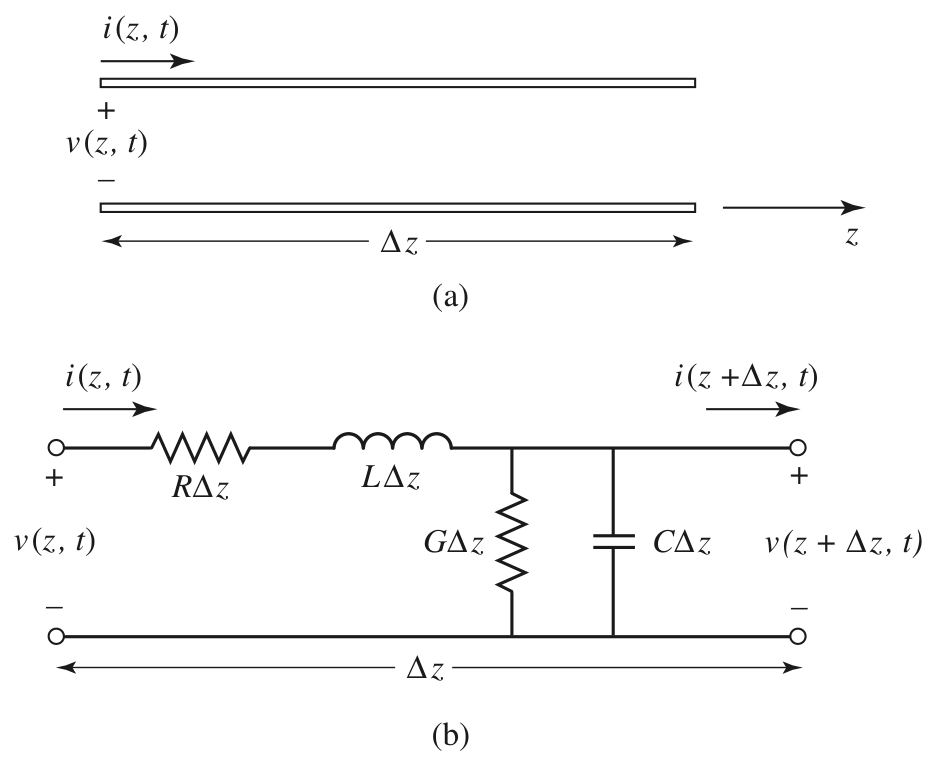
\includegraphics[width=0.62\linewidth]{figs/c2_lumped_model.png}\hfill\mbox{}\par
{\color{sub}\scriptsize (a) $v$, $i$ on a length $\Delta z$; (b) its equivalent cell. Draw (b)
before writing KVL and KCL. Pozar Fig 2.1.}
\begin{itemize}
  \item A length $\Delta z$ of line is modelled by series $R'\Delta z$, $L'\Delta z$ and
    shunt $G'\Delta z$, $C'\Delta z$, all \textbf{per unit length}.
  \item Applying KVL and KCL to that cell and letting $\Delta z \rightarrow 0$:
    \[ \frac{\partial v}{\partial z} = -R'i - L'\frac{\partial i}{\partial t},
       \qquad
       \frac{\partial i}{\partial z} = -G'v - C'\frac{\partial v}{\partial t} \]
  \item In phasor form these decouple into the \textbf{wave equations}
    \[ \frac{d^2V}{dz^2} = \gamma^2 V, \qquad \frac{d^2I}{dz^2} = \gamma^2 I \]
  \item \textbf{Propagation constant} and \textbf{characteristic impedance}:
    \[ \gamma = \alpha + j\beta = \sqrt{(R'+j\omega L')(G'+j\omega C')} \]
    \[ Z_0 = \sqrt{\frac{R'+j\omega L'}{G'+j\omega C'}} \]
  \item Solution: $V(z) = V_0^{+}e^{-\gamma z} + V_0^{-}e^{+\gamma z}$ --- a forward and a
    reflected travelling wave.
\end{itemize}
\lead{Lossless line ($R'=G'=0$) --- used for every PYQ in this chapter}
\begin{itemize}
  \item $\alpha = 0$, \quad $\beta = \omega\sqrt{L'C'}$, \quad
        $Z_0 = \sqrt{L'/C'}$ (\textbf{purely real}).
  \item $\lambda = 2\pi/\beta = v_p/f$, \quad $v_p = 1/\sqrt{L'C'} = c/\sqrt{\epsilon_r}$.
\end{itemize}
\lead{Distortionless line}
\begin{itemize}
  \item Condition: $R'C' = L'G'$. Then $\alpha = \sqrt{R'G'}$ is frequency-independent and
    $\beta = \omega\sqrt{L'C'}$ is linear in $\omega$, so all frequencies travel at the same
    $v_p$ and the pulse shape survives.
\end{itemize}}{%
\lead{Terminated line: the four quantities every problem needs}
\begin{itemize}
  \item \textbf{Load reflection coefficient}
    \[ \Gamma_L = \frac{Z_L - Z_0}{Z_L + Z_0} = \frac{z_L - 1}{z_L + 1},
       \qquad z_L = \frac{Z_L}{Z_0} \]
  \item \textbf{At a distance $d$ toward the generator}, only the phase changes on a
    lossless line:
    \[ \Gamma(d) = \Gamma_L\,e^{-j2\beta d}, \qquad |\Gamma(d)| = |\Gamma_L| \]
    This is why the Smith chart works: moving along the line is a \emph{rotation at
    constant radius}.
  \item \textbf{VSWR}
    \[ S = \frac{V_{\max}}{V_{\min}} = \frac{1+|\Gamma_L|}{1-|\Gamma_L|},
       \qquad 1 \le S \le \infty \]
  \item \textbf{Input impedance}
    \[ Z_{in}(d) = Z_0\,\frac{Z_L + jZ_0\tan\beta d}{Z_0 + jZ_L\tan\beta d} \]
  \item \textbf{Return loss} $= -20\log_{10}|\Gamma|$ dB;
    \textbf{mismatch loss} $= -10\log_{10}(1-|\Gamma|^2)$ dB.
\end{itemize}
\lead{Special line lengths --- memorise these}
\begin{tabularx}{\linewidth}{@{}L{2.15cm}X@{}}
\toprule
\hrow \thead{Case} & \thead{Input impedance} \\
\midrule
\textbf{Matched} $Z_L=Z_0$ & $Z_{in}=Z_0$ for any length; $\Gamma=0$, $S=1$. \\
\textbf{Short} $Z_L=0$ & $Z_{in} = jZ_0\tan\beta d$ --- purely reactive, inductive for $d<\lambda/4$. \\
\textbf{Open} $Z_L=\infty$ & $Z_{in} = -jZ_0\cot\beta d$ --- purely reactive, capacitive for $d<\lambda/4$. \\
\textbf{$d=\lambda/2$} & $Z_{in} = Z_L$ --- the line repeats every half wavelength. \\
\textbf{$d=\lambda/4$} & $Z_{in} = Z_0^2/Z_L$ --- the \textbf{quarter-wave transformer}; it \emph{inverts}, so a short looks open. \\
\textbf{$d=\lambda/8$} & $Z_{in} = Z_0\,\dfrac{Z_L+jZ_0}{Z_0+jZ_L}$ \quad ($\tan\beta d = 1$). \\
\bottomrule
\end{tabularx}
\vspace{2pt}
{\footnotesize\color{sub} A shorted or open stub is therefore a \emph{pure reactance whose
value you choose by cutting it to length} --- that single fact is the whole basis of stub
matching.}}

\penalty0\vspace{2pt}

%=======================================================================
\T{2.3 The Smith Chart}

\Q{Explain the construction of the Smith chart. What does each family of curves represent, and how is it read?}{\m{4}\m{5}\m{10}}
{\color{sub}\footnotesize \tF{5} \yr{\textbf{72 Ash}, \textbf{75 Bh}, 72 Ma, \texttt{81 Ba}, \textbf{80 Ch}} \gap$\cdot$\gap counted together with the immittance chart in \S2.4}

\sbsr{0.52}{%
\lead{What the chart is}
\begin{itemize}
  \item A plot of \textbf{normalised impedance $z = r + jx$ mapped onto the complex
    $\Gamma$ plane} by the bilinear transform
    \[ \Gamma = \frac{z-1}{z+1}, \qquad z = \frac{1+\Gamma}{1-\Gamma} \]
  \item Because $|\Gamma| \le 1$ for a passive load, the entire right half of the $z$ plane
    folds into the \textbf{unit circle} --- an infinite plane on one sheet of paper.
\end{itemize}
\lead{The two families of curves}
\begin{itemize}
  \item \textbf{Constant resistance $r$}: circles centred on
    $\left(\dfrac{r}{1+r},\,0\right)$ with radius $\dfrac{1}{1+r}$.
    All pass through the open-circuit point $\Gamma = +1$.
  \item \textbf{Constant reactance $x$}: arcs centred on
    $\left(1,\,\dfrac{1}{x}\right)$ with radius $\left|\dfrac{1}{x}\right|$.
    Upper half $= +x$ (\textbf{inductive}), lower half $= -x$ (\textbf{capacitive}).
  \item The two families are \textbf{orthogonal} everywhere they cross.
\end{itemize}
\lead{Landmarks}
\begin{itemize}
  \item \textbf{Centre} $z=1$: matched, $\Gamma=0$, $S=1$.
  \item \textbf{Left} $z=0$: short circuit, $\Gamma=-1$.
  \item \textbf{Right} $z=\infty$: open circuit, $\Gamma=+1$.
  \item \textbf{Rim} $|\Gamma|=1$: pure reactance, total reflection, $S=\infty$.
  \item Horizontal axis: $x=0$, i.e. purely resistive. To the right of centre lies
    $V_{\max}$ (and $r = S$); to the left lies $V_{\min}$ (and $r = 1/S$).
\end{itemize}
\lead{Reading it --- the five rules}
\begin{enumerate}[label=\arabic*., leftmargin=1.4em]
  \item Normalise: $z_L = Z_L/Z_0$. Plot it.
  \item $|\Gamma_L|$ = distance from centre $\div$ chart radius; its angle is read on the
    \textbf{angle of reflection coefficient} scale.
  \item Draw the \textbf{constant-$|\Gamma|$ (SWR) circle} through the point. Read $S$ where
    it cuts the right-hand real axis.
  \item \textbf{Move toward the generator = clockwise}; toward the load $=$ anticlockwise.
    \textbf{One full lap is $\lambda/2$}, so a quarter turn is $\lambda/8$.
  \item Read distances on the \textbf{WTG} (wavelengths toward generator) rim scale, which
    runs $0 \rightarrow 0.5$ clockwise starting at the short-circuit point.
\end{enumerate}}{%
\figT{c2_smith_blank.png}
{\footnotesize\color{sub} The impedance chart. Constant-$r$ circles (all through the open
point) and constant-$x$ arcs; the rim carries the WTG scale, on which one complete lap is
half a wavelength of line.}}

\penalty0\vspace{2pt}

\lead{Why the chart is worth using at all}
\begin{itemize}
  \item It turns the awkward $Z_{in}$ formula into a \textbf{rotation}, and $z \rightarrow y$
    into a \textbf{half-turn} --- both done with a compass instead of complex arithmetic.
  \item $\Gamma$, $S$, $Z_{in}$, $Y_{in}$, return loss and the positions of $V_{\max}$ and
    $V_{\min}$ are all read off one diagram.
  \item It shows \emph{graphically} which matching solutions exist, and lets you pick the
    one with the shortest stub or the widest bandwidth --- something a formula does not
    show you.
\end{itemize}

\penalty0\vspace{2pt}

%=======================================================================
\T{2.4 The Immittance (Admittance) Chart}

\Q{Sketch an immittance chart. List the duality parameters and compare the two scales}{\m{2}\m{4}\m{5}\m{10}}
{\color{sub}\footnotesize \tF{5} \yr{\textbf{72 Ash}, \textbf{75 Bh}, 72 Ma, \texttt{81 Ba}, \textbf{80 Ch}} \gap$\cdot$\gap short, self-contained, and asked five times}

\sbsr{0.52}{%
\lead{The admittance chart}
\begin{itemize}
  \item Since $y = 1/z$, and
    \[ \Gamma_y = \frac{y-1}{y+1} = -\frac{z-1}{z+1} = -\Gamma_z \]
    the admittance chart is \textbf{the impedance chart rotated through
    $180^\circ$} (a $\lambda/4$ line length).
  \item So on a plain Smith chart you convert $z \rightarrow y$ by drawing a diameter
    through the point and reading the diametrically opposite intersection.
\end{itemize}
\lead{The immittance chart}
\begin{itemize}
  \item \textbf{Both grids printed on one chart}, usually in two colours: the impedance
    grid and the admittance grid superimposed.
  \item A single location then carries \textbf{two readings at once} --- $z$ on one grid,
    $y$ on the other. The $\lambda/4$ half-turn is built into the printing.
  \item \textbf{Why it matters}: stub matching is done in \emph{admittance} (shunt stubs
    add susceptance) but loads are quoted as \emph{impedance}. Without an immittance chart
    every problem costs an extra half-turn, and each half-turn is a chance to misread.
\end{itemize}
\lead{Duality parameters}
\begin{tabularx}{\linewidth}{@{}L{2.5cm}X@{}}
\toprule
\hrow \thead{Impedance grid} & \thead{Admittance grid} \\
\midrule
$z = r + jx$ & $y = g + jb$ \\
Resistance $r$ & Conductance $g$ \\
Reactance $x$ & Susceptance $b$ \\
$+x$ inductive (upper) & $+b$ \textbf{capacitive} (upper) \\
$-x$ capacitive (lower) & $-b$ \textbf{inductive} (lower) \\
Short $z=0$ at $\Gamma=-1$ & Open $y=0$ at $\Gamma=-1$ \\
Open $z=\infty$ at $\Gamma=+1$ & Short $y=\infty$ at $\Gamma=+1$ \\
Series elements add & Shunt elements add \\
$r=1$ circle & $g=1$ circle \\
\bottomrule
\end{tabularx}
\vspace{2pt}
{\footnotesize\color{sub}\textbf{Trap.} The sign convention flips: a point in the
\emph{upper} half is inductive read as an impedance but \emph{capacitive} read as an
admittance. Both are the same physical point.}}{%
\figT{c2_immittance.png}
{\footnotesize\color{sub} Immittance chart. The amber grid is the blue grid turned through
$180^\circ$; one location reads $z = 0.5+j0.7$ on the impedance grid and
$y = 0.68-j0.95$ on the admittance grid. The faint point is where $y$ would have to be read
on a plain chart --- a $\lambda/4$ turn away.}}

\penalty0\vspace{2pt}

%=======================================================================
\T{2.5 Impedance Matching: Why, and Which Technique}

\Q{Why is impedance matching necessary? Compare the different impedance matching techniques}{\m{4}\m{5}\m{6}}
{\color{sub}\footnotesize \tF{3} \yr{\textbf{78 Ch}, 74 Ma, \textbf{77 Ch}} \gap$\cdot$\gap the theory half of several double-stub questions}

\sbs{%
\lead{Why match}
\begin{itemize}
  \item \textbf{Maximum power transfer}: a matched load absorbs all incident power;
    the fraction reflected is $|\Gamma|^2$.
  \item \textbf{Protect the source}: reflected power returning to a high-power amplifier or
    a magnetron causes heating, and can destroy it.
  \item \textbf{Remove standing waves}: high VSWR means voltage peaks that cause dielectric
    breakdown and arcing, and current peaks that cause $I^2R$ loss.
  \item \textbf{Preserve receiver sensitivity}: mismatch at an LNA input degrades the noise
    figure directly.
  \item \textbf{Avoid distortion}: multiple reflections on a long line arrive delayed,
    producing ghosting and intersymbol interference.
\end{itemize}
\lead{The matching network must be lossless}
\begin{itemize}
  \item A resistive pad would ``match'' but dissipate the very power being matched.
  \item So matching uses only \textbf{reactive} elements: line lengths, stubs, lumped
    $L$ and $C$.
\end{itemize}
\figT{c2_lossless_match.png}
{\color{sub}\scriptsize The general problem: a lossless network between line $Z_0$ and load
$Z_L$, chosen so the line sees $Z_0$. Every technique in the table is one way to build the box.
Pozar Fig 5.1.}}{%
\lead{Comparison of techniques}
\begin{tabularx}{\linewidth}{@{}L{2.05cm}X X@{}}
\toprule
\hrow \thead{Technique} & \thead{How it works} & \thead{Trade-offs} \\
\midrule
\textbf{Quarter-wave transformer} & $\lambda/4$ of line with $Z_{01}=\sqrt{Z_0 Z_L}$. & Simplest, but \textbf{needs a real $Z_L$} --- a complex load must first be walked to a $V_{\max}$ or $V_{\min}$. Narrowband. \\
\textbf{L-section (lumped)} & Two reactances, series $+$ shunt. & Compact; fine below $\sim$1 GHz. Above that, component parasitics (\S1.3) dominate. \\
\textbf{Single stub} & One shunt (or series) stub at a computed distance $d$. & Matches \textbf{any} load; only line, so no lumped parts. \textbf{But $d$ must move if the load changes} --- awkward to build as an adjustable tuner. \\
\textbf{Double stub} & Two stubs at \textbf{fixed} spacing; only the lengths are tuned. & Positions are pre-set, so it makes a practical \textbf{adjustable} tuner. \textbf{But a range of loads cannot be matched} (the forbidden region). \\
\textbf{Triple stub} & Three fixed stubs. & Removes the forbidden region entirely; used in laboratory slide-screw tuners. \\
\bottomrule
\end{tabularx}
\vspace{2pt}
\lead{Advantages of double stub over single stub}
\begin{itemize}
  \item Stub \textbf{positions are fixed}; matching is done by adjusting lengths only, so
    it can be built as a mechanical tuner with two sliding shorts.
  \item No need to break into the line at a computed distance --- the connection points are
    decided at manufacture.
  \item Retunes for a new load without physically relocating anything.
  \item \textbf{Cost}: a set of load admittances (the forbidden region) is unmatchable, and
    two stubs mean a slightly narrower bandwidth.
\end{itemize}}

\penalty0\vspace{2pt}

%=======================================================================
\T{2.6 Single-Stub Tuning}

\Q{Explain the design of a single-stub shunt tuner, stating all steps with reasoning. When is a short-circuited stub preferred over an open one?}{\m{8}\m{10}\m{2+8}}
{\color{sub}\footnotesize \tF{6} \yr{\textbf{72 Ash}, \textbf{74 Bh}, 72 Ma, \textbf{76 Bh}, \textbf{79 Ch}, \textbf{\texttt{81 Bh}}} \gap$\cdot$\gap worked instances in the numerical companion}

\sbs{%
\lead{Principle}
\begin{itemize}
  \item Two degrees of freedom are needed to cancel a complex mismatch, and a single stub
    supplies exactly two: \textbf{the distance $d$ from the load to the stub}, and
    \textbf{the stub length $\ell$}.
  \item Work in \textbf{admittance}, because a shunt stub \emph{adds} its susceptance:
    \[ y_{in} = y(d) + y_{stub} = 1 + jb + (-jb) = 1 \]
  \item \textbf{Step 1 --- choose $d$} so the line admittance has unit conductance:
    $y(d) = 1 + jb$. Geometrically, walk round the SWR circle until it cuts the
    \textbf{$g=1$ circle}. It always cuts it \textbf{twice}, so there are always
    \emph{two} solutions.
  \item \textbf{Step 2 --- choose $\ell$} so the stub presents $-jb$, cancelling the
    residual susceptance and leaving $y_{in}=1$, i.e. $Z_{in}=Z_0$.
\end{itemize}
\lead{Design procedure on the chart}
\begin{enumerate}[label=\arabic*., leftmargin=1.4em]
  \item Normalise $z_L = Z_L/Z_0$ and plot it.
  \item Half-turn to $y_L$ (or read it on the admittance grid). Note its WTG reading.
  \item Draw the SWR circle through $y_L$.
  \item Move \textbf{clockwise} to each intersection with the $g=1$ circle; call them
    $y_1 = 1 - jb$ and $y_2 = 1 + jb$. The WTG difference from $y_L$ gives $d_1$ and $d_2$.
  \item The stub must supply $+jb$ and $-jb$ respectively.
  \item For the stub length, start at the \textbf{termination point of the stub} --- the
    open-circuit point ($y=0$) for an open stub, the short-circuit point ($y=\infty$) for a
    shorted stub --- and run \textbf{clockwise round the rim} to the required susceptance.
    That arc, read on the WTG scale, is $\ell$.
\end{enumerate}}{%
\lead{Analytic check (use it to verify the chart)}
\begin{itemize}
  \item With $t = \tan\beta d$ and $Z_L = R_L + jX_L$, the distance satisfies
    \[ t = \frac{X_L \pm \sqrt{R_L\big[(Z_0-R_L)^2 + X_L^2\big]/Z_0}}{R_L - Z_0} \]
    reducing to $t = -X_L/2Z_0$ when $R_L = Z_0$.
  \item Then $d/\lambda = \dfrac{1}{2\pi}\tan^{-1}t$ (add $0.5$ if negative).
  \item \textbf{Stub length from the required susceptance $b_s$}:
    \[ \frac{\ell_{open}}{\lambda} = \frac{1}{2\pi}\tan^{-1}(b_s), \qquad
       \frac{\ell_{short}}{\lambda} = \frac{-1}{2\pi}\tan^{-1}\!\left(\frac{1}{b_s}\right) \]
    always reduced modulo $0.5\lambda$.
\end{itemize}
\lead{Short-circuited or open-circuited stub?}
\begin{tabularx}{\linewidth}{@{}L{1.55cm}X@{}}
\toprule
\hrow \thead{Stub} & \thead{When it is preferred} \\
\midrule
\textbf{Short} & \textbf{Coax and waveguide.} A shorting plate is exact and radiates nothing; an open coax end radiates and has fringing capacitance, so its electrical length is not its physical length. Also easier to make adjustable (sliding short). \\
\textbf{Open} & \textbf{Microstrip and other planar lines.} Ending the strip is free; a true short needs a via drilled and plated through the substrate, which adds inductance and cost. \\
\bottomrule
\end{tabularx}
\vspace{2pt}
{\footnotesize\color{sub} The two lengths differ by exactly $\lambda/4$:
$\ell_{short} = \ell_{open} \pm \lambda/4$.}
\vspace{2pt}
\lead{Which of the two solutions to build}
\begin{itemize}
  \item Prefer the \textbf{smaller $d$}: less line between load and stub means a shorter
    high-VSWR section, hence lower loss and \textbf{wider bandwidth}.
  \item Prefer the \textbf{shorter stub} for the same reason, and for compactness.
  \item A series stub is used when the line cannot be shunted (some waveguide and
    coaxial geometries); the construction is identical but done on the \emph{impedance}
    grid against the $r=1$ circle.
\end{itemize}}

\penalty0\vspace{3pt}
\sbsr{0.56}{%
\lead{The circuit, which is what to draw}
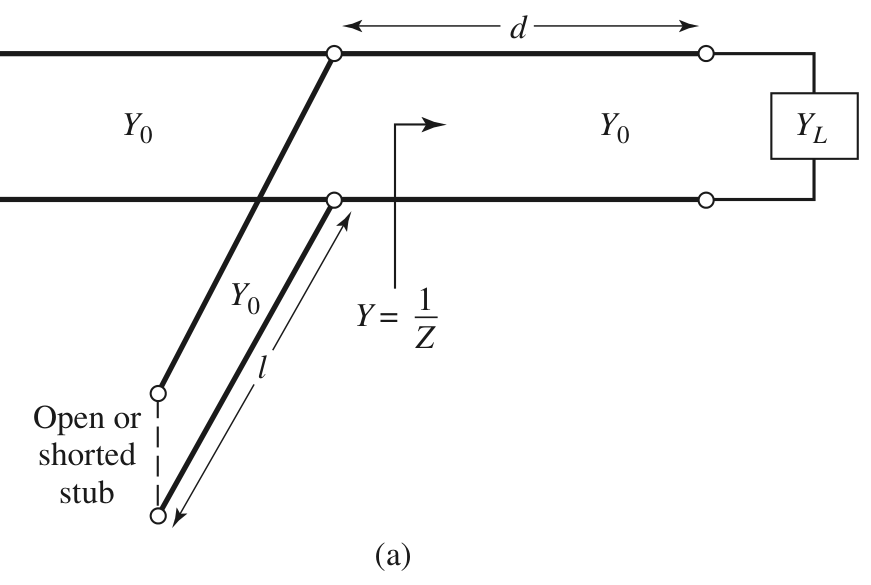
\includegraphics[width=0.49\linewidth]{figs/c2_single_stub_a.png}\hfill
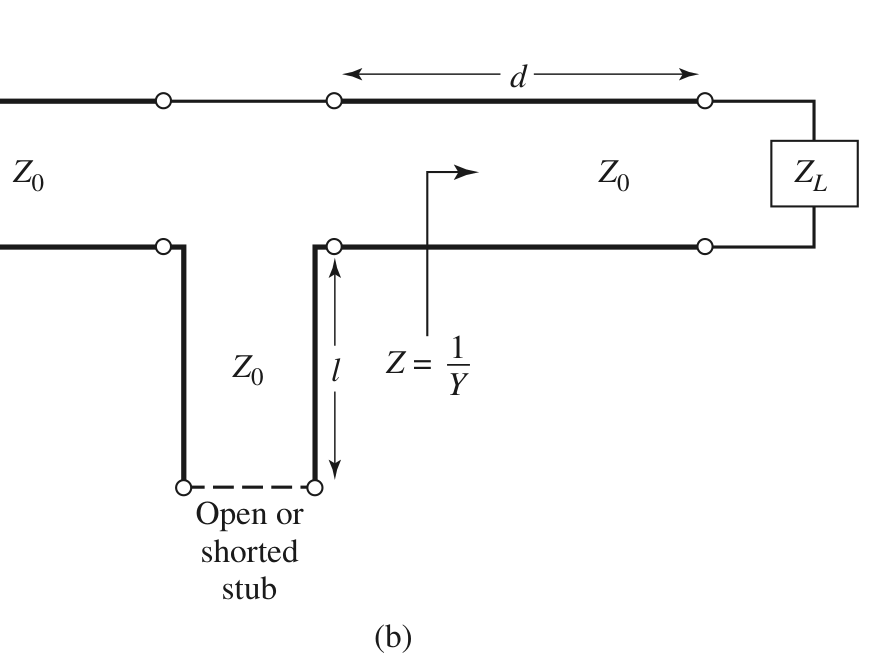
\includegraphics[width=0.49\linewidth]{figs/c2_single_stub_b.png}}{%
\vspace{2pt}
\begin{itemize}
  \item \textbf{(a) Shunt stub}: at distance $d$ from the load the line admittance is
    $Y = 1/Z = Y_0 + jB$; the stub of length $\ell$, open or shorted, adds $-jB$.
  \item \textbf{(b) Series stub}: same two unknowns $d$ and $\ell$, but the stub is in series,
    so work in impedance: $Z = Z_0 + jX$ at $d$, stub supplies $-jX$.
  \item Mark $d$ from the \textbf{load} and $\ell$ from the stub's \textbf{open or shorted
    end} on the sketch: those are the two answers the question asks for.
  \item Pozar Fig 5.4.
\end{itemize}}

\penalty0\vspace{2pt}

%=======================================================================
\T{2.7 Double-Stub Tuning}

\Q{Explain the steps for impedance matching of a load using a double-stub network. State the advantages over single-stub matching and the limitation of the technique}{\m{8}\m{10}\m{12}\m{2+8}}
{\color{sub}\footnotesize \tS{17} \yr{\textbf{69 Bh}, \textbf{70 Bh}, 70 Ma, \textbf{71 Bh}, \textbf{73 Bh}, 73 Ma, 74 Ma, \textbf{75 Bh}, \textbf{77 Ch}, \textbf{78 Ch}, \textbf{80 Ch}, \texttt{80 Ba}, \textbf{\texttt{80 Bh}}, \texttt{81 Ba}, \textbf{\texttt{79 Bh}}, \texttt{82 Ba}, \textbf{\texttt{82 Bh}}} \gap$\cdot$\gap \mk{the single most asked item in the subject}}

\sbs{%
\lead{Principle}
\begin{itemize}
  \item The two stubs sit at \textbf{fixed} positions a distance $d$ apart --- almost
    always \textbf{$\lambda/8$ or $3\lambda/8$} in the papers. Only the two lengths
    $\ell_1$ and $\ell_2$ are adjusted, and those are the two degrees of freedom.
  \item \textbf{Stub 1} cannot change the conductance it sees --- a shunt susceptance moves
    the point \emph{along its own constant-$g$ circle}. Its job is to land the point where
    the intervening $d$ of line will carry it onto the $g=1$ circle.
  \item \textbf{Stub 2} then simply cancels whatever susceptance is left, exactly as in
    single-stub matching.
\end{itemize}
\lead{The spacing circle --- the key construction}
\begin{itemize}
  \item Define the \textbf{spacing circle} as the $g=1$ circle rotated $d$
    \textbf{toward the load} (anticlockwise).
  \item Any point on it is carried \emph{onto} $g=1$ by $d$ wavelengths of line.
  \item So stub 1 must move the point from $y_1$ to the intersection of its own
    constant-$g$ circle with the spacing circle. There are generally \textbf{two}
    intersections, hence two solutions.
\end{itemize}
\lead{Design procedure}
\begin{enumerate}[label=\arabic*., leftmargin=1.4em]
  \item Normalise $z_L$, plot, half-turn to $y_L$.
  \item If the first stub is offset from the load by $d_1$, rotate $y_L$ clockwise by $d_1$
    to get $y_1$, the admittance \emph{just before} stub 1.
  \item Draw the spacing circle ($g=1$ rotated $d$ toward the load).
  \item Follow the \textbf{constant-$g$ circle through $y_1$} to its intersections with the
    spacing circle: $y_a$ and $y_a'$.
  \item $b_1 = \operatorname{Im}(y_a) - \operatorname{Im}(y_1)$ --- the susceptance stub 1
    must add. Read $\ell_1$ off the rim from the stub's termination point.
  \item Rotate $y_a$ clockwise by $d$ along its SWR circle; it lands on $g=1$ at
    $y_2 = 1 + jb_2'$.
  \item $b_2 = -b_2'$; read $\ell_2$ off the rim the same way. The network is matched.
\end{enumerate}}{%
\lead{Analytic check}
\begin{itemize}
  \item With $y_1 = g_1 + jb_L$ and $t = \tan\beta d$, requiring
    $\operatorname{Re}(y_2)=1$ after the spacing gives
    \[ \operatorname{Re}(y_2) = \frac{g_1(1+t^2)}{(1-tB)^2 + t^2g_1^2} = 1 \]
    \[ \Rightarrow \quad B = \frac{1 \pm \sqrt{g_1(1+t^2) - g_1^2t^2}}{t},
       \qquad b_1 = B - b_L \]
    where $B$ is the total susceptance after stub 1. \textbf{Note the leading $1$ in the
    numerator, not $g_1$} --- a common slip.
  \item Then $y_a = g_1 + jB$, and
    $y_2 = \dfrac{y_a + jt}{1 + jt\,y_a}$, with $b_2 = -\operatorname{Im}(y_2)$.
\end{itemize}
\lead{The forbidden region --- always state this}
\begin{itemize}
  \item The square root is real only if
    \[ g_1 \;\le\; \frac{1}{\sin^2\beta d} \]
  \item For $d = \lambda/8$ ($\beta d = 45^\circ$): $g_1 \le 2$.
    \\ \mbox{}\hfill For $d = 3\lambda/8$: $g_1 \le 2$ likewise.
    \\ \mbox{}\hfill For $d = \lambda/4$: $g_1 \le 1$.
  \item Loads whose conductance at the first stub exceeds this \textbf{cannot be matched}
    at all with that spacing. Graphically, their constant-$g$ circle lies wholly inside the
    spacing circle and never cuts it.
  \item \textbf{The fix}: add a length of line before the first stub (which moves $g_1$), or
    use a third stub.
  \item This is why $\lambda/4$ spacing is avoided in practice and $\lambda/8$ or
    $3\lambda/8$ is used --- and why the examiner keeps specifying $3\lambda/8$.
\end{itemize}
\vspace{2pt}
{\footnotesize\color{sub}\textbf{Trap.} Stub spacings near $\lambda/2$ make the two stubs
nearly coincident and the tuner hopelessly narrowband, so practical spacings stay between
$\lambda/8$ and $3\lambda/8$.}}

\penalty0\vspace{3pt}
\sbsr{0.38}{%
\lead{The circuit, which is what to draw}
\figT{c2_double_stub.png}}{%
\vspace{2pt}
\begin{itemize}
  \item \textbf{(a)} load an arbitrary distance from the first stub: stub 1 ($jB_1$, length
    $\ell_1$) nearer the load, stub 2 ($jB_2$, $\ell_2$) a fixed $d$ further toward the
    generator.
  \item \textbf{(b)} the same tuner with that offset line absorbed into the load, now called
    $Y_L'$. This is step 2 of the procedure: rotate $y_L$ by $d_1$ first, then design as if
    stub 1 sat at the load.
  \item Only $\ell_1$ and $\ell_2$ are adjusted; $d$ is fixed at manufacture, which is the
    whole advantage over one stub.
  \item Pozar Fig 5.7.
\end{itemize}}

\penalty0\vspace{2pt}

%=======================================================================
\T{2.8 S-Matrix of a Matched Network}

\Q{Prepare the scattering matrix of the network before and after matching}{\m{2}\m{2+2}\m{4}\m{6}}
{\color{sub}\footnotesize \tS{10} \yr{\textbf{76 Bh}, \textbf{77 Ch}, \textbf{78 Ch}, \texttt{80 Ba}, \textbf{\texttt{80 Bh}}, \texttt{81 Ba}, \textbf{\texttt{81 Bh}}, \textbf{\texttt{79 Bh}}, \texttt{82 Ba}, \textbf{\texttt{82 Bh}}} \gap$\cdot$\gap \mk{free marks: two lines of work, tacked onto ten stub questions}}

\sbs{%
\lead{Before matching --- a one-port}
\begin{itemize}
  \item An unmatched load seen from the line is a \textbf{one-port}, so its scattering
    matrix is the single entry
    \[ [S] = \big[\,\Gamma_L\,\big] = \left[\frac{Z_L-Z_0}{Z_L+Z_0}\right] \]
  \item Quote it in polar form, $|\Gamma_L|\angle\theta^\circ$, and give the VSWR
    alongside --- the examiner usually wants both.
\end{itemize}
\lead{After matching --- an ideal two-port}
\begin{itemize}
  \item A perfectly matched, lossless, reciprocal two-port has
    \textbf{no reflection at either port}, so $S_{11} = S_{22} = 0$, and all power passes
    through, so $|S_{12}| = |S_{21}| = 1$:
    \[ [S] = \begin{bmatrix} 0 & 1 \\ 1 & 0 \end{bmatrix} \]
  \item Keeping the electrical length $\theta = \beta\ell$ of the through path:
    \[ [S] = \begin{bmatrix} 0 & e^{-j\theta} \\ e^{-j\theta} & 0 \end{bmatrix} \]
    Either answer earns the marks; state which convention you are using.
\end{itemize}}{%
\lead{Justifying each property (this is where the marks are)}
\begin{itemize}
  \item \textbf{$S_{11}=S_{22}=0$}: that is the definition of a match --- the tuner was
    designed to make $Z_{in} = Z_0$ looking in at either port.
  \item \textbf{Reciprocity}, $S_{12} = S_{21}$: the network contains only passive,
    isotropic media (line and stubs), no ferrite and no active device, so $[S]$ is
    symmetric, $[S] = [S]^T$.
  \item \textbf{Lossless}, so $[S]$ is \textbf{unitary}:
    $[S]^{*T}[S] = [I]$, giving $\sum_k |S_{ki}|^2 = 1$ for every column. With
    $S_{11}=0$ this forces $|S_{21}| = 1$.
  \item \textbf{Reactive elements only} means no power is dissipated, only redirected --- so
    all incident power appears at the far port.
\end{itemize}
\lead{Worked shape of the answer}
\begin{itemize}
  \item ``Before: $\Gamma_L = (Z_L-Z_0)/(Z_L+Z_0) = 0.45\angle60^\circ$, so
    $[S]=[\,0.45\angle60^\circ\,]$ and $S = 2.64$.''
  \item ``After: the tuner makes $Z_{in}=Z_0$, so $S_{11}=S_{22}=0$; the network is
    reciprocal and lossless, so $S_{12}=S_{21}$ with $|S_{21}|=1$, giving
    $[S]=\left[\begin{smallmatrix}0&1\\1&0\end{smallmatrix}\right]$.''
\end{itemize}
\vspace{2pt}
{\footnotesize\color{sub} S-parameter theory in full --- properties, derivation, shifting
reference planes --- is Chapter 3. This band covers only the rider attached to stub
questions.}}

\par\penalty0\Needspace{12\baselineskip}
\sbs{%
\lead{\added{} The 3-port and 4-port version in class notes}
\begin{itemize}
  \item Some class notes draw each stub as an extra port: single stub $\rightarrow$
    $3\times3$, double stub $\rightarrow$ $4\times4$, then write ``after perfect matching''
    as a matrix whose only non-zero entry is $S_{21}$ (or $-S_{21}$ for a
    $180^\circ$ output), and ``power divided equally'' as $S_{11}/3$, $S_{21}/3$,
    $S_{31}/3$ down one column.
  \item \textbf{Do not copy those matrices.} Each fails a test of $\S$3.3:
  \begin{itemize}
    \item $S_{21} \neq 0$ with $S_{12} = 0$ is \textbf{not symmetric}, but line and stubs are
      passive and isotropic, so the network must be reciprocal.
    \item One column of $S_{k1}/3$ does not sum to $1$ in power, and the other columns are
      zero, so the matrix is \textbf{not unitary} for a lossless tuner.
  \end{itemize}
\end{itemize}}{%
\lead{\added{} What to write if the stub ports are wanted}
\begin{itemize}
  \item A stub's far end is a \textbf{short or open}, a fixed reactive termination with
    $|\Gamma| = 1$. It is not an external port, so it is absorbed into the network and the
    tuner seen from the line is the \textbf{two-port} above.
  \item Sketch the stubs as ports only to label the junctions, then reduce: before matching
    $[\,\Gamma_L\,]$, after matching
    $\left[\begin{smallmatrix}0&e^{-j\theta}\\e^{-j\theta}&0\end{smallmatrix}\right]$.
  \item Terminating the stub arm in $Z_0$ instead turns the tuner into a plain tee
    junction, and by the 3-port theorem ($\S$3.5) a tee cannot be lossless, reciprocal
    and matched at every port at once. That one line earns the extra marks.
\end{itemize}}

\penalty0\vspace{2pt}

%=======================================================================
\T{2.9 Microstrip Realisation of a Stub Tuner}

\Q{Sketch the physical diagram of the matched network using microstrips}{\m{2}\m{2+2}\m{4}}
{\color{sub}\footnotesize \tF{4} \yr{\textbf{72 Ash}, 72 Ma, \textbf{77 Ch}, \texttt{82 Ba}} \gap$\cdot$\gap turns $\lambda$ answers into millimetres}

\sbs{%
\lead{From electrical length to millimetres}
\begin{itemize}
  \item Microstrip is \textbf{quasi-TEM}, so the wave sees an effective permittivity
    between air and substrate:
    \[ \epsilon_{e} = \frac{\epsilon_r+1}{2} + \frac{\epsilon_r-1}{2}
       \frac{1}{\sqrt{1+12h/W}} \]
  \item Guide wavelength, and hence every physical length:
    \[ \lambda_g = \frac{\lambda_0}{\sqrt{\epsilon_e}} = \frac{c}{f\sqrt{\epsilon_e}},
       \qquad \ell_{\text{mm}} = \frac{\ell}{\lambda}\times\lambda_g \]
  \item \textbf{Strip width} for a wanted $Z_0$ (Hammerstad synthesis), with
    $B = \dfrac{377\pi}{2Z_0\sqrt{\epsilon_r}}$ and $W/h > 2$:
    \[ \frac{W}{h} = \frac{2}{\pi}\Big[B-1-\ln(2B-1)
       + \frac{\epsilon_r-1}{2\epsilon_r}\Big(\ln(B-1)+0.39-\frac{0.61}{\epsilon_r}\Big)\Big] \]
\end{itemize}
\lead{Layout rules the examiner looks for}
\begin{itemize}
  \item Stubs are drawn as \textbf{T-junctions off the main line}, at the computed spacing.
  \item \textbf{Open stubs} are drawn as a plain truncated strip; \textbf{shorted stubs}
    need a \textbf{via to the ground plane}, drawn as a filled circle.
  \item Label $W$ for the $Z_0$ line, the stub lengths $\ell_1$, $\ell_2$ in mm, and the
    spacing $d$ in mm.
  \item State the substrate: e.g. \textbf{RT/duroid 5880} ($\epsilon_r=2.2$),
    \textbf{FR-4} ($\epsilon_r=4.4$), \textbf{alumina} ($\epsilon_r=9.8$), with $h$.
\end{itemize}}{%
\lead{Worked conversion --- carry this shape into the exam}
\begin{itemize}
  \item Take $Z_0 = 50\,\Omega$ on FR-4, $\epsilon_r = 4.4$, $h = 1.6$ mm, $f = 3$ GHz.
  \item Synthesis gives $W/h \approx 1.9$, so $W \approx 3.0$ mm, and
    $\epsilon_e \approx 3.33$.
  \item $\lambda_0 = c/f = 100$ mm, so
    $\lambda_g = 100/\sqrt{3.33} \approx 54.8$ mm.
  \item A stub of $0.146\lambda$ is then $0.146 \times 54.8 \approx \textbf{8.0 mm}$, and a
    $3\lambda/8$ spacing is $0.375 \times 54.8 \approx \textbf{20.5 mm}$.
\end{itemize}
\lead{Practical corrections worth a mark}
\begin{itemize}
  \item \textbf{Open-end fringing}: an open stub behaves slightly longer than it is, by
    $\Delta \ell \approx 0.3\text{--}0.4\,h$. Shorten the drawn stub by that much.
  \item \textbf{T-junction discontinuity}: the junction adds shunt susceptance; the
    reference plane is not exactly the strip centreline.
  \item \textbf{Via inductance}: a shorted stub's via is not a perfect short, which is the
    practical reason open stubs dominate in microstrip.
  \item \textbf{Radiation and dispersion} rise with frequency; above about 10 GHz on FR-4
    the losses make the design impractical, so low-loss substrates are used.
\end{itemize}}

\penalty0\vspace{2pt}

%=======================================================================
\T{2.10 PYQ Mapping}

\lead{Theory questions --- covered in this document}
\begin{itemize}
  \item \textbf{Types of transmission lines; LF line vs microwave line} --- \S2.1.
    \yr{\textbf{69 Bh} \m{4}, \textbf{79 Ch} \m{10}}
  \item \textbf{Microstrip vs stripline} --- \S1.6. \yr{71 Ma \m{5}}
  \item \textbf{Smith chart construction and reading} --- \S2.3.
  \item \textbf{Immittance / admittance chart, duality, scale comparison} --- \S2.4.
    \yr{\textbf{72 Ash} \m{2}, \textbf{75 Bh} \m{10}, 72 Ma \m{5}, \texttt{81 Ba} \m{4},
    \textbf{80 Ch} \m{5}}
  \item \textbf{Impedance matching techniques compared; advantages of double over single
    stub} --- \S2.5. \yr{\textbf{78 Ch} \m{4+6}, 74 Ma \m{2+8}, \textbf{77 Ch} \m{2+8}}
  \item \textbf{Single-stub design steps and reasoning} --- \S2.6.
    \yr{\textbf{79 Ch} \m{10}, \textbf{\texttt{81 Bh}} \m{5+3+2}, \textbf{76 Bh} \m{10}}
  \item \textbf{Double-stub design steps; forbidden region} --- \S2.7.
    \yr{74 Ma \m{2+8}, \textbf{78 Ch} \m{4+6}}
  \item \textbf{S-matrix before and after matching} --- \S2.8. \yr{10 papers, see the band}
  \item \textbf{Microstrip realisation of the matched network} --- \S2.9.
    \yr{\textbf{72 Ash}, 72 Ma, \textbf{77 Ch}, \texttt{82 Ba}}
\end{itemize}

\lead{Numerical questions --- solved in the numerical companion}
\begin{itemize}
  \item \textbf{Smith chart reading} ($\Gamma_L$, VSWR, $Z_{in}$, first resistive point):
    \yr{\textbf{79 Ch}} \m{10} --- Problem 1.
  \item \textbf{Single stub} (6): \yr{\textbf{72 Ash}, \textbf{74 Bh}, 72 Ma,
    \textbf{76 Bh}, \textbf{79 Ch}, \textbf{\texttt{81 Bh}}} --- Problems 2--7.
  \item \textbf{Double stub} (17): \yr{\textbf{69 Bh}, \textbf{70 Bh}, 70 Ma, \textbf{71 Bh}, \textbf{73 Bh},
    73 Ma, 74 Ma, \textbf{75 Bh}, \textbf{77 Ch}, \textbf{78 Ch}, \textbf{80 Ch},
    \texttt{80 Ba}, \textbf{\texttt{80 Bh}}, \texttt{81 Ba}, \textbf{\texttt{79 Bh}},
    \texttt{82 Ba}, \textbf{\texttt{82 Bh}}} --- Problems 8--24.
\end{itemize}

\lead{Syllabus coverage check}
\begin{itemize}
  \item \textit{Types of transmission lines} --- \S2.1 \checkmark
  \item \textit{Transmission line theory} --- \S2.2 \checkmark
  \item \textit{Smith Chart analysis} --- \S2.3, \S2.4 \checkmark
  \item \textit{Impedance transformations and matching analysis} --- \S2.5--\S2.9
    and the numerical companion \checkmark
\end{itemize}

\penalty0\vspace{2pt}

\cleardoublepage
\section{RF and M/W Network Theory and Analysis}
{\color{sub}\footnotesize 4 hrs \gap$\cdot$\gap asked in \mk{14 of 24 papers}
\gap$\cdot$\gap 2 syllabus sub-topics \gap$\cdot$\gap \mk{128 marks, 6.2\% of the archive}
$\rightarrow$ definitions, one derivation, four matrix properties and the 3-port theorem.
The magic-tee questions are filed under Chapter 4.}

\vspace{3pt}\noindent
\colorbox{gdL}{\makebox[\dimexpr\textwidth-2\fboxsep][l]{%
  \textcolor{gd}{\bfseries\footnotesize READ THIS FIRST}}}
\par\nobreak\vspace{3pt}

Chapter 3 is the cheapest 8 to 10 marks in the paper, because the same three asks recur:
\begin{enumerate}[label=\arabic*., leftmargin=1.4em, itemsep=1pt]
  \item \textbf{Why S-parameters, and how do they differ from h / Z / Y / ABCD?}
    (12 papers) $\rightarrow$ one reason list plus one comparison table, $\S$3.1.
  \item \textbf{Derive the S-parameters of a two-port network} (7 papers)
    $\rightarrow$ the same six lines every time, $\S$3.2. Learn it as a script.
  \item \textbf{State the properties of the S-matrix and test a printed one} (6 papers)
    $\rightarrow$ \mk{four tests, always as a table}, $\S$3.3, applied to numbers in
    $\S$3.4.
\end{enumerate}
Two more traps worth knowing before the paper starts:
\begin{itemize}
  \item \textbf{Identify the passive device from its S-matrix}, the E/H-tee matrices and
    the radar power problems are filed with the tee junctions in \textbf{Chapter 4},
    $\S$4.5 to $\S$4.7. They are all the four tests of $\S$3.3 applied to a magic tee, so
    learn $\S$3.3 here first.
  \item An examiner who writes ``3-port network'' almost always wants the
    \textbf{impossibility theorem} ($\S$3.5), not just a $3\times3$ matrix. Stating that a
    3-port cannot be lossless, reciprocal and matched at the same time, and then naming the
    three escapes, is what separates a 4 from an 8.
\end{itemize}

\hr

%=======================================================================
\T{3.1 Why S-parameters: the Limits of Z, Y, h and ABCD}

\Q{Why are S-parameters used in microwave network analysis? Compare S-parameters with h-parameters}{\m{2}\m{3}\m{4}\m{4+4}\m{5+5}}
{\color{sub}\footnotesize \tS{12} \yr{\textbf{69 Bh}, \textbf{70 Bh}, 70 Ma, 73 Ma, \textbf{73 Bh}, 74 Ma, \textbf{75 Bh}, \textbf{78 Ch}, \textbf{\texttt{79 Bh}}, \texttt{80 Ba}, \textbf{\texttt{80 Bh}}, \textbf{80 Ch}} \gap$\cdot$\gap \mk{the single most repeated ask in the chapter}}

\sbs{%
\lead{What the low-frequency parameter sets need}
\begin{itemize}
  \item All four classical sets relate \textbf{total voltage and total current} at the
    terminals:
  \begin{itemize}
    \item $[V] = [Z][I]$, $Z_{ij} = V_i/I_j$ with all other ports \textbf{open}, $I_k = 0$.
    \item $[I] = [Y][V]$, $Y_{ij} = I_i/V_j$ with all other ports \textbf{shorted}, $V_k = 0$.
    \item h-parameters: mixed, $h_{11}$ and $h_{21}$ need a \textbf{short} on port 2,
      $h_{12}$ and $h_{22}$ need an \textbf{open} on port 1.
    \item ABCD: cascade form, still defined on $V$ and $I$.
  \end{itemize}
  \item Two things are therefore assumed:
  \begin{itemize}
    \item $V$ and $I$ are \textbf{unique} at a terminal pair (true only when
      $d \ll \lambda$).
    \item Ideal \textbf{open} and \textbf{short} terminations are available.
  \end{itemize}
  \item Both assumptions fail above roughly $1\,$GHz.
\end{itemize}}{%
\lead{What S-parameters do instead}
\begin{itemize}
  \item Defined on \textbf{travelling waves}, not on totals:
  \begin{itemize}
    \item $a_i$ = wave incident on port $i$, $b_i$ = wave leaving port $i$.
    \item Normalised so $|a_i|^2$ and $|b_i|^2$ \textbf{are powers}, in watts.
  \end{itemize}
  \item Every port is terminated in $Z_0$, a \textbf{matched load}:
  \begin{itemize}
    \item Easy to build and broadband, unlike open or short.
    \item No reflection back into the device $\rightarrow$ no oscillation, no damage,
      bias undisturbed.
  \end{itemize}
  \item Measured with \textbf{directional couplers} plus a vector network analyser, which
    separate incident from reflected wave and read magnitude and phase directly.
  \item Every practical figure of merit falls straight out: gain, return loss, insertion
    loss, isolation, VSWR, stability ($\S$3.4).
  \item Valid at \textbf{any} frequency, so the same formalism covers DC to mmWave.
  \item Cascadable after conversion to the transfer (T) form, so a chain of measured
    blocks can be multiplied out.
\end{itemize}}

\sbs{%
\lead{The five reasons they break at microwave}
\begin{enumerate}[label=\arabic*., leftmargin=1.4em]
  \item \textbf{No unique $V$ and $I$}:
  \begin{itemize}
    \item Circuit size is comparable to $\lambda$, so voltage varies along the conductor.
    \item In a waveguide there is no unique pair of conductors at all, so ``the voltage''
      has no single definition.
  \end{itemize}
  \item \textbf{Open and short cannot be realised}:
  \begin{itemize}
    \item A physical short has series lead inductance, an open has fringing capacitance.
    \item A short is a short at \textbf{one frequency and one reference plane} only:
      $\lambda/4$ away it looks like an open.
  \end{itemize}
  \item \textbf{Total reflection is destructive}:
  \begin{itemize}
    \item $|\Gamma| = 1$ sends all the power back into the device.
    \item Transistors and negative-resistance diodes \textbf{oscillate or burn out} under
      open or short test conditions.
  \end{itemize}
  \item \textbf{No instrument measures RF $V$ and $I$}:
  \begin{itemize}
    \item Probes load the circuit and cannot follow GHz waveforms.
    \item \textbf{Power} is what a microwave detector actually reads.
  \end{itemize}
  \item \textbf{Bias shifts}:
  \begin{itemize}
    \item Open and short terminations change the DC operating point and the junction
      capacitance of active devices, so the measurement is not of the device in use.
  \end{itemize}
\end{enumerate}}{%
\lead{h-parameters vs S-parameters}
\begin{tabularx}{\linewidth}{@{}L{2.1cm}XX@{}}
\toprule
\hrow \thead{Aspect} & \thead{h-parameters} & \thead{S-parameters} \\
\midrule
\textbf{Variables}   & Total $V$, $I$ & Incident, reflected waves $a$, $b$ \\
\textbf{Termination} & Short and open & Matched $Z_0$ \\
\textbf{Measured}    & Voltage, current & Power (magnitude + phase) \\
\textbf{Instrument}  & Curve tracer, bridge & Vector network analyser \\
\textbf{On active devices} & Oscillation, damage & Safe, bias preserved \\
\textbf{Frequency}   & Below $\approx100$ MHz & Any, chosen for RF / M/W \\
\textbf{Broadband}   & No, termination drifts & Yes \\
\textbf{Cascading}   & Awkward & Via T-matrix \\
\bottomrule
\end{tabularx}
\vspace{3pt}
\mbox{}\hfill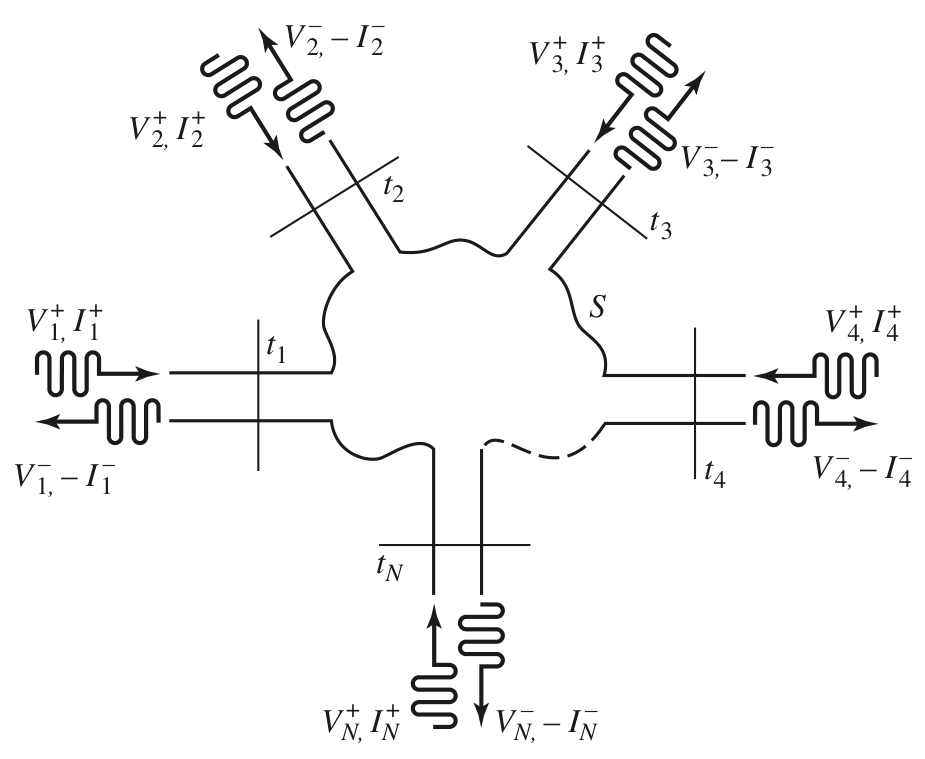
\includegraphics[width=0.46\linewidth]{figs/c3_nport.png}\hfill\mbox{}\par
{\color{sub}\scriptsize An $N$-port as S-parameters see it: at each reference plane $t_n$ an
\mk{incident} $V_n^+$ and a \mk{reflected} $V_n^-$, not one total $V$ and $I$.
Pozar Fig 4.5.}}

\penalty0\vspace{2pt}

\creamq{Answer skeleton for the 4-mark version}{\m{4}}
\begin{itemize}
  \item One line on what fails: no unique $V$ / $I$, open and short unrealisable, active
    devices damaged, no RF voltmeter.
  \item One line on the fix: normalised travelling waves measured against matched $Z_0$
    loads with directional couplers.
  \item One line on the payoff: gain, RL, IL, VSWR and stability read straight off $[S]$.
  \item Close with $[b] = [S][a]$ and the two-port matrix. Four sentences, full marks.
\end{itemize}

\penalty0\vspace{2pt}

%=======================================================================
\T{3.2 Definition and Derivation for a Two-Port Network}

\Q{Using a two-port network, define and derive the S-parameters}{\m{4}\m{5}\m{6}\m{10}}
{\color{sub}\footnotesize \tS{7} \yr{\textbf{69 Bh}, \textbf{70 Bh}, 70 Ma, \textbf{78 Ch}, \texttt{80 Ba}, \textbf{\texttt{80 Bh}}, \textbf{80 Ch}} \gap$\cdot$\gap \mk{write it as a script: figure, normalisation, matrix, four conditions}}

\sbs{%
\lead{Step 1: the wave variables}
\begin{itemize}
  \item At port $i$ the line carries a forward wave $V_i^{+}$ and a backward wave
    $V_i^{-}$. Normalise both by $\sqrt{Z_0}$:
    \[ a_i = \frac{V_i^{+}}{\sqrt{Z_0}}, \qquad b_i = \frac{V_i^{-}}{\sqrt{Z_0}} \]
  \item The normalisation is chosen so that the squared magnitudes are powers:
    \[ P_i^{\text{inc}} = \tfrac{1}{2}|a_i|^2, \qquad
       P_i^{\text{ref}} = \tfrac{1}{2}|b_i|^2 \]
    (the $\tfrac{1}{2}$ disappears if $a$, $b$ are taken as rms).
  \item In terms of the total quantities:
    \[ V_i = \sqrt{Z_0}\,(a_i + b_i), \qquad I_i = \frac{a_i - b_i}{\sqrt{Z_0}} \]
    so nothing is lost, only re-expressed.
\end{itemize}
\figC{c3_twoport.png}{0.85\linewidth}
{\footnotesize\color{sub} Port 1 and port 2 of a general two-port, each carrying an
incident wave $a$ and an emerging wave $b$. Source: RF Pulchowk Ch3 deck.}}{%
\lead{Step 2: the defining matrix}
\begin{itemize}
  \item The network is linear, so each outgoing wave is a weighted sum of all the incoming
    ones:
    \[ b_1 = S_{11}a_1 + S_{12}a_2, \qquad b_2 = S_{21}a_1 + S_{22}a_2 \]
    \[ \begin{bmatrix} b_1 \\ b_2 \end{bmatrix} =
       \begin{bmatrix} S_{11} & S_{12} \\ S_{21} & S_{22} \end{bmatrix}
       \begin{bmatrix} a_1 \\ a_2 \end{bmatrix}
       \quad\text{i.e.}\quad [b] = [S][a] \]
  \item \textbf{Subscript order}: in $S_{ij}$ the \textbf{second} index $j$ is the port
    driven, the \textbf{first} index $i$ is the port observed. $S_{21}$ is
    ``out of 2, in at 1''.
  \item Written out, the matrix is the complete input-output description of the black box:
    knowing four numbers replaces solving for every internal voltage and current.
\end{itemize}}

\sbs{%
\lead{Step 3: isolate each parameter}
\begin{itemize}
  \item Terminate the unused port in $Z_0$. A matched load reflects nothing, so its
    incident wave vanishes and one column of the matrix survives at a time.
\end{itemize}
\begin{tabularx}{\linewidth}{@{}L{2.4cm}L{1.5cm}X@{}}
\toprule
\hrow \thead{Parameter} & \thead{Condition} & \thead{Meaning} \\
\midrule
$S_{11} = \dfrac{b_1}{a_1}$ & $a_2 = 0$ & Input reflection coefficient, port 2 matched \\
$S_{21} = \dfrac{b_2}{a_1}$ & $a_2 = 0$ & Forward transmission (gain or insertion loss) \\
$S_{12} = \dfrac{b_1}{a_2}$ & $a_1 = 0$ & Reverse transmission (isolation, feedback) \\
$S_{22} = \dfrac{b_2}{a_2}$ & $a_1 = 0$ & Output reflection coefficient, port 1 matched \\
\bottomrule
\end{tabularx}
\vspace{2pt}
\begin{itemize}
  \item \mk{$a_2 = 0$ means ``port 2 terminated in $Z_0$'', never ``port 2 open''.}
    Writing ``open circuit'' here loses the mark, because it is exactly the condition
    S-parameters were invented to avoid.
\end{itemize}
\vspace{2pt}
\figC{c3_sfg.png}{0.60\linewidth}
{\footnotesize\color{sub} Signal-flow graph of the same two-port: four branches, one per
S-parameter. Useful when the question asks for a ``flow diagram''.}}{%
\lead{Step 4: tie $S_{11}$ back to impedance}
\begin{itemize}
  \item With port 2 matched, port 1 simply sees the input impedance $Z_{in}$, so
    \[ S_{11} = \Gamma_{in} = \frac{Z_{in} - Z_0}{Z_{in} + Z_0} \]
  \item This is the bridge to Chapter 2: a one-port load has the single entry
    $[S] = [\,\Gamma_L\,]$, and a perfectly matched two-port has
    $[S] = \left[\begin{smallmatrix}0&1\\1&0\end{smallmatrix}\right]$ ($\S$2.8).
\end{itemize}
\lead{Step 5: generalise to $n$ ports}
\begin{itemize}
  \item $b_i = \sum_{j=1}^{n} S_{ij}a_j$, an $n \times n$ matrix with $n^2$ entries:
    \[ S_{ij} = \left.\frac{b_i}{a_j}\right|_{a_k = 0,\ k \neq j} \]
  \item Rows and columns both equal the port count, so a 3-port gives $3\times3$ and a
    magic tee gives $4\times4$.
  \item \textbf{Reference impedance}: every entry is defined against the same $Z_0$
    (usually $50\,\Omega$), so a quoted matrix without its $Z_0$ and its frequency is
    incomplete.
\end{itemize}}

\penalty0\vspace{2pt}

%=======================================================================
\T{3.3 Properties of the S-Matrix}

\Q{State and justify the properties of the scattering matrix}{\m{4}\m{4+4}\m{5}\m{6}}
{\color{sub}\footnotesize \tF{6} \yr{\textbf{73 Bh}, \textbf{75 Bh}, \textbf{78 Ch}, \textbf{\texttt{79 Bh}}, \textbf{\texttt{80 Bh}}, \textbf{\texttt{82 Bh}}} \gap$\cdot$\gap \mk{these four tests are also the tool that identifies a device from its matrix, $\S$4.6}}

\sbs{%
\lead{P1. Zero diagonal $\Leftrightarrow$ matched port}
\begin{itemize}
  \item $S_{ii} = 0$ means a wave arriving at port $i$ is not reflected, so that port is
    matched to $Z_0$.
  \item ``Matched at all ports'' means the whole diagonal is zero.
\end{itemize}
\lead{P2. Symmetry $\Leftrightarrow$ reciprocity}
\begin{itemize}
  \item $S_{ij} = S_{ji}$ for all $i, j$, i.e. $[S] = [S]^{T}$.
  \item \textbf{Holds} for networks built of passive, linear, isotropic media: lines,
    stubs, tees, couplers, resistors, capacitors, transformers.
  \item \textbf{Fails} for magnetised ferrite (circulator, isolator, gyrator) and for
    active devices (amplifier, transistor), where $S_{21} \neq S_{12}$ by design.
  \item So a matrix that is \textbf{not} symmetric can never be a passive isotropic device.
\end{itemize}}{%
\lead{P3. Unitary $\Leftrightarrow$ lossless}
\begin{itemize}
  \item A lossless network redirects power but never dissipates it, which forces
    \[ [S]^{*T}[S] = [I] \]
  \item Reading that out column by column gives the two tests actually used in exams:
  \begin{itemize}
    \item \textbf{Column-sum test} (each column carries unit power):
      \[ \sum_{k=1}^{n} |S_{ki}|^2 = 1 \quad \text{for every } i \]
    \item \textbf{Orthogonality test} (distinct columns are orthogonal):
      \[ \sum_{k=1}^{n} S_{ki}\,S_{kj}^{*} = 0 \quad \text{for every } i \neq j \]
  \end{itemize}
  \item If a column sums to less than 1, the shortfall is the fraction of incident power
    the network \textbf{dissipates}, which is how ``is it lossless?'' is answered
    numerically ($\S$3.4 and Problem 1 of the companion).
\end{itemize}}

\sbs{%
\lead{P4. Shifting the reference plane multiplies by a phase}
\begin{itemize}
  \item Move the reference plane of port $i$ outward by an electrical length
    $\theta_i = \beta \ell_i$. Then
    \[ S'_{ij} = S_{ij}\,e^{-j(\theta_i + \theta_j)} \]
  \item Diagonal terms pick up $e^{-2j\theta_i}$, because the wave travels the added
    length twice.
  \item \textbf{Magnitudes are unchanged}: $|S'_{ij}| = |S_{ij}|$. Return loss, insertion
    loss and VSWR do not depend on where the plane is drawn; only phase does.
  \item This is why an S-parameter measurement is meaningless until the planes are
    declared, and why a VNA must be calibrated to a stated plane.
\end{itemize}
\lead{P5. Complex, frequency dependent, $n^2$ entries}
\begin{itemize}
  \item Each $S_{ij}$ carries a magnitude and an angle, and both move with frequency, so
    a quoted set is meaningless without its $f$ and its $Z_0$.
  \item An $n$-port has $n^2$ coefficients; symmetry and structural zeros cut the number
    of independent ones sharply (the magic tee has 16 entries but only 2 distinct values).
\end{itemize}
\lead{P6. Symmetric and antimetric two-ports}
\begin{itemize}
  \item \textbf{Symmetric}: reciprocal \emph{and} $S_{11} = S_{22}$. The network looks the
    same from either end.
  \item \textbf{Antimetric}: $S_{11} = -S_{22}$.
\end{itemize}}{%
\lead{The four tests as an exam checklist}
\begin{tabularx}{\linewidth}{@{}L{2.5cm}L{2.9cm}X@{}}
\toprule
\hrow \thead{Test} & \thead{Look for} & \thead{Conclusion} \\
\midrule
Diagonal & $S_{ii} = 0$? & That port is matched \\
Transpose & $[S] = [S]^{T}$? & Reciprocal (passive) or not (ferrite / active) \\
Column sums & $\sum_k|S_{ki}|^2 = 1$? & Lossless, else lossy by the shortfall \\
Column dots & $\sum_k S_{ki}S_{kj}^{*} = 0$? & Confirms lossless, ties the phases \\
\bottomrule
\end{tabularx}
\vspace{2pt}
{\footnotesize\color{sub} Run the four in this order on any matrix the examiner prints:
they are enough to name the device ($\S$4.6) and to answer every ``judge the condition''
rider.}}

\penalty0\vspace{2pt}

%=======================================================================
\T{3.4 Return Loss, Insertion Loss and the Other Figures of Merit}

\Q{Define return loss and insertion loss, and the losses associated with a two-port network}{\m{2}\m{1}\m{4}}
{\color{sub}\footnotesize \tF{3} \yr{\textbf{72 Ash}, \textbf{\texttt{79 Bh}}, \textbf{\texttt{82 Bh}}} \gap$\cdot$\gap small marks, but they are the language every other answer is written in}

\sbs{%
\lead{The three powers at a port}
\begin{itemize}
  \item $P_i$ incident, $P_r$ reflected, $P_t$ transmitted; whatever is left over is
    dissipated.
  \item Everything below is a ratio of two of those, expressed in dB and rewritten in
    terms of $[S]$.
\end{itemize}
\begin{tabularx}{\linewidth}{@{}L{2.45cm}L{3.1cm}X@{}}
\toprule
\hrow \thead{Quantity} & \thead{In terms of $[S]$} & \thead{What it tells you} \\
\midrule
\textbf{Return loss} & $RL = -20\log_{10}|S_{11}|$ &
  How well port 1 is matched. Bigger is better \\
\textbf{Insertion loss} & $IL = -20\log_{10}|S_{21}|$ &
  Power lost passing through. $0$ dB is ideal \\
\textbf{Isolation} & $-20\log_{10}|S_{12}|$ &
  Leakage backwards. Bigger is better \\
\textbf{Forward gain} & $G = 20\log_{10}|S_{21}|$ &
  Same number as $IL$, opposite sign, used for amplifiers \\
\textbf{VSWR} & $\dfrac{1+|S_{11}|}{1-|S_{11}|}$ &
  The same match on a $1$ to $\infty$ scale \\
\textbf{Reflection (mismatch) loss} & $-10\log_{10}\!\left(1-|S_{11}|^2\right)$ &
  The part of $P_i$ that never enters the network \\
\textbf{Dissipated fraction} & $1 - \sum_k |S_{k1}|^2$ &
  What the network eats. Zero for a lossless network \\
\bottomrule
\end{tabularx}
\vspace{2pt}
\begin{itemize}
  \item \textbf{Useful anchors}: $|S_{11}| = 0.5 \rightarrow RL = 6$ dB, VSWR $=3$;
    $|S_{11}| = 0.1 \rightarrow RL = 20$ dB, VSWR $= 1.22$; $|S_{11}| = 0 \rightarrow$
    perfect match, $RL = \infty$.
\end{itemize}}{%
\figT{c3_sparam_view.png}
{\footnotesize\color{sub} What each S-parameter of a device under test is called in the
lab. Source: RF Pulchowk Ch3 deck.}
\lead{Sign conventions that cost marks}
\begin{itemize}
  \item Return loss and insertion loss are quoted as \textbf{positive} dB for a passive
    device. The minus sign is already in the definition.
  \item $20\log$ for a \textbf{ratio of waves} ($S$ is an amplitude ratio),
    $10\log$ for a \textbf{ratio of powers}. Mixing the two is the commonest slip.
\end{itemize}}

\sbs{%
\lead{Reading a device off its numbers}
\begin{itemize}
  \item Small $|S_{11}|$, $|S_{22}|$ $\rightarrow$ well matched at both ends.
  \item $|S_{21}| > 1$ $\rightarrow$ \textbf{active}: the device has gain.
  \item $|S_{21}| < 1$ with $S_{12} = S_{21}$ $\rightarrow$ \textbf{passive and
    reciprocal}: an attenuator, filter or line.
  \item $|S_{12}| \ll |S_{21}|$ $\rightarrow$ \textbf{unilateral}: an amplifier or
    isolator; the smaller $|S_{12}|$ is, the more stable the amplifier tends to be.
  \item This is the whole method for \textbf{\texttt{82 Bh}}, which prints two amplifier
    S-parameter sets and asks only for ``the basic differences''. Problem 2 of the
    companion works it.
\end{itemize}}{%
\lead{\added{} Correction to the source notes}
\begin{itemize}
  \item The RF Pulchowk deck prints
    $IL\,\text{(dB)} = 10\log\left(|a_1|^2/|b_1|^2\right)$.
  \item $|b_1|$ is the wave coming \textbf{back out of port 1}, so that expression is the
    return loss, not the insertion loss.
  \item Insertion loss compares the incident wave with what leaves the \textbf{far} port:
    \[ IL = 10\log\frac{|a_1|^2}{|b_2|^2} = 20\log\frac{1}{|S_{21}|} \]
    which is what the deck's own next line prints. Use the $|S_{21}|$ form.
\end{itemize}}

\penalty0\vspace{2pt}

%=======================================================================
\T{3.5 Three-Port Networks and Why the Ideal One Cannot Exist}

\Q{Analyse a three-port network using S-parameters. Write the properties of a 3-port network and define its characteristic parameters}{\m{4}\m{4+4}\m{2+6}\m{5+2}}
{\color{sub}\footnotesize \tF{6} \yr{\textbf{72 Ash}, 73 Ma, \textbf{73 Bh}, 74 Ma, \textbf{\texttt{80 Bh}}, \textbf{\texttt{82 Bh}}} \gap$\cdot$\gap \mk{the theorem is the answer, the matrix alone is half marks}}

\sbs{%
\lead{The general 3-port}
\begin{itemize}
  \item Nine coefficients:
    \[ [S] = \begin{bmatrix} S_{11} & S_{12} & S_{13} \\
                             S_{21} & S_{22} & S_{23} \\
                             S_{31} & S_{32} & S_{33} \end{bmatrix} \]
  \item \textbf{Characteristic parameters} an examiner expects you to define:
  \begin{itemize}
    \item \textbf{Matching}: $S_{ii}$, hence return loss and VSWR at each port.
    \item \textbf{Coupling / division ratio}: $|S_{ij}|^2$, the fraction of the input
      power delivered to port $i$.
    \item \textbf{Isolation}: $-20\log|S_{ij}|$ for the pair meant to be decoupled.
    \item \textbf{Phase relation}: $\arg S_{13}$ against $\arg S_{23}$, i.e. whether the
      two output arms are in phase or in antiphase.
    \item \textbf{Insertion loss} and \textbf{bandwidth} over which all of the above hold.
  \end{itemize}
\end{itemize}
\lead{The non-reciprocal escape, drawn}
\figT{c3_circulators.png}
{\color{sub}\scriptsize (a) clockwise, (b) counterclockwise circulator with its $[S]$: zero
diagonal (matched), one unit entry per column (lossless), and $[S] \neq [S]^T$. Pozar Fig 7.2.}}{%
\lead{The three escapes, and the device each one gives}
\begin{tabularx}{\linewidth}{@{}L{2.35cm}L{2.5cm}X@{}}
\toprule
\hrow \thead{Give up} & \thead{Device} & \thead{Consequence} \\
\midrule
\textbf{Lossless} & Resistive divider, matched 3-port & All ports matched and reciprocal, but power is burnt in the resistors \\
\textbf{Reciprocal} & \textbf{Circulator} (ferrite) & Matched and lossless, but $S_{ij} \neq S_{ji}$; power circulates $1\!\to\!2\!\to\!3\!\to\!1$ \\
\textbf{Matched at every port} & \textbf{E-plane tee, H-plane tee}, T-junction & Lossless and reciprocal, but only the side arm can be matched \\
\bottomrule
\end{tabularx}
\vspace{2pt}
\begin{itemize}
  \item \textbf{Ideal circulator}, matched and lossless but not reciprocal:
    \[ [S] = \begin{bmatrix} 0&0&1 \\ 1&0&0 \\ 0&1&0 \end{bmatrix} \]
    Terminate port 3 in a matched load and it becomes an \textbf{isolator}.
  \item A \textbf{4-port} escapes the trap entirely: a directional coupler and a magic
    tee are matched, lossless \emph{and} reciprocal all at once, which is exactly why the
    exam favourite is a 4-port ($\S$4.5).
\end{itemize}}

\sbs{%
\lead{Theorem: no 3-port is lossless, reciprocal and matched at once}
\begin{itemize}
  \item \textbf{Assume all three.} Matched gives $S_{11}=S_{22}=S_{33}=0$, reciprocal
    gives $S_{ij}=S_{ji}$, so
    \[ [S] = \begin{bmatrix} 0 & S_{12} & S_{13} \\
                             S_{12} & 0 & S_{23} \\
                             S_{13} & S_{23} & 0 \end{bmatrix} \]
  \item \textbf{Apply the orthogonality test} to each pair of columns:
    \[ S_{13}^{*}S_{23} = 0, \qquad S_{12}^{*}S_{23} = 0, \qquad
       S_{12}^{*}S_{13} = 0 \]
    so at least \textbf{two} of $S_{12}, S_{13}, S_{23}$ must be zero.
  \item \textbf{Apply the column-sum test}:
    \[ |S_{12}|^2 + |S_{13}|^2 = 1, \quad |S_{12}|^2 + |S_{23}|^2 = 1, \quad
       |S_{13}|^2 + |S_{23}|^2 = 1 \]
    which requires all three to be non-zero.
  \item The two demands \textbf{contradict}, so no such network exists.
    \mk{Give up exactly one of the three properties.}
\end{itemize}}{%
\lead{E-plane tee: the worked 3-port ($\S$4.5 has the full matrix)}
\begin{itemize}
  \item Ports 1 and 2 collinear, port 3 the E-arm, assumed matched to the junction.
  \item Three physical facts start the derivation:
  \begin{itemize}
    \item An input at the E-arm splits into two outputs that are $180^\circ$
      \textbf{out of phase}: $S_{23} = -S_{13}$.
    \item Port 3 is matched: $S_{33} = 0$.
    \item The junction is passive and isotropic: $S_{ij} = S_{ji}$.
  \end{itemize}
  \item Four unknowns are left, and the unitary property fixes all four
    ($\S$4.5, and Ch4 companion Problem 6 works every line).
  \item \mk{Ports 1 and 2 cannot be matched}, and indeed the answer gives
    $S_{11} = S_{22} = 1/2$, which is the theorem showing up in the arithmetic.
\end{itemize}}

\penalty0\vspace{2pt}

%=======================================================================
\T{3.6 S-Matrices of the Two-Port and Non-Reciprocal Devices}

\Q{Evaluate the S-matrix of an amplitude modulator; know the circulator, isolator, coupler and amplifier matrices}{\m{7}}
{\color{sub}\footnotesize \tP{1} \yr{\textbf{78 Ch}} \gap$\cdot$\gap the tee and duplexer matrices are Chapter 4 material, $\S$4.5}

\sbs{%
\lead{Circulator, isolator, gyrator}
\begin{itemize}
  \item Circulator: $[S]$ as in $\S$3.5, matched and lossless but \textbf{not} symmetric.
  \item Isolator: a circulator with port 3 loaded,
    $[S] = \left[\begin{smallmatrix}0&0\\1&0\end{smallmatrix}\right]$; forward passes,
    reverse is absorbed.
  \item Gyrator: $[S] = \left[\begin{smallmatrix}0&-1\\1&0\end{smallmatrix}\right]$, a
    $180^\circ$ phase difference between the two directions.
\end{itemize}
\lead{Directional coupler}
\begin{itemize}
  \item Through arm $\alpha$, coupled arm $j\beta$, isolated arm 0, with
    $\alpha^2 + \beta^2 = 1$:
    \[ [S] = \begin{bmatrix}
       0 & \alpha & j\beta & 0 \\ \alpha & 0 & 0 & j\beta \\
       j\beta & 0 & 0 & \alpha \\ 0 & j\beta & \alpha & 0 \end{bmatrix} \]
  \item A $3$ dB coupler has $\alpha = \beta = 1/\sqrt{2}$, and is then a magic tee in
    quadrature form.
\end{itemize}}{%
\lead{Amplifier, attenuator, amplitude modulator}
\begin{itemize}
  \item Matched amplifier: $[S] = \left[\begin{smallmatrix}0&S_{12}\\S_{21}&0\end{smallmatrix}\right]$
    with $|S_{21}| > 1 \gg |S_{12}|$. Not reciprocal, not lossless.
  \item Matched attenuator of $L$ dB:
    $[S] = \left[\begin{smallmatrix}0&\alpha\\ \alpha&0\end{smallmatrix}\right]$,
    $\alpha = 10^{-L/20}$. Reciprocal but lossy.
  \item \textbf{Amplitude modulator} (\textbf{78 Ch}): the attenuator with $\alpha$
    \textbf{driven by the modulating signal}; the 7-mark answer is below.
\end{itemize}}

\par\penalty0\Needspace{16\baselineskip}
\creamq{Amplitude modulator: the 7-mark evaluation}{\m{7}}
{\color{sub}\footnotesize \yr{\textbf{78 Ch}} \gap$\cdot$\gap \added{} no source note carries it; companion Problem 3 has the same working}
\sbs{%
\lead{Model and matrix}
\begin{itemize}
  \item A two-port in the RF path: carrier in at port 1, modulated carrier out at port 2.
    The modulating signal is a \textbf{control} (bias) input, not a third RF port.
  \item Realisation: a \textbf{PIN-diode variable attenuator}. Bias sets the diode's RF
    resistance, so the modulating waveform steers the transmission.
  \item \textbf{Matched}, $S_{11} = S_{22} = 0$: built as a matched pad at every bias
    point; otherwise it pulls the source and adds incidental phase modulation.
  \item \textbf{Reciprocal}, $S_{12} = S_{21}$: a diode resistance is bilateral; no
    ferrite, no gain.
  \item \textbf{Transmission follows the message}:
    \[ \boxed{\;[S] = \begin{bmatrix} 0 & \alpha(t) \\ \alpha(t) & 0 \end{bmatrix},
       \quad \alpha(t) = \alpha_0\left(1 + m\cos\omega_m t\right)\;} \]
    $\alpha_0$ carrier-level transmission, $m$ modulation index, $\omega_m$ modulating
    frequency.
\end{itemize}}{%
\lead{Evaluate: $\alpha_0 = 0.5$, $m = 0.6$, 1 W in}
\begin{tabularx}{\linewidth}{@{}L{1.7cm}L{1.9cm}X@{}}
\toprule
\hrow \thead{Instant} & \thead{$\alpha = S_{21}$} & \thead{$IL$, $P_{out}$} \\
\midrule
Peak & $0.5(1.6) = 0.80$ & 1.94 dB, 0.64 W \\
Carrier & $0.50$ & 6.02 dB, 0.25 W \\
Trough & $0.5(0.4) = 0.20$ & 13.98 dB, 0.04 W \\
\bottomrule
\end{tabularx}
\vspace{2pt}
\begin{itemize}
  \item Column power $|S_{21}|^2 = \alpha^2 < 1$: \mk{lossy by design}. The fraction
    $1 - \alpha^2(t)$ is burnt in the diode; AM works by throwing power away in step with
    the message.
  \item Check from the matrix:
    $m = \dfrac{|S_{21}|_{\max} - |S_{21}|_{\min}}{|S_{21}|_{\max} + |S_{21}|_{\min}}
       = \dfrac{0.8 - 0.2}{0.8 + 0.2} = 0.6$ \checkmark
  \item $\alpha$ switched between 1 and 0: the same matrix is an on-off (ASK) modulator,
    $m = 1$.
\end{itemize}}

\penalty0\vspace{2pt}

%=======================================================================
\T{3.7 PYQ Mapping}

\lead{Theory questions, covered in this document}
\begin{itemize}
  \item \textbf{Why S-parameters; importance in microwave network analysis; vs
    h-parameters} $\rightarrow$ $\S$3.1.
    \mk{The most repeated topic in the chapter, 13 papers.}
    \yr{\textbf{69 Bh} \m{4}, \textbf{70 Bh} \m{4}, 70 Ma \m{4}, \textbf{80 Ch} \m{5}}
    \textbf{\texttt{81 Bh}} asks it too, \m{3}, as a rider the archive files under Chapter 1.
  \item \textbf{Derive S-parameters for a two-port network} $\rightarrow$ $\S$3.2.
    \yr{\textbf{69 Bh} \m{6}, \textbf{70 Bh} \m{4}, \texttt{80 Ba} \m{6}, \textbf{80 Ch} \m{5}}
  \item \textbf{Properties of the S-matrix} $\rightarrow$ $\S$3.3. The four tests are
    also the identification tool of $\S$4.6. \yr{\textbf{\texttt{80 Bh}} \m{4}}
  \item \textbf{Return loss and insertion loss} $\rightarrow$ $\S$3.4.
    \yr{\textbf{72 Ash} \m{2}, \textbf{\texttt{79 Bh}} \m{1}}
  \item \textbf{Three-port network: analysis, properties, characteristic parameters}
    $\rightarrow$ $\S$3.5, with the impossibility theorem and its three escapes.
    \yr{\textbf{72 Ash} \m{5}, 73 Ma \m{4}, \textbf{73 Bh} \m{4}, 74 Ma \m{6},
    \textbf{\texttt{82 Bh}} \m{4}}
  \item \textbf{Three-port parameters using an E-plane tee example} $\rightarrow$ $\S$3.5
    for the parameters, $\S$4.5 for the matrix, Ch4 companion Problem 6 for the derivation.
    \yr{\textbf{\texttt{80 Bh}} \m{4}}
  \item \textbf{Compare two printed S-parameter sets} $\rightarrow$ $\S$3.4 and companion
    Problem 2. \yr{\textbf{\texttt{82 Bh}} \m{4}}
  \item \textbf{Evaluate the S-matrix of an amplitude modulator} $\rightarrow$ $\S$3.6 and
    companion Problem 3. \added{} \yr{\textbf{78 Ch} \m{7}}
  \item \textbf{Not here}: the E-plane, H-plane and duplexer matrices, the shorted magic
    tee, identify the device from its S-matrix, and the radar power problems. The archive
    files them with the tee junctions (syllabus 4.4), so they are \textbf{Chapter 4},
    $\S$4.5 to $\S$4.7.
\end{itemize}

\lead{Numerical content}
\begin{itemize}
  \item \textbf{This chapter has a numerical companion}, \textit{Ch3 - RF and MW Network
    Theory and Analysis - Numerical Problems and Solutions}: the \textbf{\texttt{79 Bh}}
    reciprocal / lossless / return-loss / reflected-power question, the
    \textbf{\texttt{82 Bh}} comparison of two amplifier sets, and the \textbf{78 Ch}
    amplitude modulator. The tee derivations, the device identifications and the radar
    problems are in the Chapter 4 companion, Problems 6 to 17.
  \item \textbf{Not in this chapter}: amplifier stability ($K$, $\Delta$, $\mu$) and the
    unilateral / bilateral maximum gain calculations. Those ride on S-parameters but the
    archive files them under \textbf{RF Design Practices}, so they belong to Chapter 6.
    $\S$3.4 gives only the reading of the numbers that \textbf{\texttt{82 Bh}} asks for.
\end{itemize}

\par\penalty0\Needspace{7\baselineskip}
\lead{Syllabus coverage check}
\begin{itemize}
  \item \textit{Scattering matrix and its properties} $\rightarrow$ $\S$3.3, $\S$3.5,
    $\S$3.6 \checkmark
  \item \textit{S-parameter derivation and analysis} $\rightarrow$ $\S$3.1, $\S$3.2,
    $\S$3.4 \checkmark
\end{itemize}

\lead{Cross-references, so nothing is said twice}
\begin{itemize}
  \item \textbf{Chapter 1} $\S$1.2 justifies S-parameter analysis as part of the
    lumped-vs-distributed answer. The full case is $\S$3.1 here.
  \item \textbf{Chapter 2} $\S$2.8 carries the two-line S-matrix rider tacked onto ten
    stub-tuning questions ($[\Gamma_L]$ before matching, $\left[\begin{smallmatrix}0&1\\1&0\end{smallmatrix}\right]$
    after). The theory behind it is $\S$3.2 and $\S$3.3.
  \item \textbf{Chapter 4} carries the tees: construction and matrices $\S$4.5,
    identifying a device from its matrix $\S$4.6, the radar power problems $\S$4.7. The
    circulator, isolator and coupler matrices stay here in $\S$3.6.
\end{itemize}

\penalty0\vspace{2pt}

\cleardoublepage
\section{RF/Microwave Components and Devices}
{\color{sub}\footnotesize 8 hrs \gap$\cdot$\gap asked in \mk{all 24 papers}
\gap$\cdot$\gap 11 syllabus sub-topics \gap$\cdot$\gap \mk{411 marks, 19.8\% of the archive,
65 questions} \gap$\cdot$\gap \mk{124 numerical (30\%) + 287 theory}
$\rightarrow$ one derivation (the waveguide) worth up to 10 marks, one device (the magic tee)
asked 9 times by name and 8 more in disguise, and a ring of 4 to 6 mark short notes.}

\vspace{3pt}\noindent
\colorbox{gdL}{\makebox[\dimexpr\textwidth-2\fboxsep][l]{%
  \textcolor{gd}{\bfseries\footnotesize READ THIS FIRST}}}
\par\nobreak\vspace{3pt}

Chapter 4 has the biggest question count in the paper, but three scripts answer most of it:
\begin{enumerate}[label=\arabic*., leftmargin=1.4em, itemsep=1pt]
  \item \textbf{Field equations of a rectangular waveguide, TE or TM} (14 papers, up to
    \mk{10 marks}) $\rightarrow$ $\S$4.1. \mk{One seven-step script covers both modes}: only
    the boundary condition in Step 5 changes. Learn TM first; TE is the same page with
    $\sin$ and $\cos$ swapped.
  \item \textbf{Mode questions} (9 papers, 1 to 5 marks each): dominant, degenerate, ``prove
    TM$_{01}$ cannot exist'', ``show TM$_{11}$ is the lowest TM mode'' $\rightarrow$ $\S$4.2.
    Every one is \mk{the cut-off formula plus one sentence}.
  \item \textbf{Magic tee} (9 papers) $\rightarrow$ $\S$4.5, construction, derivation and
    matrix. The same matrix answers \textbf{identify the device from its S-matrix}
    (4 papers, $\S$4.6) and the \textbf{radar power problems} (4 papers, $\S$4.7):
    \mk{one matrix, three families}. The combinations (two tees joined, arms terminated
    or shorted) are worked in the numerical companion.
\end{enumerate}
Two more things worth knowing before the paper starts:
\begin{itemize}
  \item \textbf{Circular waveguide} (4 papers, 7 to 10 marks) is the rectangular script
    again in cylindrical coordinates, with Bessel functions in place of sines. The only new
    fact to memorise is the \textbf{root table} of $\S$4.3.
  \item \textbf{Short notes} rotate among circulator (3 papers), directional coupler
    (3), cavity resonator (2), Gunn diode, MASER, probe/loop coupling and microstrip (1 each).
    Each gets a ready answer below.
\end{itemize}

\hr

%=======================================================================
\T{4.1 Rectangular Waveguide: TE and TM Field Equations}

\Q{Derive the field equations and characteristic parameters of a rectangular waveguide operating in TE / TM mode}{\m{4}\m{5}\m{7+3}\m{8}\m{8+2}\m{10}}
{\color{sub}\footnotesize \tS{14} \yr{\textbf{69 Bh}, \textbf{70 Bh}, 70 Ma, \textbf{71 Bh}, 72 Ma, 74 Ma, \textbf{74 Bh}, \textbf{76 Bh}, \textbf{77 Ch}, \textbf{79 Ch}, \textbf{80 Ch}, \textbf{\texttt{80 Bh}}, \texttt{81 Ba}, \textbf{\texttt{81 Bh}}} \gap$\cdot$\gap \mk{the most repeated ask in the chapter: TE 6 papers, TM 7, modes in general 1}}

\sbsr{0.56}{%
\lead{Set-up}
\begin{itemize}
  \item Hollow metal pipe, inner broad wall $a$ along $x$, narrow wall $b$ along $y$,
    propagation along $+z$, $a > b$.
  \item Lossless dielectric $(\mu, \epsilon)$ inside, perfectly conducting walls.
  \item Symbols follow the \textbf{RF guide} (\emph{Fundamentals of Microwave Engineering},
    $\S$4.1.1, eqs 4.1 to 4.37, Liao's scheme):
  \begin{itemize}
    \item $\gamma$: intrinsic propagation constant of the dielectric; lossless
      $\Rightarrow$ $\gamma = j\omega\sqrt{\mu\epsilon}$, $\gamma^2 = -\omega^2\mu\epsilon$.
    \item $\gamma_g = \alpha_g + j\beta_g$: propagation constant \textbf{in the guide}.
    \item $k_x, k_y$: separation constants; $k_c = \sqrt{k_x^2 + k_y^2}$, cut-off wave number.
    \item $\psi$: stands for $H_z$ (TE) or $E_z$ (TM).
  \end{itemize}
  \item \textbf{No TEM mode.} With $E_z = H_z = 0$ every transverse component in Step 4 is
    zero. Physically, a closed $H$ loop in the cross-section needs an axial current, and a
    single hollow conductor has no centre conductor to carry it.
\end{itemize}}{%
\figT{c4_rect_geom.png}
{\color{sub}\scriptsize Co-ordinates of the rectangular guide. Source: Gangaju, Ch-4 deck, slide 12.}}

\lead{Step 1: wave equations (from Maxwell's equations)}
\begin{itemize}
  \item Vector wave equations:
    $\nabla^2 E = \gamma^2 E$, \quad $\nabla^2 H = \gamma^2 H$, \quad
    $\gamma = \sqrt{j\omega\mu(\sigma + j\omega\epsilon)} = \alpha + j\beta$.
  \item Each rectangular component $\psi$ obeys the scalar Helmholtz equation
    $\nabla^2\psi = \gamma^2\psi$, i.e.
    $\dfrac{\partial^2\psi}{\partial x^2} + \dfrac{\partial^2\psi}{\partial y^2}
    + \dfrac{\partial^2\psi}{\partial z^2} = \gamma^2\psi$.
\end{itemize}

\lead{Step 2: separation of variables}
\begin{itemize}
  \item Put $\psi = X(x)\,Y(y)\,Z(z)$, substitute, divide by $XYZ$:
    $\dfrac{1}{X}\dfrac{d^2X}{dx^2} + \dfrac{1}{Y}\dfrac{d^2Y}{dy^2}
    + \dfrac{1}{Z}\dfrac{d^2Z}{dz^2} = \gamma^2$.
  \item Each term is a function of one variable only $\Rightarrow$ each is a constant:
  \begin{itemize}
    \item $\dfrac{d^2X}{dx^2} = -k_x^2 X \Rightarrow X = A\sin k_x x + B\cos k_x x$.
    \item $\dfrac{d^2Y}{dy^2} = -k_y^2 Y \Rightarrow Y = C\sin k_y y + D\cos k_y y$.
    \item $\dfrac{d^2Z}{dz^2} = \gamma_g^2 Z \Rightarrow Z = e^{-\gamma_g z}$ (wave along $+z$ only).
  \end{itemize}
  \item Adding the constants back: $-k_x^2 - k_y^2 + \gamma_g^2 = \gamma^2$, so
    $\boxed{\gamma_g^2 = \gamma^2 + k_x^2 + k_y^2 = \gamma^2 + k_c^2}$.
  \item Lossless dielectric, $\gamma^2 = -\omega^2\mu\epsilon$:
    $\boxed{\gamma_g = \pm\sqrt{k_c^2 - \omega^2\mu\epsilon}}$.
\end{itemize}

\par\penalty0\Needspace{12\baselineskip}
\lead{Step 3: three cases for $\gamma_g$}
\begin{itemize}
  \item \textbf{Case I}, $\omega^2\mu\epsilon = k_c^2$: $\gamma_g = 0$, \textbf{cut-off}:
    $f_c = \dfrac{1}{2\pi\sqrt{\mu\epsilon}}\sqrt{k_x^2 + k_y^2}$.
  \item \textbf{Case II}, $\omega^2\mu\epsilon > k_c^2$:
    $\gamma_g = \pm j\beta_g = \pm j\omega\sqrt{\mu\epsilon}\sqrt{1 - (f_c/f)^2}$, imaginary
    $\rightarrow$ \textbf{propagates}; needs $f > f_c$.
  \item \textbf{Case III}, $\omega^2\mu\epsilon < k_c^2$:
    $\gamma_g = \pm\alpha_g = \pm\omega\sqrt{\mu\epsilon}\sqrt{(f_c/f)^2 - 1}$, real
    $\rightarrow$ \textbf{attenuated} as $e^{-\alpha_g z}$, carries no power; $f < f_c$.
    A waveguide is a \textbf{high-pass filter}.
  \item Final solution (propagating wave):
\end{itemize}
\[ \psi = \left[A\sin k_x x + B\cos k_x x\right]\left[C\sin k_y y + D\cos k_y y\right]e^{-j\beta_g z} \]

\par\penalty0\Needspace{14\baselineskip}
\lead{Step 4: transverse components from $E_z$ and $H_z$ (expand the curl equations)}
\begin{itemize}
  \item Every component carries $e^{-j\beta_g z}$, so $\partial/\partial z \rightarrow -j\beta_g$.
    Expand $\nabla\times E = -j\omega\mu H$ and $\nabla\times H = j\omega\epsilon E$ in
    components and solve the four transverse equations:
\end{itemize}
\[
\begin{aligned}
E_x &= -\frac{j\beta_g}{k_c^2}\frac{\partial E_z}{\partial x} - \frac{j\omega\mu}{k_c^2}\frac{\partial H_z}{\partial y}, &
E_y &= -\frac{j\beta_g}{k_c^2}\frac{\partial E_z}{\partial y} + \frac{j\omega\mu}{k_c^2}\frac{\partial H_z}{\partial x}, \\[3pt]
H_x &= -\frac{j\beta_g}{k_c^2}\frac{\partial H_z}{\partial x} + \frac{j\omega\epsilon}{k_c^2}\frac{\partial E_z}{\partial y}, &
H_y &= -\frac{j\beta_g}{k_c^2}\frac{\partial H_z}{\partial y} - \frac{j\omega\epsilon}{k_c^2}\frac{\partial E_z}{\partial x}.
\end{aligned}
\]
\begin{itemize}
  \item \mk{This block is the whole trick}: find $H_z$ (TE) or $E_z$ (TM) and the other four
    components follow by differentiation. The guide prints only the TE half (4.22) and the TM
    half (4.28 to 4.31); this is both at once.
\end{itemize}

\par\penalty0\Needspace{16\baselineskip}
\sbs{%
\lead{Step 5 (TE): $E_z = 0$, $H_z \ne 0$, so $\psi = H_z$}
\begin{itemize}
  \item With $E_z = 0$: $E_x \propto \partial H_z/\partial y$, $E_y \propto \partial H_z/\partial x$;
    tangential $E$ vanishes on the walls.
  \item $x = 0$: $E_y = 0 \Rightarrow \partial H_z/\partial x = 0 \Rightarrow A = 0$.
  \item $y = 0$: $E_x = 0 \Rightarrow \partial H_z/\partial y = 0 \Rightarrow C = 0$.
  \item $x = a$: $\sin k_x a = 0 \Rightarrow k_x = m\pi/a$.
  \item $y = b$: $\sin k_y b = 0 \Rightarrow k_y = n\pi/b$.
\end{itemize}
\[ H_z = H_{0z} \cos\frac{m\pi x}{a}\,\cos\frac{n\pi y}{b}\,e^{-j\beta_g z} \]
{\color{sub}\footnotesize $H_{0z} = BD$; $m, n \ge 0$, not both zero.}}{%
\lead{Step 5 (TM): $H_z = 0$, $E_z \ne 0$, so $\psi = E_z$}
\begin{itemize}
  \item $E_z$ is tangential to every wall, so it must vanish there.
  \item $x = 0$: $E_z = 0 \Rightarrow B = 0$.
  \item $y = 0$: $E_z = 0 \Rightarrow D = 0$.
  \item $x = a$: $\sin k_x a = 0 \Rightarrow k_x = m\pi/a$.
  \item $y = b$: $\sin k_y b = 0 \Rightarrow k_y = n\pi/b$.
\end{itemize}
\[ E_z = E_{0z} \sin\frac{m\pi x}{a}\,\sin\frac{n\pi y}{b}\,e^{-j\beta_g z} \]
{\color{sub}\footnotesize $E_{0z} = AC$; $m, n \ge 1$; $m = 0$ or $n = 0$ kills
every component.}}

\par\penalty0\Needspace{12\baselineskip}
\lead{Step 6: substitute into Step 4 (write $e^{-j\beta_g z}$ on every line in the exam)}
\textbf{TE$_{mn}$} \quad ($E_z = 0$)
\[
\begin{aligned}
H_x &= -\frac{j\beta_g}{k_c^2}\frac{\partial H_z}{\partial x} = H_{0x}\sin\frac{m\pi x}{a}\cos\frac{n\pi y}{b}\,e^{-j\beta_g z}, &
H_{0x} &= \phantom{-}\frac{j\beta_g}{k_c^2}\frac{m\pi}{a}H_{0z} \\
H_y &= -\frac{j\beta_g}{k_c^2}\frac{\partial H_z}{\partial y} = H_{0y}\cos\frac{m\pi x}{a}\sin\frac{n\pi y}{b}\,e^{-j\beta_g z}, &
H_{0y} &= \phantom{-}\frac{j\beta_g}{k_c^2}\frac{n\pi}{b}H_{0z} \\
E_x &= -\frac{j\omega\mu}{k_c^2}\frac{\partial H_z}{\partial y} = E_{0x}\cos\frac{m\pi x}{a}\sin\frac{n\pi y}{b}\,e^{-j\beta_g z}, &
E_{0x} &= \phantom{-}\frac{j\omega\mu}{k_c^2}\frac{n\pi}{b}H_{0z} \\
E_y &= \phantom{-}\frac{j\omega\mu}{k_c^2}\frac{\partial H_z}{\partial x} = E_{0y}\sin\frac{m\pi x}{a}\cos\frac{n\pi y}{b}\,e^{-j\beta_g z}, &
E_{0y} &= -\frac{j\omega\mu}{k_c^2}\frac{m\pi}{a}H_{0z}
\end{aligned}
\]

\par\penalty0\Needspace{8\baselineskip}
\textbf{TM$_{mn}$} \quad ($H_z = 0$)
\[
\begin{aligned}
E_x &= -\frac{j\beta_g}{k_c^2}\frac{\partial E_z}{\partial x} = E_{0x}\cos\frac{m\pi x}{a}\sin\frac{n\pi y}{b}\,e^{-j\beta_g z}, &
E_{0x} &= -\frac{j\beta_g}{k_c^2}\frac{m\pi}{a}E_{0z} \\
E_y &= -\frac{j\beta_g}{k_c^2}\frac{\partial E_z}{\partial y} = E_{0y}\sin\frac{m\pi x}{a}\cos\frac{n\pi y}{b}\,e^{-j\beta_g z}, &
E_{0y} &= -\frac{j\beta_g}{k_c^2}\frac{n\pi}{b}E_{0z} \\
H_x &= \phantom{-}\frac{j\omega\epsilon}{k_c^2}\frac{\partial E_z}{\partial y} = H_{0x}\sin\frac{m\pi x}{a}\cos\frac{n\pi y}{b}\,e^{-j\beta_g z}, &
H_{0x} &= \phantom{-}\frac{j\omega\epsilon}{k_c^2}\frac{n\pi}{b}E_{0z} \\
H_y &= -\frac{j\omega\epsilon}{k_c^2}\frac{\partial E_z}{\partial x} = H_{0y}\cos\frac{m\pi x}{a}\sin\frac{n\pi y}{b}\,e^{-j\beta_g z}, &
H_{0y} &= -\frac{j\omega\epsilon}{k_c^2}\frac{m\pi}{a}E_{0z}
\end{aligned}
\]
{\color{sub}\footnotesize All eight components are checked in \code{src/wg.py} against both curl
equations and against tangential $E = 0$ on all four walls; a single flipped sign fails the
check.}

\par\penalty0\Needspace{20\baselineskip}
\lead{Step 7: the characteristic equations (the ``+2'' or ``+3'' of every version)}
\begin{tabularx}{\linewidth}{@{}L{3.8cm}L{7.2cm}X@{}}
\toprule
\hrow \thead{Quantity} & \thead{Expression} & \thead{Note} \\
\midrule
Cut-off wave number & $k_c^2 = \left(\tfrac{m\pi}{a}\right)^2 + \left(\tfrac{n\pi}{b}\right)^2 = \omega_c^2\mu\epsilon$ & TE and TM alike \\
Cut-off frequency & $f_c = \dfrac{1}{2\sqrt{\mu\epsilon}}\sqrt{\left(\tfrac{m}{a}\right)^2 + \left(\tfrac{n}{b}\right)^2}$ & from $k_c = \omega_c\sqrt{\mu\epsilon}$; air: $\tfrac{c}{2}\sqrt{\cdot}$ \\
Cut-off wavelength & $\lambda_c = \dfrac{2\pi}{k_c} = \dfrac{1}{\sqrt{(m/2a)^2 + (n/2b)^2}}$ & TE$_{10}$: $\lambda_c = 2a$ \\
Phase constant & $\beta_g = \sqrt{\omega^2\mu\epsilon - k_c^2} = \omega\sqrt{\mu\epsilon}\sqrt{1 - (f_c/f)^2}$ & above cut-off \\
Guide wavelength & $\lambda_g = \dfrac{2\pi}{\beta_g} = \dfrac{\lambda}{\sqrt{1 - (f_c/f)^2}}$ & $\dfrac{1}{\lambda^2} = \dfrac{1}{\lambda_g^2} + \dfrac{1}{\lambda_c^2}$ \\
Phase velocity in guide & $v_g = \dfrac{\omega}{\beta_g} = \dfrac{v_p}{\sqrt{1 - (f_c/f)^2}}$ & $> v_p$; guide's name, see below \\
Group velocity & $v_{gr} = \dfrac{d\omega}{d\beta_g} = v_p\sqrt{1 - (f_c/f)^2}$ & $< v_p$; $v_g v_{gr} = v_p^2$ \\
Wave impedance, TE & $Z_g = \dfrac{E_x}{H_y} = -\dfrac{E_y}{H_x} = \dfrac{\omega\mu}{\beta_g} = \dfrac{\eta}{\sqrt{1 - (f_c/f)^2}}$ & $> \eta$ \\
Wave impedance, TM & $Z_g = \dfrac{E_x}{H_y} = -\dfrac{E_y}{H_x} = \dfrac{\beta_g}{\omega\epsilon} = \eta\sqrt{1 - (f_c/f)^2}$ & $< \eta$ \\
\bottomrule
\end{tabularx}
\vspace{2pt}
\begin{itemize}
  \item $v_p = 1/\sqrt{\mu\epsilon}$ is the phase velocity in the unbounded dielectric,
    $\eta = \sqrt{\mu/\epsilon}$ the intrinsic impedance; for air $v_p = c$ and
    $\eta_0 = 120\pi \approx 377\,\Omega$.
  \item \mk{Name clash}: the guide's $v_g$ is the phase velocity \textbf{in the guide}
    (Liao's name). The companion and most books use $v_p$ for that and $v_g$ for group
    velocity. Say which one you mean in the exam.
  \item Other decks: Gangaju writes $h$ for $k_c$ and $\gamma$ for $\gamma_g$; Pozar writes
    $k_c$, $\beta$, $Z_{TE}$ / $Z_{TM}$.
\end{itemize}

\par\penalty0\Needspace{14\baselineskip}
\lead{RF guide misprints (book pp.\ 32 to 36), corrected above}
{\footnotesize
\begin{itemize}
  \item (4.1) $\gamma = \sqrt{j\omega\mu(\sigma + \omega\epsilon)}$: the $j$ is missing,
    $\sigma + j\omega\epsilon$.
  \item (4.6) prints $\frac{1}{X}$ in front of all three terms: it is $\frac{1}{X}$,
    $\frac{1}{Y}$, $\frac{1}{Z}$.
  \item (4.9), (4.12) $Z'' = -k_z^2 Z$ with a $\sin$/$\cos$ solution contradict its own
    $\gamma_g$ in (4.14) and $e^{-j\beta_g z}$ in (4.19): $Z'' = \gamma_g^2 Z$, $Z = e^{-\gamma_g z}$.
  \item (4.15) $\gamma_g = \pm\sqrt{\omega_c^2\mu\epsilon - k_c^2}$: root inverted and $\omega_c$
    for $\omega$; it is $\pm\sqrt{k_c^2 - \omega^2\mu\epsilon}$. Cases II and III also print
    $\omega_c$ where $\omega$ is meant.
  \item (4.18) $\gamma_g = \pm j\alpha_g$: attenuation is real, $\gamma_g = \pm\alpha_g$.
  \item (4.19) prints $\sin$ in all four places: second term of each bracket is $\cos$.
  \item (4.22) $E_y = -\frac{j\omega\mu}{k_c^2}\frac{\partial H_z}{\partial y}$: two errors, it is
    $+\frac{j\omega\mu}{k_c^2}\frac{\partial H_z}{\partial x}$.
    TE boundary conditions are skipped entirely; Step 5 supplies them.
  \item (4.24), (4.35) $\lambda_g = 1/\sqrt{1 - (f_c/f)^2}$: numerator $\lambda$ is missing.
  \item (4.26) $Z_g = E_x/E_y$: it is $E_x/H_y$.
  \item (4.29) TM $E_y$ amplitude labelled $H_{0y}$: it is $E_{0y}$.
  \item (4.31) $H_y = +\frac{j\omega\epsilon}{k_c^2}\frac{\partial E_z}{\partial x}$: sign is $-$.
\end{itemize}}
{\color{sub}\footnotesize Gangaju deck slide 18 prints $k_y = n\pi/a$; it is $n\pi/b$.}

\par\penalty0\Needspace{12\baselineskip}
\creamq{Answer skeleton for the 4 to 5 mark short-note version}{\m{4}\m{5}}
\begin{itemize}
  \item Figure of the guide with $a$, $b$, $z$ (1 line).
  \item Helmholtz equation, $\psi = XYZ$, and $\gamma_g^2 = \gamma^2 + k_c^2$ in two lines.
  \item The one boundary-condition result ($H_z = H_{0z}\cos\cos$ for TE,
    $E_z = E_{0z}\sin\sin$ for TM).
  \item The four transverse components from Step 6, without re-deriving them.
  \item $f_c$ and $Z_g$. For the 10-mark version add Steps 2 to 5 in full and the whole
    Step 7 table.
\end{itemize}

\penalty0\vspace{2pt}

%=======================================================================
\T{4.2 Modes: Dominant, Degenerate, and the Short Proofs}

\Q{Dominant and degenerate modes; show which modes cannot exist; compare modes by cut-off}{\m{1+1+2}\m{2}\m{2+2}\m{3}\m{5}}
{\color{sub}\footnotesize \tS{9} \yr{\textbf{70 Bh}, 70 Ma, \textbf{71 Bh}, 72 Ma, \textbf{72 Ash}, \textbf{\texttt{80 Bh}}, \textbf{\texttt{81 Bh}}, \texttt{82 Ba}, \textbf{\texttt{82 Bh}}} \gap$\cdot$\gap every one is the $f_c$ formula plus one sentence}

\sbs{%
\lead{Definitions}
\begin{itemize}
  \item \textbf{Mode}: one allowed field pattern, labelled by the integers $m, n$ =
    number of half-cycle variations across $a$ and across $b$.
  \item \textbf{Dominant mode}: the mode with the \textbf{lowest cut-off frequency}.
  \begin{itemize}
    \item Rectangular guide ($a > b$): \mk{TE$_{10}$}, $f_c = c/2a$, $\lambda_c = 2a$.
    \item Circular guide: \mk{TE$_{11}$}, $f_c = 1.841\,c/2\pi r$ ($\S$4.3).
    \item Between $f_{c,10}$ and the next cut-off only the dominant mode propagates
      $\rightarrow$ \textbf{single-mode} operation, the reason guides are sized this way.
  \end{itemize}
\end{itemize}}{%
\figT{c4_te_patterns.png}
{\color{sub}\scriptsize E and H field of TE$_{10}$, TE$_{20}$, TE$_{01}$: one, two and one
half-cycles across the walls. Source: Gangaju, slide 20.}}

\sbs{%
\begin{itemize}
  \item \textbf{Degenerate modes}: \textbf{different} field patterns with the \textbf{same}
    cut-off frequency.
  \begin{itemize}
    \item TE$_{mn}$ and TM$_{mn}$ for every $m, n \ge 1$: same $f_c$ formula.
    \item Square guide ($a = b$): TE$_{10}$ and TE$_{01}$ as well.
    \item Circular guide: TE$_{01}$ and TM$_{11}$ (both root 3.832).
    \item Unwanted, because power can couple between them at any discontinuity.
  \end{itemize}
\end{itemize}}{%
\figT{c4_cutoff_line.png}
{\color{sub}\scriptsize Cut-off ladder, Gangaju slide 22 (from Sadiku). The slide's caption
says $a = 2.5$ cm, $b = 1$ cm; the arrows (TE$_{10}$ at 3 GHz, TE$_{20}$ at 6,
TE$_{50}$ and TE$_{02}$ at 15) are those of a \textbf{5 cm $\times$ 2 cm} guide.
TM arrows below the line sit on their TE twins: degeneracy. \added{}}}

\par\penalty0\Needspace{10\baselineskip}
\creamq{Prove that TM$_{01}$ and TM$_{10}$ modes do not exist}{\m{3}}
{\color{sub}\footnotesize \yr{70 Ma}}
\begin{itemize}
  \item TM: $H_z = 0$ and $E_z = E_{0z}\sin(m\pi x/a)\sin(n\pi y/b)e^{-j\beta_g z}$.
  \item $m = 0$ or $n = 0$ $\Rightarrow$ $\sin 0 = 0$ $\Rightarrow$ $E_z = 0$ everywhere.
  \item Every transverse component is a derivative of $E_z$ (Step 4 with $H_z = 0$)
    $\Rightarrow$ $E_x = E_y = H_x = H_y = 0$.
  \item All six components vanish $\Rightarrow$ \mk{no field, no mode}. TM$_{mn}$ needs
    $m \ge 1$ \textbf{and} $n \ge 1$.
\end{itemize}

\par\penalty0\Needspace{9\baselineskip}
\creamq{Prove that the lowest cut-off TM mode is TM$_{11}$}{\m{3}}
{\color{sub}\footnotesize \yr{\textbf{\texttt{82 Bh}}}}
\begin{itemize}
  \item From above, TM needs $m, n \ge 1$.
  \item $f_c = \frac{c}{2}\sqrt{(m/a)^2 + (n/b)^2}$ grows with both $m$ and $n$.
  \item Smallest admissible pair is $m = n = 1$:
    $\boxed{f_{c,TM_{11}} = \frac{c}{2}\sqrt{\frac{1}{a^2} + \frac{1}{b^2}}}$, for any $a, b$.
\end{itemize}

\par\penalty0\Needspace{15\baselineskip}
\creamq{Show that the dominant TE mode is TE$_{10}$; compare TE$_{10}$ with TE$_{20}$}{\m{2}\m{3}}
{\color{sub}\footnotesize \yr{\textbf{71 Bh}, \textbf{\texttt{81 Bh}}}}
\sbs{%
\begin{itemize}
  \item TE: $H_z = H_{0z}\cos\cos$ survives with one index zero ($\cos 0 = 1$); only
    TE$_{00}$ is excluded (constant $H_z$, all transverse components zero).
  \item Two candidates for the lowest $f_c$:
    $f_{c,10} = \dfrac{c}{2a}$, \quad $f_{c,01} = \dfrac{c}{2b}$.
  \item $a > b \Rightarrow f_{c,10} < f_{c,01}$ $\Rightarrow$ \mk{TE$_{10}$ is dominant}.
    It also beats TM$_{11}$, since $\frac{1}{a^2} < \frac{1}{a^2} + \frac{1}{b^2}$.
  \item \textbf{81 Bh prints ``when $b > a$''.} With $b > a$ it is TE$_{01}$ that is
    dominant; TE$_{10}$ needs $a > b$. The paper has the inequality reversed. Prove the
    $a > b$ case and state this. \added{}
\end{itemize}}{%
\begin{tabularx}{\linewidth}{@{}L{1.9cm}XX@{}}
\toprule
\hrow & \thead{TE$_{10}$} & \thead{TE$_{20}$} \\
\midrule
$f_c$ & $c/2a$ & $c/a = 2f_{c,10}$ \\
$\lambda_c$ & $2a$ & $a$ \\
Variation across $a$ & one half-cycle & two half-cycles \\
Field components & $E_y, H_x, H_z$ only & same three \\
Status & \mk{dominant} & higher-order \\
\bottomrule
\end{tabularx}
\vspace{2pt}
\begin{itemize}
  \item Single-mode band: $c/2a < f < c/a$ provided $a \ge 2b$ (otherwise TE$_{01}$
    arrives first at $c/2b$).
\end{itemize}}

\par\penalty0\Needspace{11\baselineskip}
\creamq{Dominant vs degenerate modes; for $a = 3b$ find the dominant mode among TM$_{01}$, TM$_{10}$, TM$_{11}$, TM$_{21}$, TM$_{12}$, TM$_{02}$, TM$_{20}$}{\m{2+2}\m{3}}
{\color{sub}\footnotesize \yr{72 Ma, \texttt{82 Ba}} \gap$\cdot$\gap full working in the companion, Problem 4}
\begin{itemize}
  \item With $a = 3b$: $f_c = \dfrac{c}{2a}\sqrt{m^2 + 9n^2}$.
  \item TM$_{01}$, TM$_{10}$, TM$_{02}$, TM$_{20}$ \textbf{do not exist} (an index is zero).
  \item TM$_{11}$: $\sqrt{10} = 3.162$; TM$_{21}$: $\sqrt{13} = 3.606$;
    TM$_{12}$: $\sqrt{37} = 6.083$ (in units of $c/2a$).
  \item \mk{Dominant among those listed: TM$_{11}$.} (Overall, TE$_{10}$ at 1 unit.)
\end{itemize}

\par\penalty0\Needspace{9\baselineskip}
\creamq{Cut-off checks: does the guide pass the signal?}{\m{1+1+2}\m{3}\m{5}}
{\color{sub}\footnotesize \yr{\textbf{70 Bh}, \textbf{72 Ash}, \textbf{\texttt{80 Bh}}} \gap$\cdot$\gap worked in the companion, Problem 3}
\begin{itemize}
  \item Rule: compute $f_c$ of the \textbf{dominant} mode; the signal propagates only if
    $f > f_c$.
  \item \textbf{70 Bh}: wall separation 5 cm, TE$_{10}$: $f_c = 3$ GHz $> 1$ GHz
    $\Rightarrow$ \mk{1 GHz cannot propagate}; it decays at $59.2$ Np/m.
  \item \textbf{\texttt{80 Bh}}: width 2.254 cm: $f_c = 6.65$ GHz $> 6$ GHz $\Rightarrow$
    \mk{6 GHz is not supported}.
\end{itemize}

\penalty0\vspace{2pt}

%=======================================================================
\T{4.3 Circular Waveguide}

\Q{Field equations of a circular waveguide in TE / TM mode; TE vs TM; dominant mode}{\m{7}\m{8+2}\m{10}}
{\color{sub}\footnotesize \tF{4} \yr{71 Ma, \textbf{75 Bh}, \textbf{\texttt{79 Bh}}, \texttt{82 Ba}} \gap$\cdot$\gap the rectangular script in cylindrical co-ordinates}

\lead{Set-up}
\begin{itemize}
  \item Hollow circular pipe of inner radius $a$, co-ordinates $(\rho, \phi, z)$,
    fields $\propto e^{-j\beta z}$; $k_c^2 = k^2 - \beta^2$, with $k = \omega\sqrt{\mu\epsilon}$.
  \item \textbf{Step 1}, the cylindrical version of the transverse equations
    (Waveguide.pdf p8, Pozar $\S$3.4):
\end{itemize}
\[
\begin{aligned}
E_\rho &= -\frac{j}{k_c^2}\left(\beta\frac{\partial E_z}{\partial\rho} + \frac{\omega\mu}{\rho}\frac{\partial H_z}{\partial\phi}\right), &
E_\phi &= -\frac{j}{k_c^2}\left(\frac{\beta}{\rho}\frac{\partial E_z}{\partial\phi} - \omega\mu\frac{\partial H_z}{\partial\rho}\right), \\
H_\rho &= \phantom{-}\frac{j}{k_c^2}\left(\frac{\omega\epsilon}{\rho}\frac{\partial E_z}{\partial\phi} - \beta\frac{\partial H_z}{\partial\rho}\right), &
H_\phi &= -\frac{j}{k_c^2}\left(\omega\epsilon\frac{\partial E_z}{\partial\rho} + \frac{\beta}{\rho}\frac{\partial H_z}{\partial\phi}\right).
\end{aligned}
\]

\sbsr{0.40}{%
\figT{c4_circ_cavity.png}
{\color{sub}\scriptsize Cylindrical co-ordinates. The figure is a circular cavity (a guide
closed at both ends, $\S$4.10); the guide itself is the same cylinder, open along $z$.
Source: Gangaju, slide 93.}}{%
\lead{Step 2 and 3: separate the Helmholtz equation}
\begin{itemize}
  \item $\dfrac{\partial^2 h_z}{\partial\rho^2} + \dfrac{1}{\rho}\dfrac{\partial h_z}{\partial\rho}
    + \dfrac{1}{\rho^2}\dfrac{\partial^2 h_z}{\partial\phi^2} + k_c^2 h_z = 0$.
  \item $h_z = R(\rho)P(\phi)$:
  \begin{itemize}
    \item $P'' + n^2 P = 0 \Rightarrow P = A\sin n\phi + B\cos n\phi$; $n$ an
      \textbf{integer} because the field repeats every $2\pi$.
    \item $\rho^2R'' + \rho R' + (k_c^2\rho^2 - n^2)R = 0$: \textbf{Bessel's equation}
      $\Rightarrow R = C J_n(k_c\rho) + D Y_n(k_c\rho)$.
    \item $Y_n \rightarrow \infty$ at $\rho = 0$ $\Rightarrow$ $D = 0$.
  \end{itemize}
\end{itemize}}

\par\penalty0\Needspace{20\baselineskip}
\sbs{%
\lead{TE$_{nm}$: $E_z = 0$}
\begin{itemize}
  \item $H_z = (A\sin n\phi + B\cos n\phi)\,J_n(k_c\rho)\,e^{-j\beta z}$.
  \item \textbf{Boundary}: $E_\phi(\rho = a) = 0$. Since $E_\phi \propto \partial H_z/\partial\rho$:
    $J_n'(k_c a) = 0 \Rightarrow \boxed{k_c = p'_{nm}/a}$, $p'_{nm}$ = $m$-th root of $J_n'$.
\end{itemize}
\[
\begin{aligned}
E_\rho &= \frac{-j\omega\mu n}{k_c^2\rho}(A\cos n\phi - B\sin n\phi)J_n(k_c\rho) \\
E_\phi &= \frac{j\omega\mu}{k_c}(A\sin n\phi + B\cos n\phi)J_n'(k_c\rho) \\
H_\rho &= \frac{-j\beta}{k_c}(A\sin n\phi + B\cos n\phi)J_n'(k_c\rho) \\
H_\phi &= \frac{-j\beta n}{k_c^2\rho}(A\cos n\phi - B\sin n\phi)J_n(k_c\rho)
\end{aligned}
\]
\begin{itemize}
  \item $f_{c} = \dfrac{p'_{nm}}{2\pi a\sqrt{\mu\epsilon}}$, \quad
    $Z_{TE} = \dfrac{E_\rho}{H_\phi} = \dfrac{\omega\mu}{\beta} = \dfrac{\eta k}{\beta}$.
\end{itemize}}{%
\lead{TM$_{nm}$: $H_z = 0$}
\begin{itemize}
  \item $E_z = (A\sin n\phi + B\cos n\phi)\,J_n(k_c\rho)\,e^{-j\beta z}$.
  \item \textbf{Boundary}: $E_z(\rho = a) = 0$ directly:
    $J_n(k_c a) = 0 \Rightarrow \boxed{k_c = p_{nm}/a}$, $p_{nm}$ = $m$-th root of $J_n$.
\end{itemize}
\[
\begin{aligned}
E_\rho &= \frac{-j\beta}{k_c}(A\sin n\phi + B\cos n\phi)J_n'(k_c\rho) \\
E_\phi &= \frac{-j\beta n}{k_c^2\rho}(A\cos n\phi - B\sin n\phi)J_n(k_c\rho) \\
H_\rho &= \frac{j\omega\epsilon n}{k_c^2\rho}(A\cos n\phi - B\sin n\phi)J_n(k_c\rho) \\
H_\phi &= \frac{-j\omega\epsilon}{k_c}(A\sin n\phi + B\cos n\phi)J_n'(k_c\rho)
\end{aligned}
\]
\begin{itemize}
  \item $f_{c} = \dfrac{p_{nm}}{2\pi a\sqrt{\mu\epsilon}}$, \quad
    $Z_{TM} = \dfrac{E_\rho}{H_\phi} = \dfrac{\beta}{\omega\epsilon} = \dfrac{\eta\beta}{k}$.
  \item \mk{Sign}: Waveguide.pdf p11 prints $E_\phi$ with a $+$; it is $-$.
    \code{wg.py} fails the curl equation with the $+$. \added{}
\end{itemize}}

\par\penalty0\Needspace{14\baselineskip}
\sbs{%
\lead{Root table and mode order (all a circular answer needs)}
\begin{tabularx}{\linewidth}{@{}L{1.3cm}L{1.9cm}L{1.9cm}X@{}}
\toprule
\hrow \thead{Mode} & \thead{Root} & \thead{$\lambda_c$} & \thead{Order} \\
\midrule
TE$_{11}$ & $p'_{11} = 1.841$ & $3.41a$ & \mk{1st, dominant} \\
TM$_{01}$ & $p_{01} = 2.405$ & $2.61a$ & 2nd, lowest TM \\
TE$_{21}$ & $p'_{21} = 3.054$ & $2.06a$ & 3rd \\
TE$_{01}$ & $p'_{01} = 3.832$ & $1.64a$ & 4th (low-loss mode) \\
TM$_{11}$ & $p_{11} = 3.832$ & $1.64a$ & degenerate with TE$_{01}$ \\
\bottomrule
\end{tabularx}
\vspace{2pt}
{\color{sub}\footnotesize $\lambda_c = 2\pi a/p$. Roots from \code{scipy} in \code{wg.py}. Worked
example: $a = 2$ cm gives TE$_{11}$ at $4.40$ GHz and TM$_{01}$ at $5.74$ GHz (Waveguide.pdf p13).}}{%
\lead{TE vs TM in a circular guide (71 Ma)}
\begin{tabularx}{\linewidth}{@{}L{1.7cm}XX@{}}
\toprule
\hrow & \thead{TE$_{nm}$} & \thead{TM$_{nm}$} \\
\midrule
Longitudinal & $E_z = 0$, $H_z \ne 0$ & $H_z = 0$, $E_z \ne 0$ \\
Boundary & $J_n'(k_c a) = 0$ & $J_n(k_c a) = 0$ \\
Roots & $p'_{nm}$ & $p_{nm}$ \\
Dominant & TE$_{11}$, 1.841 & TM$_{01}$, 2.405 \\
Impedance & $\eta k/\beta > \eta$ & $\eta\beta/k < \eta$ \\
$m = 0$ ? & TE$_{n0}$ absent & TM$_{n0}$ absent \\
Special & TE$_{01}$: loss falls with $f$ & TM$_{01}$: symmetric, rotary joints \\
\bottomrule
\end{tabularx}
\vspace{2pt}
\begin{itemize}
  \item \textbf{75 Bh}: dominant TE mode = TE$_{11}$, dominant TM mode = TM$_{01}$, and
    TE$_{11}$ is dominant overall since $1.841 < 2.405$.
\end{itemize}}

\penalty0\vspace{2pt}

%=======================================================================
\T{4.4 Coupling Energy into a Waveguide: Probes, Loops and Slots}

\Q{Probe coupling vs loop coupling}{\m{5}}
{\color{sub}\footnotesize \tP{1} \yr{\textbf{69 Bh}} \gap$\cdot$\gap also the answer to ``how is a cavity or klystron excited''}

\sbsr{0.62}{%
\begin{tabularx}{\linewidth}{@{}L{1.55cm}XX@{}}
\toprule
\hrow & \thead{Probe} & \thead{Loop} \\
\midrule
Couples to & \textbf{E} field & \textbf{H} field \\
Acts as & quarter-wave monopole antenna & small magnetic dipole \\
Best position & centre of broad wall $a$, parallel to E lines, $\lambda_g/4$ from the shorted end (E maximum) & where H is strongest, e.g. at the shorted end; loop plane normal to H lines \\
Less coupling & shorten, move off centre, shield & rotate, or move to fewer H lines \\
Bandwidth & grows with probe diameter & grows with wire size \\
Power & door-knob probe: more area, more power & grows with loop diameter \\
Removal & same probe, reverse action & same loop, induced current \\
\bottomrule
\end{tabularx}}{%
\figT{c4_probe.png}
\vspace{2pt}

\figT{c4_loop.png}
{\color{sub}\scriptsize Probe (top) launches E lines; loop (bottom) links H lines. Source:
Gangaju, slides 3 and 6.}}
\begin{itemize}
  \item \textbf{Slot / aperture}: a hole in the wall where the field is strong; gives
    \textbf{loose} coupling, used between a guide and a cavity or a second guide
    (directional coupler, $\S$4.8).
  \item Choice depends on: voltage breakdown near an antinode, ease of adjustment,
    constancy of coupling under mechanical change, not disturbing an electron beam, matching.
\end{itemize}

\penalty0\vspace{2pt}

%=======================================================================
\T{4.5 Waveguide Tee Junctions and the Magic Tee}

\Q{Explain the magic tee with a neat diagram and derive its S-matrix; E-plane vs H-plane tee}{\m{3+3}\m{4}\m{5}\m{6}\m{8}}
{\color{sub}\footnotesize \tS{9} \yr{71 Ma, \textbf{71 Bh}, \textbf{72 Ash}, 72 Ma, \textbf{79 Ch}, \textbf{\texttt{79 Bh}}, \textbf{80 Ch}, \textbf{\texttt{80 Bh}}, \textbf{\texttt{82 Bh}}} \gap$\cdot$\gap construction, derivation and use; identification is $\S$4.6, the radar problems $\S$4.7}

\sbsr{0.42}{%
\figT{c3_magictee.png}
{\color{sub}\scriptsize Magic tee: collinear ports 1, 2; E-arm 3; H-arm 4.}}{%
\lead{Construction}
\begin{itemize}
  \item A \textbf{hybrid} of the two simple tees on one junction:
  \begin{itemize}
    \item \textbf{E-plane (series) tee}: side arm on the \textbf{broad} wall, its axis
      parallel to the main guide's E field. Port 3.
    \item \textbf{H-plane (shunt) tee}: side arm on the \textbf{narrow} wall, in the plane
      of H. Port 4.
  \end{itemize}
  \item Collinear arms 1 and 2 are symmetric about both side arms.
  \item A \textbf{post and iris} inside the junction match ports 3 and 4; without them the
    junction is simply a ``hybrid tee'' and is poorly matched.
  \item It is called \textbf{magic} because a matched 4-port with this symmetry turns out
    to be matched at \textbf{all} ports and isolates the two pairs, which nothing in its
    shape makes obvious.
\end{itemize}}

\par\penalty0\Needspace{20\baselineskip}
\lead{Derivation of the S-matrix, the 4-mark version asked in 80 Bh and 72 Ma}
\begin{enumerate}[label=\arabic*., leftmargin=1.4em, itemsep=1pt]
  \item 4 ports $\Rightarrow$ a $4\times4$ matrix $[S]$; write all sixteen $S_{ij}$ out,
    $i, j$ from 1 to 4.
  \item \textbf{H-arm symmetry}: input at 4 reaches 1 and 2 equally and \textbf{in phase}
    $\Rightarrow S_{14} = S_{24}$.
  \item \textbf{E-arm antisymmetry}: input at 3 reaches 1 and 2 equally and in
    \textbf{antiphase} $\Rightarrow S_{13} = -S_{23}$.
  \item \textbf{E and H arms are orthogonal}: an E-arm wave cannot excite the H-arm mode
    $\Rightarrow S_{34} = S_{43} = 0$.
  \item \textbf{Matched side arms} (post and iris) $\Rightarrow S_{33} = S_{44} = 0$.
  \item \textbf{Reciprocity} $\Rightarrow S_{ij} = S_{ji}$.
  \item \textbf{Unitary, column 3}: $|S_{13}|^2 + |S_{23}|^2 = 1$, with
    $|S_{13}| = |S_{23}| \Rightarrow S_{13} = 1/\sqrt{2}$. Same for column 4:
    $S_{14} = 1/\sqrt{2}$.
  \item \textbf{Unitary, column 1}: $|S_{11}|^2 + |S_{12}|^2 + \tfrac{1}{2} + \tfrac{1}{2} = 1
    \Rightarrow S_{11} = S_{12} = 0$; column 2 gives $S_{22} = 0$.
  \item Result:
    $\;[S] = \dfrac{1}{\sqrt{2}}\left[\begin{smallmatrix} 0&0&1&1\\ 0&0&-1&1\\ 1&-1&0&0\\ 1&1&0&0 \end{smallmatrix}\right]$,
    matched at all four ports, lossless, reciprocal.
\end{enumerate}

\par\penalty0\Needspace{16\baselineskip}
\sbs{%
\lead{Properties (read straight off the matrix)}
\begin{itemize}
  \item Into \textbf{H-arm} (4): equal halves at 1 and 2, \textbf{in phase}; nothing at 3.
  \item Into \textbf{E-arm} (3): equal halves at 1 and 2, \textbf{antiphase}; nothing at 4.
  \item Into \textbf{collinear} port 1: halves at 3 and 4; \textbf{nothing at 2}.
  \item Equal in-phase signals at 1 and 2: \textbf{sum} emerges at 4, nothing at 3.
  \item Equal antiphase signals at 1 and 2: \textbf{difference} emerges at 3, nothing at 4.
  \item All four ports matched: no reflection anywhere.
\end{itemize}
\lead{Applications}
\begin{itemize}
  \item Power combiner, e.g. two radar transmitters into one antenna ($\S$4.7).
  \item Duplexer: transmitter and receiver on the isolated E and H arms (below).
  \item Balanced mixer: signal on one side arm, local oscillator on the other.
  \item Impedance bridge / measurement: unknown and standard on 1 and 2, null detector on 3.
  \item Monopulse radar comparator: sum and difference channels.
\end{itemize}}{%
\lead{E-plane tee vs H-plane tee}
\begin{tabularx}{\linewidth}{@{}L{1.55cm}XX@{}}
\toprule
\hrow & \thead{E-plane (series)} & \thead{H-plane (shunt)} \\
\midrule
Side arm on & broad wall, $\parallel$ E & narrow wall, $\parallel$ H \\
Side-arm input & antiphase at 1, 2 & in phase at 1, 2 \\
Relation & $S_{13} = -S_{23}$ & $S_{13} = S_{23}$ \\
Equivalent & series junction & shunt junction \\
In-phase at 1, 2 & cancel in side arm & add in side arm \\
Matrix & $-1/\sqrt{2}$ in row 3 (below) & $-1/2$ at $S_{12}$ (below) \\
\bottomrule
\end{tabularx}
\vspace{2pt}
\begin{itemize}
  \item Both are 3-ports and \textbf{cannot} be lossless, reciprocal and matched at once
    ($\S$3.5): ports 1 and 2 stay mismatched with $|S_{11}| = 1/2$.
\end{itemize}
{\color{sub}\footnotesize \yr{\textbf{69 Bh} \m{5}, \texttt{80 Ba} \m{4}}}}

\sbsr{0.30}{%
\figT{c4_ratrace.png}}{%
\lead{Hybrid ring (rat race)}
\begin{itemize}
  \item Annular line, circumference $1.5\lambda_g$, four arms at $\lambda_g/4$,
    $\lambda_g/4$, $\lambda_g/4$ and $3\lambda_g/4$.
  \item Into port 1: the two ways round to port 3 differ by $\lambda_g/2$ (180$^\circ$)
    $\rightarrow$ cancel; to 2 and 4 they add. Same behaviour as a magic tee, in
    planar form, but only at the design frequency.
\end{itemize}}

\par\penalty0\Needspace{12\baselineskip}
\creamq{Prepare the S-matrices of a perfectly working E-plane Tee, H-plane Tee and a Duplexer, and explore their uses}{\m{4}\m{8}}
{\color{sub}\footnotesize \tP{2} \yr{\textbf{\texttt{80 Bh}}, \texttt{81 Ba}} \gap$\cdot$\gap derived line by line in the companion, Problems 6 and 7}

\sbs{%
\lead{E-plane tee (series tee)}
\figT{c3_etee.png}
\begin{itemize}
  \item Side arm in the plane of the \textbf{E} field, so it excites the collinear arms in
    \textbf{antiphase}.
    \[ [S] = \begin{bmatrix}
       \tfrac{1}{2} & \tfrac{1}{2} & \tfrac{1}{\sqrt{2}} \\[2pt]
       \tfrac{1}{2} & \tfrac{1}{2} & -\tfrac{1}{\sqrt{2}} \\[2pt]
       \tfrac{1}{\sqrt{2}} & -\tfrac{1}{\sqrt{2}} & 0 \end{bmatrix} \]
  \item \textbf{Fingerprint}: the $-1/\sqrt{2}$ in the third row / column.
  \item \textbf{Use}: power splitting with a phase reversal; the difference arm of a magic
    tee.
  \item \mk{Ports 1 and 2 are not matched} ($S_{11}=S_{22}=1/2$), which is the 3-port
    theorem of $\S$3.5 showing up in the answer.
\end{itemize}}{%
\lead{H-plane tee (shunt tee)}
\figT{c3_htee.png}
\begin{itemize}
  \item Side arm in the plane of the \textbf{H} field, so the collinear arms come out
    \textbf{in phase}.
    \[ [S] = \begin{bmatrix}
       \tfrac{1}{2} & -\tfrac{1}{2} & \tfrac{1}{\sqrt{2}} \\[2pt]
       -\tfrac{1}{2} & \tfrac{1}{2} & \tfrac{1}{\sqrt{2}} \\[2pt]
       \tfrac{1}{\sqrt{2}} & \tfrac{1}{\sqrt{2}} & 0 \end{bmatrix} \]
  \item \textbf{Fingerprint}: the minus sign has moved to $S_{12}$; the side-arm column is
    all positive.
  \item \textbf{Use}: in-phase power divider or combiner; the sum arm of a magic tee.
  \item \textbf{E-tee vs H-tee in one line}: same geometry, same magnitudes, opposite
    phase relation. The E-tee subtracts, the H-tee adds.
\end{itemize}}

\par\penalty0\Needspace{16\baselineskip}
\sbs{%
\lead{Duplexer, the third matrix 81 Ba asks for}
\begin{itemize}
  \item \textbf{Circulator duplexer} (the usual answer): port 1 transmitter, port 2
    antenna, port 3 receiver; power circulates $1 \rightarrow 2 \rightarrow 3$:
    \[ [S] = \begin{bmatrix} 0 & 0 & 1 \\ 1 & 0 & 0 \\ 0 & 1 & 0 \end{bmatrix} \]
  \item Matched ($S_{ii} = 0$), lossless (each column sums to 1) and \textbf{non-reciprocal}
    ($S_{21} = 1$, $S_{12} = 0$): the only way a 3-port can be both matched and lossless
    ($\S$3.5).
  \item \textbf{All} the transmitter power reaches the antenna, \textbf{all} the echo
    reaches the receiver, and $S_{31} = 0$ keeps the transmitter out of the receiver.
\end{itemize}}{%
\lead{Magic-tee duplexer (76 Bh, $\S$4.7)}
\begin{itemize}
  \item Transmitter on the H-arm (4), receiver on the E-arm (3), antenna on arm 1, matched
    dummy load on arm 2. Strike row and column 2; ports $(1, 3, 4)$ = (antenna, Rx, Tx):
    \[ [S] = \begin{bmatrix} 0 & r & r \\ r & 0 & 0 \\ r & 0 & 0 \end{bmatrix},
       \quad r = \tfrac{1}{\sqrt{2}} \]
  \item $S_{34} = 0$: transmitter and receiver \textbf{isolated}. But only \textbf{half}
    the transmitter power reaches the antenna, and half the echo goes back to the
    transmitter: a 6 dB round-trip penalty the circulator avoids.
  \item \textbf{Uses}: radar and any single-antenna transceiver; protects the receiver
    front end from the transmit pulse.
\end{itemize}}

\par\penalty0\Needspace{12\baselineskip}
\creamq{Tee combinations: arms terminated, two tees joined, a 3-port coupler}{\m{4}\m{4+4+2}\m{5}\m{8}\m{10}}
{\color{sub}\footnotesize \tF{5} \yr{70 Ma, \textbf{75 Bh}, \textbf{77 Ch}, \textbf{78 Ch}, \texttt{82 Ba}} \gap$\cdot$\gap every matrix below is asserted in \code{wg.py}; companion Problems 9 to 11 repeat them as step-by-step eliminations}
\lead{Two rules carry every one of these questions}
\begin{itemize}
  \item Start from the magic tee above: ports 1, 2 collinear (the \textbf{co-planar} arms),
    3 = E-arm, 4 = H-arm, $r = 1/\sqrt{2}$,
    $\;[S_T] = r\left[\begin{smallmatrix} 0&0&1&1\\ 0&0&-1&1\\ 1&-1&0&0\\ 1&1&0&0 \end{smallmatrix}\right]$.
  \item \textbf{Terminate} port $k$ in a load $\Gamma_k$: $a_k = \Gamma_k b_k$. A
    \textbf{matched} load has $\Gamma_k = 0$, so $a_k = 0$: column $k$ is multiplied by zero,
    and $b_k$ is absorbed, never seen outside $\Rightarrow$ \mk{strike out row $k$ and
    column $k$}; nothing else changes.
  \item \textbf{Join} port $p$ of one junction to port $q$ of another: $a_q = b_p$ and
    $a_p = b_q$, what leaves one enters the other. Drive one outside port at a time with
    $a = 1$, follow the wave through, read off one column.
\end{itemize}

\par\penalty0\Needspace{18\baselineskip}
\lead{A. Hybrid tee with a terminated arm \gap\yr{\texttt{82 Ba} \m{4+4+2}, 70 Ma \m{8}}}
\sbs{%
\textbf{(a) E-arm terminated}: strike row and column 3; ports $(1, 2, 4)$
\[ [S_a] = \begin{bmatrix} 0 & 0 & r \\ 0 & 0 & r \\ r & r & 0 \end{bmatrix} \]
\begin{itemize}
  \item \textbf{Matched}: $S_{11} = S_{22} = S_{44} = 0$. \textbf{Reciprocal}:
    $[S_a] = [S_a]^T$.
  \item \textbf{H-arm in}: $b_1 = b_2 = r$, equal ($-3$ dB each) and \textbf{in phase};
    column 4 power $\tfrac12 + \tfrac12 = 1$, no loss $\Rightarrow$ an \mk{in-phase 3 dB
    power divider}.
  \item \textbf{Collinear isolation} kept: $S_{12} = 0$.
  \item \textbf{Port 1 in}: only $|S_{41}|^2 = \tfrac12$ reaches port 4; the other half
    ($S_{31} = r$) runs into the E-arm load. Column 1 power $\tfrac12$ $\Rightarrow$
    \textbf{not lossless}.
  \item \textbf{As a combiner}: equal in-phase inputs at 1 and 2 add fully at 4; any
    antiphase (difference) part is dumped in the load.
\end{itemize}}{%
\textbf{(b) H-arm terminated}: strike row and column 4; ports $(1, 2, 3)$
\[ [S_b] = \begin{bmatrix} 0 & 0 & r \\ 0 & 0 & -r \\ r & -r & 0 \end{bmatrix} \]
\begin{itemize}
  \item Matched and reciprocal, as in (a).
  \item \textbf{E-arm in}: $b_1 = r$, $b_2 = -r$, equal and \textbf{$180^\circ$ apart};
    column 3 power 1 $\Rightarrow$ an \mk{antiphase 3 dB divider}, a balanced feed.
  \item Ports 1 and 2 isolated, $S_{12} = 0$.
  \item \textbf{Port 1 in}: half to the E-arm, half ($S_{41} = r$) lost in the H-arm load;
    column 1 power $\tfrac12$.
  \item \textbf{As a combiner}: an antiphase pair at 1, 2 leaves entirely by 3; any
    in-phase (sum) part is absorbed.
\end{itemize}}
\begin{itemize}
  \item \textbf{Why (a) and (b) are lossy}: each is a matched, reciprocal 3-port, and
    $\S$3.5 proves no such 3-port can be lossless. The load is where the missing half goes,
    and only a drive from a collinear arm reaches it.
\end{itemize}

\par\penalty0\Needspace{16\baselineskip}
\sbs{%
\textbf{(c) Both co-planar arms terminated}: strike rows and columns 1, 2; ports $(3, 4)$
\[ [S_c] = \begin{bmatrix} 0 & 0 \\ 0 & 0 \end{bmatrix} \]
\begin{itemize}
  \item $S_{33} = S_{44} = 0$: E-arm and H-arm both \textbf{matched}.
  \item $S_{34} = 0$: E and H \textbf{completely isolated}.
  \item Power into either side arm splits between the two loads (antiphase from E, in
    phase from H) and none comes out: the tee is a \textbf{matched termination} for both
    arms.
\end{itemize}}{%
\textbf{Worth writing for the 2 marks}: the isolation does not need matched loads.
\begin{itemize}
  \item Loads $\Gamma_1$, $\Gamma_2$ on arms 1, 2. E in ($a_3 = 1$): $b_1 = r$, $b_2 = -r$;
    reflected $a_1 = r\Gamma_1$, $a_2 = -r\Gamma_2$; then $b_3 = r a_1 - r a_2$,
    $b_4 = r a_1 + r a_2$:
    \[ S_{33} = S_{44} = \frac{\Gamma_1 + \Gamma_2}{2}, \qquad
       S_{34} = \frac{\Gamma_1 - \Gamma_2}{2} \]
  \item $\Gamma_1 = \Gamma_2$ $\Rightarrow$ $S_{34} = 0$ whatever the loads: E and H
    \mk{stay isolated}. This is the \textbf{impedance bridge}: unknown on arm 1, standard on
    arm 2, source on E, detector on H; a null means the two loads are equal.
  \item $\Gamma_1 = \Gamma_2 = 0$ gives $[S_c]$; $\Gamma_1 = \Gamma_2 = -1$ (shorts) gives
    $-[I]$, the mirror of the 82 Bh band below.
\end{itemize}}

\par\penalty0\Needspace{16\baselineskip}
\lead{B. Two magic tees joined \gap\yr{\textbf{77 Ch} \m{10} E-arm to E-arm, \textbf{78 Ch} \m{5} H-arm to H-arm}}
\begin{itemize}
  \item Tee A ports $1, 2, 3, 4$; tee B ports $1', 2', 3', 4'$. \textbf{77 Ch} joins the
    E-arms: $a_{3'} = b_3$, $a_3 = b_{3'}$. Ports 3 and 3' vanish; six remain,
    $1, 2, 4, 1', 2', 4'$ $\Rightarrow$ a $6\times6$ matrix.
  \item \textbf{Drive port 1} ($a_1 = 1$): tee A gives $b_2 = 0$, $b_4 = r$, $b_3 = r$. That
    $r$ enters tee B's E-arm: $b_{1'} = S_{13}\,r = \tfrac12$,
    $b_{2'} = S_{23}\,r = -\tfrac12$, $b_{4'} = S_{43}\,r = 0$. Nothing comes back, since
    tee B's E-arm is matched. Column 1 $= (0,\ 0,\ r,\ \tfrac12,\ -\tfrac12,\ 0)$, power
    $\tfrac14 + \tfrac14 + \tfrac12 = 1$ \checkmark
  \item \textbf{Port 2}: $b_3 = S_{32} = -r$ $\Rightarrow$ $b_{1'} = -\tfrac12$,
    $b_{2'} = +\tfrac12$; and $b_4 = r$.
  \item \textbf{Port 4} (H-arm A): $b_1 = b_2 = r$ but $b_3 = S_{34} = 0$ $\Rightarrow$
    \textbf{nothing crosses}.
  \item Ports $1', 2', 4'$: mirror images, by the symmetry of the join.
\end{itemize}
\par\penalty0\Needspace{16\baselineskip}
\sbsr{0.50}{%
\textbf{77 Ch: E-arm joined to E-arm}
\[ [S] = \begin{array}{c} \\ 1 \\ 2 \\ 4 \\ 1' \\ 2' \\ 4' \end{array}
\!\!\begin{array}{c} \begin{array}{cccccc} 1 & 2 & 4 & 1' & 2' & 4' \end{array} \\
\left[\begin{array}{cccccc}
0 & 0 & r & \tfrac12 & -\tfrac12 & 0 \\
0 & 0 & r & -\tfrac12 & \tfrac12 & 0 \\
r & r & 0 & 0 & 0 & 0 \\
\tfrac12 & -\tfrac12 & 0 & 0 & 0 & r \\
-\tfrac12 & \tfrac12 & 0 & 0 & 0 & r \\
0 & 0 & 0 & r & r & 0
\end{array}\right] \end{array} \]}{%
\lead{Properties (77 Ch)}
\begin{itemize}
  \item \textbf{Matched}: all six $S_{ii} = 0$. \textbf{Reciprocal}: $[S] = [S]^T$.
  \item \textbf{Lossless}: every column's powers sum to 1; nothing is loaded.
  \item Collinear isolation kept: $S_{12} = S_{1'2'} = 0$. The two H-arms are isolated,
    $S_{44'} = 0$.
  \item Port 1 to port $1'$: $|S|^2 = \tfrac14$, $-6$ dB, two 3 dB splits in cascade.
  \item \mk{Difference crosses}: an antiphase pair $(r, -r)$ at 1, 2 re-appears whole as
    $(r, -r)$ at $1', 2'$, nothing at 4.
  \item \mk{Sum stays}: an in-phase pair $(r, r)$ at 1, 2 leaves entirely by its own H-arm
    4; nothing crosses.
  \item Use: a sum/difference separator that hands one tee's difference channel to a
    second tee.
\end{itemize}}

\par\penalty0\Needspace{16\baselineskip}
\sbsr{0.50}{%
\textbf{78 Ch: H-arm joined to H-arm}, $a_{4'} = b_4$, $a_4 = b_{4'}$; outside ports
$1, 2, 3, 1', 2', 3'$. Port 1: $b_4 = r$ enters tee B's H-arm $\Rightarrow$
$b_{1'} = b_{2'} = +\tfrac12$, in phase; port 2 gives the same.
\[ [S] = \begin{array}{c} \\ 1 \\ 2 \\ 3 \\ 1' \\ 2' \\ 3' \end{array}
\!\!\begin{array}{c} \begin{array}{cccccc} 1 & 2 & 3 & 1' & 2' & 3' \end{array} \\
\left[\begin{array}{cccccc}
0 & 0 & r & \tfrac12 & \tfrac12 & 0 \\
0 & 0 & -r & \tfrac12 & \tfrac12 & 0 \\
r & -r & 0 & 0 & 0 & 0 \\
\tfrac12 & \tfrac12 & 0 & 0 & 0 & r \\
\tfrac12 & \tfrac12 & 0 & 0 & 0 & -r \\
0 & 0 & 0 & r & -r & 0
\end{array}\right] \end{array} \]}{%
\lead{E-join vs H-join, the short-note table}
\begin{tabularx}{\linewidth}{@{}L{2.0cm}>{\raggedright\arraybackslash}X>{\raggedright\arraybackslash}X@{}}
\toprule
\hrow & \thead{E to E (77 Ch)} & \thead{H to H (78 Ch)} \\
\midrule
Crosses over & difference (antiphase) & sum (in phase) \\
At $1', 2'$ & in antiphase & in phase \\
Stays home & sum, via own H-arm & difference, via own E-arm \\
Isolated pair & the two H-arms & the two E-arms \\
Both & \multicolumn{2}{l}{matched at all six ports, reciprocal, lossless} \\
\bottomrule
\end{tabularx}}

\par\penalty0\Needspace{16\baselineskip}
\lead{C. 3-port directional coupler \gap\yr{\textbf{75 Bh} \m{4}}}
\sbs{%
\begin{itemize}
  \item Take the ideal 4-port coupler of $\S$3.6: port 1 input, 2 through, 3 coupled,
    4 isolated, $\alpha^2 + \beta^2 = 1$.
  \item A \textbf{3-port coupler} is that coupler with port 4 terminated in a matched load
    \textbf{inside the casing}. Strike row and column 4:
    \[ [S] = \begin{bmatrix} 0 & \alpha & j\beta \\ \alpha & 0 & 0 \\ j\beta & 0 & 0
       \end{bmatrix} \]
  \item Coupling $C = -20\log\beta$ dB; insertion loss $-20\log\alpha$ dB.
  \item Use: forward-power monitor, where only the forward sample is wanted.
\end{itemize}}{%
\begin{itemize}
  \item \textbf{Matched} ($S_{ii} = 0$) and \textbf{reciprocal}.
  \item \textbf{Forward} (port 1 in): $\alpha^2$ to 2, $\beta^2$ to 3; column power 1,
    \textbf{no loss}.
  \item \textbf{Ports 2 and 3 isolated}: $S_{23} = 0$.
  \item \textbf{Backward} (port 2 in): only $\alpha^2$ returns to 1; the coupled share
    $\beta^2$ goes to the internal load. Port 3 in: $\beta^2$ to 1, $\alpha^2$ absorbed.
  \item \mk{Must be lossy}: matched and reciprocal 3-port $\Rightarrow$ not lossless
    ($\S$3.5); the loss shows only for backward drive.
  \item 10 dB coupler: $\beta = 0.316$, $\alpha = 0.949$. Forward: 90\% through, 10\%
    coupled. Backward into 2: 90\% reaches 1, 10\% absorbed.
\end{itemize}}

\par\penalty0\Needspace{10\baselineskip}
\creamq{\added{} Magic tee with both E- and H-arms short-circuited}{\m{4}}
{\color{sub}\footnotesize \tP{1} \yr{\textbf{\texttt{82 Bh}}} \gap$\cdot$\gap not in any source note, derived here and checked in \code{sparam.py}; companion Problem 12}

\sbs{%
\begin{itemize}
  \item Shorts at the junction reference plane, $\Gamma = -1$: $a_3 = -b_3$, $a_4 = -b_4$.
  \item Magic-tee rows 3 and 4: $b_3 = r(a_1 - a_2)$, \quad $b_4 = r(a_1 + a_2)$.
  \item Rows 1 and 2 with the shorts substituted:
    \[ b_1 = r a_3 + r a_4 = -r(b_3 + b_4) = -r^2 (2a_1) = -a_1 \]
    \[ b_2 = -r a_3 + r a_4 = r(b_3 - b_4) = r^2(-2a_2) = -a_2 \]
  \item So the 4-port collapses to the two-port seen from ports 1 and 2:
    \[ [S]_{\text{shorted}} = \begin{bmatrix} -1 & 0 \\ 0 & -1 \end{bmatrix} \]
\end{itemize}}{%
\begin{itemize}
  \item \textbf{Behaviour}: each collinear arm reflects \textbf{all} of its incident power
    with a $180^\circ$ phase reversal, and the two arms stay \textbf{completely isolated}
    from each other.
  \item The E-arm and H-arm reflections add in the driven arm and cancel in the other one,
    which is why $S_{21}$ stays zero.
  \item Still lossless (each column sums to 1), still reciprocal. The tee has become a
    \textbf{pair of independent short circuits}, useful as a reflective phase shifter or a
    reference short.
\end{itemize}}

\penalty0\vspace{2pt}

%=======================================================================
\T{4.6 Identifying a Device from its S-Matrix}

\Q{Identify and explain, with a neat diagram, the passive microwave device described by the given S-matrix}{\m{5}\m{6}\m{8}\m{10}}
{\color{sub}\footnotesize \tF{4} \yr{\textbf{74 Bh}, \textbf{75 Bh}, \textbf{78 Ch}, \textbf{\texttt{81 Bh}}} \gap$\cdot$\gap \mk{in all four papers the printed matrix is a magic tee}}

\lead{The six-step method}
\begin{enumerate}[label=\arabic*., leftmargin=1.4em]
  \item \textbf{Count the ports}: the order of the matrix is the port count. $4\times4$
    narrows it to coupler, magic tee or hybrid ring immediately.
  \item \textbf{Read the diagonal}: zeros mark the matched ports. An all-zero diagonal on
    a 4-port means matched everywhere.
  \item \textbf{Test the transpose}: symmetric means passive and isotropic; asymmetric
    means ferrite or active.
  \item \textbf{Test the columns}: sums of 1 and orthogonal pairs mean lossless. A
    shortfall is dissipation.
  \item \textbf{Map the zeros}: an off-diagonal zero is an \textbf{isolated pair}. Which
    pairs are decoupled is the strongest single clue.
  \item \textbf{Read the signs and the $j$'s}: a sign flip down a column means an
    \textbf{antiphase (difference, E) arm}; matching signs mean an \textbf{in-phase (sum,
    H) arm}; a factor $j$ means a \textbf{quadrature} coupled arm.
\end{enumerate}

\sbs{%
\lead{Answer skeleton}
\begin{itemize}
  \item Name the device in the first line. Do not narrate the tests first.
  \item Draw it: the 3D waveguide sketch with all arms labelled, plus the schematic.
  \item Justify with the four tests, one line each.
  \item Close with two uses and one limitation (the tee needs matching irises at the
    collinear arms to reach the ideal matrix in practice).
\end{itemize}}{%
\lead{Fingerprint table}
\begin{tabularx}{\linewidth}{@{}L{3.05cm}X@{}}
\toprule
\hrow \thead{Pattern} & \thead{Device} \\
\midrule
$2\times2$, $S_{11}=S_{22}=0$, $S_{12}=S_{21}=1$ & Matched lossless line or ideal matched network \\
$2\times2$, $S_{12}=0$, $S_{21}=1$ & Isolator \\
$2\times2$, $|S_{21}|>1$, $|S_{12}|$ tiny & Amplifier (active, not reciprocal) \\
$3\times3$, cyclic ones, not symmetric & Circulator \\
$3\times3$ with a $\pm1/\sqrt{2}$ column & E-plane tee ($-$) or H-plane tee ($+$) \\
$4\times4$, zero diagonal, two zero $2\times2$ blocks, one column sign-flipped & \mk{Magic tee} \\
$4\times4$, zero diagonal, $j$ on the coupled arm, one zero per row & Directional coupler \\
\bottomrule
\end{tabularx}}



\sbs{%
\lead{The three matrices the four papers print}
\begin{itemize}
  \item \textbf{78 Ch} \m{10}, printed without its normalising factor:
    \[ [S] = \begin{bmatrix} 0&0&1&1 \\ 0&0&-1&1 \\ 1&-1&0&0 \\ 1&1&0&0 \end{bmatrix} \]
    Zero diagonal, symmetric, the $(1,2)$ and $(3,4)$ blocks zero, column 3 sign-flipped:
    \textbf{magic tee}. It is unitary only after dividing by $\sqrt{2}$, and saying so
    earns the ``judge the condition'' mark.
  \item \textbf{\texttt{81 Bh}} \m{5} and \textbf{74 Bh} \m{8}, printed symbolically:
    \[ [S] = \begin{bmatrix}
       S_{11}&S_{12}&S_{13}&S_{14} \\ S_{12}&S_{22}&S_{13}&-S_{14} \\
       S_{13}&S_{13}&0&0 \\ S_{14}&-S_{14}&0&0 \end{bmatrix} \]
    Column 3 in phase (H-arm), column 4 antiphase (E-arm), $S_{33}=S_{44}=0$:
    the \textbf{magic tee before the unitary property is applied}. Finish the job and
    $S_{11}=S_{22}=S_{12}=0$, $S_{13}=S_{14}=1/\sqrt{2}$.
\end{itemize}}{%
\begin{itemize}
  \item \textbf{75 Bh} \m{6}, the same device with the collinear isolation already
    written in:
    \[ [S] = \begin{bmatrix}
       S_{11}&0&S_{13}&S_{14} \\ 0&S_{22}&-S_{13}&S_{14} \\
       S_{13}&-S_{13}&0&0 \\ S_{14}&S_{14}&0&0 \end{bmatrix} \]
    Here column 3 is the antiphase E-arm and column 4 the in-phase H-arm, the mirror of
    the previous labelling. \mk{Read the signs, not the port numbers.}
  \item Not to be confused with \textbf{\texttt{82 Bh}} \m{4}, which prints two
    \emph{amplifier} sets: steps 3 and 4 answer it ($S_{12} \neq S_{21}$, $|S_{21}| > 1$),
    and it is a Chapter 3 question, $\S$3.4 and Ch3 companion Problem 2.
\end{itemize}}

\penalty0\vspace{3pt}
\sbsr{0.56}{%
\lead{Why the signs fall where they do}
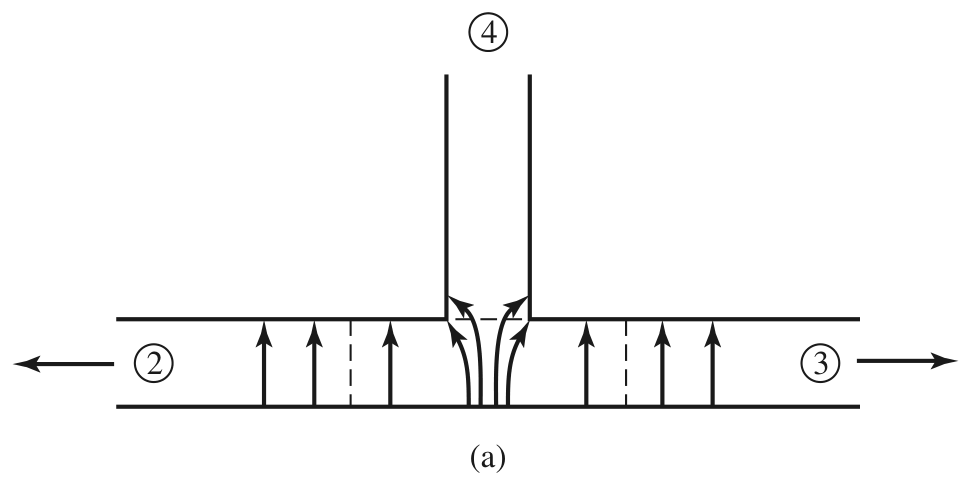
\includegraphics[width=0.49\linewidth]{figs/c3_magictee_a.png}\hfill
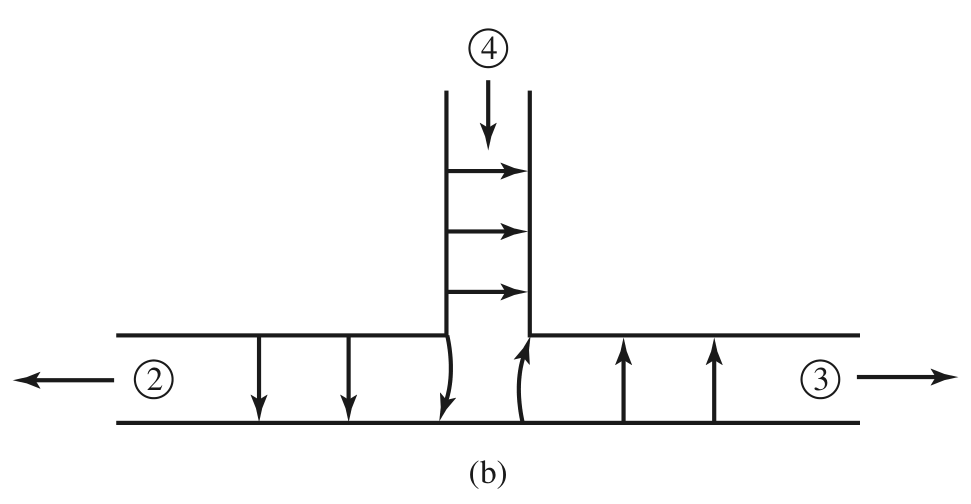
\includegraphics[width=0.49\linewidth]{figs/c3_magictee_b.png}}{%
\vspace{2pt}
{\color{sub}\scriptsize $E$ in the collinear arms (2), (3) of a magic tee.
(a) fed from the H-arm (Pozar's port 1, the sum port): the arms are driven \mk{in phase}, the
matching-sign column. (b) fed from the E-arm (4): \mk{antiphase}, the sign-flipped
column. Pozar numbers the arms differently from the papers, so label by E and H, not by number.
Pozar Fig 7.50.}}

\penalty0\vspace{2pt}

%=======================================================================
\T{4.7 Power Splitting and Combining: the Radar Questions}

\Q{Two identical radar transmitters must deliver twice the power to one antenna; and an ASR needs half the transmitter power at the antenna through a duplexer. Solve both with an S-matrix}{\m{6}\m{8}\m{10}}
{\color{sub}\footnotesize \tF{4} \yr{73 Ma, \textbf{73 Bh}, 74 Ma, \textbf{76 Bh}} \gap$\cdot$\gap \mk{one device, two directions: the magic tee combines and splits}}

\sbs{%
\lead{Combining: two transmitters into one antenna}
\begin{itemize}
  \item \textbf{Device}: magic tee (or a $3$ dB hybrid coupler).
  \item \textbf{Connection}: the two transmitters drive the collinear arms 1 and 2
    \textbf{in phase and at equal amplitude}; the antenna hangs on the H-arm (port 4);
    the E-arm (port 3) carries a \textbf{matched dummy load}.
  \item \textbf{S-matrix} of the magic tee ($\S$4.5; collinear 1, 2, E-arm 3, H-arm 4):
    \[ [S] = \tfrac{1}{\sqrt{2}}\begin{bmatrix} 0&0&1&1 \\ 0&0&-1&1 \\ 1&-1&0&0 \\ 1&1&0&0
       \end{bmatrix} \]
  \item \textbf{Drive vector}: equal amplitude, in phase, so $a_1 = a_2 = a$ and
    $a_3 = a_4 = 0$.
  \item \textbf{Multiply out}, $[b] = [S][a]$:
    \[ \begin{bmatrix} b_1\\ b_2\\ b_3\\ b_4 \end{bmatrix}
       = \tfrac{1}{\sqrt{2}}\begin{bmatrix} 0&0&1&1 \\ 0&0&-1&1 \\ 1&-1&0&0 \\ 1&1&0&0
         \end{bmatrix}\begin{bmatrix} a\\ a\\ 0\\ 0 \end{bmatrix}
       = \begin{bmatrix} 0\\ 0\\ 0\\ \sqrt{2}\,a \end{bmatrix} \]
\end{itemize}}{%
\lead{Combining: reading the answer off $[b]$}
\begin{itemize}
  \item \textbf{Read each row}: $b_4 = \tfrac{1}{\sqrt{2}}(a_1 + a_2)$, the sum at the
    H-arm; $b_3 = \tfrac{1}{\sqrt{2}}(a_1 - a_2) = 0$, the difference at the E-arm;
    $b_1 = b_2 = 0$ because $S_{11} = S_{22} = S_{12} = 0$.
  \item \textbf{Powers}, with $P = |a|^2$ per transmitter:
    \[ |b_4|^2 = 2|a|^2 = 2P, \qquad |b_1|^2 = |b_2|^2 = |b_3|^2 = 0 \]
  \item \textbf{Result}: the antenna receives $2P$, twice what either transmitter can
    deliver; the dummy load receives nothing, and nothing reflects back into either
    transmitter. Power in $2P$ = power out $2P$: lossless.
  \item \textbf{Why the tee and not a plain T-junction}: $S_{12} = 0$, so the two
    transmitters are \textbf{isolated} and cannot pull or damage each other; and all four
    ports stay matched, so neither transmitter sees a VSWR.
  \item \textbf{Practical riders} worth a mark each:
  \begin{itemize}
    \item Phase must be equalised, so the two feed lines are cut to the same electrical
      length.
    \item Amplitude imbalance $\Delta$ shows up as $|b_3|^2 \neq 0$: the dummy load
      absorbs exactly the mismatch, which is what protects the transmitters.
    \item The dummy load must be rated for the full unbalanced power.
  \end{itemize}
\end{itemize}}

\penalty0\vspace{3pt}
\sbs{%
\lead{Splitting: half the transmitter power to the antenna}
\begin{itemize}
  \item \textbf{Device}: the same magic tee, used as a duplexer, driven from the H-arm.
  \item \textbf{Connection}: transmitter on port 4 (H-arm), antenna on port 1, matched
    load on port 2, receiver on port 3 (E-arm).
  \item \textbf{S-matrix of the duplexer}, which is what \textbf{76 Bh} asks you to
    prepare: the magic tee's, with rows and columns in the order
    (1 Ant, 2 Load, 3 Rx, 4 Tx):
    \[ [S] = \tfrac{1}{\sqrt{2}}\begin{bmatrix} 0&0&1&1 \\ 0&0&-1&1 \\ 1&-1&0&0 \\ 1&1&0&0
       \end{bmatrix} \]
  \item \textbf{Transmit}, $a_4 = a$ and all other inputs zero:
    \[ \begin{bmatrix} b_1\\ b_2\\ b_3\\ b_4 \end{bmatrix}
       = \tfrac{1}{\sqrt{2}}\begin{bmatrix} 0&0&1&1 \\ 0&0&-1&1 \\ 1&-1&0&0 \\ 1&1&0&0
         \end{bmatrix}\begin{bmatrix} 0\\ 0\\ 0\\ a \end{bmatrix}
       = \tfrac{1}{\sqrt{2}}\begin{bmatrix} a\\ a\\ 0\\ 0 \end{bmatrix} \]
    \[ |b_1|^2 = |b_2|^2 = \tfrac{1}{2}|a|^2, \qquad |b_3|^2 = |b_4|^2 = 0 \]
  \item \textbf{Result}: the antenna gets exactly $P/2$, as \textbf{76 Bh} requires, the
    load takes the other $P/2$, and the receiver gets \textbf{none} of the transmitter
    power ($S_{34} = 0$), which is the whole point of a duplexer.
\end{itemize}}{%
\lead{Splitting: the receive path}
\begin{itemize}
  \item \textbf{Receive}, echo $a_1 = e$ and all other inputs zero:
    \[ [b] = \tfrac{1}{\sqrt{2}}\begin{bmatrix} 0\\ 0\\ e\\ e \end{bmatrix}
       \;\Rightarrow\; |b_3|^2 = \tfrac{1}{2}|e|^2 \text{ to the receiver} \]
    The other half goes back to the transmitter. The $3$ dB penalty in each direction is
    the price of the magic-tee duplexer, and naming it shows you understand the device
    rather than reciting it.
  \item \textbf{Better answer for a real ASR}: a \textbf{ferrite circulator} duplexer
    routes the full power $1 \rightarrow 2$ and the full echo $2 \rightarrow 3$ with no
    $3$ dB loss. Quote it as the improvement whenever the question does not force the
    half-power split.
\end{itemize}
\lead{Answer skeleton for both}
\begin{itemize}
  \item Name the device, draw it with every arm labelled and every termination named.
  \item Write $[S]$ for the magic tee.
  \item Write the drive vector $[a]$ the connection creates.
  \item Multiply out, and read the answer off $|b|^2$.
  \item Close with the isolation and matching argument: that is the ``sufficient
    explanation'' the marks are for.
\end{itemize}}

\penalty0\vspace{3pt}
\sbsr{0.36}{%
\lead{The schematic to draw beside the tee}
\figT{c3_hybrid180.png}}{%
\vspace{2pt}
\begin{itemize}
  \item A magic tee is a $180^\circ$ hybrid: \mk{sum} port $\Sigma$ (the H-arm) and
    \mk{difference} port $\Delta$ (the E-arm), with outputs (2) and (3).
  \item \textbf{Combining}: equal in-phase inputs at (2), (3) add at
    $\Sigma$ and cancel at $\Delta$, so the dummy load on $\Delta$ sees nothing.
  \item \textbf{Splitting}: drive $\Sigma$ and (2), (3) each get half,
    in phase; $\Delta$ stays isolated.
  \item Pozar Fig 7.41.
\end{itemize}}

\penalty0\vspace{2pt}

\penalty0\vspace{2pt}

%=======================================================================
\T{4.8 Directional Couplers}

\Q{Explain directional couplers and the four parameters used to describe their performance}{\m{4}\m{5}\m{6}}
{\color{sub}\footnotesize \tF{3} \yr{\textbf{73 Bh}, \textbf{79 Ch}, \texttt{80 Ba}}}

\sbs{%
\lead{What it is}
\begin{itemize}
  \item A \textbf{4-port} junction that samples power travelling in \textbf{one direction}
    only.
  \item Main guide: port 1 (input) to port 2 (through).
  \item Auxiliary guide: port 4 (coupled) and port 3 (isolated), Gangaju's numbering.
  \item Ideal, all ports matched:
  \begin{itemize}
    \item $1 \rightarrow 2$ passes almost all the power.
    \item $1 \rightarrow 4$ a known small fraction.
    \item $1 \rightarrow 3$ nothing.
  \end{itemize}
  \item Uses: \textbf{power monitoring}, \textbf{reflectometers} and VSWR measurement
    (one coupler each way), network analysers, signal injection, and as a 3 dB hybrid.
  \item S-matrix: $\S$3.6. Note $\S$3.6 labels the coupled port 3; the numbering varies by
    text, the physics does not.
\end{itemize}}{%
\figT{c4_coupler.png}
{\color{sub}\scriptsize Block view, Gangaju slide 54.}
\lead{The four parameters ($P_i$ = power at port $i$, input at 1)}
\begin{tabularx}{\linewidth}{@{}L{1.6cm}L{2.7cm}X@{}}
\toprule
\hrow \thead{Parameter} & \thead{Definition} & \thead{Measures} \\
\midrule
Coupling $C$ & $10\log\dfrac{P_1}{P_4}$ dB & how much is sampled \\
Directivity $D$ & $10\log\dfrac{P_4}{P_3}$ dB & forward vs backward discrimination \\
Isolation $I$ & $10\log\dfrac{P_1}{P_3}$ dB & leakage to isolated port \\
Insertion loss & $10\log\dfrac{P_1}{P_2}$ dB & loss on the main line \\
\bottomrule
\end{tabularx}
\vspace{2pt}
\begin{itemize}
  \item $\boxed{I = C + D}$. Example: $P_1 = 10$ mW, $P_4 = 1$ mW, $P_3 = 0.1\,\mu$W
    $\Rightarrow C = 10$ dB, $D = 40$ dB, $I = 50$ dB.
  \item Good coupler: $D$ of 30 to 40 dB, VSWR near 1.
  \item \added{} \textbf{Frequency sensitivity} (coupling flatness): how far $C$ drifts
    over the specified band. A fifth figure some notes list; quote it after the four.
\end{itemize}}

\par\penalty0\Needspace{12\baselineskip}
\sbsr{0.42}{%
\figT{c4_twohole.png}
{\color{sub}\scriptsize Two-hole coupler, Gangaju slide 57.}}{%
\lead{Two-hole coupler: why it is directional}
\begin{itemize}
  \item Two small holes in the common wall, spaced $d = (2n+1)\lambda_g/4$.
  \item Each hole radiates a small wave into the auxiliary guide, both ways.
  \item \textbf{Forward} waves (towards port 4) travel equal total paths $\rightarrow$
    \textbf{in phase} $\rightarrow$ add.
  \item \textbf{Backward} waves (towards port 3) differ by $2d = (2n+1)\lambda_g/2$
    $\rightarrow$ $(2n+1)\pi$ out of phase $\rightarrow$ \textbf{cancel}.
  \item Exact only at one frequency; more holes with tapered sizes widen the band.
\end{itemize}}

\penalty0\vspace{2pt}

%=======================================================================
\T{4.9 Ferrite Devices: Circulators, Isolators, Phase Shifters}

\Q{Explain the microwave circulator}{\m{5}}
{\color{sub}\footnotesize \tF{3} \yr{\textbf{70 Bh}, \textbf{72 Ash}, 73 Ma} \gap$\cdot$\gap asked word for word each time}

\sbs{%
\lead{Circulator}
\begin{itemize}
  \item A \textbf{non-reciprocal} multi-port in which power entering port $n$ leaves only
    by port $n+1$: $1 \rightarrow 2 \rightarrow 3 \rightarrow 1$ (3-port), or round four
    ports.
  \item Ideal: \textbf{matched} at every port and \textbf{lossless}, but $S_{ij} \ne S_{ji}$.
    3-port form (matrix of $\S$3.5):
    $[S] = \left[\begin{smallmatrix}0&0&1\\1&0&0\\0&1&0\end{smallmatrix}\right]$.
  \item Non-reciprocity comes from a \textbf{magnetised ferrite}.
  \item \textbf{Faraday rotation}: a plane wave along a ferrite rod in an axial magnetic
    field has its polarisation rotated by an angle set by the field strength and the rod
    length, and in the \textbf{same absolute sense} whichever way it travels. A return trip
    therefore doubles the rotation instead of undoing it.
  \item \textbf{Four-port construction} (slide 62): two 3 dB side-hole couplers, a primary
    and a secondary guide, and a non-reciprocal ferrite phase shifter in each.
  \begin{itemize}
    \item Port 1 $\rightarrow$ port 2: both paths arrive with the same phase $\rightarrow$
      add.
    \item Port 1 $\rightarrow$ port 4: the paths differ by 180$^\circ$ $\rightarrow$ cancel.
    \item The phase shifters behave differently in the reverse direction, so port 2 feeds
      port 3, port 3 feeds 4, port 4 feeds 1.
  \end{itemize}
\end{itemize}}{%
\figT{c4_circulator.png}
{\color{sub}\scriptsize Four-port circulator: two 3 dB couplers plus ferrite phase shifters.
Gangaju slide 62.}
\lead{Applications}
\begin{itemize}
  \item \textbf{Duplexer}: transmitter port 1, antenna 2, receiver 3 ($\S$4.5).
  \item Reflection amplifiers (tunnel diode, parametric): separate input from output.
  \item An \textbf{isolator}, by loading one port.
\end{itemize}
\lead{Isolator (uniline)}
\begin{itemize}
  \item Passes power one way, \textbf{absorbs} it the other way:
    $[S] = \left[\begin{smallmatrix}0&0\\1&0\end{smallmatrix}\right]$.
  \item Circulator with port 3 matched-terminated, or a Faraday-rotation isolator:
  \begin{itemize}
    \item Input E vertical; ferrite rotates it $45^\circ$; output guide twisted
      $45^\circ$ to accept it.
    \item Reflection from the load is rotated a further $45^\circ$ in the same sense
      $\rightarrow$ $90^\circ$ from the input orientation $\rightarrow$ absorbed by a
      resistive vane.
  \end{itemize}
  \item Use: between a klystron or magnetron and its load, so a mismatch cannot reflect
    back and pull the oscillator frequency.
\end{itemize}
\figT{c4_isolator.png}}

\par\penalty0\Needspace{9\baselineskip}
\lead{Phase shifter (syllabus, not yet asked)}
\begin{itemize}
  \item Changes the phase of the transmitted wave by $\Delta\phi = 2\pi l/\lambda_g$,
    either by changing the \textbf{length} $l$ or the \textbf{guide wavelength} $\lambda_g$.
  \item Mechanical: telescoping coaxial line; \textbf{dielectric vane} moved across the
    guide (more dielectric in the high-E centre, smaller $\lambda_g$, more phase).
  \item Electrical: \textbf{ferrite} under a variable bias field; PIN-diode switched lines.
  \item Uses: phased-array beam steering, phase discriminators, power-amplifier
    linearisation.
\end{itemize}

\penalty0\vspace{2pt}

%=======================================================================
\T{4.10 Cavity Resonators}

\Q{Explain microwave cavity resonators}{\m{4}\m{6}}
{\color{sub}\footnotesize \tP{2} \yr{74 Ma, \textbf{74 Bh}}}

\sbsr{0.58}{%
\lead{What and why}
\begin{itemize}
  \item A closed metal enclosure that stores EM energy at discrete resonant frequencies:
    a section of waveguide shorted at \textbf{both} ends.
  \item Microwave replacement for the LC tank: lumped L and C fail above a few hundred MHz
    (radiation, skin effect, lead parasitics).
  \item Circuit analogue: stored E energy $\rightarrow$ C, stored H energy $\rightarrow$ L,
    wall loss $\rightarrow$ R.
  \item Types: \textbf{rectangular}, \textbf{circular}, \textbf{re-entrant} (the klystron
    cavity, Ch 5).
  \item Infinitely many modes; the lowest is the \textbf{dominant} mode.
\end{itemize}}{%
\figT{c4_rect_cavity.png}
{\color{sub}\scriptsize Rectangular cavity $a \times b \times d$. Gangaju slide 90.}}

\sbs{%
\lead{Rectangular cavity: resonant frequency}
\begin{itemize}
  \item Standing wave along $z$: the guide length must hold $p$ half guide-wavelengths,
    $d = p\lambda_g/2 \Rightarrow \beta = p\pi/d$.
  \item $k^2 = k_c^2 + \beta^2$ gives
    \[ f_{mnp} = \frac{1}{2\sqrt{\mu\epsilon}}\sqrt{\left(\frac{m}{a}\right)^2 + \left(\frac{n}{b}\right)^2 + \left(\frac{p}{d}\right)^2} \]
  \item Allowed indices:
  \begin{itemize}
    \item TE$_{mnp}$: $p \ge 1$, $m$ and $n$ not both zero.
    \item TM$_{mnp}$: $m, n \ge 1$, $p \ge 0$.
  \end{itemize}
  \item Dominant for $b < a < d$: \mk{TE$_{101}$},
    $f_{101} = \frac{c}{2}\sqrt{\frac{1}{a^2} + \frac{1}{d^2}}$.
    Example $2 \times 1 \times 3$ cm: $9.01$ GHz, next TE$_{102}$ at $12.5$ GHz.
  \item Circular cavity, radius $a$, length $d$:
    $f = \dfrac{c}{2\pi}\sqrt{\left(\dfrac{p'_{nm}}{a}\right)^2 + \left(\dfrac{l\pi}{d}\right)^2}$
    (TE), with $p_{nm}$ for TM.
\end{itemize}}{%
\lead{Quality factor}
\begin{itemize}
  \item $Q = \omega\,\dfrac{\text{energy stored}}{\text{power lost}}$.
  \item Cavities reach $10^4$ to $10^6$; a lumped LC circuit about $10^2$.
  \item Losses add as reciprocals:
    \[ \frac{1}{Q_L} = \frac{1}{Q_c} + \frac{1}{Q_d} + \frac{1}{Q_{ext}} \]
  \begin{itemize}
    \item $Q_c$: wall conduction loss.
    \item $Q_d = 1/\tan\delta$: dielectric filling.
    \item $Q_{ext}$: power taken by the coupling; $Q_L$ is the loaded Q.
  \end{itemize}
  \item Coupling (probe, loop, aperture) is \textbf{under-}, \textbf{critically} or
    \textbf{over-coupled}; at critical coupling the input is matched.
\end{itemize}
\lead{Applications}
\begin{itemize}
  \item Klystron and magnetron cavities; wavemeters; filters; oscillator stabilisation;
    TR cells in duplexers.
\end{itemize}
\lead{\added{} Tuning a cavity}
\begin{itemize}
  \item Change the stored field and $f_0$ moves: a \textbf{plunger} alters the length $d$;
    a \textbf{post or screw} inserted where E is strongest adds capacitance and lowers
    $f_0$ (\textbf{capacitive} tuning); one where H is strongest reduces the
    inductance and \textbf{raises} $f_0$ (\textbf{inductive} tuning).
  \item Used to set the resonant frequency, match the cavity to its line and trim $Q$.
\end{itemize}}

\penalty0\vspace{2pt}

%=======================================================================
\T{4.11 Solid-State and Quantum Devices: Gunn Diode, MASER, Microwave Transistors}

\Q{Gunn diode}{\m{4}}
{\color{sub}\footnotesize \tP{1} \yr{\textbf{\texttt{79 Bh}}} \gap$\cdot$\gap short note}

\sbsr{0.56}{%
\begin{itemize}
  \item \textbf{Transferred-electron device (TED)}: bulk n-type GaAs (or InP), \textbf{no
    p-n junction}; ``diode'' only because it has two terminals.
  \item \textbf{Construction}: n$^+$ contact / lightly doped n active layer (epitaxial,
    about 6 to 18 $\mu$m) / n$^+$ substrate, metal contacts, heat sink.
  \item \textbf{Two-valley model} (Ridley-Watkins-Hilsum):
  \begin{itemize}
    \item GaAs conduction band has a \textbf{lower valley} (light electrons, high mobility)
      and an \textbf{upper satellite valley} about $0.36$ eV higher (heavy, low mobility).
    \item Low field: electrons stay in the lower valley, current rises with voltage.
    \item Above a threshold field (about $3.2$ kV/cm) electrons gain enough energy to
      \textbf{transfer} to the upper valley $\rightarrow$ average mobility falls
      $\rightarrow$ drift velocity \textbf{falls as field rises}.
    \item That is \textbf{negative differential resistance} between the peak and the valley
      of the I-V curve.
  \end{itemize}
  \item \textbf{Oscillation}: a high-field \textbf{domain} forms at the cathode, drifts to
    the anode at $v_d \approx 10^5$ m/s, and a new one forms when it arrives:
    \[ f = \frac{v_d}{L} \quad\text{e.g. } \frac{10^5}{10\,\mu\text{m}} = 10\ \text{GHz} \]
  \item \textbf{Correction to the deck} (slide 72): it says the low-field current rises
    because electrons move from the valence band to the conduction band. It does not; the
    carriers are already conduction electrons in the lower valley. \added{}
\end{itemize}}{%
\figT{c4_gunn_build.png}
\vspace{2pt}

\figT{c4_gunn_iv.png}
{\color{sub}\scriptsize Construction and the peak-valley characteristic. Gangaju slides 69 and
73.}
\lead{(+) and (-)}
\begin{itemize}
  \item (+) small, cheap, low noise, wide band, reliable, 1 to 100+ GHz.
  \item (-) low efficiency (a few \%), poor temperature stability, high bias current.
\end{itemize}
\lead{Applications}
\begin{itemize}
  \item Local oscillators, police and door-opening radar sensors, low-power transmitters,
    microwave relay links.
\end{itemize}}

\par\penalty0\Needspace{14\baselineskip}
\Q{MASER}{\m{4}}
{\color{sub}\footnotesize \tP{1} \yr{\texttt{80 Ba}} \gap$\cdot$\gap short note}

\sbsr{0.64}{%
\begin{itemize}
  \item \textbf{M}icrowave \textbf{A}mplification by \textbf{S}timulated \textbf{E}mission of
    \textbf{R}adiation: the microwave ancestor of the laser (Townes, 1954).
  \item A \textbf{quantum} device working on energy levels of atoms or molecules. The deck's
    ``semiconductor device'' is wrong. \added{}
  \item \textbf{Three-level principle}:
  \begin{itemize}
    \item \textbf{Pump} at $f_{13}$ lifts particles from level 1 to 3.
    \item They decay without radiating to the \textbf{metastable} level 2 and accumulate
      $\rightarrow$ \textbf{population inversion} between 2 and 1.
    \item An incoming signal at $f_{21} = (E_2 - E_1)/h$ \textbf{stimulates} emission of
      identical photons (same frequency, phase, direction) $\rightarrow$ coherent
      \textbf{amplification}.
  \end{itemize}
  \item \textbf{Types}: ammonia gas maser (23.87 GHz, the first), hydrogen maser
    (1.42 GHz, frequency standard), solid-state ruby maser (Cr$^{3+}$ in Al$_2$O$_3$,
    tuned by a magnetic field, cooled to a few kelvin).
  \item \textbf{Key property}: extremely \textbf{low noise}.
  \item \textbf{Applications}: radio-telescope and deep-space receivers, satellite ground
    stations, atomic clocks.
\end{itemize}}{%
\figT{c4_maser.png}
{\color{sub}\scriptsize Pump to level 3, relax to 2, stimulated transition 2 to 1. Gangaju slide
78.}}

\par\penalty0\Needspace{12\baselineskip}
\lead{Microwave transistors (syllabus, not yet asked)}
\sbs{%
\begin{itemize}
  \item Differ from low-frequency parts in \textbf{geometry} and \textbf{packaging}:
    interdigitated, overlay and matrix layouts cut lead inductance and junction capacitance.
  \item \textbf{Si BJT}: up to a few GHz. \textbf{HBT} (heterojunction, e.g. SiGe,
    InGaP/GaAs): higher $f_T$, amplifiers and MMICs.
  \item \textbf{GaAs MESFET}: Schottky-barrier gate on an n-channel; high electron mobility
    $\rightarrow$ well above 5 GHz; low noise, depletion-mode.
  \item \textbf{HEMT}: AlGaAs/GaAs heterojunction confines a 2-D electron gas in undoped
    GaAs, away from donor scattering $\rightarrow$ even higher mobility, beyond 20 GHz,
    lowest noise.
\end{itemize}}{%
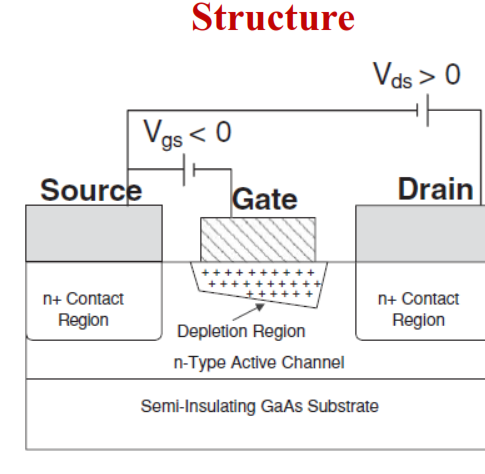
\includegraphics[width=0.48\linewidth]{figs/c4_mesfet.png}\hfill
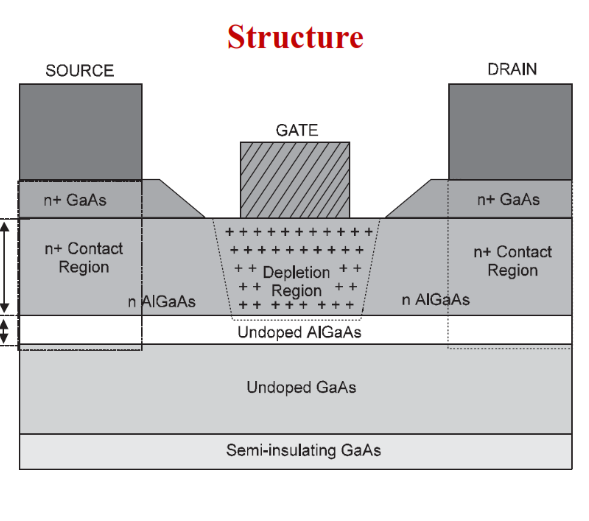
\includegraphics[width=0.48\linewidth]{figs/c4_hemt.png}
{\color{sub}\scriptsize MESFET (left) and HEMT (right) cross-sections. Gangaju slides 85 and 86.}}

\penalty0\vspace{2pt}

%=======================================================================
\T{4.12 Attenuators, Terminations, Windows, Microstrip}

\Q{Microstrips}{\m{5}}
{\color{sub}\footnotesize \tP{1} \yr{\textbf{69 Bh}} \gap$\cdot$\gap geometry and microstrip vs strip-line are in $\S$1.6; stub realisation in $\S$2.9}
\begin{itemize}
  \item Strip of width $W$ on a substrate of thickness $h$ and permittivity $\epsilon_r$,
    ground plane underneath, air above.
  \item \textbf{Quasi-TEM}: the field lives partly in air and partly in the substrate, so it
    sees an effective permittivity
    $\epsilon_{\text{eff}} = \dfrac{\epsilon_r + 1}{2} + \dfrac{\epsilon_r - 1}{2}\dfrac{1}{\sqrt{1 + 12h/W}}$,
    $1 < \epsilon_{\text{eff}} < \epsilon_r$.
  \item $v_p = c/\sqrt{\epsilon_{\text{eff}}}$, $\lambda_g = \lambda_0/\sqrt{\epsilon_{\text{eff}}}$;
    $Z_0$ falls as $W/h$ rises.
  \item (+) planar, cheap photolithography, components mount on top, MMIC friendly.
  \item (-) radiation at bends, dispersion, lower Q and power than waveguide, crosstalk.
\end{itemize}

\par\penalty0\Needspace{14\baselineskip}
\sbsr{0.58}{%
\lead{Attenuators and terminations (syllabus, not yet asked)}
\begin{itemize}
  \item \textbf{Attenuator}: reduces power by a set amount with low VSWR; a resistive
    (carbon) vane or flap in the guide absorbs power through induced currents.
  \begin{itemize}
    \item \textbf{Fixed}: lossy vane, or lossy walls.
    \item \textbf{Variable}: \textbf{flap} lowered through a slot in the centre of the
      broad wall (deeper $=$ more loss, since E is strongest there), \textbf{vane} moved
      from side wall to centre, or \textbf{rotary} vane in a circular guide.
  \end{itemize}
  \item \textbf{Matched termination}: absorbs all incident power; a guide section ending in
    a \textbf{tapered} absorbing wedge so the impedance changes gradually and nothing
    reflects.
  \item Reference \textbf{short}: a metal plate; \textbf{sliding short}: movable, sets a
    reactance.
\end{itemize}}{%
\figT{c4_attenuator.png}
{\color{sub}\scriptsize Flap and rotating-vane attenuators. Gangaju slide 39.}
\lead{Windows, posts and screws (waveguide matching)}
\begin{itemize}
  \item \textbf{Inductive window}: diaphragms from the \textbf{side} walls $\rightarrow$
    shunt L.
  \item \textbf{Capacitive window}: from \textbf{top and bottom} $\rightarrow$ shunt C;
    limits power (breakdown).
  \item \textbf{Resonant window}: both $\rightarrow$ parallel LC, transparent at resonance.
  \item \textbf{Post / screw}: part-way in $\rightarrow$ capacitive; right through
    $\rightarrow$ inductive; $\lambda/4$ deep $\rightarrow$ series resonance.
  \item Waveguide equivalent of a stub ($\S$2.6).
\end{itemize}}

\penalty0\vspace{2pt}

%=======================================================================
\T{4.13 PYQ Mapping}

\lead{Theory questions, covered in this document}
\begin{itemize}
  \item \textbf{Rectangular waveguide field equations, TE mode} $\rightarrow$ $\S$4.1.
    \yr{\textbf{70 Bh} \m{7}, 74 Ma \m{4}, \textbf{77 Ch} \m{8}, \textbf{79 Ch} \m{10},
    \textbf{80 Ch} \m{10}, \textbf{\texttt{80 Bh}} \m{4}}
  \item \textbf{Rectangular waveguide field equations, TM mode} $\rightarrow$ $\S$4.1.
    \mk{Most repeated topic of the chapter, with the TE list: 14 papers.}
    \yr{70 Ma \m{7}, \textbf{71 Bh} \m{8}, 72 Ma \m{5}, \textbf{74 Bh} \m{10},
    \textbf{76 Bh} \m{10}, \texttt{81 Ba} \m{8}, \textbf{\texttt{81 Bh}} \m{8}}
  \item \textbf{Rectangular waveguide: modes of propagation and critical parameters}
    $\rightarrow$ $\S$4.1 Step 7 and $\S$4.2. \yr{\textbf{69 Bh} \m{8}}
  \item \textbf{Prove TM$_{01}$ / TM$_{10}$ do not exist} $\rightarrow$ $\S$4.2. \yr{70 Ma \m{3}}
  \item \textbf{Lowest TM mode is TM$_{11}$} $\rightarrow$ $\S$4.2. \yr{\textbf{\texttt{82 Bh}} \m{3}}
  \item \textbf{TE$_{10}$ dominant; TE$_{10}$ vs TE$_{20}$} $\rightarrow$ $\S$4.2, with the
    81 Bh inequality defect. \yr{\textbf{71 Bh} \m{2}, \textbf{\texttt{81 Bh}} \m{3}}
  \item \textbf{Dominant and degenerate modes; $a = 3b$} $\rightarrow$ $\S$4.2 and
    companion Problem 4. \yr{\textbf{72 Ash} \m{5}, 72 Ma \m{2+2}, \texttt{82 Ba} \m{3}}
  \item \textbf{Circular waveguide, TE / TM field equations, TE vs TM, dominant mode}
    $\rightarrow$ $\S$4.3. \yr{71 Ma \m{10}, \textbf{75 Bh} \m{8+2}, \textbf{\texttt{79 Bh}} \m{10},
    \texttt{82 Ba} \m{7}}
  \item \textbf{Probe vs loop coupling} $\rightarrow$ $\S$4.4. \yr{\textbf{69 Bh} \m{5}}
  \item \textbf{Magic tee: principle, S-parameters, derivation} $\rightarrow$ $\S$4.5 and
    companion Problem 8. \yr{71 Ma \m{5}, \textbf{71 Bh} \m{5}, \textbf{72 Ash} \m{3+3}, 72 Ma \m{6},
    \textbf{79 Ch} \m{5}, \textbf{\texttt{79 Bh}} \m{4}, \textbf{80 Ch} \m{5},
    \textbf{\texttt{80 Bh}} \m{4}}
  \item \textbf{Magic tee with both arms shorted} $\rightarrow$ $\S$4.5 and companion
    Problem 12. \added{} \yr{\textbf{\texttt{82 Bh}} \m{4}}
  \item \textbf{S-matrices of E-plane tee, H-plane tee and a duplexer, and their uses}
    $\rightarrow$ $\S$4.5 and companion Problems 6 and 7. \yr{\texttt{81 Ba} \m{8}}
  \item \textbf{E-plane vs H-plane tee} $\rightarrow$ $\S$4.5. \yr{\textbf{69 Bh} \m{5}, \texttt{80 Ba} \m{4}}
  \item \textbf{Hybrid tee; terminated E, H, co-planar arms} $\rightarrow$ $\S$4.5 and
    companion Problem 11. \yr{70 Ma \m{8}, \texttt{82 Ba} \m{4+4+2}}
  \item \textbf{Two magic tees joined at E-arms / in H-plane} $\rightarrow$ $\S$4.5 and
    companion Problems 9 and 10. \yr{\textbf{77 Ch} \m{10}, \textbf{78 Ch} \m{5}}
  \item \textbf{Identify the passive device from a printed S-matrix} $\rightarrow$
    $\S$4.6 and companion Problems 13 to 15, all three printed matrices worked.
    \yr{\textbf{74 Bh} \m{8}, \textbf{75 Bh} \m{6}, \textbf{78 Ch} \m{10},
    \textbf{\texttt{81 Bh}} \m{5}}
  \item \textbf{Radar power combining and duplexer power splitting} $\rightarrow$ $\S$4.7
    and companion Problems 16 and 17.
    \yr{73 Ma \m{8}, \textbf{73 Bh} \m{8}, 74 Ma \m{6}, \textbf{76 Bh} \m{10}}
  \item \textbf{3-port directional coupler, S-parameter analysis} $\rightarrow$ $\S$4.5,
    $\S$3.5. \yr{\textbf{75 Bh} \m{4}}
  \item \textbf{Directional couplers; four performance parameters} $\rightarrow$ $\S$4.8.
    \yr{\textbf{73 Bh} \m{6}, \textbf{79 Ch} \m{5}, \texttt{80 Ba} \m{4}}
  \item \textbf{Circulators} $\rightarrow$ $\S$4.9. \yr{\textbf{70 Bh} \m{5}, \textbf{72 Ash} \m{5}, 73 Ma \m{5}}
  \item \textbf{Cavity resonators} $\rightarrow$ $\S$4.10. \yr{74 Ma \m{4}, \textbf{74 Bh} \m{6}}
  \item \textbf{Gunn diode} $\rightarrow$ $\S$4.11. \yr{\textbf{\texttt{79 Bh}} \m{4}}
  \item \textbf{MASER} $\rightarrow$ $\S$4.11. \yr{\texttt{80 Ba} \m{4}}
  \item \textbf{Microstrips} $\rightarrow$ $\S$4.12 and $\S$1.6. \yr{\textbf{69 Bh} \m{5}}
\end{itemize}

\lead{Numerical content}
\begin{itemize}
  \item \textbf{This chapter has a numerical companion}, \textit{Ch4 - RF Microwave Components
    and Devices - Numerical Problems and Solutions}: rectangular-guide parameters
    (\texttt{80 Ba}, 77 Ch), cut-off checks (70 Bh, \texttt{80 Bh}), mode ranking (72 Ma),
    circular-guide cut-offs (75 Bh), the E-plane, H-plane and magic-tee derivations,
    the junction problems (77 Ch, 78 Ch, \texttt{82 Ba}, \texttt{82 Bh}), the three
    device identifications and the two radar power problems.
\end{itemize}

\lead{Syllabus topics never asked in 24 papers}
\begin{itemize}
  \item Termination, phase shifter, attenuators, microwave transistor. Each has a short
    band above ($\S$4.9, $\S$4.11, $\S$4.12) sized for a 4-mark short note.
\end{itemize}

\lead{Errors in the sources, corrected here}
\begin{itemize}
  \item Deck slide 18: $k_y = n\pi/a$ should be $n\pi/b$.
  \item Deck slide 22: figure caption gives the wrong guide size (it is 5 cm $\times$ 2 cm).
  \item Deck slide 72: Gunn low-field current is not a valence-to-conduction transition.
  \item Deck slide 77: a MASER is a quantum device, not a semiconductor device.
  \item Waveguide.pdf p11: TM $E_\phi$ has a minus sign.
  \item Paper 81 Bh Q3a: TE$_{10}$ is dominant when $a > b$, not $b > a$.
\end{itemize}

\cleardoublepage
\section{Microwave Generators}
{\color{sub}\footnotesize 5 hrs \gap$\cdot$\gap asked in \mk{23 of 24 papers}
\gap$\cdot$\gap 5 syllabus sub-topics \gap$\cdot$\gap \mk{200 marks, 9.7\% of the archive}
$\rightarrow$ two tubes (klystron, magnetron) answer most of it; one idea (bunching) is the
2-mark rider on almost every question.}

\vspace{3pt}\noindent
\colorbox{gdL}{\makebox[\dimexpr\textwidth-2\fboxsep][l]{%
  \textcolor{gd}{\bfseries\footnotesize READ THIS FIRST}}}
\par\nobreak\vspace{3pt}

Chapter 5 is descriptive, with no numerical PYQ in 24 papers, and the questions come in a
fixed shape: \mk{a 2-mark definition, then a 6 to 8 mark ``construction and working''}.
\begin{enumerate}[label=\arabic*., leftmargin=1.4em, itemsep=1pt]
  \item \textbf{The 2-mark riders} (bunching, density modulation, transit time, cross-field
    effect, slow-wave structure) $\rightarrow$ each has a boxed two-line answer below.
    Bunching alone is asked in 9 papers.
  \item \textbf{Klystrons} (two-cavity, multicavity, reflex; 9 papers) $\rightarrow$
    $\S$5.3 and $\S$5.4. One figure (the Applegate diagram) explains all three.
  \item \textbf{Magnetron} (9 papers) $\rightarrow$ $\S$5.5. The ``45$^\circ$ / 60$^\circ$ /
    90$^\circ$ phase shift between adjacent cavities'' versions are the same answer plus
    one formula, $\phi = 2\pi n/N$.
\end{enumerate}
Two things worth knowing before the paper starts:
\begin{itemize}
  \item Every tube here does the same three things: \textbf{velocity-modulate} a beam,
    let it \textbf{bunch}, and \textbf{decelerate the bunches} in a field that takes their
    energy. Say this in the first line of any tube answer and the structure of the answer
    follows.
  \item Linear-beam (O-type) tubes: klystron, reflex klystron, TWT, BWO. Crossed-field
    (M-type) tubes: magnetron, crossed-field amplifier. An examiner who writes ``field
    effect'' or ``cross-field'' wants the M-type family.
\end{itemize}

\hr

%=======================================================================
\T{5.1 Conventional Tubes at Microwaves and the Transit-Time Effect}

\Q{How is the output of conventional tubes reduced at microwaves? What is transit-time effect?}{\m{2}\m{2+6}\m{2+8}}
{\color{sub}\footnotesize \tF{3} \yr{70 Ma, \textbf{77 Ch}, \textbf{\texttt{79 Bh}}} \gap$\cdot$\gap always the 2-mark opener to a tube question}

\sbsr{0.62}{%
\lead{Why triodes and pentodes fail above about 1 GHz}
\begin{itemize}
  \item \textbf{Inter-electrode capacitance} $C_{gp}, C_{gk}, C_{pk}$:
  \begin{itemize}
    \item Reactance $1/\omega C$ falls with frequency $\rightarrow$ shorts the input and
      output $\rightarrow$ gain falls.
    \item Cure (spread electrodes, smaller area) raises transit time: a
      \textbf{compromise}.
  \end{itemize}
  \item \textbf{Lead inductance}: $\omega L$ grows $\rightarrow$ degenerative feedback;
    cure: short leads (disk-seal tubes).
  \item \textbf{Transit-time effect} (below).
  \item \textbf{Cathode emission}: more current needs a bigger cathode, which adds
    capacitance; filament voltage and temperature are limited.
  \item \textbf{Power losses}: skin-effect resistance grows as $\sqrt{f}$; dielectric
    loss in the glass envelope; radiation from leads.
\end{itemize}}{%
\figT{c5_interelectrode.png}
{\color{sub}\scriptsize Inter-electrode capacitances of a triode. Karkee, Ch-5 deck, slide 4.}}

\par\penalty0\Needspace{11\baselineskip}
\creamq{Transit-time effect: the 2-mark answer}{\m{2}}
\begin{itemize}
  \item \textbf{Transit time} = time an electron takes from cathode to anode.
    \textbf{Transit-time effect}: when this becomes a significant fraction of one RF cycle,
    the grid voltage changes while the electron is in flight $\rightarrow$ plate current
    lags the grid voltage $\rightarrow$ efficiency and gain collapse.
  \item Numbers: $\tau = 1$ ns is $0.001$ cycle at 1 MHz but a \textbf{whole cycle} at
    1 GHz. Above about $0.1$ cycle the loss is serious.
  \item Estimate: 100 V gives $v = \sqrt{2eV/m} = 5.93\times10^6$ m/s; a 1 mm gap then takes
    $3.4\times10^{-10}$ s, i.e. $0.34$ cycle at 1 GHz.
  \item Cure in a conventional tube: closer electrodes and higher voltage (fights the
    capacitance). \mk{Cure in a microwave tube: exploit it.} Klystrons, TWTs and magnetrons
    turn transit time into velocity modulation and bunching.
\end{itemize}

\par\penalty0\Needspace{10\baselineskip}
\lead{\added{} The four effects solid-state generators exploit}
\begin{tabularx}{\linewidth}{@{}L{2.9cm}XL{2.6cm}@{}}
\toprule
\hrow \thead{Effect} & \thead{What happens} & \thead{Device} \\
\midrule
\textbf{Transit time} & Carrier drift across a region delays current behind voltage; a delay near half a cycle gives negative resistance & IMPATT, BARITT \\
\textbf{Tunnelling} & Carriers pass \textbf{through} a thin potential barrier they could not climb classically; current falls as bias rises past the peak & Tunnel diode \\
\textbf{Avalanche} & Strong field accelerates carriers until impact ionization knocks electrons out of covalent bonds, a chain reaction & IMPATT (with transit time) \\
\textbf{Transferred electron} (Gunn) & Above a threshold field (about 3.2 kV/cm in GaAs) electrons move to a low-mobility upper valley: negative differential mobility, no p-n junction & Gunn diode, $\S$4.11 \\
\bottomrule
\end{tabularx}

\penalty0\vspace{2pt}

%=======================================================================
\T{5.2 Velocity Modulation, Density Modulation and Bunching}

\Q{What is bunching effect (density modulation)? Explain velocity modulation and bunching}{\m{2}\m{5}\m{10}}
{\color{sub}\footnotesize \tS{9} \yr{\textbf{70 Bh}, \textbf{71 Bh}, \textbf{72 Ash}, 72 Ma, 73 Ma, \textbf{75 Bh}, \texttt{80 Ba}, \textbf{\texttt{80 Bh}}, \textbf{\texttt{81 Bh}}} \gap$\cdot$\gap \mk{the most repeated ask in the chapter}}

\colorbox{rowL}{\parbox{\dimexpr\linewidth-2\fboxsep}{\small
\textbf{2-mark answer.} \textbf{Velocity modulation}: an RF voltage across a gap speeds up
electrons crossing in one half-cycle and slows those crossing in the other. \textbf{Bunching}
(= \textbf{density modulation}): in the field-free drift space beyond, fast electrons catch
up with slow ones sent earlier, so the uniform beam gathers into \textbf{bunches} once per RF
cycle. The beam current is now modulated at the RF frequency and can drive a second cavity.}}

\par\penalty0\Needspace{20\baselineskip}
\sbsr{0.54}{%
\lead{The equations (for the 5 and 10 mark versions)}
\begin{itemize}
  \item Beam accelerated by $V_0$: $v_0 = \sqrt{2eV_0/m} = 0.593\times10^{6}\sqrt{V_0}$ m/s.
  \item Buncher gap voltage $V_1\sin\omega t$. Leaving at $t_1$:
    \[ v(t_1) = v_0\left[1 + \frac{\beta_i V_1}{2V_0}\sin\omega t_1\right] \]
    $\beta_i = \dfrac{\sin(\theta_g/2)}{\theta_g/2}$, the \textbf{beam coupling
    coefficient}; $\theta_g = \omega d/v_0$ the gap transit angle.
  \item Three reference electrons: \#2 crosses at zero voltage (unchanged), \#3 on the
    rising half (accelerated), \#1 before it (decelerated). \#1 and \#3 converge on \#2.
  \item Arrival at the catcher, drift length $L$: $t_2 = t_1 + L/v(t_1)$.
  \item \textbf{Bunching parameter}
    \[ X = \frac{\beta_i V_1}{2V_0}\,\theta_0, \qquad \theta_0 = \frac{\omega L}{v_0} \]
  \item Catcher current:
    $i_2 = I_0 + \sum_n 2I_0 J_n(nX)\cos n\omega(t_2 - \tau_0)$.
  \item Fundamental $2I_0 J_1(X)$ peaks at \mk{$X = 1.841$}, where it is $1.164\,I_0$
    $\rightarrow$ optimum drift length.
\end{itemize}}{%
\figT{c5_applegate.png}
{\color{sub}\scriptsize \textbf{Applegate diagram}: each line is one electron's distance vs
time; steep lines are fast. Lines converge (a bunch) around the electron that crossed at
zero gap voltage. Karkee deck, PDF p22.}
\vspace{2pt}
\begin{itemize}
  \item \textbf{Checked by simulation} in \code{tubes.py}: electrons launched with this
    velocity law and drifted ballistically give a fundamental of exactly $2J_1(X)$.
  \item Too short a drift ($X < 1.84$): weak bunches. Too long: electrons overtake and
    the bunch spreads again (\textbf{debunching}).
\end{itemize}}

\penalty0\vspace{2pt}

%=======================================================================
\T{5.3 Two-Cavity and Multicavity Klystrons}

\Q{Describe the construction and operation of a two-cavity / multicavity klystron amplifier or oscillator}{\m{4}\m{5}\m{2+7}\m{2+8}}
{\color{sub}\footnotesize \tS{7} \yr{\textbf{69 Bh}, 70 Ma, \textbf{71 Bh}, \textbf{72 Ash}, \textbf{78 Ch}, \textbf{80 Ch}, \texttt{82 Ba}} \gap$\cdot$\gap 70 Ma two-cavity; the rest mostly multicavity}

\sbsr{0.50}{%
\lead{Construction (two-cavity amplifier)}
\begin{itemize}
  \item \textbf{Electron gun}: heated cathode, focusing electrode, anode at $+V_0$ forms a
    narrow beam; an axial magnetic field keeps it focused.
  \item \textbf{Buncher cavity} (input): re-entrant cavity with grids across the beam; RF
    in via coaxial loop.
  \item \textbf{Drift space}: field-free tube of length $L$.
  \item \textbf{Catcher cavity} (output): identical cavity, RF out via loop.
  \item \textbf{Collector}: absorbs the spent beam.
  \item Cavities and collector at the same dc potential, so the beam drifts at constant
    mean speed.
\end{itemize}}{%
\figT{c5_twocavity.png}
{\color{sub}\scriptsize Two-cavity klystron. Karkee deck, slide 14.}}

\lead{Operation}
\begin{enumerate}[label=\arabic*., leftmargin=1.4em, itemsep=1pt]
  \item Weak RF in the buncher sets up $V_1\sin\omega t$ across its gap.
  \item \textbf{Velocity modulation}: electrons crossing are accelerated or decelerated
    ($\S$5.2).
  \item \textbf{Bunching} in the drift space: velocity modulation becomes density
    modulation.
  \item Bunches reach the catcher once per cycle and \textbf{induce} RF current in it. Its
    field builds up to \textbf{oppose} the bunches: they are decelerated and give up
    kinetic energy, while the thin stream between bunches is accelerated and takes back
    only a little.
  \item Net energy flows from beam to RF $\rightarrow$ amplified output. The beam leaves
    slower and is collected.
\end{enumerate}
\begin{itemize}
  \item \textbf{Correction to the source} (PDF p23): it says ``all the kinetic energy is
    converted''. Only part is; the beam still reaches the collector with most of its speed.
    Theoretical maximum efficiency is $\tfrac{1}{2}\times 1.164 = $ \mk{58\%} (at
    $X = 1.841$, catcher voltage equal to $V_0$); practical about 40\%. \added{}
  \item Gain of two cavities is low (about 10 dB) $\rightarrow$ multicavity.
\end{itemize}

\par\penalty0\Needspace{16\baselineskip}
\sbsr{0.34}{%
\figT{c5_threecavity.png}
{\color{sub}\scriptsize Multicavity klystron. Karkee deck, slide 19.}}{%
\lead{Multicavity klystron (amplifier)}
\begin{itemize}
  \item One or more \textbf{intermediate cavities} between buncher and catcher, not
    externally driven.
  \item Weak bunches from cavity 1 excite cavity 2 $\rightarrow$ its larger gap voltage
    re-modulates the beam $\rightarrow$ tighter bunches $\rightarrow$ and so on.
  \item Each stage adds gain: \textbf{30 to 70 dB} overall.
  \item \textbf{Stagger tuning} the cavities slightly apart widens the bandwidth.
  \item Higher efficiency and power: up to MW pulsed, kW CW.
  \item Uses: UHF TV and troposcatter transmitters, satellite ground stations, radar
    transmitters, linear accelerators.
\end{itemize}
\lead{Klystron oscillator}
\begin{itemize}
  \item Feed part of the catcher output \textbf{back} to the buncher with the right phase
    (feedback loop, slide 18) $\rightarrow$ self-sustained oscillation. Multicavity
    oscillator: the same loop around a multicavity tube (72 Ash).
  \item Tuned by the cavities; for a single-cavity, voltage-tuned oscillator use the reflex
    klystron ($\S$5.4).
\end{itemize}}

\penalty0\vspace{2pt}

%=======================================================================
\T{5.4 Reflex Klystron}

\Q{Explain velocity modulation and bunching in a reflex klystron with neat diagrams and equations}{\m{5}\m{10}}
{\color{sub}\footnotesize \tP{2} \yr{72 Ma, \textbf{75 Bh}} \gap$\cdot$\gap 75 Bh prints ``multicavity reflex klystron''; a reflex klystron has one cavity}

\sbsr{0.46}{%
\figT{c5_reflex.png}
{\color{sub}\scriptsize Karkee deck, PDF p29.}
\vspace{2pt}

\figT{c5_reflex_apple.png}
{\color{sub}\scriptsize Electrons $e_e, e_r, e_l$ return together: the bunch arrives
$n + \tfrac34$ cycles later. PDF p30.}}{%
\lead{Construction}
\begin{itemize}
  \item Electron gun, \textbf{one} re-entrant anode cavity at $+V_0$, and a
    \textbf{repeller} electrode at $-V_R$ beyond it.
  \item Output via a coaxial loop from the same cavity.
\end{itemize}
\lead{Operation}
\begin{enumerate}[label=\arabic*., leftmargin=1.4em, itemsep=1pt]
  \item Noise starts a small RF voltage across the cavity gap.
  \item Electrons crossing it are \textbf{velocity-modulated}.
  \item In the retarding repeller field they stop and turn back. A \textbf{faster}
    electron goes deeper and takes \textbf{longer}:
    round trip $T' = \dfrac{2mLv}{e(V_R + V_0)}$.
  \item So an early (fast) electron, the reference and a late (slow) one return
    \textbf{together}: the bunch forms in the \textbf{repeller space}.
  \item The bunch re-crosses the gap. If the gap field then opposes it, it gives energy
    to the cavity and oscillation grows.
\end{enumerate}
\lead{Condition for oscillation}
\begin{itemize}
  \item The bunch forms round the electron that left at zero gap voltage (going
    positive), and must return when the field most strongly retards it:
    \[ \boxed{T' = \left(n + \tfrac{3}{4}\right)\text{ cycles}}, \quad n = 0, 1, 2 \]
  \item Power returned to the gap $\propto -J_1(X)\sin\theta_0$: positive for
    $\theta_0$ in the second half-cycle, largest at $\tfrac34$. \code{tubes.py} scans
    $\theta_0$ with simulated electrons and finds the peak at $1.750$ cycles.
\end{itemize}}

\par\penalty0\Needspace{9\baselineskip}
\begin{itemize}
  \item \textbf{Electronic tuning}: changing $V_R$ changes $T'$ and pulls the frequency a
    few percent; modes are the different $n$.
  \item \textbf{Efficiency}: maximum $\dfrac{2X'J_1(X')}{2\pi n + 3\pi/2}$ with
    $X' = 2.405$: 53\% for $n = 0$ (not practical), \mk{22.7\% for $n = 1$}. The deck's
    22.78\% is this, with $X'$ rounded to 2.408. Practical 10 to 20\%.
  \item \textbf{Performance}: 4 to 200 GHz, 1 mW to 2.5 W. \textbf{Uses}: local oscillator
    in receivers, signal source for bench tests, portable links, pump for parametric
    amplifiers.
\end{itemize}

\penalty0\vspace{2pt}

%=======================================================================
\T{5.5 Cavity Magnetron and the Cross-Field Effect}

\Q{Describe the construction and working of a cavity magnetron; magnetron with 45 / 60 / 90 degree phase shift between adjacent cavities}{\m{5}\m{2+6}\m{8}\m{2+8}\m{10}}
{\color{sub}\footnotesize \tS{9} \yr{\textbf{70 Bh}, 71 Ma, 72 Ma, 74 Ma, \textbf{77 Ch}, \textbf{79 Ch}, \texttt{80 Ba}, \texttt{81 Ba}, \textbf{\texttt{81 Bh}}} \gap$\cdot$\gap 81 Bh's ``high-power oscillator using bunching and field effects'' is this tube}

\colorbox{rowL}{\parbox{\dimexpr\linewidth-2\fboxsep}{\small
\textbf{2-mark answer: cross-field effect} (72 Ma, 78 Ch, 81 Bh). An electron in
\textbf{perpendicular} dc electric and magnetic fields feels
$\vec F = -e(\vec E + \vec v\times\vec B)$. It does not go straight to the anode: it
follows a \textbf{cycloidal} path and drifts at $v = E/B$, perpendicular to both fields.
Crossed-field (M-type) tubes use this drift to keep electrons in step with an RF wave for a
long interaction.}}

\par\penalty0\Needspace{16\baselineskip}
\sbsr{0.50}{%
\lead{Construction}
\begin{itemize}
  \item Thick cylindrical \textbf{cathode} on the axis (radius $a$).
  \item Copper \textbf{anode block} (radius $b$) with $N$ (typically 8) \textbf{resonant
    cavities} cut into it, opening onto the \textbf{interaction space}.
  \item \textbf{Radial} dc field from anode voltage $V_0$; \textbf{axial} magnetic field
    from a permanent magnet, so $E \perp B$.
  \item Output: coupling loop in one cavity to a coaxial line or waveguide.
  \item \textbf{Straps} join alternate anode segments to hold the tube in the $\pi$-mode.
\end{itemize}}{%
\figT{c5_mag_build.png}
{\color{sub}\scriptsize Cavity magnetron cross-section and axial flux. PDF p55.}}

\par\penalty0\Needspace{16\baselineskip}
\sbsr{0.50}{%
\lead{Electron paths and the Hull cut-off}
\begin{itemize}
  \item $B = 0$: straight radial path to the anode.
  \item Small $B$: curved path, still reaches the anode.
  \item $B = B_c$: path just \textbf{grazes} the anode (cut-off).
  \item $B > B_c$: electron returns to the cathode without collecting.
  \item \textbf{Hull cut-off field}:
    \[ B_c = \frac{\sqrt{8mV_0/e}}{b\left(1 - a^2/b^2\right)} \]
  \item Checked by integrating electron trajectories in \code{tubes.py}: for
    $V_0 = 10$ kV, $a = 5$ mm, $b = 10$ mm the grazing field is $0.0899$ T, equal to the
    formula. \added{}
  \item The magnetron works just \textbf{above} $B_c$: without RF no electron reaches the
    anode.
\end{itemize}}{%
\figT{c5_mag_cutoff.png}
{\color{sub}\scriptsize (b) normal operation, (c) at cut-off. PDF p61.}
\vspace{2pt}

\figT{c5_mag_spokes.png}
{\color{sub}\scriptsize $\pi$-mode spoke pattern. Deck slide 50.}}

\par\penalty0\Needspace{14\baselineskip}
\lead{Operation (oscillator)}
\begin{enumerate}[label=\arabic*., leftmargin=1.4em, itemsep=1pt]
  \item Noise excites the cavities; RF fringing fields appear at the vane tips, alternating
    round the anode.
  \item Electrons circling the cathode meet these fields. Those in a \textbf{retarding}
    RF field slow down, feel less $v\times B$ force, and \textbf{drift outwards}, giving
    energy to the RF on the way.
  \item Those in an \textbf{accelerating} field curl back to the cathode (back-bombardment
    heats it, often enough to switch the heater off).
  \item The result is \textbf{phase focusing}: the electron cloud forms rotating
    \textbf{spokes}, each sitting in a retarding field. This is the magnetron's
    \textbf{bunching}.
  \item On the next half-cycle the field pattern reverses and the spokes rotate one cavity
    on, staying in step: sustained oscillation. Efficiency 40 to 70\%.
\end{enumerate}

\par\penalty0\Needspace{16\baselineskip}
\creamq{The phase-shift versions: 45, 60, 90 degrees between adjacent cavities}{\m{6+2}\m{8}\m{3+7}}
{\color{sub}\footnotesize \yr{74 Ma, \textbf{77 Ch}, \texttt{80 Ba} (45$^\circ$); \texttt{81 Ba} (60$^\circ$); 72 Ma (90$^\circ$)}}
\sbs{%
\begin{itemize}
  \item Around a ring of $N$ cavities the total phase must be a whole number of turns:
    \[ \phi = \frac{2\pi n}{N}, \quad n = 0, \pm1, \pm2 \text{ up to } \pm\frac{N}{2} \]
  \item $n = N/2$: $\phi = 180^\circ$, the \textbf{$\pi$-mode}, normal operation.
    $n = 0$: zero mode, no RF between anode and cathode, unused.
  \item The RF pattern repeats every $360^\circ/\phi$ cavities, so there is \textbf{one
    spoke} per that many cavities:
  \begin{itemize}
    \item $45^\circ$: 8 cavities per wavelength (in an 8-cavity tube $n = 1$, one spoke).
    \item $60^\circ$: 6 cavities per wavelength ($N = 6$, $n = 1$).
    \item $90^\circ$: 4 cavities per wavelength ($N = 8$ gives $n = 2$, two spokes).
    \item $180^\circ$: 2 cavities, $N/2$ spokes.
  \end{itemize}
\end{itemize}}{%
\begin{itemize}
  \item \textbf{Synchronism}: the spokes rotate at the RF pattern's angular velocity
    $\omega/n$; set $V_0$ and $B$ so the electron drift ($E/B$) matches it.
  \item \textbf{As a power amplifier} (80 Ba, 72 Ma): break the ring, feed RF in at one
    cavity and take it out several cavities later. The phase shift per cavity sets the
    wave's speed along the anode, $v_p = \omega p/\phi$ ($p$ = cavity pitch), and the
    beam drift is matched to it. That is the crossed-field amplifier of $\S$5.6.
  \item Write the sketch with the cavities marked $+$ / $-$ according to $\phi$ and draw
    the spokes in the retarding cavities; that sketch carries most of the marks.
  \item \textbf{Uses}: radar transmitters, microwave ovens (2.45 GHz), industrial heating,
    linear accelerators.
  \item \added{} \textbf{Frequency pushing}: a change in anode voltage changes the
    electron drift speed and so the oscillation frequency; cure, a regulated supply.
  \item \added{} \textbf{Frequency pulling}: a change in load impedance (antenna VSWR)
    reflects into the cavities and shifts the frequency; cure, an isolator or circulator
    between tube and load.
  \item \added{} \textbf{Pros}: high peak power (MW pulsed) from a small, efficient tube.
    \textbf{Cons}: noisy, poor frequency stability and control, so it is an oscillator,
    not a precision source.
\end{itemize}}

\penalty0\vspace{2pt}

%=======================================================================
\T{5.6 Crossed-Field Amplifier}

\Q{Explain the working principle of a circular-beam type microwave cavity-controlled crossed-field amplifier}{\m{3+7}\m{7}}
{\color{sub}\footnotesize \tP{2} \yr{72 Ma, \textbf{\texttt{82 Bh}}} \gap$\cdot$\gap the magnetron turned into an amplifier}

\sbsr{0.62}{%
\begin{itemize}
  \item A \textbf{crossed-field amplifier (CFA)}, also amplitron or platinotron: magnetron
    geometry, $E \perp B$, but with an RF \textbf{input} and an RF \textbf{output}.
  \item \textbf{Circular-beam (re-entrant beam)}: the electron stream circulates round the
    cathode continuously, as in a magnetron.
  \item \textbf{Cavity-controlled (non-re-entrant RF circuit)}: the anode cavities form a
    slow-wave line from input to output; between output and input sits an \textbf{RF
    absorber / insulator}, so the wave cannot circulate and the tube does not oscillate.
  \item \textbf{Working}:
  \begin{itemize}
    \item The input wave travels along the anode at $v_p = \omega p/\phi$.
    \item Electrons drift at $E/B$; matched to $v_p$ they \textbf{bunch into spokes} in
      the retarding phase of the wave ($\S$5.5).
    \item Spokes move with the wave and give up energy cavity by cavity $\rightarrow$ the
      wave grows $\rightarrow$ amplified output.
    \item Left-over electrons carry little RF past the absorber and re-enter the input
      region.
  \end{itemize}
  \item \textbf{Performance}: high efficiency (up to about 70\%), broad band (about 10\%),
    \textbf{low gain} (10 to 15 dB), high power.
  \item \textbf{Use}: final power stage of radar transmitters, driven by a TWT.
\end{itemize}}{%
\figT{c5_cfa.png}
{\color{sub}\scriptsize Circular CFA: input, output, absorber, spiralling electron flow.
Student presentation 2078.}}

\penalty0\vspace{2pt}

%=======================================================================
\T{5.7 Travelling Wave Tube}

\Q{Describe the construction and operation of a travelling wave tube (TWT)}{\m{2+6}}
{\color{sub}\footnotesize \tP{2} \yr{\textbf{\texttt{79 Bh}}, \textbf{\texttt{80 Bh}}}}

\sbsr{0.52}{%
\lead{Construction}
\begin{itemize}
  \item \textbf{Electron gun}: cathode, focusing plate, anode.
  \item \textbf{Helix}: a wire coil round the beam, the \textbf{slow-wave structure}; RF
    in at the gun end, out at the collector end.
  \item \textbf{Attenuator} midway along the helix: absorbs reflected waves so the tube
    cannot oscillate.
  \item \textbf{Focusing magnets} (solenoid or periodic permanent magnets) along the tube.
  \item \textbf{Collector}: collects the spent beam.
  \item \textbf{No resonant cavities} $\rightarrow$ very wide bandwidth.
\end{itemize}}{%
\figT{c5_twt.png}
{\color{sub}\scriptsize TWT construction. Student presentation 2078.}}

\lead{Operation}
\begin{enumerate}[label=\arabic*., leftmargin=1.4em, itemsep=1pt]
  \item RF on the helix travels round the turns at about $c$, but \textbf{along the axis}
    only at
    $v_p \approx c\,\dfrac{\text{pitch}}{2\pi r}$ (a few percent of $c$).
  \item The beam voltage is set so the electrons move slightly \textbf{faster} than $v_p$.
  \item The axial RF field velocity-modulates the beam $\rightarrow$ bunches form, and
    because beam and wave travel together the interaction lasts the \textbf{whole length}.
  \item Being slightly faster, the bunches sit in the retarding field and give energy to
    the wave, which grows exponentially $\rightarrow$ gain 30 to 60 dB.
\end{enumerate}
\begin{itemize}
  \item \textbf{Correction to the source} (PDF p38): the beam does \textbf{not} move at the
    velocity of light; the whole point of the helix is to slow the wave down to the beam.
    Example (\code{tubes.py}): pitch 1 mm, radius 2 mm gives $v_p = 0.079c$, matched by a
    beam of about 1.6 kV; a 1 kV beam moves at $0.063c$. \added{}
  \item \textbf{Performance}: 0.5 to 95 GHz, octave bandwidth, 5 to 20\% efficiency,
    mW to 10 MW pulsed. \textbf{Uses}: satellite transponders (long life), broadband
    receivers, radar, troposcatter links, EW jammers.
\end{itemize}
\par\penalty0\Needspace{9\baselineskip}
\begin{tabularx}{\linewidth}{@{}L{2.8cm}XX@{}}
\toprule
\hrow & \thead{Two-cavity klystron} & \thead{TWT} \\
\midrule
Interaction & at two gaps only & continuous, whole helix \\
RF circuit & resonant cavities & non-resonant slow-wave helix \\
Bandwidth & narrow (a few \%) & wide (an octave) \\
Wave & standing wave in cavities & travelling wave \\
Oscillation risk & needs feedback to oscillate & attenuator needed to prevent it \\
\bottomrule
\end{tabularx}

\penalty0\vspace{2pt}

%=======================================================================
\T{5.8 Backward Wave Oscillator and Slow-Wave Structures}

\Q{What is bunching effect? Explain the working principle of a BWO with neat diagrams}{\m{5}\m{2+8}}
{\color{sub}\footnotesize \tF{3} \yr{\textbf{71 Bh}, 73 Ma, \textbf{74 Bh}} \gap$\cdot$\gap 71 Bh and 74 Bh as short notes}

\sbsr{0.52}{%
\begin{itemize}
  \item \textbf{BWO} (carcinotron): a TWT-family tube used as an \textbf{oscillator},
    microwave up to terahertz.
  \item Electron gun, slow-wave structure (helix or folded line), collector, magnetic
    focusing. \textbf{No RF input}.
  \item The beam interacts with a \textbf{backward space harmonic}: its phase velocity is
    along the beam (so they stay in step) but its \textbf{group velocity}, the direction
    energy flows, is \textbf{towards the gun}.
  \item Bunches give energy to this wave; the energy travels back to the gun end, where it
    velocity-modulates newly arriving electrons: \textbf{built-in feedback} $\rightarrow$
    self-sustained oscillation.
  \item \textbf{Output is taken at the gun end}; the collector end is matched.
  \item \textbf{Frequency is tuned electronically} by the beam voltage (it sets which
    backward harmonic is in step): very wide tuning range.
  \item M-type BWO: crossed fields with a negative \textbf{sole} electrode (lower figure).
  \item Uses: swept signal generators, THz spectroscopy and imaging, jammers.
  \item \textbf{Not} a klystron: some student notes describe buncher and catcher cavities
    and a feedback conductor; a BWO has none.
\end{itemize}}{%
\figT{c5_bwo_helix.png}
{\color{sub}\scriptsize O-type BWO: output near the gun. Deck slide 40.}
\vspace{3pt}

\figT{c5_bwo_mtype.png}
{\color{sub}\scriptsize M-type BWO with sole. Student presentation 2078.}}

\par\penalty0\Needspace{8\baselineskip}
\creamq{What do you mean by a slow (backward) wave structure?}{\m{2}}
{\color{sub}\footnotesize \yr{\textbf{73 Bh}}}
\begin{itemize}
  \item A \textbf{slow-wave structure} is a periodic RF circuit that makes the wave's
    axial phase velocity much smaller than $c$, so an electron beam of practical voltage can
    keep in step with it: helix, folded-back line, ring-bar, interdigital line, coupled
    cavities.
  \item It is \textbf{backward} when the space harmonic used has phase and group velocity
    in \textbf{opposite} directions: energy flows against the beam, as the BWO needs.
\end{itemize}

\penalty0\vspace{2pt}

%=======================================================================
\T{5.9 Low-Noise Amplifier}

\Q{Explain the construction and working principle of an LNA}{\m{2+6}}
{\color{sub}\footnotesize \tP{1} \yr{\textbf{73 Bh}} \gap$\cdot$\gap \added{} no source note covers it; amplifier design in Ch 6}

\begin{itemize}
  \item \textbf{Purpose}: the first amplifier after the antenna. Its noise figure sets the
    whole receiver's, by \textbf{Friis}:
    \[ F = F_1 + \frac{F_2 - 1}{G_1} + \frac{F_3 - 1}{G_1G_2} \quad\text{(one more term per stage)} \]
    e.g. a 1 dB, 20 dB-gain LNA before an 8 dB mixer gives 1.18 dB overall; the mixer
    first would give 8.02 dB (\code{tubes.py}).
  \item \textbf{Construction}:
  \begin{itemize}
    \item \textbf{Low-noise device}: GaAs FET / HEMT (historically a parametric amplifier,
      maser or low-noise TWT).
    \item \textbf{Input matching network}: presents the source reflection
      $\Gamma_{opt}$ for \textbf{minimum noise figure}, not conjugate match.
    \item \textbf{Output matching network}: conjugate match for gain.
    \item \textbf{Bias network} with RF chokes and bypass capacitors; stabilising
      resistors so $K > 1$.
  \end{itemize}
  \item \textbf{Working}: the signal is amplified with gain 10 to 20 dB while adding as
    little noise as possible (NF 0.5 to 2 dB); trade-off between minimum NF and maximum
    gain drawn as noise circles and gain circles on the Smith chart (Ch 6).
\end{itemize}
\penalty0\vspace{3pt}
\needspace{6\baselineskip}
\lead{The construction, drawn}
\figC{c5_lna_general.png}{0.80\textwidth}
{\color{sub}\footnotesize Source, \mk{input matching network} ($\Gamma_S$, set to $\Gamma_{opt}$
for an LNA), transistor $[S]$, \mk{output matching network} ($\Gamma_L$, conjugate for gain),
load. Every amplifier in Ch 6 is this block diagram. Pozar Fig 12.2.}

\penalty0\vspace{2pt}

%=======================================================================
\T{5.10 PYQ Mapping}

\lead{Theory questions, covered in this document}
\begin{itemize}
  \item \textbf{Limitations of conventional tubes; transit-time effect} $\rightarrow$
    $\S$5.1. \yr{70 Ma \m{2}, \textbf{77 Ch} \m{2}, \textbf{\texttt{79 Bh}} \m{2}}
  \item \textbf{Bunching effect / density modulation} $\rightarrow$ $\S$5.2.
    \mk{Most repeated ask of the chapter.} \yr{\textbf{70 Bh} \m{2}, \textbf{71 Bh} \m{2},
    \textbf{72 Ash} \m{2}, 73 Ma \m{2}, \texttt{80 Ba} \m{2}, \textbf{\texttt{80 Bh}} \m{2},
    \textbf{\texttt{81 Bh}} \m{2}}
  \item \textbf{Velocity modulation and bunching in a (multicavity) reflex klystron}
    $\rightarrow$ $\S$5.2 and $\S$5.4. \yr{72 Ma \m{5}, \textbf{75 Bh} \m{10}}
  \item \textbf{Two-cavity klystron amplifier} $\rightarrow$ $\S$5.3. \yr{\textbf{69 Bh} \m{5}, 70 Ma \m{8}}
  \item \textbf{Multicavity klystron amplifier / oscillator; klystron oscillator}
    $\rightarrow$ $\S$5.3. \yr{\textbf{71 Bh} \m{8}, \textbf{72 Ash} \m{7}, \textbf{78 Ch} \m{8},
    \textbf{80 Ch} \m{5}, \texttt{82 Ba} \m{4}}
  \item \textbf{Cross-field effect} $\rightarrow$ $\S$5.5. \yr{72 Ma \m{3}, \textbf{78 Ch} \m{2},
    \textbf{\texttt{81 Bh}} \m{2}}
  \item \textbf{Cavity magnetron; oscillator using bunching and field effects}
    $\rightarrow$ $\S$5.5. \yr{\textbf{70 Bh} \m{8}, 71 Ma \m{10}, \textbf{79 Ch} \m{5},
    \textbf{\texttt{81 Bh}} \m{4}}
  \item \textbf{Magnetron with 45 / 60 / 90 degree phase shift} $\rightarrow$ $\S$5.5.
    \yr{74 Ma \m{8}, \textbf{77 Ch} \m{6}, \texttt{80 Ba} \m{6}, \texttt{81 Ba} \m{8}, 72 Ma \m{7}}
  \item \textbf{Circular-beam cavity-controlled crossed-field amplifier} $\rightarrow$
    $\S$5.6. \yr{\textbf{\texttt{82 Bh}} \m{7}}
  \item \textbf{TWT construction and operation} $\rightarrow$ $\S$5.7.
    \yr{\textbf{\texttt{79 Bh}} \m{6}, \textbf{\texttt{80 Bh}} \m{6}}
  \item \textbf{Backward wave oscillator} $\rightarrow$ $\S$5.8. \yr{\textbf{71 Bh} \m{5}, 73 Ma \m{8},
    \textbf{74 Bh} \m{5}}
  \item \textbf{Slow backward wave structure; LNA} $\rightarrow$ $\S$5.8 and $\S$5.9.
    \yr{\textbf{73 Bh} \m{2+6}}
\end{itemize}

\lead{Numerical content}
\begin{itemize}
  \item \textbf{This chapter has no numerical component}: no paper in 24 sets a tube
    calculation. The formulas above (bunching parameter, Hull cut-off, reflex transit
    condition, helix velocity) are there to strengthen descriptive answers, and each is
    checked in \code{src/tubes.py}.
\end{itemize}

\lead{Corrections, and fixes made to the PYQ documents while building this chapter}
\begin{itemize}
  \item Source PDF p23: a klystron catcher converts only part of the beam energy (58\%
    theoretical maximum), not all of it.
  \item Source PDF p38: a TWT beam moves far slower than light.
  \item Deck slide 27: reflex efficiency 22.78\% is $X'$ rounded; exact 22.7\%.
  \item Student BWO slides describe klystron cavities; ignored.
  \item Sorted PYQ documents: 71 Bh's BWO short note was missing; 73 Ma is ``bunching +
    BWO'' and 73 Bh ``slow backward wave structure + LNA''; 70 Ma asks no bunching question.
\end{itemize}

\cleardoublepage
\section{RF Design Practices}
{\color{sub}\footnotesize 10 hrs \gap$\cdot$\gap asked in \mk{all 24 papers}
\gap$\cdot$\gap 3 syllabus sub-topics \gap$\cdot$\gap \mk{493 marks, 23.8\% of the archive,
the heaviest chapter}
$\rightarrow$ one filter question and one amplifier numerical in almost every paper.}

\vspace{3pt}\noindent
\colorbox{gdL}{\makebox[\dimexpr\textwidth-2\fboxsep][l]{%
  \textcolor{gd}{\bfseries\footnotesize READ THIS FIRST}}}
\par\nobreak\vspace{3pt}

Chapter 6 is worth about 18 marks a paper and it is \mk{two fixed questions}:
\begin{enumerate}[label=\arabic*., leftmargin=1.4em, itemsep=1pt]
  \item \textbf{A filter question} (20 of 24 papers): ``why the insertion loss method'',
    ``how is a Butterworth / Chebyshev LPF prototyped'', ``design steps'', then ``sketch
    it in microstrip''. $\rightarrow$ $\S$6.1 to $\S$6.3. The theory is one page; the
    marks are in the \textbf{procedure} and the \textbf{layout sketch}.
  \item \textbf{An amplifier numerical} (22 papers, 10 to 18 marks): a transistor's four
    S-parameters, ``check stability and compare maximum gain for bilateral and unilateral
    modes''. $\rightarrow$ theory $\S$6.4, every PYQ set solved in the companion. The papers
    \textbf{attach the formula sheet}; what they mark is the order of the steps and the
    arithmetic.
\end{enumerate}
Two things worth knowing before the paper starts:
\begin{itemize}
  \item Of the 13 distinct S-parameter sets in the archive, \mk{three are not
    unconditionally stable} (the $0.894\angle{-60.6^\circ}$ set in 4 papers, 76 Bh, 73 Ma).
    For those a ``bilateral maximum gain'' does not exist and the answer must say so. The
    companion shows what to write instead.
  \item Oscillator and mixer theory are asked in only 2 papers each, as short notes
    ($\S$6.5, $\S$6.6).
\end{itemize}

\hr

%=======================================================================
\T{6.1 Microwave Filters and the Insertion Loss Method}

\Q{Why are microwave filters designed using the insertion loss method? How is a Butterworth / Chebyshev LPF prototyped?}{\m{4}\m{5}\m{2+6}\m{3+5}\m{6+2}\m{8}\m{10}}
{\color{sub}\footnotesize \tS{20} \yr{\textbf{70 Bh}, 70 Ma, \textbf{71 Bh}, \textbf{72 Ash}, 72 Ma, \textbf{73 Bh}, 73 Ma, \textbf{74 Bh}, 74 Ma, \textbf{75 Bh}, \textbf{76 Bh}, \textbf{77 Ch}, \textbf{78 Ch}, \textbf{\texttt{79 Bh}}, \texttt{80 Ba}, \textbf{\texttt{80 Bh}}, \texttt{81 Ba}, \textbf{\texttt{81 Bh}}, \texttt{82 Ba}, \textbf{\texttt{82 Bh}}} \gap$\cdot$\gap \mk{the most repeated ask in the chapter}}

\sbs{%
\lead{Filters, and the two design methods}
\begin{itemize}
  \item \textbf{Filter}: two-port that passes a frequency band and attenuates the rest:
    LPF, HPF, BPF, BSF.
  \item \textbf{Image parameter method} (1930s): cascade simple sections with the right
    cut-off and attenuation.
  \begin{itemize}
    \item Cannot specify the \textbf{whole} response; needs repeated iteration.
  \end{itemize}
  \item \textbf{Insertion loss method (ILM)}: network synthesis from a specified
    \textbf{power loss ratio} over all frequencies.
  \item \added{} \textbf{Reflective} filter (L and C only): rejects the stopband by
    reflecting it back to the source. \textbf{Absorptive} filter: lossy material
    dissipates the stopband, so the source sees a match at every frequency.
  \item \added{} \textbf{Specification}: passband and stopband edges, input and output
    impedance, return loss $-20\log|\Gamma|$, insertion loss, and \textbf{group delay}
    $\tau_d = -\,d\phi/d\omega$ (flat $\tau_d$ = no phase distortion).
\end{itemize}}{%
\lead{Power loss ratio}
\[ P_{LR} = \frac{P_{\text{available}}}{P_{\text{load}}} = \frac{1}{1 - |\Gamma(\omega)|^2}
   = 1 + \frac{M(\omega^2)}{N(\omega^2)} \]
\begin{itemize}
  \item $|\Gamma|^2$ is even in $\omega$, so $M$, $N$ are polynomials in $\omega^2$.
  \item Insertion loss $IL = 10\log P_{LR}$ dB; matched both ends:
    $P_{LR} = 1/|S_{21}|^2$.
\end{itemize}}

\sbs{%
\lead{Why the insertion loss method (the 2 to 3 mark answer)}
\begin{itemize}
  \item Response is \textbf{completely specified} and met exactly, no trial and error.
  \item Explicit trade-offs: \textbf{binomial} for minimum passband loss,
    \textbf{Chebyshev} for sharpest cut-off, \textbf{linear phase} for low distortion.
  \item Order $N$ follows from the stopband requirement.
  \item Starts from \textbf{normalised low-pass prototypes} ($R_0 = 1\,\Omega$,
    $\omega_c = 1$ rad/s), so one table serves every filter after scaling.
  \item Designs improve systematically with $N$; CAD tools implement it directly.
\end{itemize}
\figT{c6_responses.png}
{\color{sub}\scriptsize $N = 3$: equal-ripple is sharper, maximally flat is smoother.
Gangaju Ch-6 deck, slide 11.}}{%
\lead{The three standard responses}
\begin{itemize}
  \item \textbf{Maximally flat (Butterworth, binomial)}:
    $P_{LR} = 1 + k^2(\omega/\omega_c)^{2N}$.
  \begin{itemize}
    \item Band-edge loss $1 + k^2$; $k = 1$ gives $-3$ dB.
    \item Beyond cut-off rises $20N$ dB/decade; flattest possible passband.
  \end{itemize}
  \item \textbf{Equal ripple (Chebyshev)}: $P_{LR} = 1 + k^2T_N^2(\omega/\omega_c)$.
  \begin{itemize}
    \item Ripple of amplitude $1 + k^2$ in the passband.
    \item Also $20N$ dB/decade, but $\dfrac{2^{2N}}{4}$ times more attenuation than
      Butterworth well beyond cut-off.
    \item \added{} $T_N(x) = \cos(N\cos^{-1}x)$ for $|x| \le 1$ (the ripple),
      $\cosh(N\cosh^{-1}x)$ for $|x| > 1$; $T_1 = x$, $T_2 = 2x^2 - 1$,
      $T_3 = 4x^3 - 3x$, $T_N = 2xT_{N-1} - T_{N-2}$.
  \end{itemize}
  \item \textbf{Linear phase}: $\phi = A\omega[1 + p(\omega/\omega_c)^{2N}]$, maximally
    flat group delay; poorer selectivity.
\end{itemize}}

\par\penalty0\Needspace{18\baselineskip}
\sbsr{0.52}{%
\lead{Low-pass prototype and element values}
\figT{c6_ladder.png}
{\color{sub}\scriptsize The two dual ladder forms, $g_0 = 1$ source, $g_{N+1}$ load. Deck
slide 7 (Pozar p.403).}
\begin{itemize}
  \item \textbf{Butterworth} ($k = 1$): $g_k = 2\sin\dfrac{(2k-1)\pi}{2N}$, $g_{N+1} = 1$.
  \item \textbf{Chebyshev}, ripple $L_r$ dB: $\beta = \ln\coth\frac{L_r}{17.37}$,
    $\gamma = \sinh\frac{\beta}{2N}$, $a_k = \sin\frac{(2k-1)\pi}{2N}$,
    $b_k = \gamma^2 + \sin^2\frac{k\pi}{N}$;
    $g_1 = \dfrac{2a_1}{\gamma}$, $g_k = \dfrac{4a_{k-1}a_k}{b_{k-1}g_{k-1}}$;
    $g_{N+1} = 1$ for odd $N$, $\coth^2\frac{\beta}{4}$ for even $N$.
  \item \textbf{Order} (Butterworth): smallest $N$ with
    $10\log\left[1 + (\omega/\omega_c)^{2N}\right] \ge$ required stopband loss.
\end{itemize}}{%
\lead{Tables (computed in \code{filt.py}, equal to Pozar's)}
{\footnotesize
\begin{tabularx}{\linewidth}{@{}L{0.5cm}XXXXXX@{}}
\toprule
\hrow \thead{$N$} & \thead{$g_1$} & \thead{$g_2$} & \thead{$g_3$} & \thead{$g_4$} & \thead{$g_5$} & \thead{$g_6$} \\
\midrule
\multicolumn{7}{@{}l}{\textbf{Maximally flat}} \\
1 & 2.0000 & 1.0000 & & & & \\
2 & 1.4142 & 1.4142 & 1.0000 & & & \\
3 & 1.0000 & 2.0000 & 1.0000 & 1.0000 & & \\
4 & 0.7654 & 1.8478 & 1.8478 & 0.7654 & 1.0000 & \\
5 & 0.6180 & 1.6180 & 2.0000 & 1.6180 & 0.6180 & 1.0000 \\
\midrule
\multicolumn{7}{@{}l}{\textbf{Equal ripple, 0.5 dB}} \\
1 & 0.6987 & 1.0000 & & & & \\
2 & 1.4029 & 0.7071 & 1.9841 & & & \\
3 & 1.5963 & 1.0967 & 1.5963 & 1.0000 & & \\
4 & 1.6704 & 1.1925 & 2.3662 & 0.8419 & 1.9841 & \\
5 & 1.7058 & 1.2296 & 2.5409 & 1.2296 & 1.7058 & 1.0000 \\
\midrule
\multicolumn{7}{@{}l}{\textbf{Equal ripple, 3.0 dB}} \\
1 & 1.9954 & 1.0000 & & & & \\
2 & 3.1014 & 0.5339 & 5.8095 & & & \\
3 & 3.3489 & 0.7117 & 3.3489 & 1.0000 & & \\
4 & 3.4391 & 0.7483 & 4.3473 & 0.5920 & 5.8095 & \\
5 & 3.4815 & 0.7619 & 4.5378 & 0.7619 & 3.4815 & 1.0000 \\
\bottomrule
\end{tabularx}}
\begin{itemize}
  \item Deck example: 20 dB at 4 GHz for $f_c = 2.5$ GHz. The deck (via Pozar's chart)
    takes $N = 6$ (24.5 dB); the formula shows $N = 5$ already gives 20.4 dB. $N = 6$ is
    safe, just not minimal. \added{}
\end{itemize}}

\par\penalty0\Needspace{10\baselineskip}
\creamq{Why are Butterworth and Chebyshev common to prototype two-port filters?}{\m{4}}
{\color{sub}\footnotesize \yr{\textbf{70 Bh}, 70 Ma}}
\begin{itemize}
  \item Both power loss ratios are \textbf{polynomials} in $\omega^2$ that give a
    \textbf{realisable lossless LC ladder} with closed-form element values.
  \item They sit at the two ends of the useful trade-off: \textbf{flattest passband}
    (Butterworth) vs \textbf{sharpest cut-off} for a given $N$ (Chebyshev).
  \item Tabulated, normalised values mean a designer only \textbf{scales}; the same table
    gives LPF, HPF, BPF and BSF by transformation ($\S$6.2).
  \item Ladders map directly onto transmission-line sections, so both are practical in
    microstrip ($\S$6.3).
\end{itemize}

\penalty0\vspace{2pt}

%=======================================================================
\T{6.2 Filter Design Steps: Scaling and Conversion}

\Q{Explain the steps of microwave filter design; how is a LPF prototype converted to other filters?}{\m{5}\m{6+4}\m{7+3}\m{3+8+3}\m{10}}
{\color{sub}\footnotesize same papers as $\S$6.1 \gap$\cdot$\gap 71 Bh, 72 Ma, 74 Bh, \texttt{80 Bh}, \texttt{81 Ba}, \texttt{82 Ba}, \texttt{82 Bh} ask the steps outright}

\sbs{%
\lead{The procedure (write it as four boxes)}
\begin{enumerate}[label=\arabic*., leftmargin=1.4em, itemsep=1pt]
  \item \textbf{Specifications}: type, cut-off $f_c$ (or band $f_1$ to $f_2$), passband
    loss or ripple, stopband attenuation at a stated frequency, $R_0$.
  \item \textbf{Low-pass prototype}: choose response, find $N$, read $g_1$ to $g_{N+1}$
    ($R_0 = 1$, $\omega_c = 1$).
  \item \textbf{Scaling and conversion}: impedance-scale by $R_0$, frequency-scale to
    $\omega_c$, and transform LP $\rightarrow$ HP / BP / BS.
  \item \textbf{Implementation}: lumped (below about 5 GHz) or distributed microstrip:
    stepped impedance, Richards' stubs, Kuroda identities ($\S$6.3).
\end{enumerate}
\lead{Impedance and frequency scaling (LPF)}
\[ L'_k = \frac{R_0L_k}{\omega_c}, \qquad C'_k = \frac{C_k}{R_0\omega_c},
   \qquad R'_s = R'_L = R_0 \]}{%
\figT{c6_transform.png}
{\color{sub}\scriptsize Element transformations, $\Delta = (\omega_2 - \omega_1)/\omega_0$,
$\omega_0 = \sqrt{\omega_1\omega_2}$. Deck slide 19 (Pozar p.414).}
\lead{Conversion rules}
\begin{itemize}
  \item \textbf{LPF $\rightarrow$ HPF}, $\omega \rightarrow -\omega_c/\omega$: series L
    becomes series C $= \dfrac{1}{R_0\omega_cL_k}$; shunt C becomes shunt L
    $= \dfrac{R_0}{\omega_cC_k}$.
  \item \textbf{LPF $\rightarrow$ BPF}: series L $\rightarrow$ series LC
    ($L_k R_0/\omega_0\Delta$, $\Delta/\omega_0L_kR_0$); shunt C $\rightarrow$ shunt LC
    ($\Delta R_0/\omega_0C_k$, $C_k/\omega_0\Delta R_0$).
  \item \textbf{LPF $\rightarrow$ BSF}: the reverse pairing (series arms become parallel
    LC, shunt arms series LC).
\end{itemize}}

\par\penalty0\Needspace{11\baselineskip}
\creamq{Worked scaling check: Butterworth $N = 3$, $f_c = 2.5$ GHz, $R_0 = 50\,\Omega$}{}
\begin{tabularx}{\linewidth}{@{}L{2.2cm}L{3.7cm}L{3.7cm}X@{}}
\toprule
\hrow \thead{Prototype} & \thead{LPF element} & \thead{HPF element} & \thead{Check (ABCD in \code{filt.py})} \\
\midrule
$g_1 = 1$ (shunt) & $C_1 = \frac{1}{50\times2\pi\times2.5\text{e}9} = 1.27$ pF & shunt $L = \frac{50}{\omega_c} = 3.18$ nH & \\
$g_2 = 2$ (series) & $L_2 = \frac{50\times2}{\omega_c} = 6.37$ nH & series $C = \frac{1}{50\omega_c\times2} = 0.637$ pF & $|S_{21}| = -3.01$ dB at 2.5 GHz, both \\
$g_3 = 1$ (shunt) & $C_3 = 1.27$ pF & shunt $L = 3.18$ nH & \\
\bottomrule
\end{tabularx}

\penalty0\vspace{2pt}

%=======================================================================
\T{6.3 Microstrip Implementation}

\Q{Implement the filter using microstrip: LPF $\pi$ / double $\pi$, double-pad T-type, double-section shunt-arm or series-arm, HPF, single-section series-arm BPF}{\m{2}\m{3}\m{3+5}\m{5+3}\m{7+3}\m{8+2}\m{10}}
{\color{sub}\footnotesize \tS{13} \yr{\textbf{72 Ash}, 73 Ma, \textbf{74 Bh}, 74 Ma, \textbf{76 Bh}, \textbf{78 Ch}, \textbf{\texttt{79 Bh}}, \texttt{80 Ba}, \textbf{\texttt{80 Bh}}, \texttt{81 Ba}, \textbf{\texttt{81 Bh}}, \texttt{82 Ba}, \textbf{\texttt{82 Bh}}} \gap$\cdot$\gap the sketch carries the marks; label every section}

\sbsr{0.50}{%
\lead{Why microstrip, and the two methods}
\begin{itemize}
  \item Lumped L, C work to about 5 GHz; above that their size and spacing are no
    longer small in wavelengths.
  \item Microstrip: planar, cheap, light, easy to mount active devices; but lossier,
    lower power, radiates and couples.
  \item \textbf{Stepped impedance} (Hi-Z / Low-Z): alternate very high and very low
    impedance short lines.
  \item \textbf{Stubs} (Richards' transformation): inductor $\rightarrow$ short-circuited
    stub, capacitor $\rightarrow$ open-circuited stub, each $\lambda/8$ long at $f_c$;
    Kuroda identities separate series stubs.
\end{itemize}
\lead{Why a short line is an L or a C}
\begin{itemize}
  \item T-model of a line length $l$: series $X/2 = Z_0\tan(\beta l/2)$, shunt
    $B = \sin(\beta l)/Z_0$.
  \item \textbf{High} $Z_0$, short: $X \approx Z_h\beta l$, $B \approx 0$
    $\rightarrow$ a \textbf{series inductor}.
  \item \textbf{Low} $Z_0$, short: $B \approx \beta l/Z_l$, $X \approx 0$
    $\rightarrow$ a \textbf{shunt capacitor}.
  \item Design lengths:
    \[ \beta l = \frac{g_kR_0}{Z_h}\ \text{(inductor)}, \qquad
       \beta l = \frac{g_kZ_l}{R_0}\ \text{(capacitor)} \]
    Keep $\beta l < 45^\circ$; typically $Z_h \approx 100$ to $120\,\Omega$,
    $Z_l \approx 20\,\Omega$.
\end{itemize}}{%
\figT{c6_stepped_deck.png}
{\color{sub}\scriptsize Stepped-impedance LPF and its layout. Deck slide 26.}
\vspace{2pt}

\figT{c6_elliptic.png}
{\color{sub}\scriptsize Elliptic LPF with capacitive stubs alternating sides to cut
cross-talk. Deck slide 27.}
\begin{itemize}
  \item \textbf{Checked}: \code{filt.py} reproduces the deck's example table
    ($N = 6$, $Z_h = 120$, $Z_l = 20\,\Omega$, $\epsilon_r = 4.2$, $h = 1.58$ mm):
    $\beta l = 11.8, 33.8, 44.3, 46.1, 32.4, 12.3^\circ$, $W = 11.3$ and
    $0.43$ mm.
\end{itemize}}

\par\penalty0\Needspace{12\baselineskip}
\lead{Vocabulary the papers use}
\begin{itemize}
  \item \textbf{Pad}: a wide, low-$Z$ section = a \textbf{shunt capacitor}.
  \item \textbf{Series arm}: an element in the signal path (series L in an LPF, series C in
    an HPF). \textbf{Shunt arm}: an element to ground (shunt C as a pad or open stub; shunt
    L as a shorted stub).
  \item \textbf{$\pi$-section}: shunt, series, shunt (C-L-C for a LPF).
    \textbf{T-section}: series, shunt, series (L-C-L).
  \item \textbf{Double / triple}: two or three such sections cascaded.
\end{itemize}
{\color{sub}\footnotesize The layouts below are drawn \textbf{to scale} by \code{filt.py} from
computed dimensions for one assumed specification, which is what a paper that says
``illustrate an example'' expects: Butterworth, $f_c = 2.5$ GHz, $R_0 = 50\,\Omega$,
$Z_h = 120\,\Omega$, $Z_l = 20\,\Omega$, $\epsilon_r = 4.2$, $h = 1.58$ mm ($W_{50} = 3.13$ mm).}

\par\penalty0\Needspace{14\baselineskip}
\sbs{%
\lead{LPF $\pi$-section, $N = 3$ (79 Bh, 73 Ma, 74 Ma, 72 Ash)}
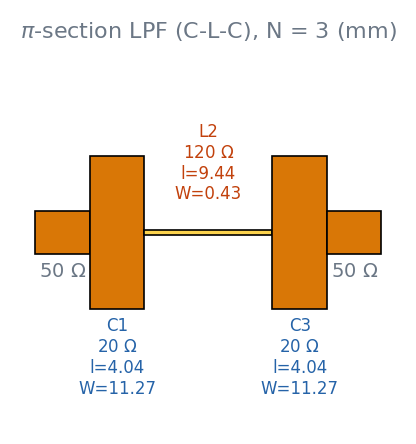
\includegraphics[width=\linewidth,height=3.3cm,keepaspectratio]{figs/c6_lay_pi3.png}
\begin{itemize}
  \item $g = 1, 2, 1$: pads $\beta l = 22.9^\circ$ (4.04 mm), line $47.7^\circ$ (9.44 mm).
\end{itemize}}{%
\lead{Double $\pi$-section, $N = 5$ (76 Bh)}
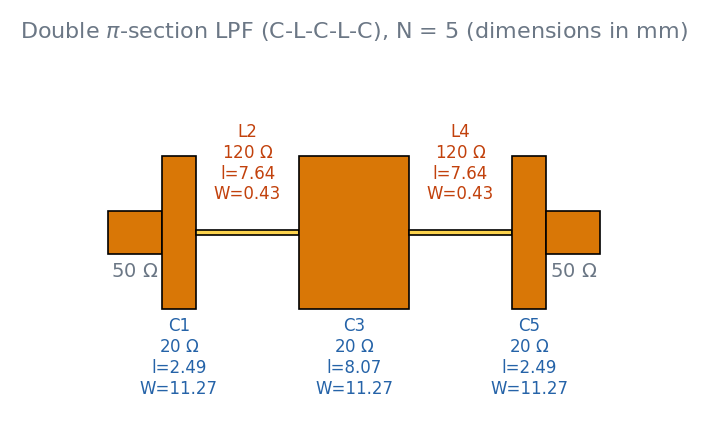
\includegraphics[width=\linewidth,height=3.3cm,keepaspectratio]{figs/c6_lay_pi5.png}
\begin{itemize}
  \item $g = 0.618, 1.618, 2, 1.618, 0.618$: three pads, two high-$Z$ lines.
\end{itemize}}

\par\penalty0\Needspace{14\baselineskip}
\sbs{%
\lead{Double-pad T-type, $N = 5$ (\texttt{81 Ba}; series-arm, 78 Ch)}
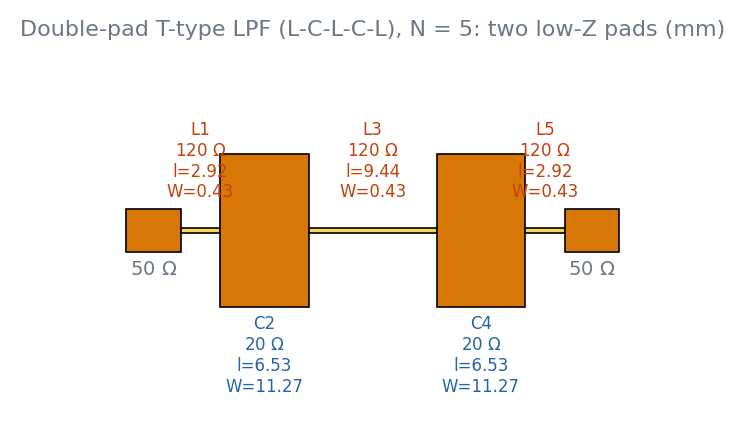
\includegraphics[width=\linewidth,height=3.3cm,keepaspectratio]{figs/c6_lay_t5.png}
\begin{itemize}
  \item L-C-L-C-L: the \textbf{series arms} are the three high-$Z$ lines, the two
    \textbf{pads} the shunt capacitors. A ``double-section series-arm'' filter is this
    layout.
\end{itemize}}{%
\lead{Double-section shunt-arm LPF, $N = 4$ (\texttt{80 Ba})}
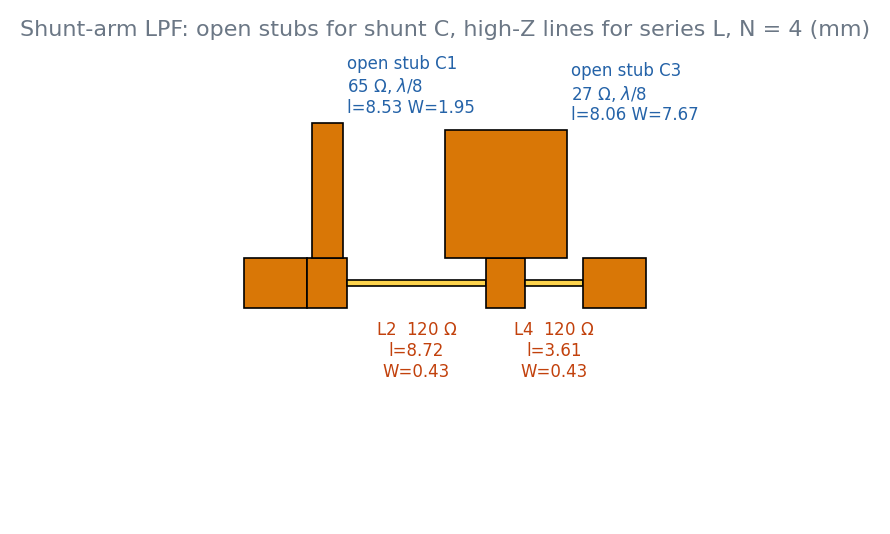
\includegraphics[width=\linewidth,height=3.3cm,keepaspectratio]{figs/c6_lay_stub.png}
\begin{itemize}
  \item Shunt capacitors as \textbf{open stubs}, $\lambda/8$ at $f_c$ with
    $Z = R_0/g_k$ (Richards): 65 and 27 $\Omega$; series inductors as high-$Z$ lines.
\end{itemize}}

\par\penalty0\Needspace{14\baselineskip}
\sbs{%
\lead{HPF $\pi$-section (74 Bh, \texttt{80 Bh}, \texttt{82 Ba})}
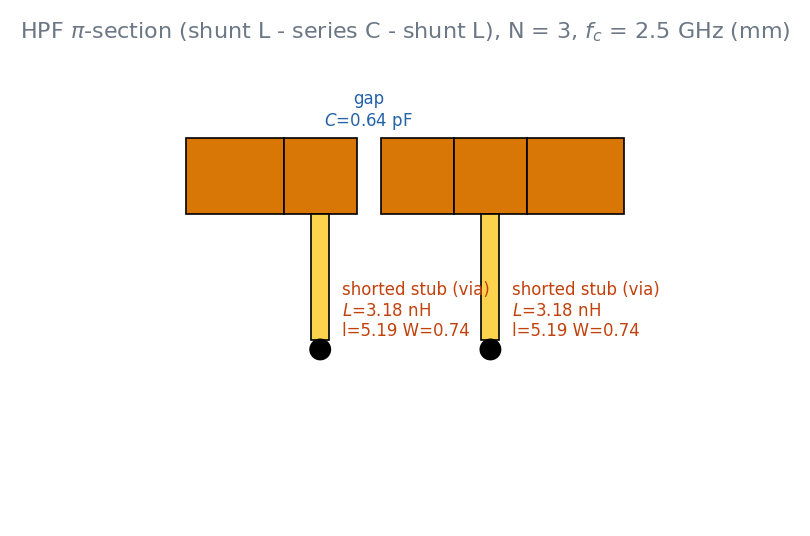
\includegraphics[width=\linewidth,height=3.3cm,keepaspectratio]{figs/c6_lay_hpf.png}
\begin{itemize}
  \item From the C-L-C prototype: shunt $L = 3.18$ nH, series $C = 0.637$ pF.
  \item Series capacitor = a \textbf{gap} (or interdigital) in the strip; shunt inductor =
    a \textbf{short-circuited stub} through a via: $Z_s\tan\beta l = \omega_cL$ gives
    5.19 mm of $100\,\Omega$ line.
  \item \textbf{Triple-pad series-arm HPF} (\texttt{82 Ba}): three pads separated by two
    gaps (the series capacitors) with shorted stubs from the pads.
  \item \texttt{80 Bh}'s ``second-order $\pi$'': one series gap between two stubbed pads.
\end{itemize}}{%
\lead{Single-section series-arm BPF (\texttt{81 Bh})}
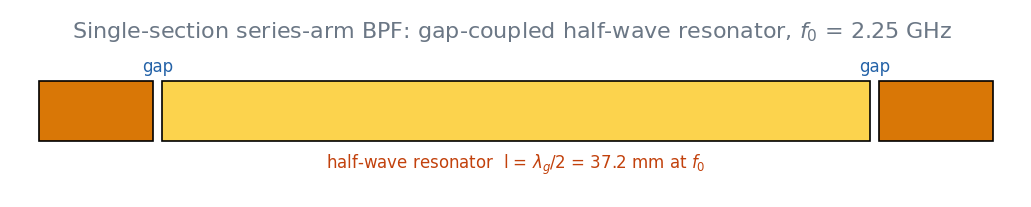
\includegraphics[width=\linewidth,height=3.3cm,keepaspectratio]{figs/c6_lay_bpf.png}
\begin{itemize}
  \item The series LC arm of a BPF is a \textbf{half-wave resonator} coupled by a gap at
    each end: resonant at $f_0$ (series-resonant, passes), capacitively coupled (blocks
    DC and low frequencies).
  \item $l = \lambda_g/2$ at $f_0$: 37.2 mm on 50 $\Omega$ at 2.25 GHz.
  \item More sections (more resonators) sharpen the skirts.
\end{itemize}}

\penalty0\vspace{2pt}

%=======================================================================
\T{6.4 RF Amplifier Theory: Gain, Stability and Design Flow}

\Q{Draw the design flowchart of a microwave amplifier; stability analysis; stability synthesis on the Smith chart; amplifier vs oscillator}{\m{4}\m{5}\m{3+8}\m{5+5}\m{6+4}\m{8}\m{10}}
{\color{sub}\footnotesize \tS{10} \yr{\textbf{71 Bh}, 71 Ma, \textbf{73 Bh}, \textbf{74 Bh}, \textbf{75 Bh}, \textbf{76 Bh}, \textbf{78 Ch}, \texttt{81 Ba}, \textbf{\texttt{81 Bh}}, \texttt{82 Ba}} \gap$\cdot$\gap the theory half of the amplifier questions}

\sbs{%
\lead{Reflection coefficients seen by the device}
\[ \Gamma_{in} = S_{11} + \frac{S_{12}S_{21}\Gamma_L}{1 - S_{22}\Gamma_L}
   = \frac{S_{11} - \Delta\Gamma_L}{1 - S_{22}\Gamma_L} \]
\[ \Gamma_{out} = S_{22} + \frac{S_{12}S_{21}\Gamma_S}{1 - S_{11}\Gamma_S}
   = \frac{S_{22} - \Delta\Gamma_S}{1 - S_{11}\Gamma_S} \]
{\color{sub}\footnotesize $\Delta = S_{11}S_{22} - S_{12}S_{21}$. From $b_2 = S_{21}a_1 + S_{22}\Gamma_Lb_2$ (deck slides 33 to 34).}
\lead{Three power gains}
\begin{itemize}
  \item \textbf{Transducer} $G_T = P_L/P_{avs}$ (the one the papers use).
  \item \textbf{Available} $G_A = P_{avn}/P_{avs}$; \textbf{operating}
    $G_P = P_L/P_{in}$.
\end{itemize}
\[ G_T = \frac{1 - |\Gamma_S|^2}{|1 - \Gamma_{in}\Gamma_S|^2}\,|S_{21}|^2\,
         \frac{1 - |\Gamma_L|^2}{|1 - S_{22}\Gamma_L|^2} \]
\begin{itemize}
  \item \textbf{Unilateral} ($S_{12} \approx 0$): $G_{TU} = G_S\,G_0\,G_L$ with
    $G_0 = |S_{21}|^2$; maximum at $\Gamma_S = S_{11}^*$, $\Gamma_L = S_{22}^*$:
    \[ G_{TU,max} = \frac{1}{1 - |S_{11}|^2}\,|S_{21}|^2\,\frac{1}{1 - |S_{22}|^2} \]
  \item \textbf{Unilateral figure of merit}
    $M = \dfrac{|S_{11}||S_{12}||S_{21}||S_{22}|}{(1 - |S_{11}|^2)(1 - |S_{22}|^2)}$;
    error bound $\dfrac{1}{(1 + M)^2} < \dfrac{G_T}{G_{TU}} < \dfrac{1}{(1 - M)^2}$.
    Unilateral is acceptable if the bound is a few tenths of a dB.
  \item \textbf{Bilateral maximum} (simultaneous conjugate match,
    $\Gamma_S = \Gamma_{in}^*$, $\Gamma_L = \Gamma_{out}^*$), only if unconditionally stable:
    \[ \Gamma_S = \frac{B_1 - \sqrt{B_1^2 - 4|C_1|^2}}{2C_1}, \quad
       \Gamma_L = \frac{B_2 - \sqrt{B_2^2 - 4|C_2|^2}}{2C_2} \]
    $B_1 = 1 + |S_{11}|^2 - |S_{22}|^2 - |\Delta|^2$, $C_1 = S_{11} - \Delta S_{22}^*$ (and
    $1 \leftrightarrow 2$). Then
    $G_{T,max} = \dfrac{|S_{21}|}{|S_{12}|}\left(K - \sqrt{K^2 - 1}\right)$.
\end{itemize}}{%
\lead{Stability}
\begin{itemize}
  \item \textbf{Oscillation} is possible if $|\Gamma_{in}| > 1$ or $|\Gamma_{out}| > 1$
    (negative resistance at a port).
  \item \textbf{Unconditionally stable}: $|\Gamma_{in}|, |\Gamma_{out}| < 1$ for
    \textbf{every} passive source and load. Test (Rollett):
    \[ K = \frac{1 - |S_{11}|^2 - |S_{22}|^2 + |\Delta|^2}{2|S_{12}S_{21}|} > 1
       \ \text{and}\ |\Delta| < 1 \]
    or the single test $\mu = \dfrac{1 - |S_{11}|^2}{|S_{22} - \Delta S_{11}^*| + |S_{12}S_{21}|} > 1$.
  \item \textbf{Conditionally (potentially) stable}: some $\Gamma_S$ or $\Gamma_L$ cause
    oscillation. Find them with \textbf{stability circles}:
    \[ C_L = \frac{(S_{22} - \Delta S_{11}^*)^*}{|S_{22}|^2 - |\Delta|^2}, \quad
       R_L = \left|\frac{S_{12}S_{21}}{|S_{22}|^2 - |\Delta|^2}\right| \]
    \[ C_S = \frac{(S_{11} - \Delta S_{22}^*)^*}{|S_{11}|^2 - |\Delta|^2}, \quad
       R_S = \left|\frac{S_{12}S_{21}}{|S_{11}|^2 - |\Delta|^2}\right| \]
  \item On the \textbf{output circle} $|\Gamma_{in}| = 1$; on the \textbf{input circle}
    $|\Gamma_{out}| = 1$. Each is a boundary, not a region.
\end{itemize}
\figT{c6_stab_circles.png}
{\color{sub}\scriptsize Deck slides 45 to 46: $S_{11} = 0.65\angle{-95^\circ}$ etc. at 800 MHz,
$K = 0.547$: $C_S = 1.79\angle122^\circ$, $R_S = 1.04$; $C_L = 1.30\angle48^\circ$,
$R_L = 0.45$. Hatched overlaps are the unstable $\Gamma$. Reproduced exactly in
\code{amp.py}.}}

\par\penalty0\Needspace{16\baselineskip}
\sbs{%
\lead{Which side of the circle is stable (synthesis on the Smith chart)}
\begin{enumerate}[label=\arabic*., leftmargin=1.4em, itemsep=1pt]
  \item Plot $C_L$, $R_L$ (and $C_S$, $R_S$) on the chart.
  \item Test the \textbf{centre} $\Gamma_L = 0$: there $|\Gamma_{in}| = |S_{11}|$.
  \item If $|S_{11}| < 1$ the centre is stable, so the stable region is the side of the
    circle that contains the centre:
  \begin{itemize}
    \item $|C_L| > R_L$ (centre outside) $\Rightarrow$ stable \textbf{outside} the circle.
    \item $|C_L| < R_L$ (centre inside) $\Rightarrow$ stable \textbf{inside}.
  \end{itemize}
  \item Same for the source circle with $|S_{22}|$.
  \item Circle entirely outside the unit chart (or enclosing it on the stable side)
    $\Rightarrow$ unconditionally stable. Circle cutting the chart $\Rightarrow$
    conditionally stable; choose $\Gamma_S$, $\Gamma_L$ well inside the stable part.
\end{enumerate}
{\color{sub}\footnotesize 73 Bh, 74 Bh, 75 Bh give a sketched chart; 71 Bh gives the circles
directly. Worked: companion Problem 7.}}{%
\lead{Amplifier design flowchart (write as boxes joined by arrows)}
\begin{enumerate}[label=\arabic*., leftmargin=1.4em, itemsep=1pt]
  \item \textbf{Specify} $f$, gain, noise figure, $Z_0$; \textbf{choose a transistor}
    (GaAs FET / HEMT / BJT) and bias; read its S-parameters.
  \item \textbf{Stability}: compute $\Delta$, $K$ (or $\mu$).
  \item $K > 1$, $|\Delta| < 1$? \textbf{Yes} $\rightarrow$ step 4. \textbf{No}
    $\rightarrow$ draw stability circles, restrict $\Gamma_S$, $\Gamma_L$ to the stable
    region (or add resistive loading / feedback), then step 4.
  \item \textbf{Unilateral check}: compute $M$ and the error bound.
  \begin{itemize}
    \item Small $\rightarrow$ $\Gamma_S = S_{11}^*$, $\Gamma_L = S_{22}^*$ (or gain
      circles for a specified gain).
    \item Large $\rightarrow$ bilateral: $\Gamma_S$, $\Gamma_L$ from $B$, $C$.
  \end{itemize}
  \item \textbf{Gain}: $G_{TU,max}$ or $G_{T,max}$; compare with the specification.
  \item \textbf{Matching networks}: realise $\Gamma_S$ and $\Gamma_L$ from $50\,\Omega$
    with a line plus a stub (Smith chart, Ch 2).
  \item \textbf{Bias network}, DC blocks, RF chokes; \textbf{layout} in microstrip;
    simulate, build, measure, tune.
\end{enumerate}
\figT{c6_amp_final.png}
{\color{sub}\scriptsize Final amplifier: input network, transistor, output network. Deck
slide 58.}}

\par\penalty0\Needspace{11\baselineskip}
\creamq{Amplifier circuit vs oscillator circuit in terms of stability factor}{\m{5}}
{\color{sub}\footnotesize \yr{71 Ma}}
\begin{tabularx}{\linewidth}{@{}L{2.6cm}XX@{}}
\toprule
\hrow & \thead{Amplifier} & \thead{Oscillator} \\
\midrule
Wanted & stable: no self-oscillation & unstable: oscillation on purpose \\
Stability factor & $K > 1$ and $|\Delta| < 1$ (or $\mu > 1$), or $\Gamma_S$, $\Gamma_L$ kept in the stable region & $K < 1$: device potentially unstable \\
Port reflection & $|\Gamma_{in}|, |\Gamma_{out}| < 1$ & $|\Gamma_{in}| > 1$ (negative resistance) \\
Terminations & conjugate match for gain & $\Gamma_S$ chosen \textbf{inside} the unstable region; $\Gamma_{in}\Gamma_S = 1$, $\Gamma_{out}\Gamma_L = 1$ \\
Input signal & required & none; starts from noise \\
Feedback & avoided, or negative & positive, loop gain $A\beta \ge 1$ \\
\bottomrule
\end{tabularx}

\par\penalty0\Needspace{8\baselineskip}
\Q{Stability and maximum gain numericals (bilateral and unilateral)}{\m{5+5}\m{10}\m{12}\m{15}\m{18}}
{\color{sub}\footnotesize \tS{22} \yr{\textbf{69 Bh}, \textbf{70 Bh}, 70 Ma, \textbf{71 Bh}, 71 Ma, \textbf{72 Ash}, 72 Ma, 73 Ma, \textbf{74 Bh}, 74 Ma, \textbf{76 Bh}, \textbf{77 Ch}, \textbf{78 Ch}, \textbf{\texttt{79 Bh}}, \textbf{79 Ch}, \texttt{80 Ba}, \textbf{\texttt{80 Bh}}, \textbf{80 Ch}, \texttt{81 Ba}, \textbf{\texttt{81 Bh}}, \texttt{82 Ba}, \textbf{\texttt{82 Bh}}} \gap$\cdot$\gap \mk{every set is solved in the companion}}
\begin{itemize}
  \item 13 distinct S-parameter sets across 22 papers; the companion works one in full,
    tabulates the rest with every intermediate, and splits out the cases that need a
    different answer (conditionally stable, given terminations, full matching design,
    circles given directly).
\end{itemize}

\penalty0\vspace{2pt}

%=======================================================================
\T{6.5 Microwave Oscillator Theory}

\Q{Microwave oscillator theory}{\m{8}}
{\color{sub}\footnotesize \tP{2} \yr{70 Ma, 71 Ma} \gap$\cdot$\gap 71 Ma as the amplifier-vs-oscillator contrast of $\S$6.4}

\sbsr{0.56}{%
\lead{Feedback view}
\begin{itemize}
  \item Gain $A$ with positive feedback $\beta$: $\dfrac{e_o}{e_i} = \dfrac{A}{1 - A\beta}$.
  \item $A\beta = 1$ $\rightarrow$ finite output with no input: \textbf{Barkhausen
    condition}. To start, $A\beta \approx 1.1$ to $1.2$; oscillation grows from noise until
    gain compression brings $A\beta$ back to 1.
\end{itemize}
\lead{Negative-resistance view (the microwave one)}
\begin{itemize}
  \item A device port with $|\Gamma_{out}| > 1$ has \textbf{negative resistance}.
  \item \textbf{One-port oscillator}: device $Z_{out} = R_{out} + jX_{out}$ with
    $R_{out} < 0$, load $Z_L$. Loop condition $\Gamma_{out}\Gamma_L = 1$ gives
    \[ R_L + R_{out} = 0, \qquad X_L + X_{out} = 0 \]
  \item To start oscillation the circuit must have net negative resistance:
    $R_L < |R_{out}|$. The deck's rule $|R_{out}| \ge 1.2R_L$ (Pozar uses
    $R_L = |R_{out}|/3$).
  \item \textbf{Two-port oscillator}: transistor with a \textbf{generator tuning network}
    ($\Gamma_S$) and a \textbf{load network} ($\Gamma_L$). Conditions:
    \begin{enumerate}[label=\arabic*., leftmargin=1.4em, itemsep=0pt]
      \item $K < 1$: device potentially unstable.
      \item $\Gamma_{in}\Gamma_S = 1$.
      \item $\Gamma_{out}\Gamma_L = 1$ (equivalent to 2, shown by substituting
        $\Gamma_{in}$).
    \end{enumerate}
\end{itemize}}{%
\figT{c6_feedback.png}
{\color{sub}\scriptsize Positive feedback. Deck slide 60.}
\vspace{2pt}

\figT{c6_twoport_osc.png}
{\color{sub}\scriptsize Two-port oscillator. Deck slide 62.}
\vspace{2pt}

\figT{c6_oneport.png}
{\color{sub}\scriptsize One-port: negative-resistance device and load. Deck slide 65.}}

\par\penalty0\Needspace{14\baselineskip}
\sbsr{0.62}{%
\lead{Two-port design steps}
\begin{enumerate}[label=\arabic*., leftmargin=1.4em, itemsep=1pt]
  \item From the S-parameters find $K$; need $K < 1$ (use a common-gate / common-base
    configuration or series feedback to make it so).
  \item Draw the \textbf{input stability circle}.
  \item Choose $\Gamma_S$ \textbf{inside the unstable region}, usually on the rim for the
    largest $|\Gamma_{out}|$; realise it with an inductor or shorted stub.
  \item $\Gamma_{out} = S_{22} + \dfrac{S_{12}S_{21}\Gamma_S}{1 - S_{11}\Gamma_S}$,
    $|\Gamma_{out}| > 1$ $\rightarrow$ $Z_{out} = R_{out} + jX_{out}$ with $R_{out} < 0$.
  \item Choose $R_L = |R_{out}|/3$ (start-up margin), $X_L = -X_{out}$; design the load
    matching network.
\end{enumerate}
\lead{Worked: Gunn diode one-port (deck slide 66, checked in \code{amp.py})}
\begin{itemize}
  \item $\Gamma_{out} = 1.24\angle30^\circ$ at 10 GHz. Plot $1/\Gamma_{out}^* = 0.806\angle30^\circ$,
    read $z$ and negate the real part: $Z_{out} = -68.9 + j159.0\,\Omega$ (deck reads
    $-70 + j160$).
  \item Resonance: $X_L = -159\,\Omega$, a capacitor $C = 1/(2\pi f\cdot159) = 0.100$ pF.
  \item Start-up: \textbf{the deck picks $R_L = 60\,\Omega$, which breaks its own rule}:
    $|R_{out}| \ge 1.2R_L$ needs $R_L \le 57.5\,\Omega$. Use $R_L = 23\,\Omega$ (Pozar's
    $|R_{out}|/3$) or at most $57\,\Omega$. \added{}
\end{itemize}}{%
\figT{c6_osc_steps.png}
{\color{sub}\scriptsize $\Gamma_S$ chosen inside the input stability circle. Deck slide 67.}
\lead{Oscillator types and stabilisation}
\begin{itemize}
  \item Transistor (FET, BJT), Gunn, IMPATT (one-port); YIG-tuned (wide tuning), DRO
    (dielectric resonator, low phase noise).
  \item Frequency stability: high-Q resonator in the tuning network; isolator at the
    output (Ch 4).
\end{itemize}}

\penalty0\vspace{2pt}

%=======================================================================
\T{6.6 Microwave Mixer}

\Q{Mixer theory / microwave mixer}{\m{5}}
{\color{sub}\footnotesize \tP{2} \yr{\textbf{70 Bh}, 72 Ma} \gap$\cdot$\gap \added{} the deck has no mixer slides; written from Pozar Ch 13}

\sbsr{0.56}{%
\begin{itemize}
  \item \textbf{Mixer}: a \textbf{nonlinear} three-port (diode or FET) that multiplies an
    RF signal $f_{RF}$ with a local oscillator $f_{LO}$ to translate it in frequency.
  \item Square-law principle: $i = a v^2$ with $v = V_{RF}\cos\omega_{RF}t + V_{LO}\cos\omega_{LO}t$
    contains $aV_{RF}V_{LO}\cos(\omega_{RF} \pm \omega_{LO})t$: \textbf{sum and difference}
    (checked by FFT in \code{amp.py}).
  \item \textbf{Down-conversion}: keep $f_{IF} = |f_{RF} - f_{LO}|$ with a filter; the
    \textbf{superheterodyne} receiver then amplifies at a fixed IF.
  \item \textbf{Up-conversion} (transmitters): keep $f_{RF} = f_{LO} + f_{IF}$.
  \item \textbf{Image frequency}: $f_{IM} = f_{LO} \pm f_{IF}$ on the other side of the LO
    also lands on $f_{IF}$ $\rightarrow$ reject it with an RF pre-filter or an
    image-reject mixer.
  \item \textbf{Figures of merit}: conversion loss $L_c = 10\log(P_{RF}/P_{IF})$
    (typically 4 to 7 dB for diode mixers), noise figure, LO-RF and LO-IF isolation,
    1 dB compression, intermodulation.
  \item \textbf{Types}:
  \begin{itemize}
    \item \textbf{Single-ended diode}: one Schottky diode; simple, poor isolation.
    \item \textbf{Balanced}: two diodes fed through a 90$^\circ$ or 180$^\circ$ hybrid
      (magic tee, rat race, Ch 4): cancels LO AM noise, better isolation, better input
      match.
    \item \textbf{Double-balanced}: diode ring with two baluns: suppresses even
      harmonics and both RF and LO at the IF port.
    \item \textbf{FET mixers}: conversion \textbf{gain} instead of loss.
  \end{itemize}
\end{itemize}}{%
\figT{c6_mixer_conv.png}
{\color{sub}\scriptsize (a) up-conversion, (b) down-conversion, each with its output
spectrum: both $f_{LO} \pm f_{IF}$ (or $f_{RF} \pm f_{LO}$) appear and a filter keeps one.
Pozar Fig 13.24.}
\vspace{3pt}
\figT{c6_mixer_diode.png}
{\color{sub}\scriptsize (a) single-ended diode mixer: RF and LO combined in a diplexing coupler,
DC-biased diode, low-pass filter to the IF port; (b) its ideal equivalent, $v_{RF} + v_{LO}$
across the diode. Pozar Fig 13.25.}}

\penalty0\vspace{2pt}

%=======================================================================
\T{6.7 PYQ Mapping}

\lead{Theory questions, covered in this document}
\begin{itemize}
  \item \textbf{Insertion loss method; why it is used} $\rightarrow$ $\S$6.1.
    \yr{\textbf{72 Ash} \m{5}, \textbf{73 Bh} \m{2+6}, 73 Ma \m{8}, \textbf{75 Bh} \m{5},
    \texttt{80 Ba} \m{3}, \textbf{\texttt{81 Bh}} \m{8}, \textbf{\texttt{82 Bh}} \m{3}}
  \item \textbf{Butterworth and Chebyshev common to prototype filters} $\rightarrow$ $\S$6.1.
    \yr{\textbf{70 Bh} \m{4}, 70 Ma \m{4}}
  \item \textbf{LPF prototyping (Butterworth, Chebyshev); filter parameters}
    $\rightarrow$ $\S$6.1. \yr{\textbf{72 Ash} \m{5}, 72 Ma \m{5}, 74 Ma \m{3}, \textbf{76 Bh} \m{8},
    \textbf{77 Ch} \m{8}, \textbf{\texttt{79 Bh}} \m{6}, \textbf{\texttt{80 Bh}} \m{10}}
  \item \textbf{Filter design steps; conversion to other filter types} $\rightarrow$ $\S$6.2.
    \yr{\textbf{71 Bh} \m{5}, \textbf{74 Bh} \m{6}, \textbf{\texttt{80 Bh}} \m{10}, \texttt{81 Ba} \m{7},
    \texttt{82 Ba} \m{7}, \textbf{\texttt{82 Bh}} \m{8}}
  \item \textbf{Microstrip implementation} (LPF $\pi$, double $\pi$, double-pad T, shunt-arm,
    series-arm, HPF, BPF) $\rightarrow$ $\S$6.3. \yr{\textbf{72 Ash} \m{3}, 73 Ma \m{2},
    \textbf{74 Bh} \m{4}, 74 Ma \m{5}, \textbf{76 Bh} \m{2}, \textbf{78 Ch} \m{10},
    \textbf{\texttt{79 Bh}} \m{2}, \texttt{80 Ba} \m{5}, \textbf{\texttt{80 Bh}} \m{10},
    \texttt{81 Ba} \m{3}, \textbf{\texttt{81 Bh}} \m{2}, \texttt{82 Ba} \m{3}, \textbf{\texttt{82 Bh}} \m{3}}
  \item \textbf{Design steps of a given 5th-order ladder (figure)} $\rightarrow$ companion
    Problem 10. \yr{\textbf{\texttt{82 Bh}} \m{3+8+3}}
  \item \textbf{Amplifier design flowchart} $\rightarrow$ $\S$6.4. \yr{\textbf{71 Bh} \m{5},
    \textbf{73 Bh} \m{10}, \textbf{74 Bh} \m{4}, \textbf{76 Bh} \m{4}, \textbf{78 Ch} \m{10},
    \texttt{81 Ba} \m{3}, \textbf{\texttt{81 Bh}} \m{3}, \texttt{82 Ba} \m{4}}
  \item \textbf{Stability analysis; synthesis from a sketched Smith chart} $\rightarrow$
    $\S$6.4 and companion Problem 7. \yr{\textbf{73 Bh} \m{10}, \textbf{74 Bh} \m{8},
    \textbf{75 Bh} \m{5}, \texttt{81 Ba} \m{4}, \texttt{82 Ba} \m{4}}
  \item \textbf{Stability of given circles $C_S, R_S, C_L, R_L$} $\rightarrow$ companion
    Problem 7. \yr{\textbf{71 Bh} \m{5}}
  \item \textbf{Amplifier vs oscillator in terms of stability factor} $\rightarrow$ $\S$6.4.
    \yr{71 Ma \m{5}}
  \item \textbf{Microwave oscillator theory} $\rightarrow$ $\S$6.5. \yr{70 Ma \m{8}}
  \item \textbf{Mixer theory} $\rightarrow$ $\S$6.6. \yr{\textbf{70 Bh} \m{5}, 72 Ma \m{5}}
\end{itemize}

\lead{Numerical content}
\begin{itemize}
  \item \textbf{This chapter has a numerical companion}, \textit{Ch6 - RF Design Practices -
    Numerical Problems and Solutions}: every amplifier S-parameter set in the archive
    (22 papers) and the 82 Bh filter design. All values from \code{src/amp.py} and
    \code{src/filt.py}.
\end{itemize}

\lead{Errors found and corrected}
\begin{itemize}
  \item Deck slide 51 (8 GHz example): $|\Delta| = 0.168$, $K = 3.53$; exactly
    $0.173$ and $3.445$ (verdict unchanged).
  \item Deck slide 52: $M = 0.04$ and bounds $-0.36$ to $+0.37$ dB; exactly $M = 0.034$,
    $-0.29$ to $+0.30$ dB.
  \item Deck slide 66: $R_L = 60\,\Omega$ violates the deck's own start-up rule.
  \item Deck example 8.6: $N = 5$ already meets 20 dB; $N = 6$ is conservative.
  \item Sorted PYQ documents: 71 Ma's set and marks, 70 Ma and 80 Ba asks, the missing
    75 Bh Smith-chart question and 72 Ma mixer note (fixed before this chapter).
\end{itemize}

\cleardoublepage
\section{Microwave Antennas and Propagation}
{\color{sub}\footnotesize 3 hrs \gap$\cdot$\gap asked in \mk{23 of 24 papers}
\gap$\cdot$\gap 3 syllabus sub-topics \gap$\cdot$\gap \mk{162 marks, 7.8\% of the archive} \gap$\cdot$\gap \mk{30 numerical (19\%) + 132 theory}
$\rightarrow$ almost every mark is on sub-topic (c), radiation hazards; antenna types and
propagation have never been examined.}

\vspace{3pt}\noindent
\colorbox{gdL}{\makebox[\dimexpr\textwidth-2\fboxsep][l]{%
  \textcolor{gd}{\bfseries\footnotesize READ THIS FIRST}}}
\par\nobreak\vspace{3pt}

Chapter 7 is the \mk{one guaranteed question} of the paper: only 72 Ash skips it in 24 sets.
It comes as a 4 to 10 mark theory answer, usually two parts glued together.
\begin{enumerate}[label=\arabic*., leftmargin=1.4em, itemsep=1pt]
  \item \textbf{Radiation fields / zones} (11 papers) $\rightarrow$ $\S$7.1. Three zones, two
    boundary formulas, one figure. The BTS and microwave-oven versions put numbers in them:
    worked in the \textbf{numerical companion}.
  \item \textbf{How microwaves are hazardous; HERP, HERO, HERF} (17 papers) $\rightarrow$
    $\S$7.2. Always the same chain: non-ionizing $\rightarrow$ dielectric heating
    $\rightarrow$ no internal heat sensors $\rightarrow$ poorly cooled organs.
  \item \textbf{SAR} (3 papers, one of them for 10 marks) $\rightarrow$ $\S$7.3.
  \item \textbf{Safety standards} (4 papers) and \textbf{safety practices} (7 papers)
    $\rightarrow$ $\S$7.4 and $\S$7.5. Name the body, the frequency range and one number each.
\end{enumerate}
Two things worth knowing before the paper starts:
\begin{itemize}
  \item Nearly every question is ``part A + part B'' from the list above. Answer each part
    under its own heading and draw the zone figure whenever ``fields'' appears.
  \item \textbf{Every limit is built on one number}: a whole-body SAR of \mk{4 W/kg} warms
    the body by about 1$^\circ$C. Divide by 10 for workers (0.4 W/kg), by 50 for the public
    (0.08 W/kg). Quote this and the standards section writes itself.
\end{itemize}

\hr

%=======================================================================
\T{7.1 Microwave Radiation Fields (Radiation Zones)}

\Q{Name and explain the microwave radiation fields: reactive, radiating near and far field}{\m{5}\m{4}\m{3}\m{8}\m{5+5}}
{\color{sub}\footnotesize \tS{11} \yr{\textbf{69 Bh}, 71 Ma, 72 Ma, 74 Ma, \textbf{76 Bh}, \textbf{77 Ch}, \textbf{79 Ch}, \texttt{80 Ba}, \texttt{81 Ba}, \textbf{\texttt{81 Bh}}, \texttt{82 Ba}} \gap$\cdot$\gap oven (74 Ma, 77 Ch) and BTS (81 Ba, 81 Bh, 82 Ba) versions}

\sbsr{0.50}{%
\begin{itemize}
  \item \textbf{Radiation} = energy carried away by EM waves. Round any antenna (or leaking
    oven, or waveguide opening) the field is split into \textbf{three zones} by distance $R$,
    antenna largest dimension $D$ and wavelength $\lambda$.
  \item \textbf{Near field} = the first two zones. \textbf{Far field} = the third.
\end{itemize}
\vspace{2pt}
\begin{tabularx}{\linewidth}{@{}L{2.0cm}X@{}}
\toprule
\hrow \thead{Zone} & \thead{Boundary} \\
\midrule
Reactive near field & $R < 0.62\sqrt{D^3/\lambda}$ \\
Radiating near field (Fresnel) & $0.62\sqrt{D^3/\lambda} < R < 2D^2/\lambda$ \\
Far field (Fraunhofer) & $R > 2D^2/\lambda$ \\
\bottomrule
\end{tabularx}}{%
\figT{c7_zones.png}
{\color{sub}\scriptsize Reactive and radiating near field, then far field. Karkee, Ch-7 PDF
p5 (white on black in the source, inverted for print).}}

\par\penalty0\Needspace{14\baselineskip}
\lead{What each zone is like (the ``differentiate'' answer, 79 Ch, 72 Ma)}
\begin{tabularx}{\linewidth}{@{}L{2.4cm}XXX@{}}
\toprule
\hrow & \thead{Reactive near field} & \thead{Radiating near field} & \thead{Far field} \\
\midrule
Energy & \textbf{stored}, sloshes back and forth to the antenna each cycle & radiated, but beam still forming & radiated, travelling away \\
$E$ and $H$ & $90^\circ$ out of phase, not in fixed ratio & in phase, ratio settling & in phase, $E \perp H \perp$ direction \\
$E/H$ & not 377 $\Omega$; measure $E$ and $H$ separately & approaching 377 $\Omega$ & $= 377\,\Omega$, so $S = E^2/377$ \\
Fall with $R$ & fast ($1/R^2$ to $1/R^3$) & irregular, local peaks & $S \propto 1/R^2$ \\
Pattern & not defined & changes with distance & fixed shape \\
Hazard & \textbf{highest}: body close enough couples to stored energy & high: full beam power in a column about $D$ wide & lowest, and predictable from $S = P_tG/4\pi R^2$ \\
\bottomrule
\end{tabularx}

\par\penalty0\Needspace{10\baselineskip}
\begin{itemize}
  \item \textbf{Hazardous vs safe} (deck): reactive and radiating near field are treated as
    \textbf{hazardous}, the far field as the \textbf{safe} side, where exposure falls as
    $1/R^2$ and can be checked against a limit ($\S$7.4).
  \item \textbf{Validity} \added{}: the two formulas assume an antenna \textbf{larger than a
    wavelength}. For a small antenna ($D < \lambda$, e.g. a quarter-wave whip) they give a
    ``far field'' that starts inside the reactive region. Use instead: reactive field out to
    $\lambda/2\pi$, far field beyond about $2\lambda$. The 82 Ba quarter-wave question and the
    deck's 150 MHz example fall here (\code{ant.py}).
\end{itemize}

\par\penalty0\Needspace{12\baselineskip}
\creamq{Radiation zones of a microwave oven; radiation fields round a GSM BTS}{\m{3}\m{4}\m{4}\m{4}}
{\color{sub}\footnotesize \yr{74 Ma, \textbf{77 Ch} (oven); \texttt{81 Ba}, \textbf{\texttt{81 Bh}}, \texttt{82 Ba} (BTS)} \gap$\cdot$\gap full working in the numerical companion}
\sbs{%
\lead{Microwave oven, $f = 2.45$ GHz, $D = 0.5$ m}
\begin{itemize}
  \item $\lambda = 0.1224$ m, $D > \lambda$ so the formulas hold.
  \item Reactive: $R < 0.63$ m. Fresnel: $0.63$ to $4.08$ m. Far field: $R > 4.08$ m.
  \item \textbf{In practice} the cavity is a closed metal box (Faraday cage) and the door mesh
    holes are far smaller than $\lambda = 12$ cm, so almost nothing leaks. Leakage limit (US
    FDA): \mk{1 mW/cm$^2$ at 5 cm} when sold, 5 mW/cm$^2$ over its life. \added{}
  \item Zones matter only for leakage at a damaged door seal or hinge: stay out of the
    reactive zone (arm's length) while it runs.
\end{itemize}}{%
\lead{GSM / LTE base station (BTS)}
\begin{itemize}
  \item Panel antenna on a mast, main beam tilted a few degrees down, hitting the ground
    tens to hundreds of metres away (figure).
  \item \textbf{Reactive and Fresnel zones}: within a few metres \textbf{in front of} the
    panel, reached only by riggers on the tower or a rooftop $\rightarrow$
    \textbf{occupational} exclusion zone.
  \item \textbf{Far field}: everywhere the public is. Power density there is far below the
    limit (81 Bh: zones $0.65$ m and $4.33$ m).
  \item \textbf{Radiation parameters} (81 Ba): frequency, transmit power, antenna gain,
    EIRP, beam tilt and beamwidth, polarization, power density (W/m$^2$), field strength
    (V/m), SAR.
\end{itemize}
\figT{c7_tower.png}
{\color{sub}\scriptsize Main beam of a mast-mounted antenna. KEC Ch-7 deck, slide 32.}}

\penalty0\vspace{2pt}

%=======================================================================
\T{7.2 How Microwave Radiation Is Hazardous: HERP, HERO, HERF}

\Q{How are microwaves hazardous to humans (living body)? Microwave radiation hazards (short note)}{\m{3}\m{4}\m{5}\m{6}\m{8}}
{\color{sub}\footnotesize \tS{17} \yr{\textbf{69 Bh}, \textbf{70 Bh}, 70 Ma, \textbf{71 Bh}, 72 Ma, 73 Ma, \textbf{73 Bh}, 74 Ma, \textbf{74 Bh}, \textbf{75 Bh}, \textbf{77 Ch}, \textbf{78 Ch}, \textbf{\texttt{79 Bh}}, \textbf{\texttt{80 Bh}}, \textbf{\texttt{81 Bh}}, \texttt{82 Ba}, \textbf{\texttt{82 Bh}}} \gap$\cdot$\gap \mk{the most repeated ask of the chapter}}

\sbsr{0.60}{%
\lead{1. Microwaves are non-ionizing}
\begin{itemize}
  \item Photon energy $E = hf$: at 2.45 GHz only $1.0\times10^{-5}$ eV.
  \item Ionizing a molecule needs about 10 eV $\rightarrow$ a microwave photon is a
    \textbf{million times} too weak. It cannot break bonds or DNA directly (unlike
    X-rays, gamma rays).
  \item So the established hazard is \textbf{heat}, not ionization.
\end{itemize}
\lead{2. Thermal effect: dielectric heating}
\begin{itemize}
  \item The field \textbf{rotates polar water molecules} and drives \textbf{ionic currents}
    in tissue $\rightarrow$ friction and $I^2R$ loss $\rightarrow$ heat.
  \item Absorbed power per kg $= \sigma E^2/\rho$ = \textbf{SAR} ($\S$7.3).
  \item Microwaves heat \textbf{inside out}. Sunlight heats \textbf{outside in}, where skin
    sensors warn and sweat cools (figure).
\end{itemize}}{%
\figT{c7_heating.png}
{\color{sub}\scriptsize Sun heating (outside in, felt) vs microwave heating (inside out,
trapped). Gangaju, Ch-7 deck, slide 4.}
\vspace{3pt}

\figT{c7_spectrum.png}
{\color{sub}\scriptsize Microwaves sit far below visible light and the ionizing bands. KEC
Ch-7 deck, slide 5.}}

\par\penalty0\Needspace{14\baselineskip}
\lead{3. Why the heating is dangerous}
\begin{itemize}
  \item \textbf{No internal heat sensation}: the body senses heat only in the skin, so deep
    tissue can be damaged \textbf{before the person notices}.
  \item \textbf{Poorly cooled organs} (little blood flow to carry heat away):
  \begin{itemize}
    \item \textbf{Eye lens} $\rightarrow$ cataract.
    \item \textbf{Testes} $\rightarrow$ temporary sterility.
    \item Stomach, intestines, bladder, gall bladder $\rightarrow$ thermal damage at high power.
  \end{itemize}
  \item \textbf{Body resonance}: absorption peaks when body size is comparable to $\lambda$
    (whole adult body about 70 to 100 MHz). The deck adds: significant absorption even when
    body size is $\lambda/10$. That is why every limit chart dips lowest at 30 to 300 MHz
    ($\S$7.4).
  \item \textbf{Penetration falls with frequency}: deep at UHF (several cm), about 1 to 2 cm
    at 2.45 GHz, only the skin above about 10 GHz $\rightarrow$ lower microwave bands heat
    deep tissue unfelt, higher bands burn the surface. \added{}
  \item Long low-frequency magnetic exposure can also induce damaging currents (deck).
\end{itemize}

\par\penalty0\Needspace{12\baselineskip}
\lead{4. Other effects}
\begin{itemize}
  \item \textbf{RF burns and shocks}: touching a metal object (fence, mast, vehicle) in a
    strong field drives \textbf{contact current} through the hand.
  \item \textbf{Implants}: pacemakers and other active implants can malfunction; metal
    implants concentrate the field and heat.
  \item \textbf{Microwave hearing}: pulsed radar is heard as clicks (thermoelastic
    expansion in the head).
  \item \textbf{Behavioural complaints} reported by RF workers: headache, irritability,
    fatigue, sleeplessness (deck). Not reproduced in blind studies.
  \item \textbf{Cancer}: IARC (WHO) 2011 classes RF fields \textbf{Group 2B, ``possibly
    carcinogenic''}, meaning limited evidence. \mk{Correction}: one student deck calls
    microwaves ``known'' to cause cancer and another slide calls non-thermal effects
    ``several times more harmful'' than thermal; neither is established. \added{}
\end{itemize}

\par\penalty0\Needspace{12\baselineskip}
\creamq{Link to the zones (69 Bh, 72 Ma, 81 Bh): ``how is non-radiating radiation hazardous?''}{\m{4}\m{5}\m{8}}
\begin{itemize}
  \item The \textbf{reactive near field} does not radiate, but its stored $E$ and $H$ fields
    are strongest there. A body inside it \textbf{loads} the antenna and \textbf{draws energy
    out} of the stored field $\rightarrow$ absorbed as heat, although nothing is ``radiated''.
  \item Radiating near field: full beam power confined to a column about the antenna's size
    $\rightarrow$ highest power density a person in front of the antenna meets.
  \item Far field: $S = P_tG/4\pi R^2$ falls with distance $\rightarrow$ distance is the
    simplest protection ($\S$7.5).
\end{itemize}

\par\penalty0\Needspace{14\baselineskip}
\creamq{Types of electromagnetic radiation hazard (RADHAZ); HERP short note}{\m{4}}
{\color{sub}\footnotesize \yr{74 Ma (types), \textbf{\texttt{80 Bh}} (HERP)}}
\par\noindent
\begin{minipage}[t]{0.31\textwidth}\vspace{0pt}\raggedright
\lead{HERP: to personnel}
\begin{itemize}
  \item Harmful \textbf{biological} effects in humans.
  \item Cause: thermal effect of absorbed energy (points 2 and 3 above).
  \item Eg: eye lens exposed $\rightarrow$ too little blood flow to cool it $\rightarrow$
    cataract.
  \item Controlled by exposure limits (SAR, power density).
  \item \textcolor{sub}{\small ``Hazards of Electromagnetic Radiation to Personnel''.}
\end{itemize}\end{minipage}\hfill
\begin{minipage}[t]{0.33\textwidth}\vspace{0pt}\raggedright
\lead{HERO: to ordnance}
\begin{itemize}
  \item RF induces current in the leads of \textbf{electro-explosive devices} (EEDs: detonators,
    squibs, airbag igniters, missile motors) $\rightarrow$ \textbf{premature firing}.
  \item Ordnance is \textbf{more sensitive} than people: no blood flow to shed heat.
  \item But easier to protect: metal enclosures reflect the field.
  \item A chain explosion is possible $\rightarrow$ HERO limits are \textbf{lower} than
    personnel limits.
\end{itemize}\end{minipage}\hfill
\begin{minipage}[t]{0.33\textwidth}\vspace{0pt}\raggedright
\lead{HERF: to fuel}
\begin{itemize}
  \item RF-induced \textbf{arcs} ignite \textbf{fuel vapour} during refuelling near radar or
    radio transmitters.
  \item Ignition likely for arcs above about \textbf{50 VA}.
  \item Rules (deck):
  \begin{itemize}
    \item no transmitting from a vehicle or aircraft being fuelled, or the one beside it
    \item no connecting or breaking cables or ground wires while fuelling
    \item radar lighting the area at 5 W/cm$^2$ peak: shut off
    \item antennas of 250 W or less at least 50 ft from fuelling (500 W at sea)
  \end{itemize}
\end{itemize}\end{minipage}\par

\penalty0\vspace{2pt}

%=======================================================================
\T{7.3 Specific Absorption Rate (SAR)}

\Q{Define SAR. Discuss microwave radiation hazards based on SAR exposures; what is non-ionizing SAR}{\m{4}\m{6}\m{10}}
{\color{sub}\footnotesize \tF{3} \yr{\textbf{74 Bh}, \textbf{80 Ch}, \texttt{81 Ba}} \gap$\cdot$\gap 80 Ch sets the whole 10 marks on it}

\lead{Definition}
\begin{itemize}
  \item \textbf{SAR} = rate at which RF energy is \textbf{absorbed per unit mass} of body
    tissue, in \textbf{W/kg}.
    \[ \boxed{\mathrm{SAR} = \frac{d}{dt}\left(\frac{dW}{dm}\right) = \frac{\sigma E^2}{\rho} = c\,\frac{dT}{dt}} \]
  \item $\sigma$ = tissue conductivity (S/m), $E$ = \textbf{rms field inside the tissue}
    (V/m), $\rho$ = mass density (\textbf{kg/m$^3$}), $c$ = specific heat (J/kg K),
    $dT/dt$ = initial temperature rise rate.
\end{itemize}

\sbsr{0.52}{%
\begin{itemize}
  \item \mk{Correction}: the deck prints the density unit as kg/m$^2$; a mass density is
    kg/m$^3$, which is what makes $\sigma E^2/\rho$ come out in W/kg. \added{}
  \item \textbf{Non-ionizing SAR} (81 Ba): SAR measures \textbf{heating} from non-ionizing
    RF. It is the dose quantity for RF the way absorbed dose (Gy) is for ionizing radiation.
\end{itemize}}{%
\lead{Averaging and measurement}
\begin{itemize}
  \item \textbf{Whole-body SAR}: total absorbed power / body mass.
  \item \textbf{Localized (peak spatial) SAR}: averaged over any \textbf{1 g} (FCC) or
    \textbf{10 g} (ICNIRP, IEEE 2019) cube of tissue: the phone-against-head case.
  \item Averaged over time (6 min in ICNIRP 1998).
  \item \textbf{Measured} with a phantom head or body filled with tissue-simulating liquid: a
    robot moves an $E$-field probe through it (SAR $= \sigma E^2/\rho$), or a temperature probe
    logs $dT/dt$ (SAR $= c\,dT/dt$).
  \item Eg (\code{ant.py}): muscle at 900 MHz, $\sigma \approx 0.94$ S/m,
    $\rho \approx 1040$ kg/m$^3$; $E = 10$ V/m inside gives $0.09$ W/kg.
\end{itemize}}

\par\penalty0\Needspace{16\baselineskip}
\lead{Hazards based on SAR exposure (the 10-mark body)}
\begin{tabularx}{\linewidth}{@{}L{3.3cm}X@{}}
\toprule
\hrow \thead{Whole-body SAR} & \thead{Effect and what the standards do with it} \\
\midrule
below 0.08 W/kg & \textbf{public limit}. No established health effect. \\
0.4 W/kg & \textbf{occupational limit} for trained workers. \\
about 1 to 4 W/kg & body temperature rises up to about $1^\circ$C, thermoregulation (blood flow, sweat) copes in healthy adults. \\
\textbf{4 W/kg} & \textbf{threshold}: about $1^\circ$C core rise, animals show disrupted behaviour. With no heat loss, 4 W/kg warms tissue 1$^\circ$C in about 15 min ($c \approx 3500$ J/kg K). \\
well above 4 W/kg & heat stress, heat stroke; local hot spots burn tissue, cataract in poorly cooled lens. \\
\bottomrule
\end{tabularx}
\par\penalty0\Needspace{8\baselineskip}
\begin{itemize}
  \item \textbf{Safety factors}: threshold $4 \xrightarrow{\div 10} 0.4$ (occupational)
    $\xrightarrow{\div 5} 0.08$ W/kg (public). The student deck's ``one-tenth of the observed
    threshold SAR (0.4 W/kg)'' means the \textbf{limit} is 0.4; the threshold is 4. \added{}
  \item \textbf{Localized SAR limits}: public 2 W/kg over 10 g head and trunk (ICNIRP, IEEE
    2019), \textbf{1.6 W/kg over 1 g} (FCC, US and India phones); workers 10 W/kg.
  \item \textbf{Mobile phones}: SAR is declared by the maker (typically 0.2 to 1.6 W/kg).
    Using a hands-free kit or speaker cuts it sharply because the head leaves the reactive
    near field of the handset antenna.
\end{itemize}

\penalty0\vspace{2pt}

%=======================================================================
\T{7.4 International EMR Safety Standards}

\Q{International standards and recommended practices (SARPs) for RF/microwave exposure; IEEE safety standard}{\m{2}\m{3}\m{3+3}\m{5+5}}
{\color{sub}\footnotesize \tF{4} \yr{70 Ma, \textbf{76 Bh}, \texttt{80 Ba}, \texttt{82 Ba}} \gap$\cdot$\gap practices half in $\S$7.5}

\begin{itemize}
  \item \textbf{Basis of all of them}: adverse effects scale with absorbed power $\rightarrow$
    \textbf{basic restriction} in SAR (W/kg), and because SAR cannot be measured in a person,
    a \textbf{reference level} (MPE) in measurable power density (mW/cm$^2$, W/m$^2$) or
    field strength (V/m, A/m).
  \item \textbf{Two tiers}: \textbf{occupational / controlled} (trained workers who know they
    are exposed) and \textbf{general public / uncontrolled} (everyone else, 24 hours a day,
    including children, the ill and the elderly) $\rightarrow$ public limit 5 times lower.
  \item $1 \text{ mW/cm}^2 = 10 \text{ W/m}^2$.
\end{itemize}

\par\penalty0\Needspace{20\baselineskip}
\begin{tabularx}{\linewidth}{@{}L{2.9cm}L{2.2cm}X@{}}
\toprule
\hrow \thead{Body and standard} & \thead{Range} & \thead{Key numbers} \\
\midrule
\textbf{IEEE / ANSI C95.1} (US; 1982, 2005, 2019) & 3 kHz to 300 GHz (0 Hz to 300 GHz in 2019) & 1982 single tier: 1 mW/cm$^2$ at 30 to 300 MHz, $f/300$ to 1.5 GHz, 5 mW/cm$^2$ above. 2005/2019: two tiers, whole body 0.08 / 0.4 W/kg, local 2 / 10 W/kg over 10 g (2019). \\
\textbf{FCC} (US, OET Bulletin 65) & 300 kHz to 100 GHz & public 0.2 mW/cm$^2$ at 30 to 300 MHz, $f/1500$ to 1.5 GHz, 1.0 mW/cm$^2$ above; occupational 5 times higher. Phone SAR 1.6 W/kg over 1 g. Averaging 6 min (workers), 30 min (public). \\
\textbf{ICNIRP} (international, recognized by WHO; 1998, revised 2020) & 100 kHz to 300 GHz & public $f/200$ W/m$^2$ at 400 to 2000 MHz (4.5 at 900, 9 at 1800), 10 W/m$^2$ above 2 GHz; workers 5 times. SAR 0.08 / 0.4 W/kg whole body, 2 / 10 W/kg local. Adopted by most countries. \\
\textbf{IRPA / INIRC} (1988) & & ICNIRP's predecessor: first international occupational and public limits. \\
\textbf{OSHA} (US workplaces) & 10 MHz to 100 GHz & 10 mW/cm$^2$ averaged over 6 min (older guide). \\
\textbf{ITU-T K.52, K.70} & telecom sites & how to check a BTS site against ICNIRP limits, and how to mitigate (compliance distance, exclusion zones). \\
\textbf{WHO EMF Project, IARC} & & reviews health evidence; IARC Group 2B (2011). \\
\bottomrule
\end{tabularx}

\par\penalty0\Needspace{16\baselineskip}
\sbs{%
\figT{c7_fcc.png}
{\color{sub}\scriptsize \textbf{FCC MPE} (power density, mW/cm$^2$, vs MHz): solid occupational,
dashed public. Karkee PDF p18.}}{%
\figT{c7_ansi.png}
{\color{sub}\scriptsize \textbf{ANSI C95.1-1982} Radiation Protection Guide. Karkee PDF p19.}}

\par\penalty0\Needspace{8\baselineskip}
\begin{itemize}
  \item \textbf{Read the charts}: both dip at \textbf{30 to 300 MHz}, the body-resonance band
    ($\S$7.2), and rise again above 300 MHz as absorption becomes shallower.
  \item \mk{Correction}: the deck's ``IRPA permissible exposure level'' table (PDF p17: 200
    $\mu$T, 5 kV/m, 20 mV/m in the head) is ICNIRP's \textbf{50 Hz power-line} limit, not a
    microwave one. It is left out here. \added{}
  \item \textbf{SARPs} (80 Ba) = \textbf{Standards And Recommended Practices}: answer with the
    ICNIRP / IEEE limits above as the standards and $\S$7.5 as the practices.
\end{itemize}

\penalty0\vspace{2pt}

%=======================================================================
\T{7.5 RF/Microwave Safety Practices}

\Q{RF/MW radiation hazards and safety practices; list and describe five major RF safety practices}{\m{3}\m{5}\m{6}\m{5+5}}
{\color{sub}\footnotesize \tS{7} \yr{\textbf{70 Bh}, \textbf{71 Bh}, \textbf{73 Bh}, \textbf{74 Bh}, \textbf{76 Bh}, \textbf{79 Ch}, \textbf{\texttt{79 Bh}}} \gap$\cdot$\gap short-note form mostly; hazard half is $\S$7.2}

\sbsr{0.68}{%
\lead{Five major practices (79 Ch)}
\begin{enumerate}[label=\arabic*., leftmargin=1.4em, itemsep=1pt]
  \item \textbf{Time, distance, shielding}:
  \begin{itemize}
    \item cut exposure time
    \item keep out of the main beam and out of the near field (power density $\propto 1/R^2$)
    \item metal panels or mesh, RF absorbers, Faraday enclosures
  \end{itemize}
  \item \textbf{Engineering controls}:
  \begin{itemize}
    \item safety \textbf{interlocks} that cut RF when a door or panel opens
    \item RF gaskets, choke joints, oven door mesh
    \item test into a \textbf{dummy load}, never an open waveguide
    \item grounding straps not bent at sharp angles (they radiate)
  \end{itemize}
  \item \textbf{Administrative controls}:
  \begin{itemize}
    \item RF survey of the site, marked \textbf{exclusion zones}, warning signs (figure)
    \item \textbf{lockout / tagout} before work on a tower or transmitter
    \item never look into a live waveguide, horn or dish
    \item training and exposure records
  \end{itemize}
  \item \textbf{Personal protective equipment}: RF protective suit (stainless steel woven into
    fire-retardant fibre) for high-field areas; personal RF monitor that alarms.
  \item \textbf{Regular inspection}:
  \begin{itemize}
    \item \textbf{visual}: housekeeping, interlocks present, high-voltage grounding rods,
      condition of cables and coax, RF shielding intact
    \item \textbf{operational}: RF level survey in occupied spaces, interlock tests, lockout
      used properly
  \end{itemize}
\end{enumerate}}{%
\figT{c7_warning.png}
{\color{sub}\scriptsize RF warning sign at an exclusion-zone boundary. KEC Ch-7 deck, slide 24.}
\vspace{4pt}

\lead{More practices (deck)}
\begin{itemize}
  \item Operate stray-RF sources (induction and dielectric heaters) \textbf{remotely}.
  \item Keep workers below the recommended limits ($\S$7.4).
  \item \textbf{HERO}: keep EEDs away from transmitters.
  \item \textbf{HERF}: no RF devices in flammable atmospheres; fuelling rules of $\S$7.2.
  \item RF-sensitive equipment and people with \textbf{implants} away from sources.
  \item Switch equipment off when not in use.
  \item \textbf{Public}: antennas high and beams tilted clear of rooftops; hands-free phones;
    awareness and school teaching.
\end{itemize}}

\penalty0\vspace{2pt}

%=======================================================================
\T{7.6 Microwave Antennas}

\Q{Microwave antenna types}{\pill{gdL}{gd}{syllabus, no PYQ yet}}
{\color{sub}\footnotesize syllabus 7(a) \gap$\cdot$\gap the deck leaves it as an assignment and refers to Pozar}

\begin{itemize}
  \item Conventional wire antennas work at microwaves too, but the short wavelength allows
    \textbf{aperture antennas} a few $\lambda$ across $\rightarrow$ high gain, narrow beams in a
    small size.
  \item \textbf{Parameters}: gain $G$ and directivity, beamwidth, efficiency, polarization,
    input impedance / VSWR, bandwidth. Aperture gain
    $G = 4\pi A_e/\lambda^2$ with $A_e = \eta\,\pi D^2/4$.
\end{itemize}

\par\penalty0\Needspace{16\baselineskip}
\sbsr{0.72}{%
\begin{tabularx}{\linewidth}{@{}L{1.9cm}XL{2.3cm}@{}}
\toprule
\hrow \thead{Type} & \thead{How it works} & \thead{Typical use} \\
\midrule
\textbf{Horn} & flared end of a waveguide; flare matches guide to free space. E-plane, H-plane, pyramidal, conical. 10 to 25 dBi & dish feed, gain standard in measurements \\
\textbf{Parabolic reflector} & feed (horn) at focus; reflector turns spherical wave into plane wave. $G = \eta(\pi D/\lambda)^2$, HPBW $\approx 70\lambda/D$ degrees. Front-fed or Cassegrain & satellite earth stations, radar, point-to-point links \\
\textbf{Lens} & dielectric (slows wave) or metal-plate (speeds it) lens collimates like an optical lens & mm-wave radar, automotive \\
\textbf{Slot} & slot cut in a waveguide wall or ground plane; complement of a dipole (Babinet); flush & aircraft, slotted-guide arrays \\
\textbf{Microstrip patch} & metal patch about $\lambda_g/2$ long over a ground plane on a substrate; low profile, narrow band (1 to 5\%), low power; arrays & phones, GPS, WLAN, 5G arrays \\
\textbf{Helical} & wire helix; axial mode when circumference $\approx \lambda$ $\rightarrow$ circular polarization & satellite, space telemetry \\
\bottomrule
\end{tabularx}
{\color{sub}\footnotesize Eg (\code{ant.py}): 1.2 m dish at 12 GHz, $\eta = 0.55$: $G = 41.0$ dBi, HPBW $= 1.46^\circ$.}}{%
\figT{c7_horn.png}
{\color{sub}\scriptsize Pyramidal horn.}
\vspace{2pt}

\figT{c7_dish.png}
{\color{sub}\scriptsize Parabolic reflector.}
\vspace{2pt}

\figT{c7_patch.png}
{\color{sub}\scriptsize 16-element patch array. All three: 2078 student presentation.}}

\par\penalty0\Needspace{6\baselineskip}
\begin{itemize}
  \item \mk{Corrections to the student deck} \added{}: a microstrip antenna is a
    \textbf{microwave} antenna (at 100 MHz a half-wave patch would be over a metre long), not
    one ``used at low frequency''; and its ``MIMO'' slide shows a Yagi array. MIMO is a way of
    using several antennas (spatial multiplexing, diversity), not an antenna type.
\end{itemize}

\par\penalty0\Needspace{16\baselineskip}
\creamq{Choose a proper microwave measurement tool to test an antenna as a DUT; explain its working principle}{\m{8}}
{\color{sub}\footnotesize \tP{1} \yr{\textbf{74 Bh}} \gap$\cdot$\gap instrument principles in Ch 8}
\sbs{%
\lead{Tool 1: vector network analyzer (VNA), port 1 to the antenna}
\begin{itemize}
  \item Measures $S_{11}$ vs frequency $\rightarrow$ return loss, VSWR
    $= (1 + |S_{11}|)/(1 - |S_{11}|)$, input impedance on a Smith chart, and the
    \textbf{bandwidth} where VSWR $< 2$.
  \item Working: internal source sweeps; directional couplers split incident and reflected
    waves; receivers compare amplitude and phase; calibration (short, open, load) removes
    cable and coupler errors. Detail in Ch 8.
\end{itemize}}{%
\lead{Tool 2: anechoic chamber (pattern and gain)}
\begin{itemize}
  \item Walls lined with RF absorber cones (no reflections). Known source horn at one end,
    antenna under test on a rotating \textbf{positioner} at the other.
  \item Separation $R > 2D^2/\lambda$ so the test is in the \textbf{far field} ($\S$7.1).
  \item Rotate and record received power (VNA $S_{21}$ or spectrum analyzer) $\rightarrow$
    \textbf{radiation pattern}, beamwidth, side lobes.
  \item \textbf{Gain}: compare with a standard gain horn, or three-antenna method with Friis.
\end{itemize}}

\penalty0\vspace{2pt}

%=======================================================================
\T{7.7 Propagation Characteristics of Microwaves}

\Q{Propagation characteristics: line of sight, atmosphere, ground and plasma effects}{\pill{gdL}{gd}{syllabus, no PYQ yet}}
{\color{sub}\footnotesize syllabus 7(b) \gap$\cdot$\gap deck refers to Pozar; numbers from \code{ant.py}}

\sbs{%
\lead{Line-of-sight (space wave)}
\begin{itemize}
  \item Ground wave dies within a short range and the ionosphere does not reflect microwaves
    (they pass through) $\rightarrow$ terrestrial links are \textbf{LOS}, satellites use the
    fact that they pass.
  \item \textbf{Radio horizon} with $k = 4/3$ earth (refraction bends the ray down):
    $d \approx 4.12\sqrt{h}$ km, $h$ in m. Two masts: $d = 4.12(\sqrt{h_1} + \sqrt{h_2})$;
    30 m and 50 m give 51.7 km.
  \item \textbf{Fresnel clearance}: keep $60\%$ of the first Fresnel zone
    $r_1 = \sqrt{\lambda d_1 d_2/(d_1 + d_2)}$ clear of obstacles; 50 km hop at 6 GHz needs
    $r_1 = 25$ m at mid-path.
  \item \textbf{Free-space path loss}:
    $L = 32.44 + 20\log d_{km} + 20\log f_{MHz}$ dB; Friis
    $P_r = P_tG_tG_r(\lambda/4\pi d)^2$.
\end{itemize}
\figT{c7_refraction.png}
{\color{sub}\scriptsize The refracted path bends down toward the earth, beyond the straight
line-of-sight path: why the $4/3$-earth horizon is longer than the geometric one.
Pozar Fig 14.28.}}{%
\lead{Atmosphere, ground and plasma effects}
\begin{itemize}
  \item \textbf{Gas absorption}: water vapour peak at 22 GHz, \textbf{oxygen at 60 GHz}; little
    below 10 GHz. The 60 GHz peak suits short private links and satellite crosslinks.
  \item \textbf{Rain and fog}: drops comparable to $\lambda$ scatter and absorb $\rightarrow$
    rain fade, serious above about 10 GHz (Ku, Ka bands).
  \item \textbf{Refraction}: ducting and super-refraction extend or bend paths
    $\rightarrow$ fading and interference.
  \item \textbf{Ground effect}: reflection off ground or water adds a second ray
    $\rightarrow$ \textbf{multipath fading}; earth bulge blocks long hops.
  \item \textbf{Plasma effect}: ionosphere rotates polarization (Faraday rotation) and causes
    scintillation at low GHz; the plasma sheath round a re-entering spacecraft blocks
    signals (blackout).
  \item \textbf{Diffraction} round obstacles is weak at short $\lambda$ $\rightarrow$
    shadowing behind buildings and hills.
\end{itemize}
\figT{c7_atm_atten.png}
{\color{sub}\scriptsize Gaseous attenuation (dB/km) against frequency, at sea level and at
9150 m: the $\text{H}_2\text{O}$ peak at 22 GHz, the $\text{O}_2$ peak at 60 GHz, windows
between them. Pozar Fig 14.29.}}

\penalty0\vspace{2pt}

%=======================================================================
\T{7.8 PYQ Mapping}

\lead{Theory questions, covered in this document}
\begin{itemize}
  \item \textbf{Microwave radiation fields; differentiate reactive, near and far field}
    $\rightarrow$ $\S$7.1. \yr{\textbf{69 Bh} \m{8}, 71 Ma \m{5}, 72 Ma \m{5},
    \textbf{76 Bh} \m{5}, \textbf{79 Ch} \m{5}}
  \item \textbf{Radiation zones of a microwave oven} $\rightarrow$ $\S$7.1 + companion
    Problem 1. \yr{74 Ma \m{4}, \textbf{77 Ch} \m{3}}
  \item \textbf{BTS fields: classify, radiation parameters; 900 vs 1800 MHz; hazardous and
    safe zone at 2600 MHz} $\rightarrow$ $\S$7.1 + companion Problems 1 and 2.
    \yr{\texttt{81 Ba} \m{4}, \textbf{\texttt{81 Bh}} \m{4}, \texttt{82 Ba} \m{4}}
  \item \textbf{RF radiation fields to public exposure} $\rightarrow$ $\S$7.1 and $\S$7.4.
    \yr{\texttt{80 Ba} \m{3}}
  \item \textbf{How microwaves are hazardous; microwave radiation hazards (short note)}
    $\rightarrow$ $\S$7.2. \yr{\textbf{69 Bh} \m{8}, 70 Ma \m{5}, 72 Ma \m{5}, 73 Ma \m{5},
    \textbf{75 Bh} \m{5}, \textbf{77 Ch} \m{3}, \textbf{78 Ch} \m{5}, \textbf{\texttt{81 Bh}} \m{4},
    \texttt{82 Ba} \m{2}, \textbf{\texttt{82 Bh}} \m{4}}
  \item \textbf{Hazards + safety practices (short note)} $\rightarrow$ $\S$7.2 and $\S$7.5.
    \yr{\textbf{70 Bh} \m{5}, \textbf{71 Bh} \m{5}, \textbf{73 Bh} \m{6}, \textbf{74 Bh} \m{6},
    \textbf{\texttt{79 Bh}} \m{3+3}}
  \item \textbf{Types of EM radiation hazard; HERP} $\rightarrow$ $\S$7.2.
    \yr{74 Ma \m{4}, \textbf{\texttt{80 Bh}} \m{4}}
  \item \textbf{SAR: define, effect as hazard, non-ionizing SAR} $\rightarrow$ $\S$7.3.
    \yr{\textbf{74 Bh} \m{6}, \textbf{80 Ch} \m{10}, \texttt{81 Ba} \m{4}}
  \item \textbf{International standards, SARPs, IEEE standard} $\rightarrow$ $\S$7.4.
    \yr{70 Ma, \textbf{76 Bh} \m{5}, \texttt{80 Ba} \m{3}, \texttt{82 Ba} \m{2}}
  \item \textbf{Five major RF safety practices} $\rightarrow$ $\S$7.5. \yr{\textbf{79 Ch} \m{5},
    \textbf{76 Bh}}
  \item \textbf{Antenna as DUT: measurement tool and principle} $\rightarrow$ $\S$7.6.
    \yr{\textbf{74 Bh} \m{8}}
\end{itemize}

\lead{Numerical content}
\begin{itemize}
  \item \textbf{Radiation-zone boundaries} (BTS at 2600 MHz, BTS at 900 / 1800 MHz with
    quarter-wave antennas, microwave oven) $\rightarrow$ numerical companion, 2 problems. Every
    number is asserted in \code{src/ant.py}.
\end{itemize}

\lead{Corrections, and fixes made to the PYQ documents while building this chapter}
\begin{itemize}
  \item Karkee PDF p6: SAR mass density is kg/m$^3$, not kg/m$^2$.
  \item Karkee PDF p17: the ``IRPA'' table is a 50 Hz power-line limit.
  \item Deck example (150 MHz, $D = 0.5$ m): $D < \lambda$, so its zone boundaries are not
    valid; small-antenna rule applies.
  \item Student decks: cancer ``known'' (IARC says possibly, 2B); non-thermal effects ``several
    times more harmful'' (not established); ``threshold SAR 0.4'' (0.4 is the limit, 4 the
    threshold); microstrip ``used at low frequency''; Yagi pictured as ``MIMO''.
  \item Sorted PYQ documents: the hazard short notes were tagged 71 Ma and 72 Ash, which ask
    none. They are 70 Bh, 71 Bh and 73 Ma (73 Ma was missing). 70 Ma's note is [5], not [8].
    Bold tags for 69 Bh, 71 Bh and 73 Bh made consistent (Regular papers).
\end{itemize}

\cleardoublepage
\section{RF/Microwave Measurements}
{\color{sub}\footnotesize 6 hrs \gap$\cdot$\gap asked in \mk{22 of 24 papers}
\gap$\cdot$\gap 9 syllabus sub-topics \gap$\cdot$\gap \mk{188 marks, 9.1\% of the archive}
$\rightarrow$ 165 of those 188 marks are \textbf{power measurement}, and the tool is picked
by one number: how many milliwatts.}

\vspace{3pt}\noindent
\colorbox{gdL}{\makebox[\dimexpr\textwidth-2\fboxsep][l]{%
  \textcolor{gd}{\bfseries\footnotesize READ THIS FIRST}}}
\par\nobreak\vspace{3pt}

Chapter 8 is descriptive and it repeats harder than any other chapter: five short-note
titles (bolometry, double-channel bolometer, circulating calorimetry, spectrum analyzer,
VNA) and three long-answer shapes cover everything asked in 24 papers.
\begin{enumerate}[label=\arabic*., leftmargin=1.4em, itemsep=1pt]
  \item \textbf{``Choose a proper power measuring tool and explain its working principle''}
    (72 Ma 7.5 mW, 74 Ma airport radar, 73 Bh, 82 Bh BTS) $\rightarrow$ one table,
    $\S$8.2. Say which band the number falls in, name the sensor, then give that sensor's
    working principle from $\S$8.3 or $\S$8.5. \mk{The table is the mark.}
  \item \textbf{Calorimetry} (9 papers) $\rightarrow$ $\S$8.5. Static vs circulating, one
    formula each, and they are the same formula with $m/t$ replaced by $v\,d$.
  \item \textbf{Bolometer bridge} (9 papers) $\rightarrow$ $\S$8.3. Barretter vs thermistor,
    single bridge, its two faults, double bridge that cures them.
\end{enumerate}
Three things worth knowing before the paper starts:
\begin{itemize}
  \item \textbf{Every microwave power meter is a substitution instrument.} It never measures
    RF. It measures how much \textbf{dc or low-frequency} power had to be taken away to keep
    a bridge balanced, or how much a \textbf{temperature} rose. Open any power answer with
    that sentence.
  \item \textbf{The three bands are the whole decision}: low $<$ 10 mW, medium 10 mW to
    10 W, high $>$ 10 W. A radar is quoted in \textbf{peak} power, so convert with the duty
    cycle before choosing ($\S$8.2).
  \item Measurement questions are worded as ``describe how X and Y are measured''. X and Y
    are almost always \textbf{VSWR meter} and \textbf{some power sensor}, which is two
    separate answers glued together (72 Ash, 70 Bh).
\end{itemize}

\hr

%=======================================================================
\T{8.1 Microwave Measurements Vs Low-Frequency Measurements}

\Q{How are microwave measurements different from low-frequency measurements? List the major RF/MW measurement parameters}{\m{2}\m{3}\m{3}}
{\color{sub}\footnotesize \tF{4} \yr{\textbf{71 Bh}, \textbf{73 Bh}, \textbf{\texttt{79 Bh}}, \textbf{\texttt{81 Bh}}} \gap$\cdot$\gap always the opener to a longer measurement question}

\sbsr{0.52}{%
\lead{Why voltage and current stop being useful}
\begin{itemize}
  \item At low frequency the circuit is \textbf{lumped}: $V$ and $I$ are the same everywhere
    in a wire, so measure them and compute $Z$, power factor and phase angle.
  \item At microwaves the line is \textbf{distributed}: $V$ and $I$ are functions of
    \textbf{distance} along the line, so a ``the voltage'' does not exist. In a waveguide
    there is no unique voltage at all.
  \item \textbf{Power is the invariant}: on a lossless line the transmitted power is the same
    at every plane. So measure \textbf{power}, and get everything else from ratios of powers
    and from the standing-wave pattern.
  \item Probes and leads are a \textbf{significant fraction of a wavelength}, so any contact
    instrument loads and detunes what it measures. Measurement is made by
    \textbf{directional coupling} and by \textbf{sampling} the field, not by touching nodes.
  \item Circuit behaviour is described by \textbf{S-parameters}, which are themselves
    defined from travelling waves rather than terminal $V$ and $I$ ($\S$3.1).
  \item \textbf{Cost dodge used in every teaching laboratory}: rather than process microwave
    signals directly, the source is \textbf{1 kHz square-wave modulated}, the microwave
    signal is detected by a square-law crystal, and all the amplitude information is then
    read with an ordinary 1 kHz low-frequency amplifier, the \textbf{VSWR meter}.
\end{itemize}}{%
\lead{The measurables and their tools \mk{(81 Bh asks exactly this list)}}
\begin{tabularx}{\linewidth}{@{}L{2.35cm}X@{}}
\toprule
\hrow \thead{Measurable} & \thead{Instrument} \\
\midrule
Power (low) & bolometer (thermistor / barretter) bridge, Schottky diode sensor, thermocouple sensor \\
Power (medium, high) & calorimeter (static, circulating), calorimetric wattmeter, thermistor behind a calibrated attenuator or directional coupler \\
VSWR, $|\Gamma|$ & slotted line + VSWR meter, reflectometer \\
Impedance, unknown load & slotted line (minima-shift method), VNA, magic tee \\
Frequency & cavity (absorption) wavemeter, frequency counter, slotted line via $\lambda_g$ \\
Spectrum, harmonics & spectrum analyzer \\
S-parameters, insertion and return loss & network analyzer (VNA) \\
Attenuation, insertion loss & two directional couplers + VSWR meter \\
Noise figure & noise-source + Y-factor measurement ($\S$8.9) \\
Field strength, radiation zones & EMF survey meter with isotropic probe ($\S$8.10) \\
\bottomrule
\end{tabularx}}

\penalty0\vspace{2pt}

%=======================================================================
\T{8.2 Microwave Power: Bands, Average Vs Peak, Choosing the Sensor}

\Q{Choose a proper power measurement tool for the stated source and explain its working principle}{\m{8}\m{10}}
{\color{sub}\footnotesize \tF{4} \yr{\textbf{72 Ash}, 72 Ma, \textbf{73 Bh}, 74 Ma} \gap$\cdot$\gap 72 Ma 7.5 mW, 74 Ma airport surveillance radar, 73 Bh ``low microwave power''}

\begin{itemize}
  \item \textbf{Power} = energy dissipated or stored per unit time. At microwaves it is the
    \textbf{average} power that a sensor responds to:
    \[ P_{av} = \frac{1}{T}\int_0^T v(t)\,i(t)\,dt, \qquad
       P_{av} = P_{peak}\times \text{duty cycle}, \quad
       \text{duty} = \tau f_r = \tau/T \]
  \item Unit: \mk{$P(\mathrm{dBm}) = 10\log_{10}[P(\mathrm{mW})/1\,\mathrm{mW}]$}, so
    0 dBm = 1 mW, 30 dBm = 1 W, $-30$ dBm = 1 $\mu$W.
\end{itemize}

\par\penalty0\Needspace{13\baselineskip}
\lead{The decision table: this is the answer to every ``choose a tool'' question}
\begin{tabularx}{\linewidth}{@{}L{2.1cm}L{2.5cm}XL{2.9cm}@{}}
\toprule
\hrow \thead{Band} & \thead{Range} & \thead{Sensor, and why} & \thead{Section} \\
\midrule
\textbf{Low} & $<$ 10 mW & \textbf{resistance changes with power}: thermistor or barretter bolometer bridge (floor about $-20$ dBm), Schottky diode detector (down to $-70$ dBm = 100 pW), thermocouple sensor & $\S$8.3, $\S$8.4 \\
\textbf{Medium} & 10 mW to 10 W & thermistor bolometer behind a \textbf{calibrated attenuator or 20 dB directional coupler}; static or circulating calorimeter & $\S$8.3, $\S$8.5 \\
\textbf{High} & $>$ 10 W & \textbf{temperature changes with power}: calorimeter (static for moderate, circulating / flow for kW), calorimetric wattmeter & $\S$8.5 \\
\bottomrule
\end{tabularx}

\par\penalty0\Needspace{9\baselineskip}
\lead{Measurement procedure, common to every power meter (the ``zeroing'' marks)}
\begin{enumerate}[label=\arabic*., leftmargin=1.4em, itemsep=1pt]
  \item Attach a \textbf{calibrated sensor} to the line port where the unknown power appears;
    connect it to the power meter.
  \item \textbf{Turn the RF off and zero the meter} (``zero setting''): this removes sensor
    self-heating and ambient drift from the reading.
  \item Turn the RF on. The sensor reacts, the meter reads, and the reading is by
    \textbf{substitution}: the dc or low-frequency power displaced, or the temperature rise.
  \item Correct for the coupler or attenuator in front of the sensor, and for the
    \textbf{calibration factor} (mismatch plus sensor efficiency).
\end{enumerate}

\par\penalty0\Needspace{10\baselineskip}
\lead{The three PYQ cases worked \mk{(numbers checked in \code{meas.py})}}
\begin{itemize}
  \item \textbf{72 Ma, ``about 7.5 mW''} \m{10}: 7.5 mW $=$ 8.75 dBm, below 10 mW, so
    \textbf{low power}. Answer: \textbf{thermistor bolometer bridge}, sensitivity floor
    about $-20$ dBm $=$ 0.01 mW, so 7.5 mW sits comfortably inside its range. Then give the
    bridge working principle ($\S$8.3). A Schottky diode sensor is the alternative.
  \item \textbf{74 Ma, airport surveillance radar} \m{8}: a radar is quoted in \textbf{peak}
    power and is pulsed. Take a representative set, 1 MW peak, $\tau = 1\ \mu$s,
    PRF 1 kHz: duty $= 10^{-3}$, so $P_{av} = 1$ kW, which is \textbf{high power}. Answer:
    a \textbf{circulating (flow) calorimeter} on a dummy load, or a thermistor behind a
    high-directivity coupler plus a calibrated attenuator; report
    $P_{peak} = P_{av}/\text{duty}$. Never put a bolometer directly in the line: it would
    burn out.
  \item \textbf{73 Bh, ``low microwave power measurement device''} \m{8}: name the parameters
    first ($\S$8.1), then the \textbf{bolometer bridge} in full.
\end{itemize}

\penalty0\vspace{2pt}

%=======================================================================
\T{8.3 Bolometer Bridge Method}

\Q{Explain the working principle of bolometry used in microwave measurements}{\m{5}\m{6}\m{8}\m{10}}
{\color{sub}\footnotesize \tF{6} \yr{\textbf{70 Bh}, \textbf{72 Ash}, 72 Ma, \textbf{73 Bh}, \textbf{79 Ch}, \textbf{80 Ch}} \gap$\cdot$\gap 79 Ch for 10 marks, 80 Ch as a 5 mark short note}

\begin{itemize}
  \item A \textbf{bolometer} is a power sensor whose \textbf{resistance changes with
    temperature} as it absorbs microwave power. RF energy is turned to heat inside the
    element, the element warms, its resistance moves, and that resistance change is read.
  \item Bolometer impedances are \mk{100 to 200 $\Omega$}. The \textbf{mount} provides a good
    impedance match, low loss, thermal and mechanical isolation and shielding against
    leakage.
\end{itemize}

\par\penalty0\Needspace{12\baselineskip}
\sbsr{0.60}{%
\begin{itemize}
  \item \textbf{Two types}:
  \begin{itemize}
    \item \textbf{Barretter}: a short thin metal wire (platinum or tungsten, like a fuse),
      \textbf{positive} temperature coefficient. More delicate, so used only for very low
      power, a few mW at most.
    \item \textbf{Thermistor}: a semiconductor bead, \textbf{negative} temperature
      coefficient. Small, rugged, easily mounted in a waveguide or coaxial mount; the usual
      choice. Sensitivity floor about $-20$ dBm.
  \end{itemize}
\end{itemize}}{%
\figT{c8_barretter.png}
{\color{sub}\scriptsize Resistance vs temperature: thermistor falls (negative coefficient),
barretter rises (positive). Karkee, Ch-8 deck slide 8.}}

\par\penalty0\Needspace{11\baselineskip}
\sbsr{0.60}{%
\begin{itemize}
  \item \textbf{Principle}: the element sits in one arm of a \textbf{Wheatstone bridge}.
    With no RF, $R_5$ is adjusted to balance the bridge. Incident microwave power heats the
    element, its resistance changes, the bridge unbalances, and the galvanometer or voltmeter
    current is \textbf{calibrated directly in power}.
  \item \textbf{Substitution}: because the element responds only to total heating, the RF
    power is exactly the \textbf{dc power that has to be withdrawn} to restore balance. This
    is what makes it an absolute measurement rather than a comparison.
\end{itemize}}{%
\figT{c8_bridge.png}
{\color{sub}\scriptsize Bolometer mount in one arm of a Wheatstone bridge; the galvanometer
current measures the incident power. Deck slide 9.}}

\par\penalty0\Needspace{16\baselineskip}
\creamq{Single bridge, its two faults, and the double-channel (double bridge) cure}{\m{2}\m{4}\m{8}}
{\color{sub}\footnotesize \tF{3} \yr{\texttt{80 Ba}, \textbf{\texttt{80 Bh}}, \texttt{81 Ba}} \gap$\cdot$\gap 80 Ba asks only the \textbf{limitations} \m{2}; 81 Ba is a 4 mark short note}

\sbsr{0.50}{%
\lead{Single bridge}
\begin{itemize}
  \item Balanced under \textbf{zero incident power} by adjusting $R_5$; the bolometer arm is
    $R_4$.
  \item Microwave power into $R_4$ changes its resistance, unbalances the bridge, and the
    non-zero output is read on a voltmeter calibrated in power.
  \item With dc bias voltage $E_1$ at balance and $E_2$ after RF is applied, the change
    $(E_1 - E_2)$ is directly proportional to the microwave power.
  \item \mk{Two faults} (this is the whole of 80 Ba's 2 marks):
  \begin{enumerate}[label=\arabic*., leftmargin=1.4em]
    \item A \textbf{mismatch} at the microwave input reflects power, so the element absorbs
      less than is incident: the reading is wrong and there is no way to tell.
    \item The thermistor is \textbf{sensitive to ambient temperature}: room drift is read as
      RF power. A false reading with no warning.
  \end{enumerate}
\end{itemize}}{%
\figT{c8_singlebridge.png}
{\color{sub}\scriptsize Self-balancing single bolometer bridge. Deck slide 10.}}

\par\penalty0\Needspace{18\baselineskip}
\sbsr{0.52}{%
\lead{Double-channel bolometer bridge}
\begin{itemize}
  \item \textbf{Two identical bridges}. The \textbf{upper} one carries the RF sensing
    thermistor and measures the power. The \textbf{lower} one carries a matched thermistor
    with \textbf{no RF}, exposed to the same ambient, and compensates temperature drift by
    forcing $V_1 = V_2$.
  \item The extra heating caused by mismatch is taken out automatically by \textbf{negative
    dc feedback}: the self-balancing loop lowers the dc power in the sensing thermistor until
    balance is restored, that is until the \textbf{net resistance change is zero}.
  \item \textbf{Zero setting}: with no input, adjust $E_1 = E_2 = E_0$. Without RF the dc
    voltage across the sensor at balance is $E_1/2$; with RF it is $E_2/2$.
  \item Average input power is the dc power the RF displaced:
    \[ P_{av} = \frac{E_1^2}{4R} - \frac{E_2^2}{4R}
              = \frac{(E_1-E_2)(E_1+E_2)}{4R} \]
  \item If ambient drift moves both rails by $\Delta E$,
    \[ P_{av} + \Delta P = \frac{(E_1-E_2)(E_1-E_2+2\Delta E)}{4R} \]
    and since $E_1 + E_2 \gg \Delta E$ in practice, $\Delta P \approx 0$: the meter reads the
    line above. \textbf{That inequality is why the second bridge works.}
\end{itemize}}{%
\figT{c8_doublebridge.png}
{\color{sub}\scriptsize Double-channel bolometer bridge: upper bridge measures, lower bridge
compensates ambient temperature. Deck slide 12.}}

\par\penalty0\Needspace{8\baselineskip}
\begin{itemize}
  \item \textbf{Worked, to fix the formula} (\code{meas.py}): $R = 200\ \Omega$,
    $E_1 = 6$ V, $E_2 = 4$ V. Sensor dc power falls from 45 mW to 20 mW, so
    $P_{av} = (36-16)/800 = $ \mk{25 mW}. A $+50$ mV ambient drift on both rails would move a
    \textbf{single} bridge to 25.25 mW, an error of 1\%, which the second bridge removes.
\end{itemize}

\penalty0\vspace{2pt}

%=======================================================================
\T{8.4 Schottky Diode Detector and Thermocouple Sensor}

\Q{Other low-power sensors: the square-law diode detector and the thermocouple}{\pill{gdL}{gd}{syllabus 8.4}}
{\color{sub}\footnotesize no question names them, but both are legitimate answers to ``a low power measurement device'' (73 Bh, 72 Ash, 72 Ma)}

\sbsr{0.60}{%
\lead{Schottky barrier diode detector}
\begin{itemize}
  \item A zero-biased \textbf{metal-semiconductor (point contact) diode} used as a
    \textbf{square-law detector}: output is proportional to the \textbf{square} of the input
    voltage, therefore to input \textbf{power}.
  \item RF input is applied to $R_1$ and passes through $R_2$; the diode rectifies, and the
    resulting low-frequency or dc current is read.
  \item Sensitivity down to \mk{$-70$ dBm (100 pW)}, up to about 18 GHz. It is the fastest
    and most sensitive of the low-power sensors.
  \item The circuit is arranged so the input match does not depend on the diode resistance,
    which is a strong function of temperature.
  \item \textbf{Caution}: it is square-law only over a limited range. Above roughly $-20$ dBm
    it enters a transition region and eventually becomes \textbf{linear}, which is exactly
    why the VSWR meter misreads a high SWR ($\S$8.6).
\end{itemize}}{%
\figT{c8_schottky.png}
{\color{sub}\scriptsize Schottky barrier diode detector. Deck slide 6.}}

\par\penalty0\Needspace{11\baselineskip}
\sbsr{0.60}{%
\lead{Thermocouple sensor}
\begin{itemize}
  \item A \textbf{thermocouple} is a junction of two dissimilar metals or semiconductors
    (here n-type Si). A thin film of \textbf{tantalum-nitride} resistive load is deposited on
    a Si substrate and forms one electrode.
  \item Microwaves are absorbed in the resistive load, heat one end of the junction more than
    the other, and the junction generates an \textbf{emf proportional to incident power}.
  \item $C_2$ is the RF bypass capacitor, $C_1$ the input coupling capacitor (dc block). Emfs
    of the parallel thermocouples add across $C_2$; the output leads are at RF ground, so the
    dc voltmeter reads pure dc.
  \item For a square-wave modulated signal the peak power follows from the average:
    $P_{peak} = P_{av}\,T/\tau$, $T$ the period and $\tau$ the pulse width.
    \mk{Same relation as the radar case in $\S$8.2.}
  \item Wider dynamic range and better match stability than a bolometer, and no dc bias, but
    no substitution: it must be calibrated.
\end{itemize}}{%
\figT{c8_thermocouple.png}
{\color{sub}\scriptsize Thermocouple power sensor. Deck slide 14.}}

\penalty0\vspace{2pt}

%=======================================================================
\T{8.5 Calorimetric Methods}

\Q{What is calorimetry in microwave? Explain how microwave power is measured with a static calorimeter}{\m{2}\m{5}\m{6}\m{7}\m{10}}
{\color{sub}\footnotesize \tF{6} \yr{70 Ma, 71 Ma, \textbf{71 Bh}, \textbf{76 Bh}, \textbf{77 Ch}, \textbf{\texttt{81 Bh}}} \gap$\cdot$\gap 76 Bh says ``static and dry'', which is the same instrument: a dry dielectric load, no flowing water}

\lead{Calorimetry: the 2 mark definition}
\begin{itemize}
  \item \textbf{Calorimetry} measures microwave power by \textbf{converting it entirely into
    heat}, absorbing that heat in a known medium, and measuring the medium's
    \textbf{temperature rise}. It is the standard method for \textbf{medium and high power},
    and it is an \textbf{absolute} measurement: nothing is compared against a reference
    source, only against the specific heat of a fluid.
  \item \textbf{Two heating arrangements} (both used with either calorimeter below):
  \begin{itemize}
    \item \textbf{Direct heating}: the rate of heat production is found from the temperature
      rise of the \textbf{dissipating medium itself}.
    \item \textbf{Indirect heating}: heat is \textbf{transferred to another medium} before
      it is measured.
  \end{itemize}
\end{itemize}

\par\penalty0\Needspace{13\baselineskip}
\sbsr{0.60}{%
\lead{Static (dry) calorimeter}
\begin{itemize}
  \item A \textbf{50 $\Omega$ coaxial line terminated in a lossy dielectric load} with a high
    hysteresis loss, thermally isolated from its surroundings. No fluid circulates, hence
    ``\textbf{dry}''.
  \item The load dissipates all the microwave power; a thermometer or thermocouple reads the
    rise $T$ of the thermometric medium over a time $t$:
    \[ \boxed{P = \frac{4.187\, m\, C_p\, T}{t}\ \ \mathrm{watts}} \]
    $m$ mass in grams, $C_p$ specific heat in cal/g, $T$ rise in $^\circ$C, $t$ in seconds,
    and \mk{4.187 is joules per calorie}.
  \item \textbf{Where the formula comes from}: $m C_p T$ is the heat in \textbf{calories},
    dividing by $t$ makes it calories per second, and 4.187 converts to watts. Quote this and
    the formula cannot be mis-remembered.
  \item \textbf{Worked} (\code{meas.py}): 100 g of water raised 5$^\circ$C in 60 s is
    $4.187\times100\times1\times5/60 = $ \mk{34.89 W}.
  \item \textbf{Limits}: slow (thermal inertia), and the load must stay isolated, so it suits
    steady medium power rather than a kilowatt transmitter.
\end{itemize}}{%
\figT{c8_static.png}
{\color{sub}\scriptsize Static calorimeter: RF into an isolated calorimetric body, compared
against low-frequency power. Deck slide 18.}}

\par\penalty0\Needspace{14\baselineskip}
\creamq{Circulating (flow) calorimeter; circulating Vs flow calorimetry}{\m{4}\m{5}\m{8}}
{\color{sub}\footnotesize \tF{4} \yr{70 Ma, \textbf{75 Bh}, \textbf{\texttt{81 Bh}}, \texttt{82 Ba}} \gap$\cdot$\gap 82 Ba is a 4 mark short note; 81 Bh pairs it with the measurables list of $\S$8.1}

\sbsr{0.58}{%
\begin{itemize}
  \item The calorimeter fluid (usually \textbf{water}) is \textbf{pumped continuously}
    through a water load in the waveguide. Microwave power heats it in transit, so the
    \textbf{outlet} temperature $T_2$ exceeds the \textbf{inlet} $T_1$:
    \[ \boxed{P = 4.187\, v\, d\, C_p\,(T_2 - T_1)\ \ \mathrm{watts}} \]
    $v$ flow rate in cc/s, $d$ specific gravity in g/cc, $C_p$ specific heat in cal/g.
  \item \textbf{Same law as the static one}: $v\,d$ is grams per second, which is the static
    formula's $m/t$. Confirmed in \code{meas.py}.
  \item \textbf{Worked}: 10 cc/s of water with a 2$^\circ$C rise is \mk{83.7 W}. To take
    1 kW with a 10$^\circ$C rise needs \mk{23.9 cc/s}.
  \item \textbf{Instrumentation}: pump, flow meter, glass tube through the guide, inlet and
    outlet thermocouples, heat exchanger to return the water cool.
\end{itemize}}{%
\figT{c8_circulating.png}
{\color{sub}\scriptsize Circulating (flow) calorimeter: water load, pump, flow meter, inlet
and outlet thermometers. Deck slide 19.}}

\par\penalty0\Needspace{11\baselineskip}
\lead{Static Vs circulating (the ``differentiate'' answer)}
\begin{tabularx}{\linewidth}{@{}L{2.4cm}XX@{}}
\toprule
\hrow & \thead{Static (dry)} & \thead{Circulating (flow)} \\
\midrule
Load & fixed dry dielectric, thermally isolated & water pumped through continuously \\
Reading & temperature rise per unit \textbf{time} & \textbf{steady} inlet to outlet difference \\
Formula & $4.187\,mC_pT/t$ & $4.187\,vdC_p(T_2{-}T_1)$ \\
Power handled & medium; the load stores heat and saturates & \textbf{high}, kW upward: the flow carries heat away \\
Speed & slow, must wait for a measurable rise & continuous once flow is steady \\
Errors & heat leakage, isolation, thermal inertia & flow-rate stability, thermometer placement, thermal inertia \\
\bottomrule
\end{tabularx}
\begin{itemize}
  \item \textbf{On the wording ``circulating Vs flow''} (70 Ma) \added{}: the sources use the
    two words for the \textbf{same} instrument. Answer the question that is meant, which is
    \textbf{static vs circulating}, and say so in one line: if a distinction is forced,
    \textbf{circulating} returns the same fluid round a closed loop through a heat exchanger,
    while a plain \textbf{flow} calorimeter passes fluid once and discards it.
\end{itemize}

\par\penalty0\Needspace{16\baselineskip}
\creamq{Power measurement using a calorimeter wattmeter}{\m{6}}
{\color{sub}\footnotesize \tP{1} \yr{\texttt{80 Ba}} \gap$\cdot$\gap paired with the single-bridge limitations of $\S$8.3}

\sbsr{0.56}{%
\begin{itemize}
  \item A calorimeter run as a \textbf{self-balancing comparison bridge}, so the answer comes
    out as a meter reading instead of a temperature calculation.
  \item The unknown RF power is checked against a \textbf{1200 cps (Hz) comparison power} in
    a bridge circuit. Two \textbf{temperature-sensitive resistors} serve as gauges.
  \item \textbf{Operation}:
  \begin{enumerate}[label=\arabic*., leftmargin=1.4em]
    \item The unknown RF heats an \textbf{input load resistor}.
    \item That resistor and one gauge sit in close thermal contact, so the gauge warms and
      \textbf{unbalances the bridge}.
    \item The unbalance signal is \textbf{amplified} and applied to the \textbf{comparison
      load resistor}, which is next to the second gauge, and \textbf{rebalances} the bridge.
    \item The meter reads the \textbf{power supplied to the comparison load}, which at
      balance equals the unknown RF power.
  \end{enumerate}
  \item Both loads and gauges are \textbf{immersed in an oil stream} for efficient, equal
    heat transfer.
  \item \textbf{Why it is better than a bare calorimeter}: it is a null method, so gauge
    calibration and ambient drift cancel, and it reads continuously.
\end{itemize}}{%
\figT{c8_wattmeter.png}
{\color{sub}\scriptsize Calorimetric wattmeter: input load and comparison load, two
temperature gauges, 1200 cps comparison power, oil stream. Deck slide 20.}}

\penalty0\vspace{2pt}

%=======================================================================
\T{8.6 VSWR Measurement: Slotted Line and VSWR Meter}

\Q{Describe how standing waves and microwave power are measured with a VSWR meter}{\m{2}\m{4}}
{\color{sub}\footnotesize \tF{3} \yr{\textbf{70 Bh}, \textbf{72 Ash}, \textbf{\texttt{79 Bh}}} \gap$\cdot$\gap always part A, with a power sensor as part B: 72 Ash ``low power measurement'' \m{8}, 70 Bh ``bolometry'' \m{6}}

\sbsr{0.58}{%
\lead{Slotted line carriage: where the standing wave is seen}
\begin{itemize}
  \item A \textbf{coaxial E-field probe} penetrates a rectangular waveguide (or coaxial line)
    through a \textbf{longitudinal slot} cut in the centre of the broad wall, over 2 to 3
    wavelengths.
  \item The slot lies where the \textbf{wall current has no transverse component}, so cutting
    it does not disturb the field. Both ends are \textbf{tapered} to zero width to reduce
    discontinuity, and the probe is thin and shallow for the same reason.
\end{itemize}}{%
\figT{c8_slotted.png}
{\color{sub}\scriptsize Slotted-line carriage: longitudinal slot on the broad wall, probe,
crystal detector, vernier scale. Deck slide 22.}}

\par\penalty0\Needspace{10\baselineskip}
\sbsr{0.58}{%
\begin{itemize}
  \item The carriage moves the probe along the slot at constant depth, so coupling is uniform,
    and a \textbf{vernier scale} reads its position. It carries a tunable stub and a crystal
    detector, whose 1 kHz output goes to the VSWR meter.
  \item \textbf{It measures}: standing-wave pattern and \textbf{VSWR}, \textbf{wavelength}
    ($\lambda_g = 2\times$ distance between successive minima), and by the minima-shift
    method \textbf{impedance, reflection coefficient and return loss} ($\S$8.7).
\end{itemize}}{%
\figT{c8_vswrsetup.png}
{\color{sub}\scriptsize The pattern the probe traces: maxima and minima $\lambda_g/2$ apart,
each minimum $\lambda_g/4$ from its neighbouring maximum. Deck slide 27.}}

\par\penalty0\Needspace{12\baselineskip}
\sbsr{0.54}{%
\lead{VSWR meter}
\begin{itemize}
  \item A \textbf{high-gain, high-$Q$, low-noise voltage amplifier} tuned to a \textbf{fixed
    1 kHz}, the frequency at which the microwave source is square-wave modulated. Overall
    gain about 125 dB, switchable in 10 dB steps.
  \item Input is the \textbf{detected} output of the crystal detector; output goes to a
    \textbf{square-law calibrated} voltmeter, which therefore reads $V_{max}/V_{min}$
    directly once it has been set to 1.0 at a maximum.
  \item \textbf{Procedure} (low VSWR):
  \begin{enumerate}[label=\arabic*., leftmargin=1.4em]
    \item Set the attenuator to about 10 dB, tune the probe stub for maximum reading.
    \item Slide the carriage to a \textbf{maximum} and adjust the \textbf{gain} until the
      meter reads \textbf{1.0} (0 dB).
    \item Move to the adjacent \textbf{minimum}. The meter now reads \mk{$S$ directly}.
  \end{enumerate}
  \item \textbf{Three scales}: SWR NORMAL top (1 to 4), SWR NORMAL bottom (3.2 to 10),
    EXPANDED (1 to 1.3) for a nearly matched load, plus a dB scale. For $S$ between 10 and
    40 increase sensitivity by 20 dB, read on the 1 to 4 scale and \textbf{multiply by 10}.
\end{itemize}}{%
\figT{c8_vswrmeter.png}
{\color{sub}\scriptsize 1 kHz modulation, mixer, amplifier, detector: the meter reads
$V_{max}/V_{min}$. Deck slide 31.}
\vspace{2pt}
\figT{c8_lowvswr.png}
{\color{sub}\scriptsize Low-VSWR bench: source, attenuator, slotted line, crystal detector,
power meter. Deck slide 28.}}

\par\penalty0\Needspace{18\baselineskip}
\creamq{How is the VSWR of a microwave transmitter measured when VSWR $>$ 10?}{\m{6}}
{\color{sub}\footnotesize \tP{1} \yr{\textbf{\texttt{79 Bh}}} \gap$\cdot$\gap \mk{the double-minimum method}: the one question in the chapter with a derivation in it}

\sbsr{0.56}{%
\begin{itemize}
  \item \textbf{Why the direct reading fails.} With $S > 10$ the gap between $V_{max}$ and
    $V_{min}$ is large. To read $V_{max}$ the detector is driven out of its
    \textbf{square-law} region (diode current past about 20 mA, response turning linear),
    while at $V_{min}$ it is in the noise. A meter calibrated on $I = kV^2$ is then simply
    wrong, and the error grows with $S$.
  \item \textbf{The cure}: never look at the maximum. Take \textbf{two readings either side
    of a single minimum}, where the level is low and the detector is safely square-law. This
    is the \textbf{double-minimum method}.
  \item \textbf{Procedure}:
  \begin{enumerate}[label=\arabic*., leftmargin=1.4em]
    \item Terminate the line with the load and find a \textbf{voltage minimum} on the slotted
      line; note its position and meter reading.
    \item Move the probe either side until the detected \textbf{power is twice the minimum}
      (voltage $\sqrt2\,V_{min}$). Record the two positions $d_1$ and $d_2$;
      $\Delta x = d_2 - d_1$.
    \item Short the line and measure $\lambda_g$ as \textbf{twice} the distance between two
      successive minima.
    \item Compute $S$.
  \end{enumerate}
\end{itemize}}{%
\figT{c8_highvswr.png}
{\color{sub}\scriptsize The two ``twice minimum power'' points either side of a minimum,
$\Delta x = d_2 - d_1$. Deck slide 29.}}

\begin{itemize}
  \item \textbf{The formula, and where it comes from.} Near a minimum the detected quantity
    is $|V|^2 = V_{min}^2 + (V_{max}^2 - V_{min}^2)\sin^2\beta\delta$ with $\delta$ measured
    from the minimum. Setting $|V|^2 = 2V_{min}^2$ gives $(S^2-1)\sin^2\beta\delta = 1$, so
    with $\Delta x = 2\delta$ and $\beta = 2\pi/\lambda_g$:
    \[ \boxed{S = \sqrt{1 + \frac{1}{\sin^2(\pi\Delta x/\lambda_g)}}}
       \qquad\longrightarrow\qquad S \approx \frac{\lambda_g}{\pi\,\Delta x}
       \ \ \text{for large } S \]
  \item \textbf{Both forms verified} in \code{meas.py} against a simulated standing wave: at
    $S = 25$ the exact form returns 25.00 and the short form 24.97 (0.12\% error); at
    $S = 60$, 0.04\%. \mk{The short form is only for large $S$}: at $S = 2$ it returns 1.63,
    19\% out, which is precisely why the direct method is used there instead.
  \item \textbf{Threshold}: the deck sets the changeover at $S > 10$ (which is the wording of
    79 Bh), Das at $S > 20$. Say ``above about 10, where the detector leaves its square-law
    region'' and the distinction never matters.
\end{itemize}

\penalty0\vspace{2pt}

%=======================================================================
\T{8.7 Impedance, Reflection Coefficient and Frequency}

\Q{Measurement of an unknown load, of reflection coefficient, and of frequency}{\pill{gdL}{gd}{syllabus 8.5--8.8}}
{\color{sub}\footnotesize no direct PYQ, but it is four of the nine syllabus sub-topics, and it is the reasoning behind 74 Bh's ``antenna as DUT'' \m{8} in $\S$7.8}

\sbsr{0.53}{%
\lead{Unknown impedance from the slotted line (minima-shift method)}
\begin{itemize}
  \item Impedance is complex, so \textbf{two} numbers are needed: the slotted line supplies
    \textbf{$S$} (giving $|\Gamma|$) and \textbf{$d_{min}$} (giving the phase).
  \item \textbf{Set-up 1}: load connected, measure $S$ and the position of the first minimum.
    \textbf{Set-up 2}: replace the load with a \textbf{short}, which puts a minimum at the
    load plane, and measure the \textbf{shift}.
  \item Shift \textbf{towards the generator} means the load is \textbf{capacitive}; shift
    \textbf{towards the load} means \textbf{inductive}.
  \item The relations:
    \[ \rho = \frac{S-1}{S+1},\quad \phi_L = 2\beta d_{min} - \pi,\quad
       \beta = \frac{2\pi}{\lambda_g},\quad Z_L = Z_0\frac{1+\Gamma}{1-\Gamma} \]
    with $\lambda_g = 2\times$(distance between successive minima), $\Gamma=\rho e^{j\phi_L}$.
  \item Equivalent closed form, useful when no chart is at hand, $t = \tan\beta d_{min}$:
    \[ Z_L = Z_0\,\frac{1 - jSt}{S - jt} \]
  \item \textbf{Both routes checked} in \code{meas.py}: a simulated pattern from
    $Z_L = 60 - j80$ on a 50 $\Omega$ line is inverted back to $60 - j80$ by each.
  \item On the Smith chart: draw the $S$ circle, start at the short-circuit point and move
    \textbf{towards the load} by $d_{min}/\lambda_g$; the intersection is $z_L$.
\end{itemize}}{%
\figT{c8_impedance.png}
{\color{sub}\scriptsize The two set-ups: unknown load, then shorted termination. Deck
slide 24.}
\vspace{2pt}
\figT{c8_reflectometer.png}
{\color{sub}\scriptsize Reflectometer: two 20 dB directional couplers sample forward and
reverse waves. Deck slide 26.}}

\par\penalty0\Needspace{11\baselineskip}
\sbsr{0.53}{%
\lead{Reflectometer: $|\Gamma|$ without a slotted line}
\begin{itemize}
  \item \textbf{Two directional couplers} face opposite ways: the first samples the
    \textbf{forward} wave at port 4, the second the \textbf{reverse} wave at port 3.
  \item With coupling $C \ll 1$ the ratio of the two detected outputs is the reflection
    coefficient itself:
    \[ \left|\frac{b_3}{b_4}\right| = \sqrt{1-C^2}\,|\Gamma_L| \approx |\Gamma_L| \]
  \item Calibrate by shorting port 2 ($|\Gamma| = 1$) and setting the meter to unity, then
    connect the load. Everything else follows:
    \[ \mathrm{VSWR} = \frac{1+|\Gamma_L|}{1-|\Gamma_L|}, \qquad
       \mathrm{RL(dB)} = -20\log_{10}|\Gamma_L| \]
  \item \textbf{Broadband and fast}, but accuracy is set by coupler \textbf{directivity}, so
    it suits \textbf{low} VSWR; a high SWR still wants the slotted line.
  \item Related loss family, all measured the same way:
    \textbf{insertion loss} $=$ reflection loss $+$ attenuation loss, with reflection loss
    $=-10\log(1-|\Gamma|^2) = -10\log[4S/(1+S)^2]$. \mk{Return loss compares $P_r$ with
    $P_i$; insertion loss compares $P_0$ with $P_i$} ($\S$3.4).
\end{itemize}}{%
\lead{Frequency measurement}
\begin{itemize}
  \item \textbf{Cavity (absorption) wavemeter}: a cylindrical cavity with a \textbf{variable
    short}, coupled to the guide through a hole in the narrow wall. Tuning the plunger
    changes the resonant frequency; at resonance the cavity \textbf{absorbs}, and the power
    meter downstream shows a \textbf{dip}. The plunger scale is calibrated in frequency.
    \begin{itemize}
      \item $TE_{011}$ has the highest $Q$ and no axial current, but it is a higher-order
        mode, so practical wavemeters use the dominant \textbf{$TM_{010}$}, excited by
        magnetic coupling. Polytron absorber behind the plunger stops oscillation above it.
      \item Accuracy follows $Q$: \mk{1\% at $Q = 1000$, 0.005\% at $Q = 50\,000$}.
    \end{itemize}
  \item \textbf{Slotted line}: short the guide, measure $\lambda_g$ as twice the minima
    spacing, then
    \[ \frac{1}{\lambda^2} = \frac{1}{\lambda_g^2} + \frac{1}{\lambda_c^2},
       \qquad f = \frac{c}{\lambda},\qquad \lambda_c = 2a\ (TE_{10}) \]
    Worked (\code{meas.py}): WR-90 ($a = 2.286$ cm) with $\lambda_g = 4.00$ cm gives
    \mk{9.96 GHz}.
  \item \textbf{Frequency counter} with a \textbf{down-conversion} front end: the unknown is
    mixed with a selected harmonic $nf_1$ of a known oscillator, and the counter reads
    $f_x = $ counter $+ nf_1$. Direct and most accurate.
\end{itemize}}

\penalty0\vspace{2pt}

%=======================================================================
\T{8.8 Spectrum Analyzer}

\Q{Spectrum analyzer (short note): working principle and block diagram}{\m{4}\m{5}}
{\color{sub}\footnotesize \tP{2} \yr{\textbf{\texttt{80 Bh}}, \textbf{80 Ch}} \gap$\cdot$\gap short note both times, so a block diagram plus six lines is the full answer}

\sbsr{0.56}{%
\begin{itemize}
  \item A \textbf{swept-tuned superheterodyne receiver} that plots \textbf{amplitude against
    frequency}: frequency on the horizontal axis, amplitude on the vertical. It shows what an
    oscilloscope cannot, namely the \textbf{signal spectrum}.
  \item \textbf{Working}:
  \begin{enumerate}[label=\arabic*., leftmargin=1.4em]
    \item The input microwave signal is mixed with a \textbf{local oscillator swept
      electronically} between two limits at a linear rate by a \textbf{sawtooth} sweep
      voltage.
    \item The difference product is amplified by a \textbf{narrow-bandwidth IF amplifier},
      then detected and \textbf{video amplified}.
    \item The same sawtooth drives the horizontal deflection, with \textbf{zero flyback
      time}, so horizontal position tracks the LO frequency while the detected amplitude
      gives vertical deflection.
  \end{enumerate}
\end{itemize}}{%
\figT{c8_spectrum.png}
{\color{sub}\scriptsize Block diagram: mixer, swept local oscillator, narrow-band IF
amplifier, detector, video amplifier, display. Deck slide 33.}}

\begin{itemize}
  \item \textbf{Measures}: carrier power, harmonics, spurious products, sidebands, phase
    noise, occupied bandwidth; on a modern analyzer, demodulated WLAN, GSM or LTE signals.
  \item \textbf{Four design parameters}: sweep \textbf{rate}, sweep \textbf{range}, IF
    \textbf{bandwidth}, IF \textbf{centre frequency}.
  \item \textbf{Resolution is the IF bandwidth (RBW)}. Narrow RBW resolves closer tones but
    needs a \textbf{slower sweep}, because the IF filter must have time to settle: sweep time
    rises as $1/\mathrm{RBW}^2$. Keep the span as small as the measurement allows.
  \item \textbf{Image response}: any signal $f_i = f_0 \pm f_{IF} = f_s \pm 2f_{IF}$ also
    beats to the IF. Choose $f_{IF}$ \textbf{high} to push the image out of band. Worked:
    $f_{IF} = 450$ kHz puts the image \mk{900 kHz} from the signal; $f_{IF} = 2$ MHz moves it
    to \mk{4 MHz} away, easily filtered (\code{meas.py}).
  \item \textbf{Types}: swept-tuned (superheterodyne), FFT, real-time, audio.
\end{itemize}

\penalty0\vspace{2pt}

%=======================================================================
\T{8.9 Network Analyzer, VNA and the Two-Port Model}

\Q{Describe the working principle of a network analyzer; VNA (short note)}{\m{5}\m{8}}
{\color{sub}\footnotesize \tF{3} \yr{\textbf{71 Bh}, 73 Ma, \textbf{78 Ch}} \gap$\cdot$\gap 78 Ch as a 5 mark short note on ``VNA type network analyzer''; 71 Bh asks the two-port model below}

\sbsr{0.52}{%
\lead{Why it exists, and how it works}
\begin{itemize}
  \item The slotted line measures amplitude and phase \textbf{one frequency at a time}, so
    broadband testing with it is slow and expensive. A \textbf{network analyzer} measures
    both \textbf{over a wide band} in a reasonable time.
  \item \textbf{Principle: everything is measured against a reference.}
  \begin{enumerate}[label=\arabic*., leftmargin=1.4em]
    \item A \textbf{sweep oscillator} feeds a \textbf{power divider}, splitting the signal
      into a \textbf{test} channel and a \textbf{reference} channel.
    \item The test signal passes through the \textbf{DUT}; the reference passes through a
      \textbf{phase-equalising length} of line.
    \item Microwave frequencies cannot be processed directly, so a \textbf{harmonic frequency
      converter} brings both to a fixed IF. A \textbf{phase-locked loop} makes the local
      oscillator track the reference channel, which is what allows a \textbf{swept}
      measurement.
    \item Conversion is in two steps, RF to an MHz IF, then to a kHz IF, where the
      \textbf{magnitude and phase comparators} compare test against reference.
  \end{enumerate}
  \item \textbf{Reflection and transmission} are separated by a test unit built from
    \textbf{dual directional couplers}: $S_{11}$ and $S_{21}$ from one direction, then source
    and load are interchanged for $S_{22}$ and $S_{12}$. Each $S_{ij}$ is a
    \textbf{ratio of a coupler output to the reference}, with the phase as the difference
    $\phi_j - \phi_i$.
  \item \textbf{Two types}: \textbf{SNA} (scalar) measures amplitude only; \textbf{VNA}
    (vector) measures \textbf{amplitude and phase}, so it can apply \textbf{vector error
    correction} and is far more accurate.
\end{itemize}}{%
\figT{c8_vna.png}
{\color{sub}\scriptsize VNA: DUT alters the reference in magnitude (resistive) and phase
(reactive); two comparators output the magnitude and phase vectors. Deck slide 36.}
\vspace{2pt}
\begin{tabularx}{\linewidth}{@{}L{1.55cm}XX@{}}
\toprule
\hrow & \thead{Spectrum an.} & \thead{Network an.} \\
\midrule
Measures & unknown signals: power, harmonics, sidebands, phase noise & known stimulus: $\Gamma$, $S$-parameters, insertion and return loss \\
Accuracy & lower & higher, vector error correction \\
IF BW & wider & narrower \\
Quantity & scalar only & amplitude \textbf{and} phase \\
Sweep & frequency & frequency \textbf{and} power \\
\bottomrule
\end{tabularx}}

\par\penalty0\Needspace{14\baselineskip}
\creamq{Design a two-port network model and derive the required parameters}{\m{10}}
{\color{sub}\footnotesize \tP{1} \yr{\textbf{71 Bh}} \gap$\cdot$\gap the only 10 mark question in $\S$8.9; it wants the \textbf{set} of two-port descriptions and why $S$ is the microwave one}

\begin{itemize}
  \item \textbf{The model}: a black box with two ports, port 1 $(V_1, I_1)$ and port 2
    $(V_2, I_2)$, both currents taken as flowing \textbf{into} the box. Any two of the four
    are independent, which is what gives the six standard parameter sets.
\end{itemize}
\begin{tabularx}{\linewidth}{@{}L{1.5cm}L{4.4cm}XL{3.2cm}@{}}
\toprule
\hrow \thead{Set} & \thead{Defining equations} & \thead{Element found by} & \thead{Needs} \\
\midrule
$Z$ (open-circuit) & $V_1 = Z_{11}I_1 + Z_{12}I_2$, $V_2 = Z_{21}I_1 + Z_{22}I_2$ & $Z_{11} = V_1/I_1|_{I_2=0}$ & \textbf{open} circuit at a port \\
$Y$ (short-circuit) & $I_1 = Y_{11}V_1 + Y_{12}V_2$, $I_2 = Y_{21}V_1 + Y_{22}V_2$ & $Y_{11} = I_1/V_1|_{V_2=0}$ & \textbf{short} circuit at a port \\
$h$ (hybrid) & $V_1 = h_{11}I_1 + h_{12}V_2$, $I_2 = h_{21}I_1 + h_{22}V_2$ & $h_{21} = I_2/I_1|_{V_2=0}$ & one short, one open \\
$ABCD$ (chain) & $V_1 = AV_2 - BI_2$, $I_1 = CV_2 - DI_2$ & cascades by matrix product & short and open \\
$S$ (scattering) & $b_1 = S_{11}a_1 + S_{12}a_2$, $b_2 = S_{21}a_1 + S_{22}a_2$ & $S_{11} = b_1/a_1|_{a_2=0}$ & \textbf{matched} $Z_0$ termination \\
\bottomrule
\end{tabularx}
\begin{itemize}
  \item \textbf{Why $S$ at microwaves} (the same argument as $\S$3.1, and the reason this
    question sits in the measurements chapter): $Z$, $Y$, $h$ and $ABCD$ all need a
    \textbf{short or open circuit} at a port. At microwaves a short is not a short (lead
    inductance), an open radiates, and both are \textbf{frequency dependent} and may
    destabilise an active device. A \textbf{matched load} is realisable at every frequency,
    and $a$, $b$ are travelling-wave quantities that a directional coupler can sample: that
    is exactly what the network analyzer above does, which is why $S$-parameters are the set
    that can actually be \textbf{measured}.
  \item \textbf{Reciprocity} $S_{12} = S_{21}$, \textbf{losslessness} $[S]^\dagger[S] = [I]$,
    \textbf{matched} $S_{ii} = 0$; conversions to and from $Z$ exist,
    $[S] = ([Z]-[I])([Z]+[I])^{-1}$ for $Z$ normalised to $Z_0$ ($\S$3.2).
\end{itemize}

\par\penalty0\Needspace{8\baselineskip}
\lead{Noise figure measurement \pill{gdL}{gd}{syllabus 8.9, never asked}}
\begin{itemize}
  \item \textbf{Y-factor method}: drive the DUT with a calibrated \textbf{noise source} that
    switches between hot and cold. $Y$ is the ratio of the two output powers, and with the
    source's \textbf{excess noise ratio}:
    \[ F = \frac{\mathrm{ENR}}{Y-1}, \qquad T_e = \frac{T_h - YT_c}{Y-1},
       \qquad F = 1 + \frac{T_e}{T_0} \]
  \item Worked (\code{meas.py}): ENR 15 dB with $Y = 10$ dB gives $F = 3.51$, i.e.
    \mk{5.46 dB}, equivalently $T_e = 729$ K. The floor any such measurement sits on is
    $kT_0 = -174$ dBm/Hz.
\end{itemize}

\penalty0\vspace{2pt}

%=======================================================================
\T{8.10 Surveying the Radiation Zones Round a BTS}

\Q{Working principle of a microwave measuring device to map the radiation zones around a GSM BTS}{\m{8}}
{\color{sub}\footnotesize \tP{1} \yr{\textbf{\texttt{82 Bh}}} \gap$\cdot$\gap paired with ``how microwaves are hazardous'' \m{4} from $\S$7.2; the zone formulas are $\S$7.1}

\begin{itemize}
  \item \textbf{The instrument}: a \textbf{broadband EMF survey meter} (field-strength
    meter), which is a calibrated probe plus a display, usually backed by a
    \textbf{spectrum analyzer} when the individual operators' carriers must be separated.
  \item \textbf{Probe}: an \textbf{isotropic (three-axis) probe}, three mutually
    perpendicular dipoles (E field) or loops (H field) whose outputs are squared and summed,
    so the reading does not depend on how the probe is held. Diode or thermocouple detection,
    high-resistance leads so the cable does not perturb the field.
  \item \textbf{Why both E and H must be measured in the near field}: only in the far field
    is $E/H = 377\ \Omega$ and $S = E^2/377$. Closer in, the ratio is not fixed, so the two
    are measured \textbf{separately} and compared against separate limits ($\S$7.1).
  \item \textbf{Working principle}: the probe dipoles develop a voltage proportional to the
    field; a square-law diode detector gives a dc output proportional to \textbf{power
    density}; high-resistance lines carry it to a meter calibrated in V/m, A/m or
    W/m$^2$.
  \item \textbf{Procedure}: zero the meter with the transmitter off, then walk a
    \textbf{radial grid} out from the tower at a fixed height, log position with GPS, and
    plot contours. Compare each contour with the ICNIRP or FCC limit for that frequency, and
    mark the compliance boundary.
  \item \textbf{Worked} (\code{meas.py}, same formulas as $\S$7.1): a 1.3 m panel at
    1800 MHz has $\lambda = 16.7$ cm, so the reactive near field ends at
    $0.62\sqrt{D^3/\lambda} = $ \mk{2.25 m} and the far field starts at
    $2D^2/\lambda = $ \mk{20.3 m}. With 20 W into a 17 dBi sector, $S$ at 50 m is
    0.032 W/m$^2$, against the ICNIRP public limit of $f/200 = $ 9 W/m$^2$: a margin of
    \mk{about 280 times}.
  \item \textbf{Related ask}: 74 Bh's ``antenna as a DUT, choose a measurement tool''
    \m{8} wants a \textbf{VNA} instead ($\S$8.9): return loss and $S_{11}$ give the match and
    bandwidth, and an anechoic range gives the pattern. It is filed in $\S$7.8.
\end{itemize}

\penalty0\vspace{2pt}

%=======================================================================
\T{8.11 PYQ Mapping}

\lead{Theory questions, covered in this document}
\begin{itemize}
  \item \textbf{Microwave vs low-frequency measurements; major measurement parameters}
    $\rightarrow$ $\S$8.1. \yr{\textbf{71 Bh} \m{3}, \textbf{\texttt{79 Bh}} \m{2},
    \textbf{\texttt{81 Bh}} \m{3}}
  \item \textbf{Choose a proper power measuring tool and explain it} $\rightarrow$ $\S$8.2.
    \yr{72 Ma \m{10} (7.5 mW), 74 Ma \m{8} (airport radar), \textbf{73 Bh} \m{8} (low power)}
  \item \textbf{Bolometry; low power measurement} $\rightarrow$ $\S$8.3.
    \yr{\textbf{70 Bh} \m{6}, \textbf{72 Ash} \m{8}, \textbf{79 Ch} \m{10},
    \textbf{80 Ch} \m{5}}
  \item \textbf{Single-bridge bolometer limitations; double-channel bolometer bridge}
    $\rightarrow$ $\S$8.3. \yr{\texttt{80 Ba} \m{2}, \textbf{\texttt{80 Bh}} \m{8},
    \texttt{81 Ba} \m{4}}
  \item \textbf{Calorimetry; static (dry) calorimeter} $\rightarrow$ $\S$8.5.
    \yr{70 Ma \m{2}, 71 Ma \m{5}, \textbf{71 Bh} \m{7}, \textbf{76 Bh} \m{10},
    \textbf{77 Ch} \m{6}, \textbf{\texttt{81 Bh}} \m{6}}
  \item \textbf{Circulating (flow) calorimetry} $\rightarrow$ $\S$8.5.
    \yr{70 Ma \m{8}, \textbf{75 Bh} \m{5}, \texttt{82 Ba} \m{4}}
  \item \textbf{Calorimeter wattmeter} $\rightarrow$ $\S$8.5. \yr{\texttt{80 Ba} \m{6}}
  \item \textbf{Standing waves and VSWR meter} $\rightarrow$ $\S$8.6.
    \yr{\textbf{70 Bh} \m{4}, \textbf{72 Ash} \m{2}}
  \item \textbf{VSWR of a transmitter with VSWR $>$ 10 (double-minimum method)}
    $\rightarrow$ $\S$8.6. \yr{\textbf{\texttt{79 Bh}} \m{6}}
  \item \textbf{Spectrum analyzer} $\rightarrow$ $\S$8.8.
    \yr{\textbf{\texttt{80 Bh}} \m{4}, \textbf{80 Ch} \m{5}}
  \item \textbf{Network analyzer; VNA} $\rightarrow$ $\S$8.9.
    \yr{73 Ma \m{8}, \textbf{78 Ch} \m{5}}
  \item \textbf{Two-port network model and its parameters} $\rightarrow$ $\S$8.9.
    \yr{\textbf{71 Bh} \m{10}}
  \item \textbf{Measuring device to map radiation zones round a GSM BTS} $\rightarrow$
    $\S$8.10. \yr{\textbf{\texttt{82 Bh}} \m{8}}
\end{itemize}

\lead{Syllabus topics with no PYQ in 24 papers}
\begin{itemize}
  \item \textbf{Thermocouples} ($\S$8.4), \textbf{impedance measurement}, \textbf{measurement
    of unknown loads}, \textbf{measurement of reflection coefficient} and \textbf{frequency
    measurement} ($\S$8.7), and \textbf{noise} ($\S$8.9). All six are written up, briefly,
    because the ``choose a tool'' questions can reach any of them.
\end{itemize}

\lead{Numerical content}
\begin{itemize}
  \item \textbf{This chapter has no numerical component}: no paper in 24 sets a measurement
    calculation. The arithmetic above (duty cycle, the two calorimeter laws, the bridge
    substitution, the double-minimum formula, $\lambda_g$ to frequency) exists to make the
    descriptive answers specific, and every number is re-derived in \code{src/meas.py}.
\end{itemize}

\lead{Corrections and source defects found while building this chapter}
\begin{itemize}
  \item \textbf{Karkee's Chapter-8 PDF export is missing seven slides} that the pptx has:
    impedance measurement, the reflectometer and the low and high VSWR methods (deck slides
    23 to 30). The \textbf{double-minimum method}, which is the whole of 79 Bh's 6 marks,
    appears \textbf{only} in the pptx. Figures are pulled from the pptx for this reason.
  \item Deck slide 30, ``Measurement of frequency'', is an \textbf{empty slide}. $\S$8.7 is
    written from Das ch.\,13 instead \added{}.
  \item Das Fig.\,13.21's worked chart example (\,$S = 2$, $d_{min} = 0.2\lambda_g$\,) prints
    $Z_L = Z_0(1.0 + j0.7)$. Its own equations 13.46 to 13.50 give
    $Z_0(1.55 - j0.69)$, and the closed form $Z_0(1-jSt)/(S-jt)$ agrees with that. The
    printed point does sit on the $S = 2$ circle, but at $70.7^\circ$, which needs
    $d_{min} = 0.348\lambda_g$, not $0.200$. \mk{The answer does not follow from its own
    data}; both routes are asserted in \code{meas.py}.
  \item Das \S13.8 writes insertion loss as $10\log(P_0/P_i)$, which is negative for a lossy
    network. Losses are quoted positive: $10\log(P_i/P_0)$. Same slip as the Chapter-3 deck's
    ($\S$3.4).
  \item Deck slide 19 titles the circulating calorimeter ``\textbf{Circular} Calorimeter'';
    no such instrument. It is circulating, or flow.
  \item The deck sets the high-VSWR threshold at $S > 10$, Das at $S > 20$. Both are quoted
    in $\S$8.6 rather than one being picked.
\end{itemize}


% ------------------------------------------------ revision + abbreviations
%=======================================================================
%  LAST-MINUTE REVISION
%  Master-only. Every count here is the one the chapter itself prints, and
%  each of those was checked against the Detailed PYQ by src\check.py.
%  Nothing in this section is new material: every line points back into a
%  chapter. House style of this subject: no em dashes.
%=======================================================================
\cleardoublepage
\section{Last-Minute Revision}

{\color{sub}\footnotesize Built from the frequency analysis of all 24 papers (2069--2082 BS),
EX 716 (BEI) and EX 752 (BEX), plus EG 785 for 69 Bh. Nothing here is new: every line points
back into a chapter.}

\hr

\T{R.1 Must Know \mk{(every TOP-tier topic: these carry the paper)}}

{\color{sub}\footnotesize A topic is TOP tier when \textbf{7 or more} of the 24 papers ask it.
There are 21 of them and every chapter has at least one, except Chapter 8, whose marks are
spread thin over many small instruments instead.}

\vspace{2pt}
\begin{tabularx}{\textwidth}{@{}L{0.7cm}L{5.5cm}L{1.3cm}X@{}}
\toprule
\hrow \thead{Ch} & \thead{Topic} & \thead{Papers} & \thead{The one thing to be able to do} \\
6 & \textbf{Stability and maximum gain of a transistor} & \textbf{22/24} & $\Delta$, $K$, then $G_{T,max}$; if $K<1$ say \textbf{MSG}, do not quote MAG \\
6 & \textbf{Insertion loss method; Butterworth Vs Chebyshev prototype} & \textbf{20/24} & $P_{LR}$, order from the attenuation curve, $g$-values, scale and transform \\
1 & \textbf{Microwave Vs conventional low-frequency circuits} & \textbf{18/24} & The $d/\lambda$ criterion first, then the comparison table \\
7 & \textbf{How microwaves are hazardous; HERP, HERO, HERF} & \textbf{17/24} & Non-ionizing $\rightarrow$ dielectric heating $\rightarrow$ no internal heat sensors $\rightarrow$ poorly cooled organs \\
2 & \textbf{Double-stub matching, all steps} & \textbf{17/24} & Chart construction with the spacing circle; two lengths and the forbidden region \\
4 & \textbf{Rectangular waveguide TE and TM field equations} & 14/24 & Six steps, then the characteristic-equation table \\
6 & \textbf{Microstrip implementation of the filter} & 13/24 & High-$Z$ line $=$ series $L$, low-$Z$ line $=$ shunt $C$; draw the named section \\
3 & \textbf{Why S-parameters, and S Vs h-parameters} & 12/24 & A matched load exists at every frequency; a short and an open do not \\
7 & \textbf{Radiation fields (zones) of an antenna} & 11/24 & $0.62\sqrt{D^3/\lambda}$ and $2D^2/\lambda$, and the $D>\lambda$ validity check \\
1 & \textbf{Real-world microwave systems and protocols} & 11/24 & Three or five systems with band, modulation, data rate and standard \\
6 & Amplifier design flowchart; stability analysis & 10/24 & Boxes joined by arrows: $\Delta$, $K$, circles, $\Gamma_S$, $\Gamma_L$, networks \\
2 & S-matrix of the network before and after matching & 10/24 & After matching $S_{11}=S_{22}=0$; before, $S_{11}=\Gamma_{in}$ \\
1 & Why S-parameters instead of Z, Y, h & 10/24 & Same answer as Ch 3's; the papers file it under both \\
5 & \textbf{Cavity magnetron and cross-field effect} & 9/24 & $\phi = 2\pi n/N$, Hull cut-off, the $\pi$-mode \\
5 & \textbf{Bunching, velocity and density modulation} & 9/24 & Two lines for 2 marks; $X=1.841$ and $2I_0J_1(X)$ for 10 \\
4 & \textbf{Magic tee and its S-matrix} & 9/24 & Sign pattern down a column, never the port number \\
4 & Dominant and degenerate modes; which cannot exist & 9/24 & $f_c$ ranking; TM$_{m0}$ and TM$_{0n}$ do not exist \\
7 & Safety practices and standards & 7/24 & Name the body, the range and one number each \\
5 & Two-cavity and multicavity klystron & 7/24 & Velocity modulate, drift, bunch, decelerate at the catcher \\
3 & Derive S-parameters for a two-port & 7/24 & Five steps ending at $S_{11}=(Z-Z_0)/(Z+Z_0)$ \\
1 & IEEE band classification and microwave features & 7/24 & The band table, then advantages and disadvantages \\
\bottomrule
\end{tabularx}

\vspace{2pt}
{\footnotesize\color{sub} \mk{Two of these rows are one question.} ``Why S-parameters''
is tagged into Chapter 1 by ten papers and into Chapter 3 by twelve, because the papers
ask it as an opener to both a behaviour question and a network question. Learn it once.}

\par\penalty0\vspace{4pt}

%=======================================================================
\T{R.2 Must Memorize \mk{(what cannot be derived in the hall)}}

\lead{Ch 1: introduction}
\begin{itemize}
  \item \textbf{Microwaves} 300 MHz to 300 GHz, $\lambda$ 1 m down to 1 mm. IEEE letters:
    L 1--2, S 2--4, C 4--8, X 8--12, Ku 12--18, K 18--27, Ka 27--40 GHz.
  \item \textbf{The criterion}: lumped analysis holds while $d/\lambda \ll 1$ (below about
    $0.01$). Above it the line is distributed and $V$, $I$ depend on position.
  \item Parasitics that kill a lumped part: a resistor becomes $R$ with lead $L$ and shunt
    $C$; an inductor self-resonates; a capacitor turns inductive above its SRF.
\end{itemize}

\lead{Ch 2: transmission lines and the Smith chart}
\begin{itemize}
  \item $Z_{in} = Z_0\dfrac{Z_L + jZ_0\tan\beta d}{Z_0 + jZ_L\tan\beta d}$,
    $\Gamma = \dfrac{Z_L-Z_0}{Z_L+Z_0}$, $S = \dfrac{1+|\Gamma|}{1-|\Gamma|}$.
  \item \textbf{Special lengths}: short $\rightarrow jZ_0\tan\beta d$; open $\rightarrow
    -jZ_0\cot\beta d$; $\lambda/2 \rightarrow Z_L$; $\lambda/4 \rightarrow Z_0^2/Z_L$.
  \item \textbf{Chart conventions}, both easy to reverse: the WTG scale reads $0.000$ at
    $\Gamma=-1$ and increases \textbf{clockwise}; on an \textbf{admittance} chart the
    terminations swap ends, open at $\Gamma=-1$, short at $\Gamma=+1$.
  \item \textbf{Double stub}: $B = \dfrac{1 \pm \sqrt{g(1+t^2) - g^2t^2}}{t}$, $t=\tan\beta d$,
    a leading \textbf{1}, not $g$. Forbidden region $g > 1/\sin^2\beta d$.
\end{itemize}

\lead{Ch 3: S-parameters}
\begin{itemize}
  \item $b_i = \sum_j S_{ij}a_j$; $S_{ij} = b_i/a_j$ with every other port
    \textbf{matched}, not shorted or open.
  \item \textbf{Four tests}: $S_{ii}=0$ matched; $[S]=[S]^T$ reciprocal;
    $[S]^\dagger[S]=[I]$ lossless (columns unit, distinct columns orthogonal); reference
    plane shift multiplies $S_{ij}$ by $e^{-j(\theta_i+\theta_j)}$.
  \item \textbf{No 3-port} can be lossless, reciprocal and matched at once. Give up one:
    lossy gives the resistive divider, non-reciprocal the circulator, unmatched the tee.
  \item \textbf{Magic tee} $\dfrac{1}{\sqrt2}$ with the E-arm column carrying $+1, -1$ and
    the H-arm column $+1, +1$. Read the \textbf{sign pattern}, not the port numbers.
\end{itemize}

\lead{Ch 4: waveguides and components}
\begin{itemize}
  \item $f_c = \dfrac{1}{2\sqrt{\mu\epsilon}}\sqrt{(m/a)^2+(n/b)^2}$,
    $\lambda_c = 2a$ for TE$_{10}$; $\lambda_g = \dfrac{\lambda}{\sqrt{1-(f_c/f)^2}}$;
    $\dfrac{1}{\lambda^2} = \dfrac{1}{\lambda_g^2} + \dfrac{1}{\lambda_c^2}$.
  \item $v_p v_g = v^2$, $v_p > v > v_g$. Below $f_c$ the mode is \textbf{evanescent}: a
    guide is a high-pass filter.
  \item $Z_{TE} = \eta/\sqrt{1-(f_c/f)^2}$, $Z_{TM} = \eta\sqrt{1-(f_c/f)^2}$,
    $\eta_0 = 120\pi \approx 377\,\Omega$.
  \item \textbf{TM$_{m0}$ and TM$_{0n}$ do not exist}; TE$_{10}$ is dominant when
    $a > b$. Circular guide: TE$_{11}$ dominant ($p'_{11}=1.841$), TM$_{01}$ next
    ($p_{01}=2.405$).
  \item Directional coupler (input at 1, coupled 4, isolated 3): coupling
    $C = 10\log P_1/P_4$, directivity $D = 10\log P_4/P_3$, isolation
    $I = 10\log P_1/P_3$, and $\boxed{I = C + D}$.
\end{itemize}

\lead{Ch 5: microwave generators}
\begin{itemize}
  \item $v_0 = \sqrt{2eV_0/m} = 0.593\times10^6\sqrt{V_0}$ m/s.
  \item Bunching parameter $X = \dfrac{\beta_i V_1}{2V_0}\theta_0$; catcher fundamental
    $2I_0J_1(X)$, maximum at $X = \mathbf{1.841}$ where it is $1.164I_0$.
  \item \textbf{Reflex klystron} oscillates at $n + 3/4$ cycles in the repeller space;
    best mode efficiency about 22.7\,\%.
  \item \textbf{Magnetron}: adjacent-cavity phase $\phi = 2\pi n/N$, so $\pi$-mode is
    $n = N/2$; Hull cut-off $B_c = \dfrac{\sqrt{8mV_0/e}}{b(1-a^2/b^2)}$.
\end{itemize}

\lead{Ch 6: RF design practices}
\begin{itemize}
  \item $\Delta = S_{11}S_{22} - S_{12}S_{21}$;
    $K = \dfrac{1-|S_{11}|^2-|S_{22}|^2+|\Delta|^2}{2|S_{12}S_{21}|}$. Unconditionally
    stable needs \textbf{$K>1$ and $|\Delta|<1$}, both.
  \item $G_{T,max} = \dfrac{|S_{21}|}{|S_{12}|}\left(K - \sqrt{K^2-1}\right)$, valid
    \textbf{only} when $K>1$. If $K<1$ quote $\mathrm{MSG} = |S_{21}|/|S_{12}|$.
  \item Unilateral: $G_{TU,max} = \dfrac{|S_{21}|^2}{(1-|S_{11}|^2)(1-|S_{22}|^2)}$.
  \item $P_{LR} = 1/(1-|\Gamma|^2)$. Butterworth $g_k = 2\sin\frac{(2k-1)\pi}{2N}$;
    Chebyshev from the ripple. Order from the attenuation curve, never guessed.
  \item Microstrip: a \textbf{short high-impedance} line is a series $L$, a \textbf{short
    low-impedance} line a shunt $C$. That one sentence builds every filter layout.
\end{itemize}

\lead{Ch 7: antennas, propagation and hazards}
\begin{itemize}
  \item Zones: $R_1 = 0.62\sqrt{D^3/\lambda}$, $R_2 = 2D^2/\lambda$, \textbf{both needing
    $D > \lambda$}. For a small antenna use $\lambda/2\pi$ and $2\lambda$ instead.
  \item $S = \dfrac{P G}{4\pi R^2}$, $S = E^2/377$ \textbf{in the far field only}.
  \item $\mathrm{SAR} = \dfrac{\sigma E^2}{\rho}$ W/kg. Whole-body \textbf{4 W/kg} warms the
    body about $1^\circ$C: divide by 10 for workers (0.4), by 50 for the public (0.08).
  \item ICNIRP 1998 public limit, 400 MHz to 2 GHz: $f/200$ W/m$^2$ with $f$ in MHz.
\end{itemize}

\lead{Ch 8: measurements}
\begin{itemize}
  \item \textbf{Bands}: low $<$ 10 mW, medium 10 mW to 10 W, high $>$ 10 W. $P_{av} =
    P_{peak}\times$ duty, duty $=\tau f_r$.
  \item Static calorimeter $P = \dfrac{4.187\,mC_pT}{t}$; circulating
    $P = 4.187\,vdC_p(T_2-T_1)$. \textbf{Same law}, with $m/t$ replaced by $v\,d$.
  \item Double bridge $P_{av} = \dfrac{E_1^2 - E_2^2}{4R}$.
  \item Double minimum, for $S$ above about 10:
    $S = \sqrt{1 + \dfrac{1}{\sin^2(\pi\Delta x/\lambda_g)}} \approx
    \dfrac{\lambda_g}{\pi\Delta x}$.
\end{itemize}

\par\penalty0\vspace{4pt}

%=======================================================================
\T{R.3 Must Practice \mk{(the 56 solved problems, ranked by how many papers set them)}}

{\color{sub}\footnotesize All of these are worked in the companion volume,
\textbf{RF and Microwave Engineering: Complete Numerical Problems and Solutions}. Chapters
1, 5 and 8 set no numerical in 24 papers.}

\vspace{2pt}
\begin{tabularx}{\textwidth}{@{}L{0.7cm}L{5.0cm}L{1.3cm}L{1.5cm}X@{}}
\toprule
\hrow \thead{Ch} & \thead{Family} & \thead{Papers} & \thead{Problems} & \thead{Where it goes wrong} \\
6 & \textbf{Transistor stability and maximum gain} & \textbf{22/24} & 1 to 4 & Quoting MAG when $K<1$. Three of the 13 sets are not unconditionally stable \\
2 & \textbf{Double-stub shunt tuner} & \textbf{17/24} & 8 to 24 & The admittance chart's terminations are mirrored; a wrong end costs $\lambda/4$ \\
6 & Filter design and microstrip layout & 13/24 & 10 & Choosing $N$ by habit rather than from the attenuation curve \\
4 & \textbf{Rectangular guide parameter sets} & 14/24 & 1 to 3 & Using $\lambda$ where $\lambda_g$ belongs; forgetting the cut-off check \\
4 & Magic tee and radar power splits & 9/24 & 6 to 8, 12, 16, 17 & Reading the port number instead of the sign pattern \\
4 & Two magic tees joined; terminated arms & 5/24 & 9 to 11 & Not re-deriving after termination; use \code{sparam.terminate()} \\
2 & Single-stub shunt tuner & 6/24 & 2 to 7 & Two valid answers exist; give both $d$ and $\ell$ pairs \\
6 & Amplifier matching networks and gain & 10/24 & 5 to 8 & Conjugate match at one port only; check $\Gamma_S = \Gamma_{in}^*$ \\
4 & Identify the device from its S-matrix & 4/24 & 13 to 15 & Every one of them is a magic tee, printed without its $1/\sqrt{2}$ or with the arms swapped \\
3 & Test a printed S-matrix; amplitude modulator & 3/24 & 1 to 3 & $RL$ uses $20\log$, because $S_{11}$ is an amplitude ratio \\
7 & Radiation zones with numbers & 5/24 & 1, 2 & $D<\lambda$ makes the two formulas invalid; give the small-antenna boundaries \\
4 & Circular guide modes with numbers & 3/24 & 4, 5 & Bessel roots: $p'_{11}=1.841$ for TE, $p_{01}=2.405$ for TM \\
6 & Negative-resistance oscillator & 2/24 & 9 & $|R_{out}| \ge 1.2R_L$ is a rule, not a suggestion \\
\bottomrule
\end{tabularx}

\vspace{2pt}
{\footnotesize\color{sub} \mk{Every published answer in that volume is machine checked.}
\code{rf.py} solves the lines exactly, \code{verify.py} walks each published stub design
forward and asserts $y_{in}=1+j0$ \textbf{re-deriving the susceptance from the published
length}, \code{sparam.py} re-derives each device matrix from its stated properties,
\code{wg.py} tests every printed field component against both curl equations and the walls,
\code{amp.py} and \code{filt.py} reproduce the deck examples, \code{tubes.py} simulates the
electrons, \code{ant.py} and \code{meas.py} assert every number in Chapters 7 and 8.}

\par\penalty0\vspace{4pt}

%=======================================================================
\T{R.4 Most Repeated PYQs \mk{(if you revise only fifteen questions, revise these)}}

\begin{enumerate}[label=\arabic*., leftmargin=1.6em, itemsep=1.5pt]
  \item \textbf{Check the stability of a transistor with these S-parameters and compare
    maximum power gain for bilateral and unilateral modes.} \yr{22 papers} $\rightarrow$
    $\S$6.4 and Problems 1 to 4.
  \item \textbf{Why is the insertion loss method used for microwave filters? Prototype a
    Butterworth or Chebyshev LPF and implement it in microstrip.} \yr{20 papers}
    $\rightarrow$ $\S$6.1 to $\S$6.3.
  \item \textbf{Differentiate the behaviour of microwave circuits from conventional
    low-frequency circuits.} \yr{18 papers} $\rightarrow$ $\S$1.2.
  \item \textbf{How are microwaves hazardous to humans?} \yr{17 papers} $\rightarrow$
    $\S$7.2.
  \item \textbf{Design a double-stub matching network for this load and prepare the S-matrix
    of the matched network.} \yr{17 papers} $\rightarrow$ $\S$2.7, $\S$2.8, Problems 8 to 24.
  \item \textbf{Derive the field equations and characteristic parameters of a rectangular
    waveguide in TE (or TM) mode.} \yr{14 papers} $\rightarrow$ $\S$4.1.
  \item \textbf{Why are S-parameters used in microwave network analysis? Compare with
    h-parameters.} \yr{12 papers in Ch 3, 10 in Ch 1} $\rightarrow$ $\S$3.1, $\S$1.3.
  \item \textbf{Classify the microwave radiation fields around an antenna, oven or BTS.}
    \yr{11 papers} $\rightarrow$ $\S$7.1 and its two problems.
  \item \textbf{Give detailed protocols and specifications of three (or five) microwave
    communication systems.} \yr{11 papers} $\rightarrow$ $\S$1.5.
  \item \textbf{Draw a neat diagram of a magic tee and derive its S-matrix.}
    \yr{9 papers} $\rightarrow$ $\S$4.5.
  \item \textbf{What is bunching effect? Explain velocity modulation.} \yr{9 papers}
    $\rightarrow$ $\S$5.2. Usually the 2-mark rider on a tube question.
  \item \textbf{Sketch a cross-sectional magnetron with $45^\circ$ (or $60^\circ$,
    $90^\circ$) phase shift between adjacent cavities and explain its working.}
    \yr{9 papers} $\rightarrow$ $\S$5.5.
  \item \textbf{Describe the construction and operation of a multicavity klystron.}
    \yr{7 papers} $\rightarrow$ $\S$5.3.
  \item \textbf{State and justify the properties of the scattering matrix; analyse a
    three-port network.} \yr{6 papers} $\rightarrow$ $\S$3.3, $\S$3.5.
  \item \textbf{Describe how standing waves and microwave power are measured (VSWR meter
    plus bolometry or calorimetry).} \yr{the pairing itself in 72 Ash, 70 Bh and 79 Bh; some
    Chapter 8 question in 22 of 24 papers} $\rightarrow$ $\S$8.3, $\S$8.5, $\S$8.6.
\end{enumerate}

\par\penalty0\vspace{4pt}

%=======================================================================
\T{R.5 One-Day Revision Checklist}

\lead{Morning: the two heavy chapters (about 4 hrs)}
\begin{itemize}
  \item \textbf{Chapter 6} (23.8\,\% of every mark ever set). Work Problem 1 end to end
    without looking: $\Delta$, $K$, $|\Delta|$, verdict, $G_{T,max}$. Then Problem 10's
    ladder, and draw the six named microstrip layouts from memory.
  \item \textbf{Chapter 2} (14.3\,\%). Draw one double-stub construction from a blank chart:
    SWR circle, spacing circle rotated $d$, constant-$g$ arc, both stub lengths off the rim.
    Say the two chart conventions out loud before you start.
  \item If either feels shaky, stop here. These two are a third of the paper.
\end{itemize}

\lead{Afternoon: the reliable marks (about 3 hrs)}
\begin{itemize}
  \item \textbf{Chapter 4}: write the six derivation steps and the characteristic-equation
    table. Then the magic tee matrix, identify it from a printed matrix by its signs, and
    one two-tee junction.
  \item \textbf{Chapter 7}: the zone figure, the hazard chain, HERP / HERO / HERF, SAR and
    the three limits. This is a guaranteed question and it is fast.
  \item \textbf{Chapter 3}: the four tests, the 3-port impossibility theorem, and the
    five-step S-parameter derivation.
  \item \textbf{Chapter 8}: the power decision table, the two calorimeter formulas, and the
    bolometer double bridge. Three answers cover 22 papers.
\end{itemize}

\lead{Evening: consolidation (about 1 hr)}
\begin{itemize}
  \item \textbf{Chapter 5}: velocity modulation, bunching, klystron, magnetron, TWT. All
    descriptive, all the same three-line skeleton: velocity-modulate, bunch, decelerate.
  \item \textbf{Chapter 1}: the band table, the $d/\lambda$ criterion, and the five systems
    with their specifications.
  \item Re-read R.2 straight through. Those are the lines that cannot be rebuilt in the
    hall.
\end{itemize}

\lead{In the hall}
\begin{itemize}
  \item \textbf{Read the marks split first.} A $[2+8]$ is two answers; give the 2-mark
    definition its own line and heading, then the long part.
  \item \textbf{Draw first, write second.} Nearly every question here has one figure that
    earns marks on its own: the chart construction, the guide with $a$ and $b$, the magic
    tee, the zone diagram, the bridge circuit.
  \item \textbf{Say which case you are in} before computing: $K>1$ or not, $a>b$ or not,
    $D>\lambda$ or not, which power band. Most lost marks in this subject are a correct
    method applied to the wrong case.
  \item If a number will not come out, \textbf{write the formula and the substitution
    anyway}. In this subject the method carries most of the mark.
\end{itemize}


\cleardoublepage
\phantomsection
\addcontentsline{toc}{section}{Abbreviations}
%=======================================================================
%  ABBREVIATION CHART  (shared, appended to every chapter)
%=======================================================================
\needspace{6\baselineskip}
\T{Abbreviations used in these notes}

{\color{sub}\footnotesize Only these are ever shortened. Anything not on this list is written out in full.}

\vspace{2pt}
\begin{tabularx}{\textwidth}{@{}L{1.75cm}X@{\hspace{8pt}}L{1.75cm}X@{}}
\toprule
\hrow \thead{Short} & \thead{Means} & \thead{Short} & \thead{Means} \\
\midrule
RF      & radio frequency                  & MW, M/W & microwave \\
EM, EMR & electromagnetic (radiation)      & TEM     & transverse electromagnetic mode \\
TE      & transverse electric mode         & TM      & transverse magnetic mode \\
WG      & waveguide                        & TL      & transmission line \\
VSWR    & voltage standing wave ratio      & SWR     & standing wave ratio \\
VNA     & vector network analyzer          & SA      & spectrum analyzer \\
DUT     & device under test                & S-params & scattering parameters \\
RL      & return loss                      & IL      & insertion loss \\
ML      & mismatch loss                    & NF      & noise figure \\
BW      & bandwidth                        & SNR     & signal to noise ratio \\
Tx, TX  & transmitter                      & Rx, RX  & receiver \\
BTS     & base transceiver station         & GSM     & global system for mobile communications \\
EIRP    & effective isotropic radiated power & ERP   & effective radiated power \\
SAR     & specific absorption rate         & SARPs   & standards and recommended practices \\
HERP    & hazards of EM radiation to personnel & RADAR & radio detection and ranging \\
ASR     & airport surveillance radar       & CW      & continuous wave \\
\bottomrule
\end{tabularx}
\par\penalty0
\vspace{4pt}
\begin{tabularx}{\textwidth}{@{}L{1.75cm}X@{\hspace{8pt}}L{1.75cm}X@{}}
\toprule
\hrow \thead{Short} & \thead{Means} & \thead{Short} & \thead{Means} \\
\midrule
TWT, TWTA & traveling wave tube (amplifier) & BWO     & backward wave oscillator \\
CFA     & cross-field amplifier            & LNA     & low noise amplifier \\
HPA     & high power amplifier             & SWS     & slow wave structure \\
O-type  & linear beam tube (axial $B$-field) & M-type & crossed-field tube ($E \perp B$) \\
MASER   & microwave amplification by stimulated emission of radiation & LASER & light amplification by stimulated emission of radiation \\
MESFET  & metal-semiconductor FET          & HEMT    & high electron mobility transistor \\
GaAs    & gallium arsenide                 & FET     & field effect transistor \\
BJT     & bipolar junction transistor      & PIN     & p-type, intrinsic, n-type diode \\
IMPATT  & impact ionization avalanche transit-time & TRAPATT & trapped plasma avalanche triggered transit \\
LPF     & low pass filter                  & HPF     & high pass filter \\
BPF     & band pass filter                 & BSF     & band stop filter \\
MAG     & maximum available gain           & MSG     & maximum stable gain \\
MIC     & microwave integrated circuit     & MMIC    & monolithic microwave integrated circuit \\
ADS     & advanced design system           & IF      & intermediate frequency \\
LO      & local oscillator                 & RFIC    & radio frequency integrated circuit \\
PCB     & printed circuit board            & SMA     & subminiature version A connector \\
\bottomrule
\end{tabularx}
\par\penalty0
\vspace{4pt}
\begin{tabularx}{\textwidth}{@{}L{1.75cm}X@{\hspace{8pt}}L{1.75cm}X@{}}
\toprule
\hrow \thead{Short} & \thead{Means} & \thead{Short} & \thead{Means} \\
\midrule
attr(s) & attribute(s)                     & no.     & number \\
freq    & frequency                        & info    & information \\
ops     & operations                       & config  & configuration \\
rm      & remove                           & vs, Vs  & versus \\
w/, w/o & with, without                    & Eg      & example / for example \\
+Fig    & draw a figure                    & (I)     & importance / need / significance \\
$\rightarrow$ & leads to / therefore       & $+$     & and \\
$=$     & is / equals                      & norm    & normalized \\
max, min & maximum, minimum                & calc    & calculation / calculate \\
eq, eqn & equation                         & approx  & approximately \\
pts     & points                           & coeff   & coefficient \\
temp    & temperature                      & params  & parameters \\
\bottomrule
\end{tabularx}

\vspace{4pt}
{\color{sub}\footnotesize
\textbf{Standard and component terms} (proper names and symbols, kept as standard):
\textbf{Magic Tee} $180^\circ$ hybrid junction (E-plane \& H-plane tee combined) $\cdot$
\textbf{Directional Coupler} 4-port forward/reverse coupled wave device $\cdot$
\textbf{Circulator} non-reciprocal multi-port ferrite device ($1 \rightarrow 2 \rightarrow 3 \rightarrow 1$) $\cdot$
\textbf{Gunn Diode} transferred electron device (GaAs / InP, negative resistance) $\cdot$
\textbf{Bolometer} power detector (barretter: PTC, thermistor: NTC) $\cdot$
\textbf{Calorimeter} power measurement via heat transfer (static, circulating, dry, flow). \\
\textbf{Key mathematical symbols}:
$Z_0$ characteristic impedance $\cdot$ $Y_0$ characteristic admittance $\cdot$
$\Gamma$ reflection coefficient $\cdot$ $S$ scattering matrix $\cdot$
$K$ Rollett's stability factor $\cdot$ $\Delta$ determinant of S-matrix $\cdot$
$\mu$ single parameter stability metric $\cdot$
$G_T$ transducer gain $\cdot$ $G_{TU}$ unilateral transducer gain $\cdot$
$f_c$ cutoff frequency $\cdot$ $\lambda_g$ guide wavelength $\cdot$
$v_p$ phase velocity $\cdot$ $v_g$ group velocity. \\
\textbf{Exam-paper month codes} (used in the year tags):
Ba $=$ Baishakh $\cdot$ Bh $=$ Bhadra $\cdot$ Ash $=$ Ashwin $\cdot$
Ma $=$ Magh $\cdot$ Ch $=$ Chaitra. \\
\textbf{Bold} year tags are Regular exams, plain are Back exams. \\
\texttt{Monospace} year tags are BEI (EX 716, IV/I); normal font tags are BEX (EX 752 / EG 785EX, IV/II). \\
\textbf{Tier chips} over 24 papers, 2069--2082 BS:
\tS{} $=$ topic asked in 7 or more papers $\cdot$
\tF{} $=$ 3 to 6 papers $\cdot$
\tP{} $=$ 1 or 2 papers but worth $\ge$6 marks. \\
\textbf{Mark chips} such as \m{2+5} are the marks that question actually carried.
\pill{gdL}{gd}{syllabus, no PYQ yet} marks a syllabus topic that has never been examined but is
written up anyway. \added\ marks anything researched and added that was not in the source notes.}


\end{document}
